\documentclass{article}
\usepackage[utf8]{inputenc}
\title{Efficient and Reliable Filesystem Snapshot Distribution}
\author{Lauri Võsandi}
\date{January 2015}
\usepackage{natbib}
\usepackage{graphicx}
\usepackage{url}
\usepackage{tikz}

\begin{document}

\maketitle


\begin{abstract}

TODO

\end{abstract}





\section{Introduction}


\subsection{Motivation}

The foundation of current work was established while author was setting up
the infrastructure to deploy Ubuntu 12.04 LTS on the PC-s of educational
institutions of Tallinn as part of the ongoing efforts of Tallinn Education
Department to switch from proprietary tools to open solutions
in order to avoid vendor lock-in.

Puppet was set up to manage Ubuntu workstations remotely. Local IT-support
took the role of bootstrapping the machines and joining them to remote
management server.

Customer A runs hundreds of embedded ARM computers for digital signage.
Software is currently updated by mailing the customer an SD-card with
updated software. The customer would prefer to update software and
media over the air but the software update atomicity has to be guaranteed
in order to avoid non-booting machines.

Customer B is about to deploy thousands of Ubuntu netbooks to be used as
remote workstations around the globe. It is vital to unroll security updates
as soon as possible, but at the same time it's necessary to guarantee
software update atomicity as the IT helpdesk is lacking in the remote
locations where the machines are used.
The solution has to be installable at customer premises and it
must make use of standard and recognized security methods.

Customer C has around thousand PC-s that need to be converted to Ubuntu,
but the budget is lacking and therefore manual labour has to be minimized.
Glitch-free software update mechanism is crucial part of minimizing manual
labour.

\subsection{Contributions}

The work produced a novel method of deploying and maintaining Linux
based workstations in an guaranteed and secure manner.

\subsection{Current approaches}

There are various tools used to manage Linux based workstations.
In this chapter a background of different methods is outlined.
Subsequently a specification is derived from the needs of customers of
the author. 


\subsubsection{Puppet and Foreman}

Puppet is a remote management system which features its own declarative
domain-specific language to describe the state of the configuration
\footnote{http://puppetlabs.com/}. Puppet server also known as Puppetmaster
hosts the configuration while managed machines run puppet agent which polls
the puppetmaster at specified interval, usually 30 minutes. Taken actions
are then reported back to the puppetmaster. Puppet agent and puppetmaster
both are written in Ruby and released the latest versions are released under
liberal Apache 2.0 license. Puppet can be used to manage both Linux and
Windows servers and workstations as well.

Puppet uses TLS based security model:
Puppetmaster maintains a certificate authority which is used
to sign certificate requests submitted by clients.
Fully qualified hostname is used to identify nodes and
it is also used derive common name for the X509 certificates.
Once a certificate is signed the nodes are expected to
execute whatever Puppetmaster dictates them to do.

Foreman is a complete lifecycle management software for physical and virtual
servers. Foreman incorporates Puppet, a custom web interface and provisioning
tools into single unified application. Even without using provisioning features
Foreman makes one of the most feature-complete web interfaces for Puppet
rivaling the Puppet Dashboard.

\subsubsection{Chef, Ansible and Salt}

Chef is infrastructure automation tool. Chef is written in Ruby and Erlang. Chef uses domain-specific language written in Ruby.

Ansible remote management software uses SSH to connect to the nodes which
means there is no agent running on the managed machine, this however makes
it slightly more complicated to use Ansible no manage machines behind NAT.
Ansible is written in Python and it uses state-driven resource 
written in YAML.

Salt is an open-source configuration management system,
capable of maintaining remote nodes in defined states and 
a distributed remote execution system used to execute commands
on remote nodes, either individually or by arbitrary selection criteria
\footnote{\url{http://docs.saltstack.com/en/latest/topics/}}.
Salt is developed by SaltStack which sells services around Salt.
Salt uses ZeroMQ to transfer data between Salt server and
Salt minions.
Currently alternative transport
RAET (Reliable Asynchronous Event Transport)
is in development and it is designed Salt in mind.
RAET attempts to address more complex message routing
schemes which are not possible with ZeroMQ.




\subsubsection{Clonezilla, Symantec Ghost, Acronis True Image}

Clonezilla \footnote{http://clonezilla.org/}
combines various open-source tools into a single cloning suite.
Clonezilla uses partclone utilities \footnote{http://partclone.org/} to
identify and transfer only used blocks of various filesystems, most notably
NTFS, ext4 and Btrfs.
Clonezilla supports resizing filesystems after the clone
in order to make use of the whole disk space available
in the target machine.
This makes it possible to use same prepared image for disks of
various size, the template image has to be of course smaller
than the target machine disks.
Clonezilla supports most Windows and Linux filesystems.

Symantec Ghost, previously known as Norton Ghost is a corresponding commericial
product currently available on the market
\footnote{http://www.symantec.com/ghost-solution-suite/}
offered by Symantec Corporation.
Acronis True Image
\footnote{http://www.acronis.com/en-eu/personal/pc-backup/}
is another similar product which supports Windows
and Mac OS X operating systems by Acronis International GmbH.

The fact that machines need to be taken offline is the main
drawback of classic disk cloning methods. 

\subsubsection{FSArchiver}

FSArchiver
\footnote{http://www.fsarchiver.org/}
is a tool very much similar to Clonezilla,
but instead of storing disk image on a block level the
contents are stored on object-level (file, directory).
All filesystem attributes are preserved for Linux filesystems,
NTFS support is still experimental.
For archiving the filesystem has to be unmounted or mounted
read-only, with the assistance of LVM read-write mounted
filesystems can be snapshotted and archived afterwards.


\subsubsection{BSD Jails, Solaris Zones, OpenVZ, Linux Containers, systemd-nspawn}

Jails have been available in FreeBSD since version 4.x. Jails use chroot
syscall to substitute root filesystem of a process making it possible to
create a restricted environment which is isolated from the rest of the
operating system
\footnote{https://www.freebsd.org/doc/en/books/handbook/jails.html}.

Solaris Zones were introduced few years later adding similar capabilities to Solaris operating system. Solaris Zones took advantage of ZFS filesystem making it possible to snapshot and clone zones.

Linux has included chroot for long time as it's essential feature for switching from initial root filesystem (initramfs/initrd) to actual root filesystem.
Many network services take advantage of chroot syscall to confine
itself to a particular directory in order to mitigate consequences
of vulnerabilities and exploits.

The main issue with chroot is that dependencies of the target
application have to be available in the chroot root filesystem.
For instance a Python application which has modules loaded before
chroot operation could operate without any files in the chroot,
but shell script which relies on several executables need to have
those utilities available in chroot as well.
With copy-on-write and de-duplicating filesystems the problem
how ever becomes irrelevant as root
filesystem of the chroots can be duplicated with no significant overhead.

LXC (Linux Containers) 
\footnote{\url{https://linuxcontainers.org/}}
takes advantage of the \emph{chroot} syscall and
recently Linux \emph{cgroups} (control groups subsystem) which permit
more flexible operating system level virtualization.
Control groups are used to implement limiting, accounting
and isolation of CPU, memory, disk I/O, network, etc resource usage.
LXC allows various backing stores, most notably ZFS and Btrfs
which make it very easy to enable container snapshotting
and streaming backups.

\subsubsection{Docker and Rocket}

Docker started off as a way to automate container deployment and
configuration using containers and control groups present in Linux
kernel. As Docker started to add features that CoreOS developers
deemed excessive an alternative project Rocket was founded
\footnote{\url{http://www.theregister.co.uk/2014/12/03/coreos_rocket_deep_dive/}}.

\subsubsection{CoreOS and Ubuntu Core}

CoreOS \footnote{https://coreos.com/} is a rearchitected Linux
distribution which provides minimalist foundation to run containers.
It uses two-partition scheme to provide atomic updates of the root
filesystem. The operating system runs off a read-only filesystem
while the other one can be patched runtime. Reboot or \emph{kexec}
can be used to boot into the updated system. This prevents rendering
device unbootable due to interrupted upgrade.

Ubuntu Core is an Ubuntu flavour tailored towards Internet of Things
and as a container platform. Ubuntu Core introduced root filesystem
transactional updates to Ubuntu using Snappy
\footnote{http://developer.ubuntu.com/en/snappy/}.
Ubuntu Core is designed to run Docker applications and can be used.
Snappy is also plays important role in Ubuntu Phone ecosystem.
Snappy uses OverlayFS (?) to implement transactional updates.


\subsubsection{OverlayFS}

OverlayFS is a feature introduced in Linux 3.18 which makes it
possible to merge contents of two separate mountpoints on the fly.
OpenWrt uses OverlayFS to implement writable JFFS2 layer on top of
read-only SquashFS filesystem
\footnote{https://git.kernel.org/cgit/linux/kernel/git/torvalds/linux.git/tree/Documentation/filesystems/overlayfs.txt}.

\subsubsection{LVM, mdadm and dmraid}

Ext4 has been primary filesystem for Linux based workstations and
servers for a while. It provides filesystem primitives such as files,
directories, permissions and timestamping.
In order to add redundancy
either software RAID or logical volume management (LVM) can be used.

Software RAID is implemented in Linux by means of \emph{mdadm}.
Software RAID can be used to build RAID1, RAID0, RAID10/01, RAID5
or RAID6 arrays without dedicated RAID controller which could also
impose a vendor lock-in.

LVM enables pooling of drives, mirroring and snapshotting by adding
an abstraction layer on top of physcal disks. Any filesystem that
can be deployed on physical disk can also be deployed on top of
LVM's logical volume. The kernel takes care of mapping logical
addresses to corresponding disk's physical address.
The snapshotting feature of LVM however has been claimed to be buggy
\footnote{http://lwn.net/Articles/522073/}.

\subsubsection{Btrfs and ZFS}

Btrfs and ZFS both are modern copy on write filesystems
which also fill in the role of volume manager.
Btrfs has been claimed to be unstable but the situation has
improved significantly over the past year or two.
Facebook has been testing Btrfs in production since the April of 2014
\footnote{\url{https://btrfs.wiki.kernel.org/index.php/Production_Users}}.
Chris Mason, a lead developer of Btrfs joined Facebook
in the end of 2013 with the goal of improving Btrfs support
for enterprise applications
\footnote{\url{http://article.gmane.org/gmane.comp.file-systems.btrfs/30420}}.

Btrfs supports redundancy in RAID0/1/10 configurations and
RAID5/6 support was added with Linux 3.19
\footnote{http://lkml.iu.edu/hypermail/linux/kernel/1412.1/03583.html}.
Btrfs supports zlib and lzo compression algorithms,
however enabling compression for Btrfs is known to
seriously hamper performance of database engines.

During snapshot send/receive an optimal parent snapshot is
identified and that is used as basis for the differential snapshot.
The Btrfs snapshot stream contains filesystem operations that are
indended to be replayed on a clone of the parent subvolume:
create file, \emph{mkdir}, \emph{mknod}, \emph{mkfifo}, symlink,
\emph{link}, \emph{unlink}, \emph{rename}, \emph{rmdir}, open file,
close file, write to file, set/remove extended attributes,
truncate file, \emph{chmod}, \emph{chown}
\footnote{http://git.kernel.org/cgit/linux/kernel/git/kdave/btrfs-progs.git/tree/cmds-receive.c}.


GRUB (GRand Unified Bootloader)
\footnote{\url{https://bugzilla.redhat.com/show_bug.cgi?id=748071}}
is the main bootloader used
by Linux-based operating systems on x86 and PowerPC based machines.
Earlier versions of GRUB supported multi-stage booting process,
which meant that GRUB stage1 binary was embedded in the
master boot record which loaded stage1.5 embedded
32256 byte area between the MBR and first partition.
The stage1.5 contained filesystem drivers which could
address the filesystem contents and boot stage2 from
the /boot/grub of the Linux filesystem.

GRUB2 dropped support for multi-stage booting process,
instead it is recommends that the first partition
starts at megabyte boundary, leaving
more than 500kB room between MBR
and first partition which is well enough to accommodate
feature-rich bootloader.
GRUB2 added support for booting from Btrfs root filesystem
in various configurations
\footnote{\url{https://btrfs.wiki.kernel.org/index.php/FAQ#Does_grub_support_btrfs.3F}},
hence in order to boot from
Btrfs a GRUB2 installation is required and older versions of
GRUB are not supported.
GRUB2 also now supports booting from a particular subvolume,
making it possible to place several root filesystems
in same Btrfs pool.

Debian has supported Btrfs since Squeeze and has improved support
since then \footnote{https://wiki.debian.org/Btrfs}.
Ubuntu also has supported Btrfs for a while with customized
subvolume naming scheme:
root filesystem is placed in subvolume named \emph{@}
and home directories in a subvolume called \emph{@home}.

\subsubsection{apt-btrfs-snapshot and yum-fs-snapshot}

In Ubuntu package repositories there is available
\emph{apt-btrfs-snapshot}
\footnote{https://launchpad.net/apt-btrfs-snapshot}
package,
which creates snapshot of the root filesystem subvolume \emph{@}
before every \emph{apt-get} operation.

\emph{yum-plugin-fs-snapshot}
\footnote{\url{http://man7.org/linux/man-pages/man1/yum-fs-snapshot.1.html}}
is the corresponding package for Fedora and
Red Hat based distributions.

These approaches make it possible to boot into previous snapshots
in case there are issues with the updated packages.

\subsubsection{FreeNAS, Rockstor and OpenMediaVault}

FreeNAS is a FreeBSD \footnote{http://www.freenas.org/}
based distribution which builds a complete NAS solution on top of
ZFS filesystem and web interface.
Rockstor \footnote{http://rockstor.com/}
is a complementary CentOS based solution that uses Btrfs instead
of ZFS filesystem.
OpenMediaVault provides similar functionality using Debian instead of CentOS
\footnote{http://www.openmediavault.org/}.
All three of them support SMB/CIFS (Windows file shares),
NFS (UNIX file shares) and filesystem aided snapshots.





\subsubsection{rsync and rsnapshot}

rsync is an open source utility designed for
fast incremental file transfer.
It is most commonly invoked with archiving flag (-a) which
retains permissions, ownership, timestamps and symlinks.
In that case files are transferred only if
modified timestamp or file length differs.

rsnapshot is an utility that takes advantage of hardlinking
functionality of ext4 and other similar filesystems.
By creating a clone of a directory tree using hardlinks no
extra disk space is consumed. Applying classical rsync on top of
the clone only increments by the disk usage of changed files.


\subsubsection{OpenWrt and DD-WRT}

Most Linux based open-source router firmwares originate from
Linksys WRT54G wireless router.
Initially Cisco did not provide source code for the router as GPL mandates.
Between 2003-2008 Free Software Foundation attempted to cooperate
with Cisco to work out issues, but as Cisco continued to release
new devices with similar issues Free Software Foundation eventually
sued Cisco for malpractice.
After the lawsuit Cisco complied and has been releasing firmware
sources for all of their devices which make use of software
released under GPL licenses.
\footnote{http://www.fsf.org/licensing/2008-12-cisco-complaint}.
Linksys WRT54G sources were basis for various Linux distributions for routers such as
DD-WRT \footnote{http://www.dd-wrt.com/},
Tomato \footnote{http://www.polarcloud.com/tomato}
OpenWrt \footnote{https://openwrt.org/}.

OpenWrt as we know it today is a Linux distribution for embedded devices
which attempts to provide writable filesystem and package management.
OpenWrt supported hardware list mainly targets routers, but other devices are
listed as well \footnote{http://wiki.openwrt.org/toh/}. OpenWrt can be used to
extend lifetime of equipment that otherwise would be largely obsolete due
to unmaintained software from hardware manufacturer.

Most high-end consumer grade routeres employ 8MB NAND Flash chip which is
directly connected to the SoC without controller
\footnote{http://wiki.openwrt.org/doc/techref/flash.layout}.
The Flash storage is usually partitioned at least as 3 slices:
bootloader, read-only root filesystem, read-write overlay.

The read-only root filesystem contains SquashFS
\footnote{http://squashfs.sourceforge.net/}
which is highly-efficient compressed read-only filesystem that
supports variety of compression The read-write overlay partition
is formatted as JFFS2 (journalling flash filesystem).

This method makes it possible to: perform factory reset simply by
formatting the JFFS2 partition and upgrading firmware by overwriting
SquashFS partition. Due to lack of redundancy in consumer-grade routers
an interrupted firmware upgrade usually renders device unfit for use. This is also known as \emph{bricking} in embedded developer jargon.


\subsubsection{Android}

Android ROM images are typically distributed as zip files which contain 
binary blobs for modem and bootloader in addition to snapshots of the
file primary filesystems of Android: boot, cache, recovery, system and
userdata
\footnote{https://dl.google.com/dl/android/aosp/shamu-lrx22c-factory-ff173fc6.tgz}.
Differential images are also available, in that case zip file contains
directory tree of files intended to be overwritten or added to the original
root filesystem and post-installation scripts which correct the file permissions
\footnote{http://gapps.itvends.com/gapps-lp-20141212-signed.zip}.

ROM manager such as ClockworkMod \footnote{https://www.clockworkmod.com/} or
TWRP \footnote{http://teamw.in/project/twrp2} has to be used to install or patch
third-party ROM-s.
An alternative Fastboot method is also present in most
Android devices and it can be used to directly write raw filesystem images and
unlock the device
\footnote{\url{http://wiki.cyanogenmod.org/w/Doc:_fastboot_intro}}.
As Android is open-source vendors tend to customize various aspects
of the software update process.




\subsubsection{OpenStack}

OpenStack is a free and open-source cloud computing software platform
which is composed of several components of which most noteworthy for current work are:
Glance image service, Ironic bare metal provisioning,
Swift object storage and Cinder block storage.
Glance provides discovery, registery and retrieval services of virtual machine images
\footnote{http://docs.openstack.org/developer/glance/}.
Glance BitTorrent delivery enables BitTorrent support for transferring the images
\footnote{https://blueprints.launchpad.net/glance/+spec/glance-bittorrent-delivery}.





\section{Analysis}

\subsection{Current issues}

The initial task was to use Ubuntu as operating system basis
for schools due to rich set of both open-source and
proprietary software components available in Ubuntu ecosystem.

Initially the machine deployment was a tedious task involving
manual labour:
The Ubuntu 12.04 LTS image had to be downloaded from the Internet
and transferred to a memory stick.
The Ubuntu installer was booted from the memory stick
and usual installation was performed which took roughly 20 minutes.
The machine was booted into Ubuntu,
Puppet was installed on the machine and Puppet configuration
was tweaked to use our server.
This took another 10 minutes and was not a procedure that could
be performed by a novice user using (pseudo-)graphical user interface.
Once the certificates was signed on the Puppetmaster the
machine downloaded necessary packages and applied configuration
changes.
Usually this would take several Puppet runs and as a result
setting up a classroom of computers took several days.

Ubuntu uses APT (Advanced Packaging Tool) as basis for
it's package management.
APT was originally developed as part of Debian operating system
to be used as \emph{dpkg} frontend.
While \emph{dpkg} can be used to install and remove packages,
it does not provide dependency tracking nor fetching
packages from remote locations which are implemented by APT.
APT significantly simplifies the installation of software
components by downloading packages from different sources
and checking package dependencies prior installation.

Ubuntu Software Center builds another abstraction on top of APT,
while hiding libraries and other system components it enables
even more simplified installation of apps for Ubuntu based
machines, for remotely managed machines the Ubuntu Software Center
and other graphical package management tools were removed.

\begin{figure}[!htb]
\centering
\scalebox{0.5}{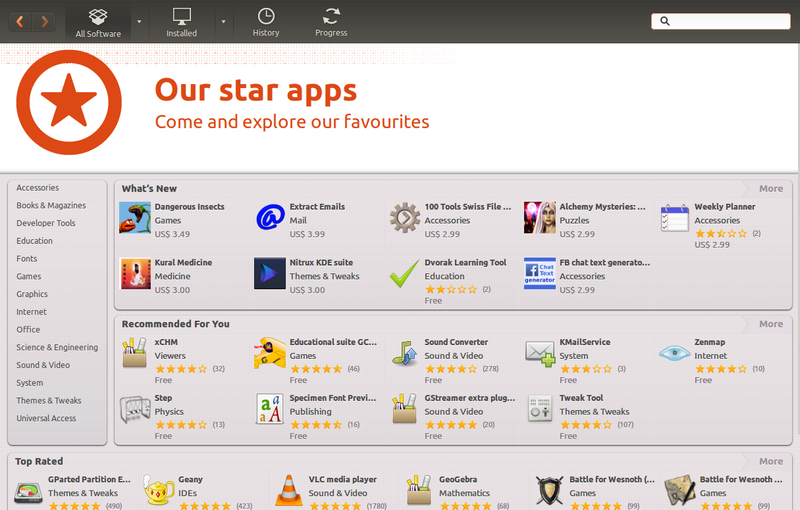
\includegraphics[scale=0.6]{img/ubuntu-software-center.png}}
\caption{Ubuntu Software Center}
\label{fig:ubuntu-software-center}
\end{figure}

There are however certain corner-cases where APT may render
the package management unusable.
For instance package list corruption was faced on several occasions,
in that case APT crashes with segmentation fault
\footnote{http://askubuntu.com/questions/532200/14-04-lts-apt-get-segfault}
and currently the only known solution to the problem
involves deleting package lists and running \emph{apt-get update} again.
Several faulty packaging scripts were stumbled on,
for example it was not possible to remove certain versions of LibreOffice packages
and manual intervention was necessary
\footnote{\url{https://www.linuxquestions.org/questions/showthread.php?s=e0e2f7689f847a56e8cee94a0cafd6bd&p=5216367#post5216367}}.

Debian community has been working hard to provide differential updates for
the packages, but as of February 2015 the efforts have proven fruitless.
Differential updates are applied for package lists
\footnote{\url{https://www.debian-administration.org/article/439/Avoiding_slow_package_updates_with_package_diffs}},
but binary diffs for packages have not implemented yet.
Fedora community has however successfully deployed differential packages
\footnote{http://fedoraproject.org/wiki/Features/Presto},
thus reducing the amount of data needed to be transferred during an package update. For bigger software (eg LibreOffice) the lack of differential updates poses a serious concern, especially for low-bandwidth links.

Release upgrades for example from Ubuntu 12.04 to Ubuntu 14.04
have proven to be especially troublesome due to the fact that system libraries
and files are updated and interrupted release upgrade may leave system
in an unusable state.


\begin{figure}[!htb]
\centering
\scalebox{0.5}{% Graphic for TeX using PGF
% Title: /home/lauri/msc-thesis/dia/traditional-partitioning.dia
% Creator: Dia v0.97.3
% CreationDate: Sun Apr  5 10:02:27 2015
% For: lauri
% \usepackage{tikz}
% The following commands are not supported in PSTricks at present
% We define them conditionally, so when they are implemented,
% this pgf file will use them.
\ifx\du\undefined
  \newlength{\du}
\fi
\setlength{\du}{15\unitlength}
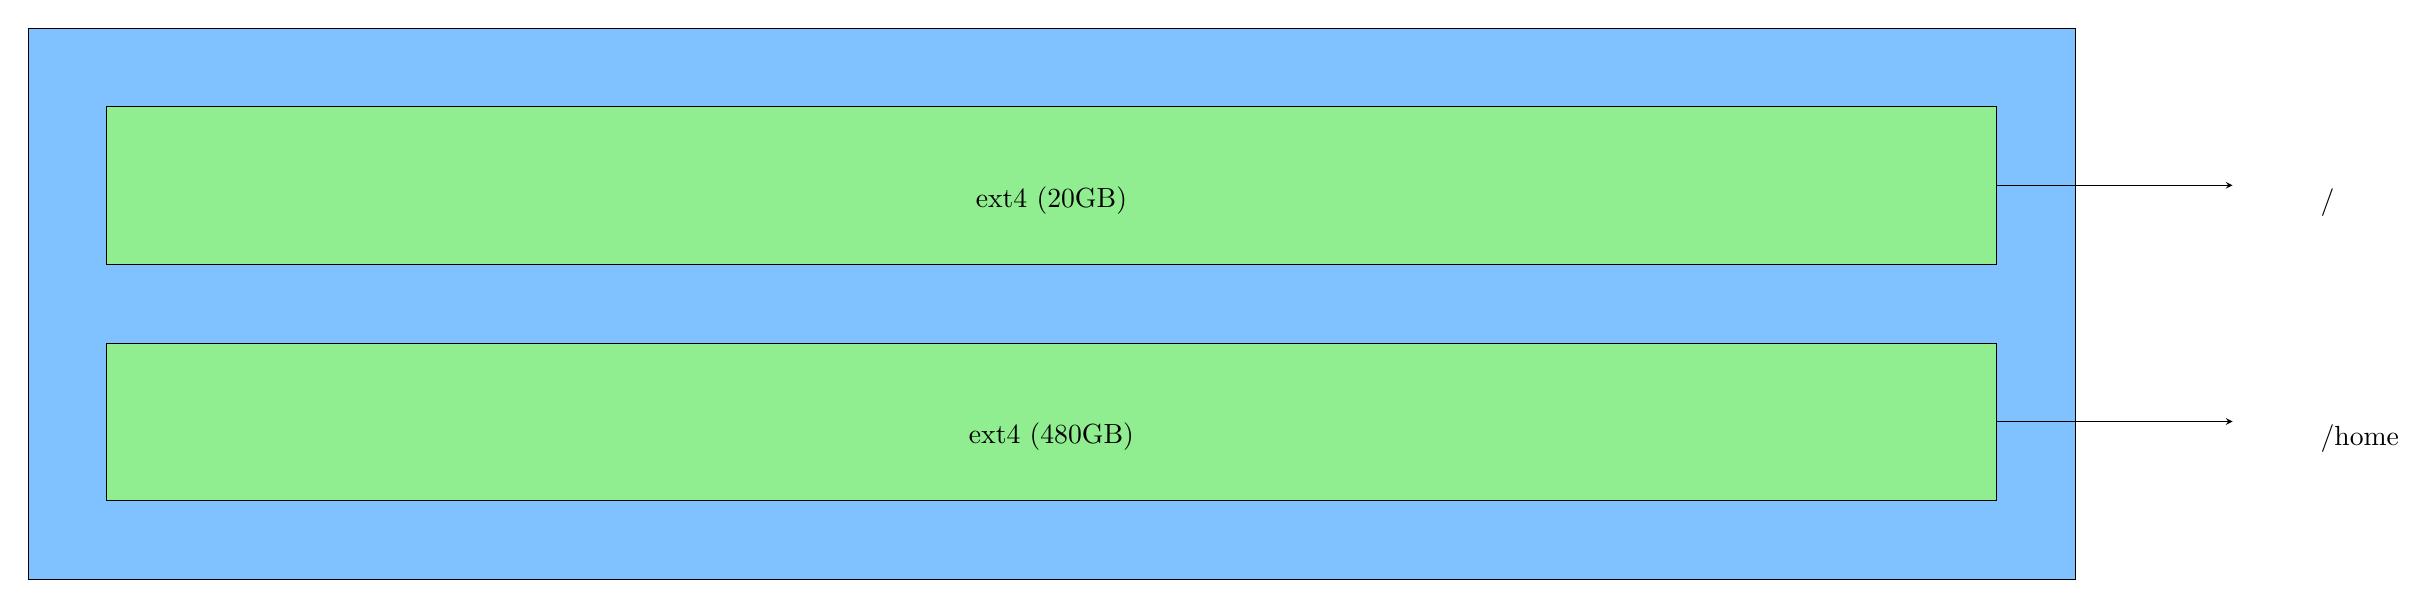
\begin{tikzpicture}
\pgftransformxscale{1.000000}
\pgftransformyscale{-1.000000}
\definecolor{dialinecolor}{rgb}{0.000000, 0.000000, 0.000000}
\pgfsetstrokecolor{dialinecolor}
\definecolor{dialinecolor}{rgb}{1.000000, 1.000000, 1.000000}
\pgfsetfillcolor{dialinecolor}
\pgfsetlinewidth{0.100000\du}
\pgfsetdash{}{0pt}
\pgfsetdash{}{0pt}
\pgfsetmiterjoin
\definecolor{dialinecolor}{rgb}{0.501961, 0.756863, 1.000000}
\pgfsetfillcolor{dialinecolor}
\fill (0.000000\du,0.000000\du)--(0.000000\du,7.000000\du)--(26.000000\du,7.000000\du)--(26.000000\du,0.000000\du)--cycle;
\definecolor{dialinecolor}{rgb}{0.000000, 0.000000, 0.000000}
\pgfsetstrokecolor{dialinecolor}
\draw (0.000000\du,0.000000\du)--(0.000000\du,7.000000\du)--(26.000000\du,7.000000\du)--(26.000000\du,0.000000\du)--cycle;
\definecolor{dialinecolor}{rgb}{0.564706, 0.933333, 0.564706}
\pgfsetfillcolor{dialinecolor}
\fill (1.000000\du,1.000000\du)--(1.000000\du,3.000000\du)--(25.000000\du,3.000000\du)--(25.000000\du,1.000000\du)--cycle;
\pgfsetlinewidth{0.100000\du}
\pgfsetdash{}{0pt}
\pgfsetdash{}{0pt}
\pgfsetmiterjoin
\definecolor{dialinecolor}{rgb}{0.000000, 0.000000, 0.000000}
\pgfsetstrokecolor{dialinecolor}
\draw (1.000000\du,1.000000\du)--(1.000000\du,3.000000\du)--(25.000000\du,3.000000\du)--(25.000000\du,1.000000\du)--cycle;
% setfont left to latex
\definecolor{dialinecolor}{rgb}{0.000000, 0.000000, 0.000000}
\pgfsetstrokecolor{dialinecolor}
\node at (13.000000\du,2.195000\du){ext4 (20GB)};
\pgfsetlinewidth{0.100000\du}
\pgfsetdash{}{0pt}
\pgfsetdash{}{0pt}
\pgfsetbuttcap
{
\definecolor{dialinecolor}{rgb}{0.000000, 0.000000, 0.000000}
\pgfsetfillcolor{dialinecolor}
% was here!!!
\pgfsetarrowsend{stealth}
\definecolor{dialinecolor}{rgb}{0.000000, 0.000000, 0.000000}
\pgfsetstrokecolor{dialinecolor}
\draw (25.000000\du,2.000000\du)--(28.000000\du,2.000000\du);
}
\pgfsetlinewidth{0.100000\du}
\pgfsetdash{}{0pt}
\pgfsetdash{}{0pt}
\pgfsetbuttcap
{
\definecolor{dialinecolor}{rgb}{0.000000, 0.000000, 0.000000}
\pgfsetfillcolor{dialinecolor}
% was here!!!
\pgfsetarrowsend{stealth}
\definecolor{dialinecolor}{rgb}{0.000000, 0.000000, 0.000000}
\pgfsetstrokecolor{dialinecolor}
\draw (25.000000\du,5.000000\du)--(28.000000\du,5.000000\du);
}
% setfont left to latex
\definecolor{dialinecolor}{rgb}{0.000000, 0.000000, 0.000000}
\pgfsetstrokecolor{dialinecolor}
\node[anchor=west] at (29.000000\du,5.221250\du){/home};
% setfont left to latex
\definecolor{dialinecolor}{rgb}{0.000000, 0.000000, 0.000000}
\pgfsetstrokecolor{dialinecolor}
\node[anchor=west] at (29.000000\du,2.221250\du){/};
\definecolor{dialinecolor}{rgb}{0.564706, 0.933333, 0.564706}
\pgfsetfillcolor{dialinecolor}
\fill (1.000000\du,4.000000\du)--(1.000000\du,6.000000\du)--(25.000000\du,6.000000\du)--(25.000000\du,4.000000\du)--cycle;
\pgfsetlinewidth{0.100000\du}
\pgfsetdash{}{0pt}
\pgfsetdash{}{0pt}
\pgfsetmiterjoin
\definecolor{dialinecolor}{rgb}{0.000000, 0.000000, 0.000000}
\pgfsetstrokecolor{dialinecolor}
\draw (1.000000\du,4.000000\du)--(1.000000\du,6.000000\du)--(25.000000\du,6.000000\du)--(25.000000\du,4.000000\du)--cycle;
% setfont left to latex
\definecolor{dialinecolor}{rgb}{0.000000, 0.000000, 0.000000}
\pgfsetstrokecolor{dialinecolor}
\node at (13.000000\du,5.195000\du){ext4 (480GB)};
\end{tikzpicture}
}
\caption{Partitioning with separate /home}
\label{fig:traditional-partitioning}
\end{figure}

Even so separate filesystem for home directories has
proven to be effective method against wiping the whole disk
during reinstall of Ubuntu.

Puppet, SaltStack, Chef, Ansible and other traditional configuration
management fit best the scenario where each node has slightly different
configuration and it makes sense to keep them separate. However
provisioning very similar nodes with for instance Foreman has obvious
overhead - each node has to fetch updated packages independently from
the same APT repositories, same has to be done for application software.

For classroom deployment cloning has been used in the past:
Windows, Ubuntu or both are installed on a physical template machine.
Template machine is thoroughly tested.
Tools such as Clonezilla or Symantec Ghost are used to transfer the
harddisk image to the other machines.
As the whole procedure is a complex undertaking
it is usually performed once a year in summer especially for educational

The workflow for the prototype is described in Figure
~\ref{fig:butterknife-workflow}





\section{Prototype}


The prototype draws inspiration from embedded computers
where certain guarantees have to be provided.



\begin{figure}[!htb]
\centering
\scalebox{0.5}{% Graphic for TeX using PGF
% Title: /home/lauri/Projektid/blog/pages/cloning/dia/workflow-en.dia
% Creator: Dia v0.97.2
% CreationDate: Thu Feb 26 18:06:28 2015
% For: lauri
% \usepackage{tikz}
% The following commands are not supported in PSTricks at present
% We define them conditionally, so when they are implemented,
% this pgf file will use them.
\ifx\du\undefined
  \newlength{\du}
\fi
\setlength{\du}{15\unitlength}
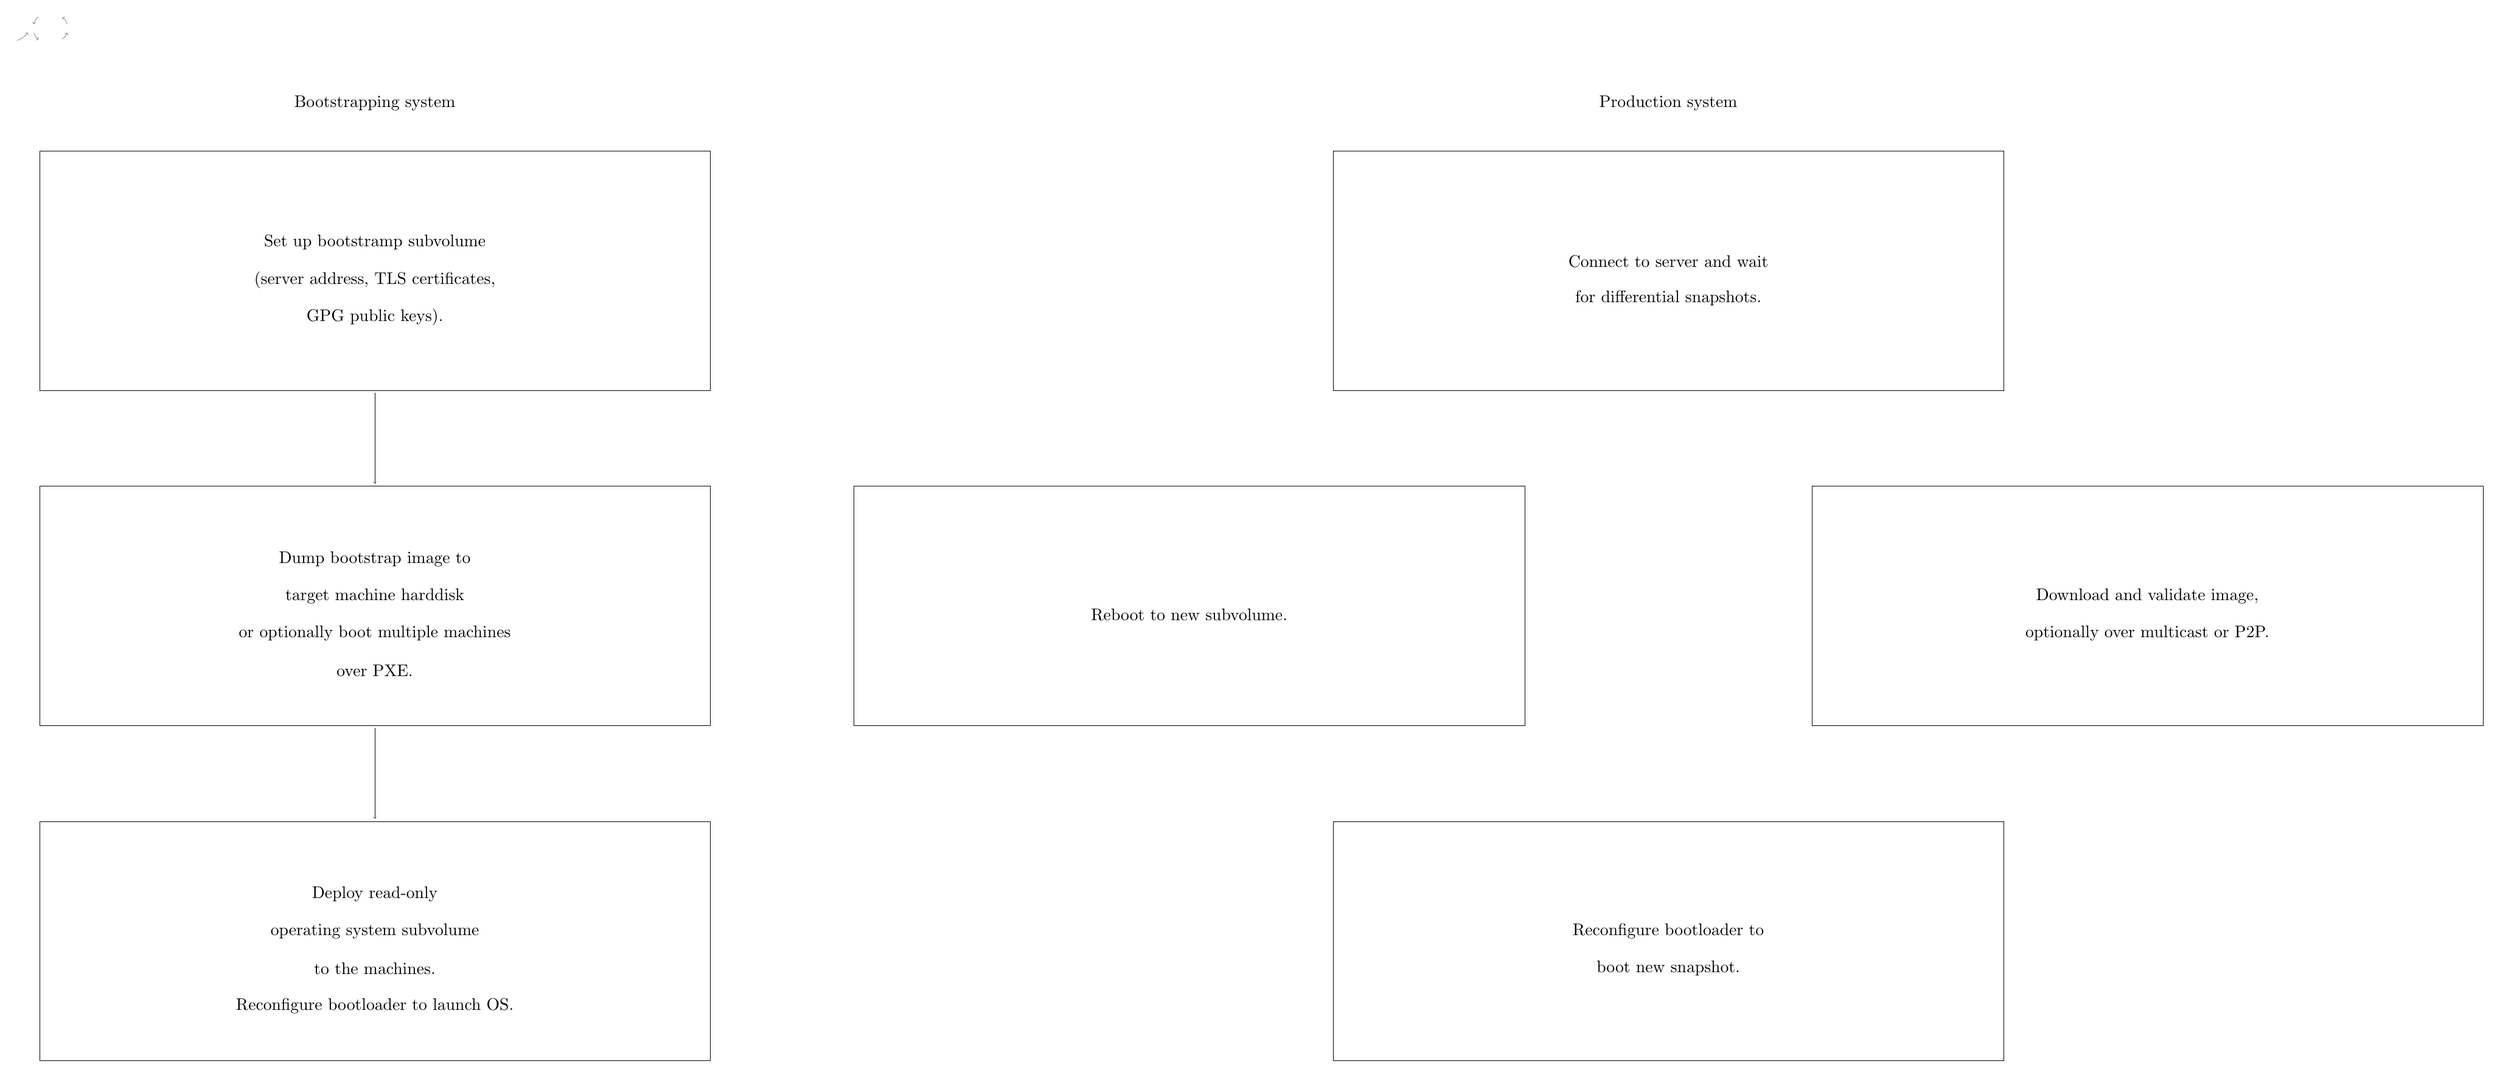
\begin{tikzpicture}
\pgftransformxscale{1.000000}
\pgftransformyscale{-1.000000}
\definecolor{dialinecolor}{rgb}{0.000000, 0.000000, 0.000000}
\pgfsetstrokecolor{dialinecolor}
\definecolor{dialinecolor}{rgb}{1.000000, 1.000000, 1.000000}
\pgfsetfillcolor{dialinecolor}
% setfont left to latex
\definecolor{dialinecolor}{rgb}{0.000000, 0.000000, 0.000000}
\pgfsetstrokecolor{dialinecolor}
\node at (8.000000\du,2.000000\du){Bootstrapping system};
\definecolor{dialinecolor}{rgb}{1.000000, 1.000000, 1.000000}
\pgfsetfillcolor{dialinecolor}
\fill (1.000000\du,3.000000\du)--(1.000000\du,8.000000\du)--(15.000000\du,8.000000\du)--(15.000000\du,3.000000\du)--cycle;
\pgfsetlinewidth{0.100000\du}
\pgfsetdash{}{0pt}
\pgfsetdash{}{0pt}
\pgfsetmiterjoin
\definecolor{dialinecolor}{rgb}{0.000000, 0.000000, 0.000000}
\pgfsetstrokecolor{dialinecolor}
\draw (1.000000\du,3.000000\du)--(1.000000\du,8.000000\du)--(15.000000\du,8.000000\du)--(15.000000\du,3.000000\du)--cycle;
% setfont left to latex
\definecolor{dialinecolor}{rgb}{0.000000, 0.000000, 0.000000}
\pgfsetstrokecolor{dialinecolor}
\node at (8.000000\du,4.913333\du){Set up bootstramp subvolume};
% setfont left to latex
\definecolor{dialinecolor}{rgb}{0.000000, 0.000000, 0.000000}
\pgfsetstrokecolor{dialinecolor}
\node at (8.000000\du,5.689444\du){(server address, TLS certificates,};
% setfont left to latex
\definecolor{dialinecolor}{rgb}{0.000000, 0.000000, 0.000000}
\pgfsetstrokecolor{dialinecolor}
\node at (8.000000\du,6.465556\du){GPG public keys).};
\definecolor{dialinecolor}{rgb}{1.000000, 1.000000, 1.000000}
\pgfsetfillcolor{dialinecolor}
\fill (1.000000\du,10.000000\du)--(1.000000\du,15.000000\du)--(15.000000\du,15.000000\du)--(15.000000\du,10.000000\du)--cycle;
\pgfsetlinewidth{0.100000\du}
\pgfsetdash{}{0pt}
\pgfsetdash{}{0pt}
\pgfsetmiterjoin
\definecolor{dialinecolor}{rgb}{0.000000, 0.000000, 0.000000}
\pgfsetstrokecolor{dialinecolor}
\draw (1.000000\du,10.000000\du)--(1.000000\du,15.000000\du)--(15.000000\du,15.000000\du)--(15.000000\du,10.000000\du)--cycle;
% setfont left to latex
\definecolor{dialinecolor}{rgb}{0.000000, 0.000000, 0.000000}
\pgfsetstrokecolor{dialinecolor}
\node at (8.000000\du,11.525278\du){Dump bootstrap image to};
% setfont left to latex
\definecolor{dialinecolor}{rgb}{0.000000, 0.000000, 0.000000}
\pgfsetstrokecolor{dialinecolor}
\node at (8.000000\du,12.301389\du){target machine harddisk};
% setfont left to latex
\definecolor{dialinecolor}{rgb}{0.000000, 0.000000, 0.000000}
\pgfsetstrokecolor{dialinecolor}
\node at (8.000000\du,13.077500\du){or optionally boot multiple machines};
% setfont left to latex
\definecolor{dialinecolor}{rgb}{0.000000, 0.000000, 0.000000}
\pgfsetstrokecolor{dialinecolor}
\node at (8.000000\du,13.853611\du){over PXE.};
\pgfsetlinewidth{0.100000\du}
\pgfsetdash{}{0pt}
\pgfsetdash{}{0pt}
\pgfsetbuttcap
{
\definecolor{dialinecolor}{rgb}{0.000000, 0.000000, 0.000000}
\pgfsetfillcolor{dialinecolor}
% was here!!!
\pgfsetarrowsend{to}
\definecolor{dialinecolor}{rgb}{0.000000, 0.000000, 0.000000}
\pgfsetstrokecolor{dialinecolor}
\draw (8.000000\du,8.050232\du)--(8.000000\du,9.949768\du);
}
\definecolor{dialinecolor}{rgb}{1.000000, 1.000000, 1.000000}
\pgfsetfillcolor{dialinecolor}
\fill (1.000000\du,17.000000\du)--(1.000000\du,22.000000\du)--(15.000000\du,22.000000\du)--(15.000000\du,17.000000\du)--cycle;
\pgfsetlinewidth{0.100000\du}
\pgfsetdash{}{0pt}
\pgfsetdash{}{0pt}
\pgfsetmiterjoin
\definecolor{dialinecolor}{rgb}{0.000000, 0.000000, 0.000000}
\pgfsetstrokecolor{dialinecolor}
\draw (1.000000\du,17.000000\du)--(1.000000\du,22.000000\du)--(15.000000\du,22.000000\du)--(15.000000\du,17.000000\du)--cycle;
% setfont left to latex
\definecolor{dialinecolor}{rgb}{0.000000, 0.000000, 0.000000}
\pgfsetstrokecolor{dialinecolor}
\node at (8.000000\du,18.525278\du){Deploy read-only};
% setfont left to latex
\definecolor{dialinecolor}{rgb}{0.000000, 0.000000, 0.000000}
\pgfsetstrokecolor{dialinecolor}
\node at (8.000000\du,19.301389\du){operating system subvolume};
% setfont left to latex
\definecolor{dialinecolor}{rgb}{0.000000, 0.000000, 0.000000}
\pgfsetstrokecolor{dialinecolor}
\node at (8.000000\du,20.077500\du){to the machines.};
% setfont left to latex
\definecolor{dialinecolor}{rgb}{0.000000, 0.000000, 0.000000}
\pgfsetstrokecolor{dialinecolor}
\node at (8.000000\du,20.853611\du){Reconfigure bootloader to launch OS.};
\pgfsetlinewidth{0.100000\du}
\pgfsetdash{}{0pt}
\pgfsetdash{}{0pt}
\pgfsetbuttcap
{
\definecolor{dialinecolor}{rgb}{0.000000, 0.000000, 0.000000}
\pgfsetfillcolor{dialinecolor}
% was here!!!
\pgfsetarrowsend{to}
\definecolor{dialinecolor}{rgb}{0.000000, 0.000000, 0.000000}
\pgfsetstrokecolor{dialinecolor}
\draw (8.000000\du,15.050232\du)--(8.000000\du,16.949768\du);
}
\definecolor{dialinecolor}{rgb}{1.000000, 1.000000, 1.000000}
\pgfsetfillcolor{dialinecolor}
\fill (28.000000\du,3.000000\du)--(28.000000\du,8.000000\du)--(42.000000\du,8.000000\du)--(42.000000\du,3.000000\du)--cycle;
\pgfsetlinewidth{0.100000\du}
\pgfsetdash{}{0pt}
\pgfsetdash{}{0pt}
\pgfsetmiterjoin
\definecolor{dialinecolor}{rgb}{0.000000, 0.000000, 0.000000}
\pgfsetstrokecolor{dialinecolor}
\draw (28.000000\du,3.000000\du)--(28.000000\du,8.000000\du)--(42.000000\du,8.000000\du)--(42.000000\du,3.000000\du)--cycle;
% setfont left to latex
\definecolor{dialinecolor}{rgb}{0.000000, 0.000000, 0.000000}
\pgfsetstrokecolor{dialinecolor}
\node at (35.000000\du,5.301389\du){Connect to server and wait};
% setfont left to latex
\definecolor{dialinecolor}{rgb}{0.000000, 0.000000, 0.000000}
\pgfsetstrokecolor{dialinecolor}
\node at (35.000000\du,6.077500\du){for differential snapshots.};
\definecolor{dialinecolor}{rgb}{1.000000, 1.000000, 1.000000}
\pgfsetfillcolor{dialinecolor}
\fill (18.000000\du,10.000000\du)--(18.000000\du,15.000000\du)--(32.000000\du,15.000000\du)--(32.000000\du,10.000000\du)--cycle;
\pgfsetlinewidth{0.100000\du}
\pgfsetdash{}{0pt}
\pgfsetdash{}{0pt}
\pgfsetmiterjoin
\definecolor{dialinecolor}{rgb}{0.000000, 0.000000, 0.000000}
\pgfsetstrokecolor{dialinecolor}
\draw (18.000000\du,10.000000\du)--(18.000000\du,15.000000\du)--(32.000000\du,15.000000\du)--(32.000000\du,10.000000\du)--cycle;
% setfont left to latex
\definecolor{dialinecolor}{rgb}{0.000000, 0.000000, 0.000000}
\pgfsetstrokecolor{dialinecolor}
\node at (25.000000\du,12.689444\du){Reboot to new subvolume.};
\pgfsetlinewidth{0.100000\du}
\pgfsetdash{}{0pt}
\pgfsetdash{}{0pt}
\pgfsetbuttcap
{
\definecolor{dialinecolor}{rgb}{0.000000, 0.000000, 0.000000}
\pgfsetfillcolor{dialinecolor}
% was here!!!
\pgfsetarrowsend{to}
\definecolor{dialinecolor}{rgb}{0.000000, 0.000000, 0.000000}
\pgfsetstrokecolor{dialinecolor}
\pgfpathmoveto{\pgfpoint{15.049490\du}{19.640275\du}}
\pgfpatharc{74}{35}{11.858541\du and 11.858541\du}
\pgfusepath{stroke}
}
\definecolor{dialinecolor}{rgb}{1.000000, 1.000000, 1.000000}
\pgfsetfillcolor{dialinecolor}
\fill (28.000000\du,17.000000\du)--(28.000000\du,22.000000\du)--(42.000000\du,22.000000\du)--(42.000000\du,17.000000\du)--cycle;
\pgfsetlinewidth{0.100000\du}
\pgfsetdash{}{0pt}
\pgfsetdash{}{0pt}
\pgfsetmiterjoin
\definecolor{dialinecolor}{rgb}{0.000000, 0.000000, 0.000000}
\pgfsetstrokecolor{dialinecolor}
\draw (28.000000\du,17.000000\du)--(28.000000\du,22.000000\du)--(42.000000\du,22.000000\du)--(42.000000\du,17.000000\du)--cycle;
% setfont left to latex
\definecolor{dialinecolor}{rgb}{0.000000, 0.000000, 0.000000}
\pgfsetstrokecolor{dialinecolor}
\node at (35.000000\du,19.301389\du){Reconfigure bootloader to};
% setfont left to latex
\definecolor{dialinecolor}{rgb}{0.000000, 0.000000, 0.000000}
\pgfsetstrokecolor{dialinecolor}
\node at (35.000000\du,20.077500\du){boot new snapshot.};
\definecolor{dialinecolor}{rgb}{1.000000, 1.000000, 1.000000}
\pgfsetfillcolor{dialinecolor}
\fill (38.000000\du,10.000000\du)--(38.000000\du,15.000000\du)--(52.000000\du,15.000000\du)--(52.000000\du,10.000000\du)--cycle;
\pgfsetlinewidth{0.100000\du}
\pgfsetdash{}{0pt}
\pgfsetdash{}{0pt}
\pgfsetmiterjoin
\definecolor{dialinecolor}{rgb}{0.000000, 0.000000, 0.000000}
\pgfsetstrokecolor{dialinecolor}
\draw (38.000000\du,10.000000\du)--(38.000000\du,15.000000\du)--(52.000000\du,15.000000\du)--(52.000000\du,10.000000\du)--cycle;
% setfont left to latex
\definecolor{dialinecolor}{rgb}{0.000000, 0.000000, 0.000000}
\pgfsetstrokecolor{dialinecolor}
\node at (45.000000\du,12.301389\du){Download and validate image,};
% setfont left to latex
\definecolor{dialinecolor}{rgb}{0.000000, 0.000000, 0.000000}
\pgfsetstrokecolor{dialinecolor}
\node at (45.000000\du,13.077500\du){optionally over multicast or P2P.};
\pgfsetlinewidth{0.100000\du}
\pgfsetdash{}{0pt}
\pgfsetdash{}{0pt}
\pgfsetbuttcap
{
\definecolor{dialinecolor}{rgb}{0.000000, 0.000000, 0.000000}
\pgfsetfillcolor{dialinecolor}
% was here!!!
\pgfsetarrowsend{to}
\definecolor{dialinecolor}{rgb}{0.000000, 0.000000, 0.000000}
\pgfsetstrokecolor{dialinecolor}
\pgfpathmoveto{\pgfpoint{27.950110\du}{5.675501\du}}
\pgfpatharc{237}{192}{6.723537\du and 6.723537\du}
\pgfusepath{stroke}
}
\pgfsetlinewidth{0.100000\du}
\pgfsetdash{}{0pt}
\pgfsetdash{}{0pt}
\pgfsetbuttcap
{
\definecolor{dialinecolor}{rgb}{0.000000, 0.000000, 0.000000}
\pgfsetfillcolor{dialinecolor}
% was here!!!
\pgfsetarrowsend{to}
\definecolor{dialinecolor}{rgb}{0.000000, 0.000000, 0.000000}
\pgfsetstrokecolor{dialinecolor}
\pgfpathmoveto{\pgfpoint{44.870667\du}{9.950218\du}}
\pgfpatharc{347}{305}{6.860399\du and 6.860399\du}
\pgfusepath{stroke}
}
\pgfsetlinewidth{0.100000\du}
\pgfsetdash{}{0pt}
\pgfsetdash{}{0pt}
\pgfsetbuttcap
{
\definecolor{dialinecolor}{rgb}{0.000000, 0.000000, 0.000000}
\pgfsetfillcolor{dialinecolor}
% was here!!!
\pgfsetarrowsend{to}
\definecolor{dialinecolor}{rgb}{0.000000, 0.000000, 0.000000}
\pgfsetstrokecolor{dialinecolor}
\pgfpathmoveto{\pgfpoint{42.049045\du}{18.901522\du}}
\pgfpatharc{55}{16}{7.019442\du and 7.019442\du}
\pgfusepath{stroke}
}
\pgfsetlinewidth{0.100000\du}
\pgfsetdash{}{0pt}
\pgfsetdash{}{0pt}
\pgfsetbuttcap
{
\definecolor{dialinecolor}{rgb}{0.000000, 0.000000, 0.000000}
\pgfsetfillcolor{dialinecolor}
% was here!!!
\pgfsetarrowsend{to}
\definecolor{dialinecolor}{rgb}{0.000000, 0.000000, 0.000000}
\pgfsetstrokecolor{dialinecolor}
\pgfpathmoveto{\pgfpoint{25.129248\du}{15.049431\du}}
\pgfpatharc{167}{125}{6.860399\du and 6.860399\du}
\pgfusepath{stroke}
}
% setfont left to latex
\definecolor{dialinecolor}{rgb}{0.000000, 0.000000, 0.000000}
\pgfsetstrokecolor{dialinecolor}
\node at (35.000000\du,2.000000\du){Production system};
\end{tikzpicture}
}
\caption{Workflow for btrfs snapshot based software deployment}
\label{fig:butterknife-workflow}
\end{figure}





\begin{figure}[!htb]
\centering
\scalebox{0.5}{% Graphic for TeX using PGF
% Title: /home/lauri/Projektid/msc-thesis/dia/butterknife-usecase-http.dia
% Creator: Dia v0.97.2
% CreationDate: Sun Mar 15 12:52:30 2015
% For: lauri
% \usepackage{tikz}
% The following commands are not supported in PSTricks at present
% We define them conditionally, so when they are implemented,
% this pgf file will use them.
\ifx\du\undefined
  \newlength{\du}
\fi
\setlength{\du}{15\unitlength}
\begin{tikzpicture}
\pgftransformxscale{1.000000}
\pgftransformyscale{-1.000000}
\definecolor{dialinecolor}{rgb}{0.000000, 0.000000, 0.000000}
\pgfsetstrokecolor{dialinecolor}
\definecolor{dialinecolor}{rgb}{1.000000, 1.000000, 1.000000}
\pgfsetfillcolor{dialinecolor}
\pgfsetlinewidth{0.100000\du}
\pgfsetdash{}{0pt}
\pgfsetdash{}{0pt}
\pgfsetbuttcap
\pgfsetmiterjoin
\pgfsetlinewidth{0.001000\du}
\pgfsetbuttcap
\pgfsetmiterjoin
\pgfsetdash{}{0pt}
\definecolor{dialinecolor}{rgb}{0.647059, 0.647059, 0.521569}
\pgfsetfillcolor{dialinecolor}
\pgfpathmoveto{\pgfpoint{16.000000\du}{5.123976\du}}
\pgfpathlineto{\pgfpoint{15.997269\du}{5.089022\du}}
\pgfpathlineto{\pgfpoint{15.989623\du}{5.054615\du}}
\pgfpathlineto{\pgfpoint{15.976516\du}{5.020208\du}}
\pgfpathlineto{\pgfpoint{15.958493\du}{4.986346\du}}
\pgfpathlineto{\pgfpoint{15.936100\du}{4.952485\du}}
\pgfpathlineto{\pgfpoint{15.908247\du}{4.919170\du}}
\pgfpathlineto{\pgfpoint{15.875478\du}{4.886401\du}}
\pgfpathlineto{\pgfpoint{15.837794\du}{4.854178\du}}
\pgfpathlineto{\pgfpoint{15.795194\du}{4.822501\du}}
\pgfpathlineto{\pgfpoint{15.748225\du}{4.792463\du}}
\pgfpathlineto{\pgfpoint{15.696887\du}{4.762425\du}}
\pgfpathlineto{\pgfpoint{15.641726\du}{4.732933\du}}
\pgfpathlineto{\pgfpoint{15.581103\du}{4.705079\du}}
\pgfpathlineto{\pgfpoint{15.517204\du}{4.678318\du}}
\pgfpathlineto{\pgfpoint{15.449481\du}{4.652649\du}}
\pgfpathlineto{\pgfpoint{15.377389\du}{4.628072\du}}
\pgfpathlineto{\pgfpoint{15.302567\du}{4.605134\du}}
\pgfpathlineto{\pgfpoint{15.223921\du}{4.583288\du}}
\pgfpathlineto{\pgfpoint{15.142545\du}{4.563080\du}}
\pgfpathlineto{\pgfpoint{15.057346\du}{4.543965\du}}
\pgfpathlineto{\pgfpoint{14.970508\du}{4.525942\du}}
\pgfpathlineto{\pgfpoint{14.880393\du}{4.510104\du}}
\pgfpathlineto{\pgfpoint{14.788094\du}{4.494812\du}}
\pgfpathlineto{\pgfpoint{14.694702\du}{4.482250\du}}
\pgfpathlineto{\pgfpoint{14.598580\du}{4.471327\du}}
\pgfpathlineto{\pgfpoint{14.500819\du}{4.462043\du}}
\pgfpathlineto{\pgfpoint{14.402512\du}{4.453850\du}}
\pgfpathlineto{\pgfpoint{14.302567\du}{4.448389\du}}
\pgfpathlineto{\pgfpoint{14.202075\du}{4.443474\du}}
\pgfpathlineto{\pgfpoint{14.101038\du}{4.440197\du}}
\pgfpathlineto{\pgfpoint{14.000000\du}{4.440197\du}}
\pgfpathlineto{\pgfpoint{14.000000\du}{4.440197\du}}
\pgfpathlineto{\pgfpoint{13.898416\du}{4.440197\du}}
\pgfpathlineto{\pgfpoint{13.797378\du}{4.443474\du}}
\pgfpathlineto{\pgfpoint{13.696887\du}{4.448389\du}}
\pgfpathlineto{\pgfpoint{13.596942\du}{4.453850\du}}
\pgfpathlineto{\pgfpoint{13.498635\du}{4.462043\du}}
\pgfpathlineto{\pgfpoint{13.400874\du}{4.471327\du}}
\pgfpathlineto{\pgfpoint{13.305298\du}{4.482250\du}}
\pgfpathlineto{\pgfpoint{13.211360\du}{4.494812\du}}
\pgfpathlineto{\pgfpoint{13.119061\du}{4.510104\du}}
\pgfpathlineto{\pgfpoint{13.028946\du}{4.525942\du}}
\pgfpathlineto{\pgfpoint{12.942108\du}{4.543965\du}}
\pgfpathlineto{\pgfpoint{12.857455\du}{4.563080\du}}
\pgfpathlineto{\pgfpoint{12.776079\du}{4.583288\du}}
\pgfpathlineto{\pgfpoint{12.697433\du}{4.605134\du}}
\pgfpathlineto{\pgfpoint{12.622064\du}{4.628072\du}}
\pgfpathlineto{\pgfpoint{12.549973\du}{4.652649\du}}
\pgfpathlineto{\pgfpoint{12.482796\du}{4.678318\du}}
\pgfpathlineto{\pgfpoint{12.418351\du}{4.705079\du}}
\pgfpathlineto{\pgfpoint{12.358274\du}{4.732933\du}}
\pgfpathlineto{\pgfpoint{12.302567\du}{4.762425\du}}
\pgfpathlineto{\pgfpoint{12.251229\du}{4.792463\du}}
\pgfpathlineto{\pgfpoint{12.204260\du}{4.822501\du}}
\pgfpathlineto{\pgfpoint{12.161660\du}{4.854178\du}}
\pgfpathlineto{\pgfpoint{12.123976\du}{4.886401\du}}
\pgfpathlineto{\pgfpoint{12.091207\du}{4.919170\du}}
\pgfpathlineto{\pgfpoint{12.063353\du}{4.952485\du}}
\pgfpathlineto{\pgfpoint{12.040961\du}{4.986346\du}}
\pgfpathlineto{\pgfpoint{12.022938\du}{5.020208\du}}
\pgfpathlineto{\pgfpoint{12.009831\du}{5.054615\du}}
\pgfpathlineto{\pgfpoint{12.002731\du}{5.089022\du}}
\pgfpathlineto{\pgfpoint{12.000000\du}{5.123976\du}}
\pgfpathlineto{\pgfpoint{12.000000\du}{5.123976\du}}
\pgfpathlineto{\pgfpoint{12.002731\du}{5.158930\du}}
\pgfpathlineto{\pgfpoint{12.009831\du}{5.192791\du}}
\pgfpathlineto{\pgfpoint{12.022938\du}{5.227744\du}}
\pgfpathlineto{\pgfpoint{12.040961\du}{5.261606\du}}
\pgfpathlineto{\pgfpoint{12.063353\du}{5.295467\du}}
\pgfpathlineto{\pgfpoint{12.091207\du}{5.328782\du}}
\pgfpathlineto{\pgfpoint{12.123976\du}{5.361551\du}}
\pgfpathlineto{\pgfpoint{12.161660\du}{5.393774\du}}
\pgfpathlineto{\pgfpoint{12.204260\du}{5.424904\du}}
\pgfpathlineto{\pgfpoint{12.251229\du}{5.455489\du}}
\pgfpathlineto{\pgfpoint{12.302567\du}{5.485527\du}}
\pgfpathlineto{\pgfpoint{12.358274\du}{5.515019\du}}
\pgfpathlineto{\pgfpoint{12.418351\du}{5.542873\du}}
\pgfpathlineto{\pgfpoint{12.482796\du}{5.569634\du}}
\pgfpathlineto{\pgfpoint{12.549973\du}{5.595303\du}}
\pgfpathlineto{\pgfpoint{12.622064\du}{5.619880\du}}
\pgfpathlineto{\pgfpoint{12.697433\du}{5.642818\du}}
\pgfpathlineto{\pgfpoint{12.776079\du}{5.664664\du}}
\pgfpathlineto{\pgfpoint{12.857455\du}{5.684872\du}}
\pgfpathlineto{\pgfpoint{12.942108\du}{5.703987\du}}
\pgfpathlineto{\pgfpoint{13.028946\du}{5.722010\du}}
\pgfpathlineto{\pgfpoint{13.119061\du}{5.737848\du}}
\pgfpathlineto{\pgfpoint{13.211360\du}{5.752594\du}}
\pgfpathlineto{\pgfpoint{13.305298\du}{5.765702\du}}
\pgfpathlineto{\pgfpoint{13.400874\du}{5.776625\du}}
\pgfpathlineto{\pgfpoint{13.498635\du}{5.785909\du}}
\pgfpathlineto{\pgfpoint{13.596942\du}{5.793555\du}}
\pgfpathlineto{\pgfpoint{13.696887\du}{5.799563\du}}
\pgfpathlineto{\pgfpoint{13.797378\du}{5.803932\du}}
\pgfpathlineto{\pgfpoint{13.898416\du}{5.807209\du}}
\pgfpathlineto{\pgfpoint{14.000000\du}{5.807755\du}}
\pgfpathlineto{\pgfpoint{14.000000\du}{5.807755\du}}
\pgfpathlineto{\pgfpoint{14.101038\du}{5.807209\du}}
\pgfpathlineto{\pgfpoint{14.202075\du}{5.803932\du}}
\pgfpathlineto{\pgfpoint{14.302567\du}{5.799563\du}}
\pgfpathlineto{\pgfpoint{14.402512\du}{5.793555\du}}
\pgfpathlineto{\pgfpoint{14.500819\du}{5.785909\du}}
\pgfpathlineto{\pgfpoint{14.598580\du}{5.776625\du}}
\pgfpathlineto{\pgfpoint{14.694702\du}{5.765702\du}}
\pgfpathlineto{\pgfpoint{14.788094\du}{5.752594\du}}
\pgfpathlineto{\pgfpoint{14.880393\du}{5.737848\du}}
\pgfpathlineto{\pgfpoint{14.970508\du}{5.722010\du}}
\pgfpathlineto{\pgfpoint{15.057346\du}{5.703987\du}}
\pgfpathlineto{\pgfpoint{15.142545\du}{5.684872\du}}
\pgfpathlineto{\pgfpoint{15.223921\du}{5.664664\du}}
\pgfpathlineto{\pgfpoint{15.302567\du}{5.642818\du}}
\pgfpathlineto{\pgfpoint{15.377389\du}{5.619880\du}}
\pgfpathlineto{\pgfpoint{15.449481\du}{5.595303\du}}
\pgfpathlineto{\pgfpoint{15.517204\du}{5.569634\du}}
\pgfpathlineto{\pgfpoint{15.581103\du}{5.542873\du}}
\pgfpathlineto{\pgfpoint{15.641726\du}{5.515019\du}}
\pgfpathlineto{\pgfpoint{15.696887\du}{5.485527\du}}
\pgfpathlineto{\pgfpoint{15.748225\du}{5.455489\du}}
\pgfpathlineto{\pgfpoint{15.795194\du}{5.424904\du}}
\pgfpathlineto{\pgfpoint{15.837794\du}{5.393774\du}}
\pgfpathlineto{\pgfpoint{15.875478\du}{5.361551\du}}
\pgfpathlineto{\pgfpoint{15.908247\du}{5.328782\du}}
\pgfpathlineto{\pgfpoint{15.936100\du}{5.295467\du}}
\pgfpathlineto{\pgfpoint{15.958493\du}{5.261606\du}}
\pgfpathlineto{\pgfpoint{15.976516\du}{5.227744\du}}
\pgfpathlineto{\pgfpoint{15.989623\du}{5.192791\du}}
\pgfpathlineto{\pgfpoint{15.997269\du}{5.158930\du}}
\pgfpathlineto{\pgfpoint{16.000000\du}{5.123976\du}}
\pgfusepath{fill}
\pgfsetbuttcap
\pgfsetmiterjoin
\pgfsetdash{}{0pt}
\definecolor{dialinecolor}{rgb}{0.286275, 0.286275, 0.211765}
\pgfsetstrokecolor{dialinecolor}
\pgfpathmoveto{\pgfpoint{15.976516\du}{5.113053\du}}
\pgfpathlineto{\pgfpoint{15.973785\du}{5.078099\du}}
\pgfpathlineto{\pgfpoint{15.966685\du}{5.044784\du}}
\pgfpathlineto{\pgfpoint{15.954123\du}{5.010923\du}}
\pgfpathlineto{\pgfpoint{15.936647\du}{4.977608\du}}
\pgfpathlineto{\pgfpoint{15.913162\du}{4.943747\du}}
\pgfpathlineto{\pgfpoint{15.884762\du}{4.911524\du}}
\pgfpathlineto{\pgfpoint{15.853632\du}{4.878755\du}}
\pgfpathlineto{\pgfpoint{15.815401\du}{4.848170\du}}
\pgfpathlineto{\pgfpoint{15.773348\du}{4.817040\du}}
\pgfpathlineto{\pgfpoint{15.726925\du}{4.786455\du}}
\pgfpathlineto{\pgfpoint{15.675587\du}{4.757510\du}}
\pgfpathlineto{\pgfpoint{15.620426\du}{4.728564\du}}
\pgfpathlineto{\pgfpoint{15.560896\du}{4.701256\du}}
\pgfpathlineto{\pgfpoint{15.498088\du}{4.673949\du}}
\pgfpathlineto{\pgfpoint{15.429274\du}{4.649372\du}}
\pgfpathlineto{\pgfpoint{15.357728\du}{4.625341\du}}
\pgfpathlineto{\pgfpoint{15.282906\du}{4.602403\du}}
\pgfpathlineto{\pgfpoint{15.205352\du}{4.581103\du}}
\pgfpathlineto{\pgfpoint{15.124522\du}{4.561442\du}}
\pgfpathlineto{\pgfpoint{15.040415\du}{4.542327\du}}
\pgfpathlineto{\pgfpoint{14.953031\du}{4.525396\du}}
\pgfpathlineto{\pgfpoint{14.864009\du}{4.509558\du}}
\pgfpathlineto{\pgfpoint{14.772256\du}{4.494812\du}}
\pgfpathlineto{\pgfpoint{14.679410\du}{4.482250\du}}
\pgfpathlineto{\pgfpoint{14.584380\du}{4.471327\du}}
\pgfpathlineto{\pgfpoint{14.486619\du}{4.462589\du}}
\pgfpathlineto{\pgfpoint{14.388859\du}{4.453850\du}}
\pgfpathlineto{\pgfpoint{14.289459\du}{4.448935\du}}
\pgfpathlineto{\pgfpoint{14.190060\du}{4.444566\du}}
\pgfpathlineto{\pgfpoint{14.088476\du}{4.441835\du}}
\pgfpathlineto{\pgfpoint{13.987985\du}{4.440197\du}}
\pgfpathlineto{\pgfpoint{13.987985\du}{4.440197\du}}
\pgfpathlineto{\pgfpoint{13.887493\du}{4.441835\du}}
\pgfpathlineto{\pgfpoint{13.787002\du}{4.444566\du}}
\pgfpathlineto{\pgfpoint{13.686510\du}{4.448935\du}}
\pgfpathlineto{\pgfpoint{13.588203\du}{4.453850\du}}
\pgfpathlineto{\pgfpoint{13.489896\du}{4.462589\du}}
\pgfpathlineto{\pgfpoint{13.392682\du}{4.471327\du}}
\pgfpathlineto{\pgfpoint{13.297105\du}{4.482250\du}}
\pgfpathlineto{\pgfpoint{13.203714\du}{4.494812\du}}
\pgfpathlineto{\pgfpoint{13.112507\du}{4.509558\du}}
\pgfpathlineto{\pgfpoint{13.023484\du}{4.525396\du}}
\pgfpathlineto{\pgfpoint{12.936100\du}{4.542327\du}}
\pgfpathlineto{\pgfpoint{12.851993\du}{4.561442\du}}
\pgfpathlineto{\pgfpoint{12.771709\du}{4.581103\du}}
\pgfpathlineto{\pgfpoint{12.693064\du}{4.602403\du}}
\pgfpathlineto{\pgfpoint{12.617695\du}{4.625341\du}}
\pgfpathlineto{\pgfpoint{12.546696\du}{4.649372\du}}
\pgfpathlineto{\pgfpoint{12.478973\du}{4.673949\du}}
\pgfpathlineto{\pgfpoint{12.416166\du}{4.701256\du}}
\pgfpathlineto{\pgfpoint{12.356090\du}{4.728564\du}}
\pgfpathlineto{\pgfpoint{12.300382\du}{4.757510\du}}
\pgfpathlineto{\pgfpoint{12.250137\du}{4.786455\du}}
\pgfpathlineto{\pgfpoint{12.203714\du}{4.817040\du}}
\pgfpathlineto{\pgfpoint{12.160568\du}{4.848170\du}}
\pgfpathlineto{\pgfpoint{12.123430\du}{4.878755\du}}
\pgfpathlineto{\pgfpoint{12.091207\du}{4.911524\du}}
\pgfpathlineto{\pgfpoint{12.063353\du}{4.943747\du}}
\pgfpathlineto{\pgfpoint{12.040415\du}{4.977608\du}}
\pgfpathlineto{\pgfpoint{12.022392\du}{5.010923\du}}
\pgfpathlineto{\pgfpoint{12.009831\du}{5.044784\du}}
\pgfpathlineto{\pgfpoint{12.002731\du}{5.078099\du}}
\pgfpathlineto{\pgfpoint{12.000000\du}{5.113053\du}}
\pgfpathlineto{\pgfpoint{12.000000\du}{5.113053\du}}
\pgfpathlineto{\pgfpoint{12.002731\du}{5.146914\du}}
\pgfpathlineto{\pgfpoint{12.009831\du}{5.180229\du}}
\pgfpathlineto{\pgfpoint{12.022392\du}{5.214637\du}}
\pgfpathlineto{\pgfpoint{12.040415\du}{5.247952\du}}
\pgfpathlineto{\pgfpoint{12.063353\du}{5.281267\du}}
\pgfpathlineto{\pgfpoint{12.091207\du}{5.314036\du}}
\pgfpathlineto{\pgfpoint{12.123430\du}{5.346259\du}}
\pgfpathlineto{\pgfpoint{12.160568\du}{5.377389\du}}
\pgfpathlineto{\pgfpoint{12.203714\du}{5.407974\du}}
\pgfpathlineto{\pgfpoint{12.250137\du}{5.439104\du}}
\pgfpathlineto{\pgfpoint{12.300382\du}{5.468596\du}}
\pgfpathlineto{\pgfpoint{12.356090\du}{5.496450\du}}
\pgfpathlineto{\pgfpoint{12.416166\du}{5.524304\du}}
\pgfpathlineto{\pgfpoint{12.478973\du}{5.551065\du}}
\pgfpathlineto{\pgfpoint{12.546696\du}{5.576188\du}}
\pgfpathlineto{\pgfpoint{12.617695\du}{5.600218\du}}
\pgfpathlineto{\pgfpoint{12.693064\du}{5.622611\du}}
\pgfpathlineto{\pgfpoint{12.771709\du}{5.644457\du}}
\pgfpathlineto{\pgfpoint{12.851993\du}{5.664118\du}}
\pgfpathlineto{\pgfpoint{12.936100\du}{5.683233\du}}
\pgfpathlineto{\pgfpoint{13.023484\du}{5.700710\du}}
\pgfpathlineto{\pgfpoint{13.112507\du}{5.716002\du}}
\pgfpathlineto{\pgfpoint{13.203714\du}{5.730202\du}}
\pgfpathlineto{\pgfpoint{13.297105\du}{5.742764\du}}
\pgfpathlineto{\pgfpoint{13.392682\du}{5.753687\du}}
\pgfpathlineto{\pgfpoint{13.489896\du}{5.762971\du}}
\pgfpathlineto{\pgfpoint{13.588203\du}{5.771163\du}}
\pgfpathlineto{\pgfpoint{13.686510\du}{5.776625\du}}
\pgfpathlineto{\pgfpoint{13.787002\du}{5.780994\du}}
\pgfpathlineto{\pgfpoint{13.887493\du}{5.783725\du}}
\pgfpathlineto{\pgfpoint{13.987985\du}{5.784817\du}}
\pgfpathlineto{\pgfpoint{13.987985\du}{5.784817\du}}
\pgfpathlineto{\pgfpoint{14.088476\du}{5.783725\du}}
\pgfpathlineto{\pgfpoint{14.190060\du}{5.780994\du}}
\pgfpathlineto{\pgfpoint{14.289459\du}{5.776625\du}}
\pgfpathlineto{\pgfpoint{14.388859\du}{5.771163\du}}
\pgfpathlineto{\pgfpoint{14.486619\du}{5.762971\du}}
\pgfpathlineto{\pgfpoint{14.584380\du}{5.753687\du}}
\pgfpathlineto{\pgfpoint{14.679410\du}{5.742764\du}}
\pgfpathlineto{\pgfpoint{14.772256\du}{5.730202\du}}
\pgfpathlineto{\pgfpoint{14.864009\du}{5.716002\du}}
\pgfpathlineto{\pgfpoint{14.953031\du}{5.700710\du}}
\pgfpathlineto{\pgfpoint{15.040415\du}{5.683233\du}}
\pgfpathlineto{\pgfpoint{15.124522\du}{5.664118\du}}
\pgfpathlineto{\pgfpoint{15.205352\du}{5.644457\du}}
\pgfpathlineto{\pgfpoint{15.282906\du}{5.622611\du}}
\pgfpathlineto{\pgfpoint{15.357728\du}{5.600218\du}}
\pgfpathlineto{\pgfpoint{15.429274\du}{5.576188\du}}
\pgfpathlineto{\pgfpoint{15.498088\du}{5.551065\du}}
\pgfpathlineto{\pgfpoint{15.560896\du}{5.524304\du}}
\pgfpathlineto{\pgfpoint{15.620426\du}{5.496450\du}}
\pgfpathlineto{\pgfpoint{15.675587\du}{5.468596\du}}
\pgfpathlineto{\pgfpoint{15.726925\du}{5.439104\du}}
\pgfpathlineto{\pgfpoint{15.773348\du}{5.407974\du}}
\pgfpathlineto{\pgfpoint{15.815401\du}{5.377389\du}}
\pgfpathlineto{\pgfpoint{15.853632\du}{5.346259\du}}
\pgfpathlineto{\pgfpoint{15.884762\du}{5.314036\du}}
\pgfpathlineto{\pgfpoint{15.913162\du}{5.281267\du}}
\pgfpathlineto{\pgfpoint{15.936647\du}{5.247952\du}}
\pgfpathlineto{\pgfpoint{15.954123\du}{5.214637\du}}
\pgfpathlineto{\pgfpoint{15.966685\du}{5.180229\du}}
\pgfpathlineto{\pgfpoint{15.973785\du}{5.146914\du}}
\pgfpathlineto{\pgfpoint{15.976516\du}{5.113053\du}}
\pgfusepath{stroke}
\pgfsetbuttcap
\pgfsetmiterjoin
\pgfsetdash{}{0pt}
\definecolor{dialinecolor}{rgb}{0.647059, 0.647059, 0.521569}
\pgfsetfillcolor{dialinecolor}
\pgfpathmoveto{\pgfpoint{12.000000\du}{3.695795\du}}
\pgfpathlineto{\pgfpoint{12.000000\du}{5.135991\du}}
\pgfpathlineto{\pgfpoint{15.976516\du}{5.135991\du}}
\pgfpathlineto{\pgfpoint{15.976516\du}{3.695795\du}}
\pgfpathlineto{\pgfpoint{12.000000\du}{3.695795\du}}
\pgfusepath{fill}
\pgfsetbuttcap
\pgfsetmiterjoin
\pgfsetdash{}{0pt}
\definecolor{dialinecolor}{rgb}{0.788235, 0.788235, 0.713726}
\pgfsetfillcolor{dialinecolor}
\pgfpathmoveto{\pgfpoint{16.000000\du}{3.683779\du}}
\pgfpathlineto{\pgfpoint{15.997269\du}{3.648280\du}}
\pgfpathlineto{\pgfpoint{15.989623\du}{3.613872\du}}
\pgfpathlineto{\pgfpoint{15.976516\du}{3.580011\du}}
\pgfpathlineto{\pgfpoint{15.958493\du}{3.546150\du}}
\pgfpathlineto{\pgfpoint{15.936100\du}{3.511742\du}}
\pgfpathlineto{\pgfpoint{15.908247\du}{3.478427\du}}
\pgfpathlineto{\pgfpoint{15.875478\du}{3.445112\du}}
\pgfpathlineto{\pgfpoint{15.837794\du}{3.413981\du}}
\pgfpathlineto{\pgfpoint{15.795194\du}{3.382851\du}}
\pgfpathlineto{\pgfpoint{15.748225\du}{3.351174\du}}
\pgfpathlineto{\pgfpoint{15.696887\du}{3.322228\du}}
\pgfpathlineto{\pgfpoint{15.641726\du}{3.292736\du}}
\pgfpathlineto{\pgfpoint{15.581103\du}{3.264336\du}}
\pgfpathlineto{\pgfpoint{15.517204\du}{3.238121\du}}
\pgfpathlineto{\pgfpoint{15.449481\du}{3.212452\du}}
\pgfpathlineto{\pgfpoint{15.377389\du}{3.187329\du}}
\pgfpathlineto{\pgfpoint{15.302567\du}{3.164391\du}}
\pgfpathlineto{\pgfpoint{15.223921\du}{3.143091\du}}
\pgfpathlineto{\pgfpoint{15.142545\du}{3.122338\du}}
\pgfpathlineto{\pgfpoint{15.057346\du}{3.103222\du}}
\pgfpathlineto{\pgfpoint{14.970508\du}{3.085745\du}}
\pgfpathlineto{\pgfpoint{14.880393\du}{3.069907\du}}
\pgfpathlineto{\pgfpoint{14.788094\du}{3.055161\du}}
\pgfpathlineto{\pgfpoint{14.694702\du}{3.042054\du}}
\pgfpathlineto{\pgfpoint{14.598580\du}{3.031131\du}}
\pgfpathlineto{\pgfpoint{14.500819\du}{3.021846\du}}
\pgfpathlineto{\pgfpoint{14.402512\du}{3.014200\du}}
\pgfpathlineto{\pgfpoint{14.302567\du}{3.008192\du}}
\pgfpathlineto{\pgfpoint{14.202075\du}{3.003277\du}}
\pgfpathlineto{\pgfpoint{14.101038\du}{3.000546\du}}
\pgfpathlineto{\pgfpoint{14.000000\du}{3.000000\du}}
\pgfpathlineto{\pgfpoint{14.000000\du}{3.000000\du}}
\pgfpathlineto{\pgfpoint{13.898416\du}{3.000546\du}}
\pgfpathlineto{\pgfpoint{13.797378\du}{3.003277\du}}
\pgfpathlineto{\pgfpoint{13.696887\du}{3.008192\du}}
\pgfpathlineto{\pgfpoint{13.596942\du}{3.014200\du}}
\pgfpathlineto{\pgfpoint{13.498635\du}{3.021846\du}}
\pgfpathlineto{\pgfpoint{13.400874\du}{3.031131\du}}
\pgfpathlineto{\pgfpoint{13.305298\du}{3.042054\du}}
\pgfpathlineto{\pgfpoint{13.211360\du}{3.055161\du}}
\pgfpathlineto{\pgfpoint{13.119061\du}{3.069907\du}}
\pgfpathlineto{\pgfpoint{13.028946\du}{3.085745\du}}
\pgfpathlineto{\pgfpoint{12.942108\du}{3.103222\du}}
\pgfpathlineto{\pgfpoint{12.857455\du}{3.122338\du}}
\pgfpathlineto{\pgfpoint{12.776079\du}{3.143091\du}}
\pgfpathlineto{\pgfpoint{12.697433\du}{3.164391\du}}
\pgfpathlineto{\pgfpoint{12.622064\du}{3.187329\du}}
\pgfpathlineto{\pgfpoint{12.549973\du}{3.212452\du}}
\pgfpathlineto{\pgfpoint{12.482796\du}{3.238121\du}}
\pgfpathlineto{\pgfpoint{12.418351\du}{3.264336\du}}
\pgfpathlineto{\pgfpoint{12.358274\du}{3.292736\du}}
\pgfpathlineto{\pgfpoint{12.302567\du}{3.322228\du}}
\pgfpathlineto{\pgfpoint{12.251229\du}{3.351174\du}}
\pgfpathlineto{\pgfpoint{12.204260\du}{3.382851\du}}
\pgfpathlineto{\pgfpoint{12.161660\du}{3.413981\du}}
\pgfpathlineto{\pgfpoint{12.123976\du}{3.445112\du}}
\pgfpathlineto{\pgfpoint{12.091207\du}{3.478427\du}}
\pgfpathlineto{\pgfpoint{12.063353\du}{3.511742\du}}
\pgfpathlineto{\pgfpoint{12.040961\du}{3.546150\du}}
\pgfpathlineto{\pgfpoint{12.022938\du}{3.580011\du}}
\pgfpathlineto{\pgfpoint{12.009831\du}{3.613872\du}}
\pgfpathlineto{\pgfpoint{12.002731\du}{3.648280\du}}
\pgfpathlineto{\pgfpoint{12.000000\du}{3.683779\du}}
\pgfpathlineto{\pgfpoint{12.000000\du}{3.683779\du}}
\pgfpathlineto{\pgfpoint{12.002731\du}{3.718187\du}}
\pgfpathlineto{\pgfpoint{12.009831\du}{3.753140\du}}
\pgfpathlineto{\pgfpoint{12.022938\du}{3.786455\du}}
\pgfpathlineto{\pgfpoint{12.040961\du}{3.821409\du}}
\pgfpathlineto{\pgfpoint{12.063353\du}{3.854724\du}}
\pgfpathlineto{\pgfpoint{12.091207\du}{3.888585\du}}
\pgfpathlineto{\pgfpoint{12.123976\du}{3.921354\du}}
\pgfpathlineto{\pgfpoint{12.161660\du}{3.953031\du}}
\pgfpathlineto{\pgfpoint{12.204260\du}{3.984708\du}}
\pgfpathlineto{\pgfpoint{12.251229\du}{4.015292\du}}
\pgfpathlineto{\pgfpoint{12.302567\du}{4.045330\du}}
\pgfpathlineto{\pgfpoint{12.358274\du}{4.074276\du}}
\pgfpathlineto{\pgfpoint{12.418351\du}{4.102130\du}}
\pgfpathlineto{\pgfpoint{12.482796\du}{4.128891\du}}
\pgfpathlineto{\pgfpoint{12.549973\du}{4.155106\du}}
\pgfpathlineto{\pgfpoint{12.622064\du}{4.179137\du}}
\pgfpathlineto{\pgfpoint{12.697433\du}{4.202622\du}}
\pgfpathlineto{\pgfpoint{12.776079\du}{4.224468\du}}
\pgfpathlineto{\pgfpoint{12.857455\du}{4.244675\du}}
\pgfpathlineto{\pgfpoint{12.942108\du}{4.263790\du}}
\pgfpathlineto{\pgfpoint{13.028946\du}{4.281813\du}}
\pgfpathlineto{\pgfpoint{13.119061\du}{4.297105\du}}
\pgfpathlineto{\pgfpoint{13.211360\du}{4.312398\du}}
\pgfpathlineto{\pgfpoint{13.305298\du}{4.324959\du}}
\pgfpathlineto{\pgfpoint{13.400874\du}{4.335882\du}}
\pgfpathlineto{\pgfpoint{13.498635\du}{4.345713\du}}
\pgfpathlineto{\pgfpoint{13.596942\du}{4.352813\du}}
\pgfpathlineto{\pgfpoint{13.696887\du}{4.359366\du}}
\pgfpathlineto{\pgfpoint{13.797378\du}{4.363736\du}}
\pgfpathlineto{\pgfpoint{13.898416\du}{4.366466\du}}
\pgfpathlineto{\pgfpoint{14.000000\du}{4.367559\du}}
\pgfpathlineto{\pgfpoint{14.000000\du}{4.367559\du}}
\pgfpathlineto{\pgfpoint{14.101038\du}{4.366466\du}}
\pgfpathlineto{\pgfpoint{14.202075\du}{4.363736\du}}
\pgfpathlineto{\pgfpoint{14.302567\du}{4.359366\du}}
\pgfpathlineto{\pgfpoint{14.402512\du}{4.352813\du}}
\pgfpathlineto{\pgfpoint{14.500819\du}{4.345713\du}}
\pgfpathlineto{\pgfpoint{14.598580\du}{4.335882\du}}
\pgfpathlineto{\pgfpoint{14.694702\du}{4.324959\du}}
\pgfpathlineto{\pgfpoint{14.788094\du}{4.312398\du}}
\pgfpathlineto{\pgfpoint{14.880393\du}{4.297105\du}}
\pgfpathlineto{\pgfpoint{14.970508\du}{4.281813\du}}
\pgfpathlineto{\pgfpoint{15.057346\du}{4.263790\du}}
\pgfpathlineto{\pgfpoint{15.142545\du}{4.244675\du}}
\pgfpathlineto{\pgfpoint{15.223921\du}{4.224468\du}}
\pgfpathlineto{\pgfpoint{15.302567\du}{4.202622\du}}
\pgfpathlineto{\pgfpoint{15.377389\du}{4.179137\du}}
\pgfpathlineto{\pgfpoint{15.449481\du}{4.155106\du}}
\pgfpathlineto{\pgfpoint{15.517204\du}{4.128891\du}}
\pgfpathlineto{\pgfpoint{15.581103\du}{4.102130\du}}
\pgfpathlineto{\pgfpoint{15.641726\du}{4.074276\du}}
\pgfpathlineto{\pgfpoint{15.696887\du}{4.045330\du}}
\pgfpathlineto{\pgfpoint{15.748225\du}{4.015292\du}}
\pgfpathlineto{\pgfpoint{15.795194\du}{3.984708\du}}
\pgfpathlineto{\pgfpoint{15.837794\du}{3.953031\du}}
\pgfpathlineto{\pgfpoint{15.875478\du}{3.921354\du}}
\pgfpathlineto{\pgfpoint{15.908247\du}{3.888585\du}}
\pgfpathlineto{\pgfpoint{15.936100\du}{3.854724\du}}
\pgfpathlineto{\pgfpoint{15.958493\du}{3.821409\du}}
\pgfpathlineto{\pgfpoint{15.976516\du}{3.786455\du}}
\pgfpathlineto{\pgfpoint{15.989623\du}{3.753140\du}}
\pgfpathlineto{\pgfpoint{15.997269\du}{3.718187\du}}
\pgfpathlineto{\pgfpoint{16.000000\du}{3.683779\du}}
\pgfusepath{fill}
\pgfsetbuttcap
\pgfsetmiterjoin
\pgfsetdash{}{0pt}
\definecolor{dialinecolor}{rgb}{0.286275, 0.286275, 0.211765}
\pgfsetstrokecolor{dialinecolor}
\pgfpathmoveto{\pgfpoint{15.976516\du}{3.672856\du}}
\pgfpathlineto{\pgfpoint{15.973785\du}{3.637903\du}}
\pgfpathlineto{\pgfpoint{15.966685\du}{3.604588\du}}
\pgfpathlineto{\pgfpoint{15.954123\du}{3.571273\du}}
\pgfpathlineto{\pgfpoint{15.936647\du}{3.537411\du}}
\pgfpathlineto{\pgfpoint{15.913162\du}{3.503004\du}}
\pgfpathlineto{\pgfpoint{15.884762\du}{3.470781\du}}
\pgfpathlineto{\pgfpoint{15.853632\du}{3.439650\du}}
\pgfpathlineto{\pgfpoint{15.815401\du}{3.407428\du}}
\pgfpathlineto{\pgfpoint{15.773348\du}{3.376843\du}}
\pgfpathlineto{\pgfpoint{15.726925\du}{3.345713\du}}
\pgfpathlineto{\pgfpoint{15.675587\du}{3.317313\du}}
\pgfpathlineto{\pgfpoint{15.620426\du}{3.288367\du}}
\pgfpathlineto{\pgfpoint{15.560896\du}{3.260513\du}}
\pgfpathlineto{\pgfpoint{15.498088\du}{3.234844\du}}
\pgfpathlineto{\pgfpoint{15.429274\du}{3.209175\du}}
\pgfpathlineto{\pgfpoint{15.357728\du}{3.185691\du}}
\pgfpathlineto{\pgfpoint{15.282906\du}{3.162753\du}}
\pgfpathlineto{\pgfpoint{15.205352\du}{3.140907\du}}
\pgfpathlineto{\pgfpoint{15.124522\du}{3.120699\du}}
\pgfpathlineto{\pgfpoint{15.040415\du}{3.102130\du}}
\pgfpathlineto{\pgfpoint{14.953031\du}{3.085199\du}}
\pgfpathlineto{\pgfpoint{14.864009\du}{3.069361\du}}
\pgfpathlineto{\pgfpoint{14.772256\du}{3.055161\du}}
\pgfpathlineto{\pgfpoint{14.679410\du}{3.042054\du}}
\pgfpathlineto{\pgfpoint{14.584380\du}{3.031131\du}}
\pgfpathlineto{\pgfpoint{14.486619\du}{3.021846\du}}
\pgfpathlineto{\pgfpoint{14.388859\du}{3.014200\du}}
\pgfpathlineto{\pgfpoint{14.289459\du}{3.008192\du}}
\pgfpathlineto{\pgfpoint{14.256144\du}{3.006554\du}}
\pgfpathlineto{\pgfpoint{13.719825\du}{3.006554\du}}
\pgfpathlineto{\pgfpoint{13.686510\du}{3.008192\du}}
\pgfpathlineto{\pgfpoint{13.588203\du}{3.014200\du}}
\pgfpathlineto{\pgfpoint{13.489896\du}{3.021846\du}}
\pgfpathlineto{\pgfpoint{13.392682\du}{3.031131\du}}
\pgfpathlineto{\pgfpoint{13.297105\du}{3.042054\du}}
\pgfpathlineto{\pgfpoint{13.203714\du}{3.055161\du}}
\pgfpathlineto{\pgfpoint{13.112507\du}{3.069361\du}}
\pgfpathlineto{\pgfpoint{13.023484\du}{3.085199\du}}
\pgfpathlineto{\pgfpoint{12.936100\du}{3.102130\du}}
\pgfpathlineto{\pgfpoint{12.851993\du}{3.120699\du}}
\pgfpathlineto{\pgfpoint{12.771709\du}{3.140907\du}}
\pgfpathlineto{\pgfpoint{12.693064\du}{3.162753\du}}
\pgfpathlineto{\pgfpoint{12.617695\du}{3.185691\du}}
\pgfpathlineto{\pgfpoint{12.546696\du}{3.209175\du}}
\pgfpathlineto{\pgfpoint{12.478973\du}{3.234844\du}}
\pgfpathlineto{\pgfpoint{12.416166\du}{3.260513\du}}
\pgfpathlineto{\pgfpoint{12.356090\du}{3.288367\du}}
\pgfpathlineto{\pgfpoint{12.300382\du}{3.317313\du}}
\pgfpathlineto{\pgfpoint{12.250137\du}{3.345713\du}}
\pgfpathlineto{\pgfpoint{12.203714\du}{3.376843\du}}
\pgfpathlineto{\pgfpoint{12.160568\du}{3.407428\du}}
\pgfpathlineto{\pgfpoint{12.123430\du}{3.439650\du}}
\pgfpathlineto{\pgfpoint{12.091207\du}{3.470781\du}}
\pgfpathlineto{\pgfpoint{12.063353\du}{3.503004\du}}
\pgfpathlineto{\pgfpoint{12.040415\du}{3.537411\du}}
\pgfpathlineto{\pgfpoint{12.022392\du}{3.571273\du}}
\pgfpathlineto{\pgfpoint{12.009831\du}{3.604588\du}}
\pgfpathlineto{\pgfpoint{12.002731\du}{3.637903\du}}
\pgfpathlineto{\pgfpoint{12.000000\du}{3.672856\du}}
\pgfpathlineto{\pgfpoint{12.000000\du}{3.672856\du}}
\pgfpathlineto{\pgfpoint{12.002731\du}{3.706171\du}}
\pgfpathlineto{\pgfpoint{12.009831\du}{3.740579\du}}
\pgfpathlineto{\pgfpoint{12.022392\du}{3.774440\du}}
\pgfpathlineto{\pgfpoint{12.040415\du}{3.807755\du}}
\pgfpathlineto{\pgfpoint{12.063353\du}{3.841070\du}}
\pgfpathlineto{\pgfpoint{12.091207\du}{3.873839\du}}
\pgfpathlineto{\pgfpoint{12.123430\du}{3.905516\du}}
\pgfpathlineto{\pgfpoint{12.160568\du}{3.937739\du}}
\pgfpathlineto{\pgfpoint{12.203714\du}{3.968323\du}}
\pgfpathlineto{\pgfpoint{12.250137\du}{3.998908\du}}
\pgfpathlineto{\pgfpoint{12.300382\du}{4.028400\du}}
\pgfpathlineto{\pgfpoint{12.356090\du}{4.056253\du}}
\pgfpathlineto{\pgfpoint{12.416166\du}{4.083561\du}}
\pgfpathlineto{\pgfpoint{12.478973\du}{4.110868\du}}
\pgfpathlineto{\pgfpoint{12.546696\du}{4.135991\du}}
\pgfpathlineto{\pgfpoint{12.617695\du}{4.159476\du}}
\pgfpathlineto{\pgfpoint{12.693064\du}{4.181868\du}}
\pgfpathlineto{\pgfpoint{12.771709\du}{4.203714\du}}
\pgfpathlineto{\pgfpoint{12.851993\du}{4.223375\du}}
\pgfpathlineto{\pgfpoint{12.936100\du}{4.242490\du}}
\pgfpathlineto{\pgfpoint{13.023484\du}{4.260513\du}}
\pgfpathlineto{\pgfpoint{13.112507\du}{4.274713\du}}
\pgfpathlineto{\pgfpoint{13.203714\du}{4.290005\du}}
\pgfpathlineto{\pgfpoint{13.297105\du}{4.302021\du}}
\pgfpathlineto{\pgfpoint{13.392682\du}{4.313490\du}}
\pgfpathlineto{\pgfpoint{13.489896\du}{4.323321\du}}
\pgfpathlineto{\pgfpoint{13.588203\du}{4.330967\du}}
\pgfpathlineto{\pgfpoint{13.686510\du}{4.336974\du}}
\pgfpathlineto{\pgfpoint{13.787002\du}{4.340797\du}}
\pgfpathlineto{\pgfpoint{13.887493\du}{4.342982\du}}
\pgfpathlineto{\pgfpoint{13.987985\du}{4.344620\du}}
\pgfpathlineto{\pgfpoint{13.987985\du}{4.344620\du}}
\pgfpathlineto{\pgfpoint{14.088476\du}{4.342982\du}}
\pgfpathlineto{\pgfpoint{14.190060\du}{4.340797\du}}
\pgfpathlineto{\pgfpoint{14.289459\du}{4.336974\du}}
\pgfpathlineto{\pgfpoint{14.388859\du}{4.330967\du}}
\pgfpathlineto{\pgfpoint{14.486619\du}{4.323321\du}}
\pgfpathlineto{\pgfpoint{14.584380\du}{4.313490\du}}
\pgfpathlineto{\pgfpoint{14.679410\du}{4.302021\du}}
\pgfpathlineto{\pgfpoint{14.772256\du}{4.290005\du}}
\pgfpathlineto{\pgfpoint{14.864009\du}{4.274713\du}}
\pgfpathlineto{\pgfpoint{14.953031\du}{4.260513\du}}
\pgfpathlineto{\pgfpoint{15.040415\du}{4.242490\du}}
\pgfpathlineto{\pgfpoint{15.124522\du}{4.223375\du}}
\pgfpathlineto{\pgfpoint{15.205352\du}{4.203714\du}}
\pgfpathlineto{\pgfpoint{15.282906\du}{4.181868\du}}
\pgfpathlineto{\pgfpoint{15.357728\du}{4.159476\du}}
\pgfpathlineto{\pgfpoint{15.429274\du}{4.135991\du}}
\pgfpathlineto{\pgfpoint{15.498088\du}{4.110868\du}}
\pgfpathlineto{\pgfpoint{15.560896\du}{4.083561\du}}
\pgfpathlineto{\pgfpoint{15.620426\du}{4.056253\du}}
\pgfpathlineto{\pgfpoint{15.675587\du}{4.028400\du}}
\pgfpathlineto{\pgfpoint{15.726925\du}{3.998908\du}}
\pgfpathlineto{\pgfpoint{15.773348\du}{3.968323\du}}
\pgfpathlineto{\pgfpoint{15.815401\du}{3.937739\du}}
\pgfpathlineto{\pgfpoint{15.853632\du}{3.905516\du}}
\pgfpathlineto{\pgfpoint{15.884762\du}{3.873839\du}}
\pgfpathlineto{\pgfpoint{15.913162\du}{3.841070\du}}
\pgfpathlineto{\pgfpoint{15.936647\du}{3.807755\du}}
\pgfpathlineto{\pgfpoint{15.954123\du}{3.774440\du}}
\pgfpathlineto{\pgfpoint{15.966685\du}{3.740579\du}}
\pgfpathlineto{\pgfpoint{15.973785\du}{3.706171\du}}
\pgfpathlineto{\pgfpoint{15.976516\du}{3.672856\du}}
\pgfusepath{stroke}
\pgfsetbuttcap
\pgfsetmiterjoin
\pgfsetdash{}{0pt}
\definecolor{dialinecolor}{rgb}{0.000000, 0.000000, 0.000000}
\pgfsetstrokecolor{dialinecolor}
\pgfpathmoveto{\pgfpoint{12.000000\du}{3.672856\du}}
\pgfpathlineto{\pgfpoint{12.000000\du}{5.111961\du}}
\pgfusepath{stroke}
\pgfsetbuttcap
\pgfsetmiterjoin
\pgfsetdash{}{0pt}
\definecolor{dialinecolor}{rgb}{0.000000, 0.000000, 0.000000}
\pgfsetstrokecolor{dialinecolor}
\pgfpathmoveto{\pgfpoint{15.976516\du}{3.672856\du}}
\pgfpathlineto{\pgfpoint{15.976516\du}{5.111961\du}}
\pgfusepath{stroke}
% setfont left to latex
\definecolor{dialinecolor}{rgb}{0.000000, 0.000000, 0.000000}
\pgfsetstrokecolor{dialinecolor}
\node at (14.000000\du,1.595000\du){Butterknife};
% setfont left to latex
\definecolor{dialinecolor}{rgb}{0.000000, 0.000000, 0.000000}
\pgfsetstrokecolor{dialinecolor}
\node at (14.000000\du,2.395000\du){server};
\pgfsetlinewidth{0.100000\du}
\pgfsetdash{}{0pt}
\pgfsetdash{}{0pt}
\pgfsetbuttcap
\pgfsetmiterjoin
\pgfsetlinewidth{0.001000\du}
\pgfsetbuttcap
\pgfsetmiterjoin
\pgfsetdash{}{0pt}
\definecolor{dialinecolor}{rgb}{0.788235, 0.788235, 0.713726}
\pgfsetfillcolor{dialinecolor}
\pgfpathmoveto{\pgfpoint{2.593877\du}{5.817207\du}}
\pgfpathlineto{\pgfpoint{2.998822\du}{5.439344\du}}
\pgfpathlineto{\pgfpoint{6.022370\du}{5.439344\du}}
\pgfpathlineto{\pgfpoint{5.618070\du}{5.817207\du}}
\pgfpathlineto{\pgfpoint{2.593877\du}{5.817207\du}}
\pgfusepath{fill}
\pgfsetbuttcap
\pgfsetmiterjoin
\pgfsetdash{}{0pt}
\definecolor{dialinecolor}{rgb}{0.286275, 0.286275, 0.211765}
\pgfsetstrokecolor{dialinecolor}
\pgfpathmoveto{\pgfpoint{2.593877\du}{5.817207\du}}
\pgfpathlineto{\pgfpoint{2.998822\du}{5.439344\du}}
\pgfpathlineto{\pgfpoint{6.022370\du}{5.439344\du}}
\pgfpathlineto{\pgfpoint{5.618070\du}{5.817207\du}}
\pgfpathlineto{\pgfpoint{2.593877\du}{5.817207\du}}
\pgfusepath{stroke}
\pgfsetbuttcap
\pgfsetmiterjoin
\pgfsetdash{}{0pt}
\definecolor{dialinecolor}{rgb}{0.717647, 0.717647, 0.615686}
\pgfsetfillcolor{dialinecolor}
\pgfpathmoveto{\pgfpoint{2.593877\du}{5.817207\du}}
\pgfpathlineto{\pgfpoint{5.618070\du}{5.817207\du}}
\pgfpathlineto{\pgfpoint{5.618070\du}{6.385290\du}}
\pgfpathlineto{\pgfpoint{2.593877\du}{6.385290\du}}
\pgfpathlineto{\pgfpoint{2.593877\du}{5.817207\du}}
\pgfusepath{fill}
\pgfsetbuttcap
\pgfsetmiterjoin
\pgfsetdash{}{0pt}
\definecolor{dialinecolor}{rgb}{0.286275, 0.286275, 0.211765}
\pgfsetstrokecolor{dialinecolor}
\pgfpathmoveto{\pgfpoint{2.593877\du}{5.817207\du}}
\pgfpathlineto{\pgfpoint{5.618070\du}{5.817207\du}}
\pgfpathlineto{\pgfpoint{5.618070\du}{6.385290\du}}
\pgfpathlineto{\pgfpoint{2.593877\du}{6.385290\du}}
\pgfpathlineto{\pgfpoint{2.593877\du}{5.817207\du}}
\pgfusepath{stroke}
\pgfsetbuttcap
\pgfsetmiterjoin
\pgfsetdash{}{0pt}
\definecolor{dialinecolor}{rgb}{0.478431, 0.478431, 0.352941}
\pgfsetfillcolor{dialinecolor}
\pgfpathmoveto{\pgfpoint{5.618070\du}{6.385290\du}}
\pgfpathlineto{\pgfpoint{6.022370\du}{5.982280\du}}
\pgfpathlineto{\pgfpoint{6.022370\du}{5.439344\du}}
\pgfpathlineto{\pgfpoint{5.618070\du}{5.817207\du}}
\pgfpathlineto{\pgfpoint{5.618070\du}{6.385290\du}}
\pgfusepath{fill}
\pgfsetbuttcap
\pgfsetmiterjoin
\pgfsetdash{}{0pt}
\definecolor{dialinecolor}{rgb}{0.286275, 0.286275, 0.211765}
\pgfsetstrokecolor{dialinecolor}
\pgfpathmoveto{\pgfpoint{5.618070\du}{6.385290\du}}
\pgfpathlineto{\pgfpoint{6.022370\du}{5.982280\du}}
\pgfpathlineto{\pgfpoint{6.022370\du}{5.439344\du}}
\pgfpathlineto{\pgfpoint{5.618070\du}{5.817207\du}}
\pgfpathlineto{\pgfpoint{5.618070\du}{6.385290\du}}
\pgfusepath{stroke}
\pgfsetbuttcap
\pgfsetmiterjoin
\pgfsetdash{}{0pt}
\definecolor{dialinecolor}{rgb}{0.000000, 0.000000, 0.000000}
\pgfsetfillcolor{dialinecolor}
\pgfpathmoveto{\pgfpoint{2.689954\du}{5.746277\du}}
\pgfpathlineto{\pgfpoint{2.998822\du}{5.439344\du}}
\pgfpathlineto{\pgfpoint{5.950795\du}{5.439344\du}}
\pgfpathlineto{\pgfpoint{5.641283\du}{5.746277\du}}
\pgfpathlineto{\pgfpoint{2.689954\du}{5.746277\du}}
\pgfusepath{fill}
\pgfsetbuttcap
\pgfsetmiterjoin
\pgfsetdash{}{0pt}
\definecolor{dialinecolor}{rgb}{0.000000, 0.000000, 0.000000}
\pgfsetstrokecolor{dialinecolor}
\pgfpathmoveto{\pgfpoint{2.689954\du}{5.746277\du}}
\pgfpathlineto{\pgfpoint{2.998822\du}{5.439344\du}}
\pgfpathlineto{\pgfpoint{5.950795\du}{5.439344\du}}
\pgfpathlineto{\pgfpoint{5.641283\du}{5.746277\du}}
\pgfpathlineto{\pgfpoint{2.689954\du}{5.746277\du}}
\pgfusepath{stroke}
\pgfsetbuttcap
\pgfsetmiterjoin
\pgfsetdash{}{0pt}
\definecolor{dialinecolor}{rgb}{0.788235, 0.788235, 0.713726}
\pgfsetfillcolor{dialinecolor}
\pgfpathmoveto{\pgfpoint{2.593877\du}{3.306933\du}}
\pgfpathlineto{\pgfpoint{2.927892\du}{3.000000\du}}
\pgfpathlineto{\pgfpoint{5.950795\du}{3.000000\du}}
\pgfpathlineto{\pgfpoint{5.618070\du}{3.306933\du}}
\pgfpathlineto{\pgfpoint{2.593877\du}{3.306933\du}}
\pgfusepath{fill}
\pgfsetbuttcap
\pgfsetmiterjoin
\pgfsetdash{}{0pt}
\definecolor{dialinecolor}{rgb}{0.286275, 0.286275, 0.211765}
\pgfsetstrokecolor{dialinecolor}
\pgfpathmoveto{\pgfpoint{2.593877\du}{3.306933\du}}
\pgfpathlineto{\pgfpoint{2.927892\du}{3.000000\du}}
\pgfpathlineto{\pgfpoint{5.950795\du}{3.000000\du}}
\pgfpathlineto{\pgfpoint{5.618070\du}{3.306933\du}}
\pgfpathlineto{\pgfpoint{2.593877\du}{3.306933\du}}
\pgfusepath{stroke}
\pgfsetbuttcap
\pgfsetmiterjoin
\pgfsetdash{}{0pt}
\definecolor{dialinecolor}{rgb}{0.717647, 0.717647, 0.615686}
\pgfsetfillcolor{dialinecolor}
\pgfpathmoveto{\pgfpoint{2.593877\du}{3.306933\du}}
\pgfpathlineto{\pgfpoint{5.640638\du}{3.306933\du}}
\pgfpathlineto{\pgfpoint{5.640638\du}{5.699205\du}}
\pgfpathlineto{\pgfpoint{2.593877\du}{5.699205\du}}
\pgfpathlineto{\pgfpoint{2.593877\du}{3.306933\du}}
\pgfusepath{fill}
\pgfsetbuttcap
\pgfsetmiterjoin
\pgfsetdash{}{0pt}
\definecolor{dialinecolor}{rgb}{0.286275, 0.286275, 0.211765}
\pgfsetstrokecolor{dialinecolor}
\pgfpathmoveto{\pgfpoint{2.593877\du}{3.306933\du}}
\pgfpathlineto{\pgfpoint{5.639993\du}{3.306933\du}}
\pgfpathlineto{\pgfpoint{5.639993\du}{5.697915\du}}
\pgfpathlineto{\pgfpoint{2.593877\du}{5.697915\du}}
\pgfpathlineto{\pgfpoint{2.593877\du}{3.306933\du}}
\pgfusepath{stroke}
\pgfsetbuttcap
\pgfsetmiterjoin
\pgfsetdash{}{0pt}
\definecolor{dialinecolor}{rgb}{1.000000, 1.000000, 1.000000}
\pgfsetfillcolor{dialinecolor}
\pgfpathmoveto{\pgfpoint{2.857607\du}{3.615156\du}}
\pgfpathlineto{\pgfpoint{5.380132\du}{3.615156\du}}
\pgfpathlineto{\pgfpoint{5.380132\du}{5.462557\du}}
\pgfpathlineto{\pgfpoint{2.857607\du}{5.462557\du}}
\pgfpathlineto{\pgfpoint{2.857607\du}{3.615156\du}}
\pgfusepath{fill}
\pgfsetbuttcap
\pgfsetmiterjoin
\pgfsetdash{}{0pt}
\definecolor{dialinecolor}{rgb}{0.286275, 0.286275, 0.211765}
\pgfsetstrokecolor{dialinecolor}
\pgfpathmoveto{\pgfpoint{2.857607\du}{3.615156\du}}
\pgfpathlineto{\pgfpoint{5.379487\du}{3.615156\du}}
\pgfpathlineto{\pgfpoint{5.379487\du}{5.461267\du}}
\pgfpathlineto{\pgfpoint{2.857607\du}{5.461267\du}}
\pgfpathlineto{\pgfpoint{2.857607\du}{3.615156\du}}
\pgfusepath{stroke}
\pgfsetbuttcap
\pgfsetmiterjoin
\pgfsetdash{}{0pt}
\definecolor{dialinecolor}{rgb}{0.478431, 0.478431, 0.352941}
\pgfsetfillcolor{dialinecolor}
\pgfpathmoveto{\pgfpoint{5.618070\du}{5.674057\du}}
\pgfpathlineto{\pgfpoint{5.950795\du}{5.343266\du}}
\pgfpathlineto{\pgfpoint{5.950795\du}{3.000000\du}}
\pgfpathlineto{\pgfpoint{5.618070\du}{3.306933\du}}
\pgfpathlineto{\pgfpoint{5.618070\du}{5.674057\du}}
\pgfusepath{fill}
\pgfsetbuttcap
\pgfsetmiterjoin
\pgfsetdash{}{0pt}
\definecolor{dialinecolor}{rgb}{0.286275, 0.286275, 0.211765}
\pgfsetstrokecolor{dialinecolor}
\pgfpathmoveto{\pgfpoint{5.618070\du}{5.674057\du}}
\pgfpathlineto{\pgfpoint{5.950795\du}{5.343266\du}}
\pgfpathlineto{\pgfpoint{5.950795\du}{3.000000\du}}
\pgfpathlineto{\pgfpoint{5.618070\du}{3.306933\du}}
\pgfpathlineto{\pgfpoint{5.618070\du}{5.674057\du}}
\pgfusepath{stroke}
\pgfsetbuttcap
\pgfsetmiterjoin
\pgfsetdash{}{0pt}
\definecolor{dialinecolor}{rgb}{0.788235, 0.788235, 0.713726}
\pgfsetfillcolor{dialinecolor}
\pgfpathmoveto{\pgfpoint{2.000000\du}{6.858586\du}}
\pgfpathlineto{\pgfpoint{2.475875\du}{6.267289\du}}
\pgfpathlineto{\pgfpoint{5.759284\du}{6.267289\du}}
\pgfpathlineto{\pgfpoint{5.284054\du}{6.858586\du}}
\pgfpathlineto{\pgfpoint{2.000000\du}{6.858586\du}}
\pgfusepath{fill}
\pgfsetbuttcap
\pgfsetmiterjoin
\pgfsetdash{}{0pt}
\definecolor{dialinecolor}{rgb}{0.286275, 0.286275, 0.211765}
\pgfsetstrokecolor{dialinecolor}
\pgfpathmoveto{\pgfpoint{2.003224\du}{6.854717\du}}
\pgfpathlineto{\pgfpoint{2.475875\du}{6.267289\du}}
\pgfpathlineto{\pgfpoint{5.759284\du}{6.267289\du}}
\pgfpathlineto{\pgfpoint{5.284054\du}{6.858586\du}}
\pgfpathlineto{\pgfpoint{2.003224\du}{6.858586\du}}
\pgfusepath{stroke}
\pgfsetbuttcap
\pgfsetmiterjoin
\pgfsetdash{}{0pt}
\definecolor{dialinecolor}{rgb}{0.478431, 0.478431, 0.352941}
\pgfsetfillcolor{dialinecolor}
\pgfpathmoveto{\pgfpoint{5.284054\du}{6.977878\du}}
\pgfpathlineto{\pgfpoint{5.759284\du}{6.480079\du}}
\pgfpathlineto{\pgfpoint{5.759284\du}{6.267289\du}}
\pgfpathlineto{\pgfpoint{5.284054\du}{6.858586\du}}
\pgfpathlineto{\pgfpoint{5.284054\du}{6.977878\du}}
\pgfusepath{fill}
\pgfsetbuttcap
\pgfsetmiterjoin
\pgfsetdash{}{0pt}
\definecolor{dialinecolor}{rgb}{0.286275, 0.286275, 0.211765}
\pgfsetstrokecolor{dialinecolor}
\pgfpathmoveto{\pgfpoint{5.285989\du}{6.974653\du}}
\pgfpathlineto{\pgfpoint{5.759284\du}{6.480079\du}}
\pgfpathlineto{\pgfpoint{5.759284\du}{6.267289\du}}
\pgfpathlineto{\pgfpoint{5.284054\du}{6.858586\du}}
\pgfpathlineto{\pgfpoint{5.284054\du}{6.974653\du}}
\pgfusepath{stroke}
\pgfsetbuttcap
\pgfsetmiterjoin
\pgfsetdash{}{0pt}
\definecolor{dialinecolor}{rgb}{0.717647, 0.717647, 0.615686}
\pgfsetfillcolor{dialinecolor}
\pgfpathmoveto{\pgfpoint{2.000000\du}{6.858586\du}}
\pgfpathlineto{\pgfpoint{5.284054\du}{6.858586\du}}
\pgfpathlineto{\pgfpoint{5.284054\du}{6.977878\du}}
\pgfpathlineto{\pgfpoint{2.000000\du}{6.977878\du}}
\pgfpathlineto{\pgfpoint{2.000000\du}{6.858586\du}}
\pgfusepath{fill}
\pgfsetbuttcap
\pgfsetmiterjoin
\pgfsetdash{}{0pt}
\definecolor{dialinecolor}{rgb}{0.286275, 0.286275, 0.211765}
\pgfsetstrokecolor{dialinecolor}
\pgfpathmoveto{\pgfpoint{2.003224\du}{6.858586\du}}
\pgfpathlineto{\pgfpoint{5.284054\du}{6.858586\du}}
\pgfpathlineto{\pgfpoint{5.284054\du}{6.974653\du}}
\pgfusepath{stroke}
% setfont left to latex
\definecolor{dialinecolor}{rgb}{0.000000, 0.000000, 0.000000}
\pgfsetstrokecolor{dialinecolor}
\node at (4.000000\du,8.221250\du){x86 workstation};
\pgfsetlinewidth{0.100000\du}
\pgfsetdash{}{0pt}
\pgfsetdash{}{0pt}
\pgfsetbuttcap
\pgfsetmiterjoin
\pgfsetlinewidth{0.001000\du}
\pgfsetbuttcap
\pgfsetmiterjoin
\pgfsetdash{}{0pt}
\definecolor{dialinecolor}{rgb}{0.788235, 0.788235, 0.713726}
\pgfsetfillcolor{dialinecolor}
\pgfpathmoveto{\pgfpoint{22.161636\du}{4.964457\du}}
\pgfpathlineto{\pgfpoint{24.924401\du}{4.964457\du}}
\pgfpathlineto{\pgfpoint{23.762764\du}{6.130042\du}}
\pgfpathlineto{\pgfpoint{21.000000\du}{6.130042\du}}
\pgfpathlineto{\pgfpoint{22.161636\du}{4.964457\du}}
\pgfusepath{fill}
\pgfsetbuttcap
\pgfsetmiterjoin
\pgfsetdash{}{0pt}
\definecolor{dialinecolor}{rgb}{0.286275, 0.286275, 0.211765}
\pgfsetstrokecolor{dialinecolor}
\pgfpathmoveto{\pgfpoint{22.161636\du}{4.964457\du}}
\pgfpathlineto{\pgfpoint{24.924401\du}{4.964457\du}}
\pgfpathlineto{\pgfpoint{23.762764\du}{6.130042\du}}
\pgfpathlineto{\pgfpoint{21.000000\du}{6.130042\du}}
\pgfpathlineto{\pgfpoint{22.161636\du}{4.964457\du}}
\pgfusepath{stroke}
\pgfsetbuttcap
\pgfsetmiterjoin
\pgfsetdash{}{0pt}
\definecolor{dialinecolor}{rgb}{0.858824, 0.858824, 0.807843}
\pgfsetstrokecolor{dialinecolor}
\pgfpathmoveto{\pgfpoint{22.267701\du}{5.933145\du}}
\pgfpathlineto{\pgfpoint{22.267701\du}{5.939351\du}}
\pgfpathlineto{\pgfpoint{22.268829\du}{5.944429\du}}
\pgfpathlineto{\pgfpoint{22.270522\du}{5.951199\du}}
\pgfpathlineto{\pgfpoint{22.272779\du}{5.957969\du}}
\pgfpathlineto{\pgfpoint{22.276164\du}{5.963047\du}}
\pgfpathlineto{\pgfpoint{22.280113\du}{5.969252\du}}
\pgfpathlineto{\pgfpoint{22.285190\du}{5.974894\du}}
\pgfpathlineto{\pgfpoint{22.290268\du}{5.979972\du}}
\pgfpathlineto{\pgfpoint{22.295346\du}{5.986178\du}}
\pgfpathlineto{\pgfpoint{22.302116\du}{5.992384\du}}
\pgfpathlineto{\pgfpoint{22.308886\du}{5.997461\du}}
\pgfpathlineto{\pgfpoint{22.316220\du}{6.001975\du}}
\pgfpathlineto{\pgfpoint{22.324683\du}{6.006488\du}}
\pgfpathlineto{\pgfpoint{22.332581\du}{6.011566\du}}
\pgfpathlineto{\pgfpoint{22.342736\du}{6.015515\du}}
\pgfpathlineto{\pgfpoint{22.351763\du}{6.020592\du}}
\pgfpathlineto{\pgfpoint{22.361918\du}{6.024542\du}}
\pgfpathlineto{\pgfpoint{22.373202\du}{6.028491\du}}
\pgfpathlineto{\pgfpoint{22.384485\du}{6.031876\du}}
\pgfpathlineto{\pgfpoint{22.395205\du}{6.035261\du}}
\pgfpathlineto{\pgfpoint{22.407052\du}{6.038646\du}}
\pgfpathlineto{\pgfpoint{22.418900\du}{6.042031\du}}
\pgfpathlineto{\pgfpoint{22.431312\du}{6.043724\du}}
\pgfpathlineto{\pgfpoint{22.444852\du}{6.045980\du}}
\pgfpathlineto{\pgfpoint{22.457828\du}{6.047109\du}}
\pgfpathlineto{\pgfpoint{22.471368\du}{6.049365\du}}
\pgfpathlineto{\pgfpoint{22.483780\du}{6.051058\du}}
\pgfpathlineto{\pgfpoint{22.497884\du}{6.052750\du}}
\pgfpathlineto{\pgfpoint{22.511989\du}{6.053315\du}}
\pgfpathlineto{\pgfpoint{22.525529\du}{6.053879\du}}
\pgfpathlineto{\pgfpoint{22.539069\du}{6.053879\du}}
\pgfusepath{stroke}
\pgfsetbuttcap
\pgfsetmiterjoin
\pgfsetdash{}{0pt}
\definecolor{dialinecolor}{rgb}{0.858824, 0.858824, 0.807843}
\pgfsetstrokecolor{dialinecolor}
\pgfpathmoveto{\pgfpoint{22.509168\du}{6.053879\du}}
\pgfpathlineto{\pgfpoint{22.522708\du}{6.053879\du}}
\pgfpathlineto{\pgfpoint{22.535684\du}{6.053315\du}}
\pgfpathlineto{\pgfpoint{22.548660\du}{6.052186\du}}
\pgfpathlineto{\pgfpoint{22.562200\du}{6.050494\du}}
\pgfpathlineto{\pgfpoint{22.575740\du}{6.049365\du}}
\pgfpathlineto{\pgfpoint{22.588152\du}{6.047109\du}}
\pgfpathlineto{\pgfpoint{22.600564\du}{6.045980\du}}
\pgfpathlineto{\pgfpoint{22.613540\du}{6.043159\du}}
\pgfpathlineto{\pgfpoint{22.625388\du}{6.040339\du}}
\pgfpathlineto{\pgfpoint{22.637800\du}{6.036953\du}}
\pgfpathlineto{\pgfpoint{22.648519\du}{6.033568\du}}
\pgfpathlineto{\pgfpoint{22.659803\du}{6.030183\du}}
\pgfpathlineto{\pgfpoint{22.670522\du}{6.026234\du}}
\pgfpathlineto{\pgfpoint{22.680677\du}{6.022285\du}}
\pgfpathlineto{\pgfpoint{22.689704\du}{6.018336\du}}
\pgfpathlineto{\pgfpoint{22.699295\du}{6.013822\du}}
\pgfpathlineto{\pgfpoint{22.708322\du}{6.008745\du}}
\pgfpathlineto{\pgfpoint{22.716220\du}{6.004231\du}}
\pgfpathlineto{\pgfpoint{22.724118\du}{5.998590\du}}
\pgfpathlineto{\pgfpoint{22.730889\du}{5.992948\du}}
\pgfpathlineto{\pgfpoint{22.737094\du}{5.987306\du}}
\pgfpathlineto{\pgfpoint{22.742172\du}{5.982228\du}}
\pgfpathlineto{\pgfpoint{22.747814\du}{5.976023\du}}
\pgfpathlineto{\pgfpoint{22.752327\du}{5.969817\du}}
\pgfpathlineto{\pgfpoint{22.755712\du}{5.964739\du}}
\pgfpathlineto{\pgfpoint{22.759661\du}{5.958533\du}}
\pgfpathlineto{\pgfpoint{22.761354\du}{5.951199\du}}
\pgfpathlineto{\pgfpoint{22.763047\du}{5.944993\du}}
\pgfpathlineto{\pgfpoint{22.764739\du}{5.939351\du}}
\pgfpathlineto{\pgfpoint{22.765303\du}{5.933145\du}}
\pgfusepath{stroke}
\pgfsetbuttcap
\pgfsetmiterjoin
\pgfsetdash{}{0pt}
\definecolor{dialinecolor}{rgb}{0.858824, 0.858824, 0.807843}
\pgfsetstrokecolor{dialinecolor}
\pgfpathmoveto{\pgfpoint{22.568970\du}{5.706911\du}}
\pgfpathlineto{\pgfpoint{22.554866\du}{5.706911\du}}
\pgfpathlineto{\pgfpoint{22.541326\du}{5.707475\du}}
\pgfpathlineto{\pgfpoint{22.527221\du}{5.707475\du}}
\pgfpathlineto{\pgfpoint{22.514810\du}{5.708604\du}}
\pgfpathlineto{\pgfpoint{22.501269\du}{5.710296\du}}
\pgfpathlineto{\pgfpoint{22.487729\du}{5.711425\du}}
\pgfpathlineto{\pgfpoint{22.474753\du}{5.712553\du}}
\pgfpathlineto{\pgfpoint{22.461213\du}{5.715374\du}}
\pgfpathlineto{\pgfpoint{22.449365\du}{5.717630\du}}
\pgfpathlineto{\pgfpoint{22.437518\du}{5.719323\du}}
\pgfpathlineto{\pgfpoint{22.425670\du}{5.722144\du}}
\pgfpathlineto{\pgfpoint{22.413822\du}{5.725529\du}}
\pgfpathlineto{\pgfpoint{22.403103\du}{5.728350\du}}
\pgfpathlineto{\pgfpoint{22.392948\du}{5.731735\du}}
\pgfpathlineto{\pgfpoint{22.382793\du}{5.736248\du}}
\pgfpathlineto{\pgfpoint{22.371509\du}{5.739633\du}}
\pgfpathlineto{\pgfpoint{22.363611\du}{5.743583\du}}
\pgfpathlineto{\pgfpoint{22.354584\du}{5.746968\du}}
\pgfpathlineto{\pgfpoint{22.346121\du}{5.751481\du}}
\pgfpathlineto{\pgfpoint{22.339351\du}{5.756559\du}}
\pgfpathlineto{\pgfpoint{22.332017\du}{5.761072\du}}
\pgfpathlineto{\pgfpoint{22.325811\du}{5.765021\du}}
\pgfpathlineto{\pgfpoint{22.319605\du}{5.770099\du}}
\pgfpathlineto{\pgfpoint{22.315092\du}{5.775176\du}}
\pgfpathlineto{\pgfpoint{22.310578\du}{5.780818\du}}
\pgfpathlineto{\pgfpoint{22.306065\du}{5.785896\du}}
\pgfpathlineto{\pgfpoint{22.303808\du}{5.790409\du}}
\pgfpathlineto{\pgfpoint{22.300987\du}{5.796051\du}}
\pgfpathlineto{\pgfpoint{22.299295\du}{5.800564\du}}
\pgfpathlineto{\pgfpoint{22.298731\du}{5.806770\du}}
\pgfpathlineto{\pgfpoint{22.298166\du}{5.811283\du}}
\pgfusepath{stroke}
\pgfsetbuttcap
\pgfsetmiterjoin
\pgfsetdash{}{0pt}
\definecolor{dialinecolor}{rgb}{0.858824, 0.858824, 0.807843}
\pgfsetstrokecolor{dialinecolor}
\pgfpathmoveto{\pgfpoint{22.794640\du}{5.811283\du}}
\pgfpathlineto{\pgfpoint{22.794640\du}{5.806206\du}}
\pgfpathlineto{\pgfpoint{22.794076\du}{5.800564\du}}
\pgfpathlineto{\pgfpoint{22.791819\du}{5.795487\du}}
\pgfpathlineto{\pgfpoint{22.789563\du}{5.789281\du}}
\pgfpathlineto{\pgfpoint{22.786742\du}{5.784767\du}}
\pgfpathlineto{\pgfpoint{22.782228\du}{5.778561\du}}
\pgfpathlineto{\pgfpoint{22.777715\du}{5.774048\du}}
\pgfpathlineto{\pgfpoint{22.773202\du}{5.768406\du}}
\pgfpathlineto{\pgfpoint{22.766432\du}{5.764457\du}}
\pgfpathlineto{\pgfpoint{22.761354\du}{5.758815\du}}
\pgfpathlineto{\pgfpoint{22.754584\du}{5.754302\du}}
\pgfpathlineto{\pgfpoint{22.745557\du}{5.750353\du}}
\pgfpathlineto{\pgfpoint{22.738223\du}{5.744711\du}}
\pgfpathlineto{\pgfpoint{22.729760\du}{5.741890\du}}
\pgfpathlineto{\pgfpoint{22.720733\du}{5.737377\du}}
\pgfpathlineto{\pgfpoint{22.710578\du}{5.732863\du}}
\pgfpathlineto{\pgfpoint{22.699859\du}{5.729478\du}}
\pgfpathlineto{\pgfpoint{22.689140\du}{5.726093\du}}
\pgfpathlineto{\pgfpoint{22.678420\du}{5.723272\du}}
\pgfpathlineto{\pgfpoint{22.667137\du}{5.721016\du}}
\pgfpathlineto{\pgfpoint{22.655289\du}{5.718195\du}}
\pgfpathlineto{\pgfpoint{22.642877\du}{5.715374\du}}
\pgfpathlineto{\pgfpoint{22.631030\du}{5.713681\du}}
\pgfpathlineto{\pgfpoint{22.618618\du}{5.711425\du}}
\pgfpathlineto{\pgfpoint{22.606206\du}{5.710296\du}}
\pgfpathlineto{\pgfpoint{22.593230\du}{5.708604\du}}
\pgfpathlineto{\pgfpoint{22.579690\du}{5.707475\du}}
\pgfpathlineto{\pgfpoint{22.565585\du}{5.707475\du}}
\pgfpathlineto{\pgfpoint{22.552045\du}{5.706911\du}}
\pgfpathlineto{\pgfpoint{22.539069\du}{5.706911\du}}
\pgfusepath{stroke}
\pgfsetbuttcap
\pgfsetmiterjoin
\pgfsetdash{}{0pt}
\definecolor{dialinecolor}{rgb}{0.647059, 0.647059, 0.521569}
\pgfsetfillcolor{dialinecolor}
\pgfpathmoveto{\pgfpoint{21.000000\du}{6.250776\du}}
\pgfpathlineto{\pgfpoint{23.762764\du}{6.250776\du}}
\pgfpathlineto{\pgfpoint{23.762764\du}{6.130042\du}}
\pgfpathlineto{\pgfpoint{21.000000\du}{6.130042\du}}
\pgfpathlineto{\pgfpoint{21.000000\du}{6.250776\du}}
\pgfusepath{fill}
\pgfsetbuttcap
\pgfsetmiterjoin
\pgfsetdash{}{0pt}
\definecolor{dialinecolor}{rgb}{0.286275, 0.286275, 0.211765}
\pgfsetstrokecolor{dialinecolor}
\pgfpathmoveto{\pgfpoint{21.000000\du}{6.250776\du}}
\pgfpathlineto{\pgfpoint{23.762764\du}{6.250776\du}}
\pgfpathlineto{\pgfpoint{23.762764\du}{6.130042\du}}
\pgfpathlineto{\pgfpoint{21.000000\du}{6.130042\du}}
\pgfpathlineto{\pgfpoint{21.000000\du}{6.250776\du}}
\pgfusepath{stroke}
\pgfsetbuttcap
\pgfsetmiterjoin
\pgfsetdash{}{0pt}
\definecolor{dialinecolor}{rgb}{0.647059, 0.647059, 0.521569}
\pgfsetfillcolor{dialinecolor}
\pgfpathmoveto{\pgfpoint{22.161636\du}{4.964457\du}}
\pgfpathlineto{\pgfpoint{24.924401\du}{4.964457\du}}
\pgfpathlineto{\pgfpoint{24.924401\du}{3.074471\du}}
\pgfpathlineto{\pgfpoint{22.161636\du}{3.074471\du}}
\pgfpathlineto{\pgfpoint{22.161636\du}{4.964457\du}}
\pgfusepath{fill}
\pgfsetbuttcap
\pgfsetmiterjoin
\pgfsetdash{}{0pt}
\definecolor{dialinecolor}{rgb}{0.286275, 0.286275, 0.211765}
\pgfsetstrokecolor{dialinecolor}
\pgfpathmoveto{\pgfpoint{22.161636\du}{4.964457\du}}
\pgfpathlineto{\pgfpoint{24.924401\du}{4.964457\du}}
\pgfpathlineto{\pgfpoint{24.924401\du}{3.074471\du}}
\pgfpathlineto{\pgfpoint{22.161636\du}{3.074471\du}}
\pgfpathlineto{\pgfpoint{22.161636\du}{4.964457\du}}
\pgfusepath{stroke}
\pgfsetbuttcap
\pgfsetmiterjoin
\pgfsetdash{}{0pt}
\definecolor{dialinecolor}{rgb}{0.478431, 0.478431, 0.352941}
\pgfsetfillcolor{dialinecolor}
\pgfpathmoveto{\pgfpoint{25.000000\du}{4.889986\du}}
\pgfpathlineto{\pgfpoint{25.000000\du}{3.000000\du}}
\pgfpathlineto{\pgfpoint{24.924401\du}{3.074471\du}}
\pgfpathlineto{\pgfpoint{24.924401\du}{4.964457\du}}
\pgfpathlineto{\pgfpoint{25.000000\du}{4.889986\du}}
\pgfusepath{fill}
\pgfsetbuttcap
\pgfsetmiterjoin
\pgfsetdash{}{0pt}
\definecolor{dialinecolor}{rgb}{0.286275, 0.286275, 0.211765}
\pgfsetstrokecolor{dialinecolor}
\pgfpathmoveto{\pgfpoint{25.000000\du}{4.889986\du}}
\pgfpathlineto{\pgfpoint{25.000000\du}{3.000000\du}}
\pgfpathlineto{\pgfpoint{24.924401\du}{3.074471\du}}
\pgfpathlineto{\pgfpoint{24.924401\du}{4.964457\du}}
\pgfpathlineto{\pgfpoint{25.000000\du}{4.889986\du}}
\pgfusepath{stroke}
\pgfsetbuttcap
\pgfsetmiterjoin
\pgfsetdash{}{0pt}
\definecolor{dialinecolor}{rgb}{1.000000, 1.000000, 1.000000}
\pgfsetfillcolor{dialinecolor}
\pgfpathmoveto{\pgfpoint{22.298166\du}{4.844288\du}}
\pgfpathlineto{\pgfpoint{24.788999\du}{4.844288\du}}
\pgfpathlineto{\pgfpoint{24.788999\du}{3.226234\du}}
\pgfpathlineto{\pgfpoint{22.298166\du}{3.226234\du}}
\pgfpathlineto{\pgfpoint{22.298166\du}{4.844288\du}}
\pgfusepath{fill}
\pgfsetbuttcap
\pgfsetmiterjoin
\pgfsetdash{}{0pt}
\definecolor{dialinecolor}{rgb}{0.286275, 0.286275, 0.211765}
\pgfsetstrokecolor{dialinecolor}
\pgfpathmoveto{\pgfpoint{22.298166\du}{4.844288\du}}
\pgfpathlineto{\pgfpoint{24.788999\du}{4.844288\du}}
\pgfpathlineto{\pgfpoint{24.788999\du}{3.226234\du}}
\pgfpathlineto{\pgfpoint{22.298166\du}{3.226234\du}}
\pgfpathlineto{\pgfpoint{22.298166\du}{4.844288\du}}
\pgfusepath{stroke}
\pgfsetbuttcap
\pgfsetmiterjoin
\pgfsetdash{}{0pt}
\definecolor{dialinecolor}{rgb}{0.576471, 0.576471, 0.423529}
\pgfsetfillcolor{dialinecolor}
\pgfpathmoveto{\pgfpoint{22.298166\du}{5.055853\du}}
\pgfpathlineto{\pgfpoint{24.622003\du}{5.055853\du}}
\pgfpathlineto{\pgfpoint{24.018336\du}{5.661213\du}}
\pgfpathlineto{\pgfpoint{21.694499\du}{5.661213\du}}
\pgfpathlineto{\pgfpoint{22.298166\du}{5.055853\du}}
\pgfusepath{fill}
\pgfsetbuttcap
\pgfsetmiterjoin
\pgfsetdash{}{0pt}
\definecolor{dialinecolor}{rgb}{0.286275, 0.286275, 0.211765}
\pgfsetstrokecolor{dialinecolor}
\pgfpathmoveto{\pgfpoint{22.298166\du}{5.055853\du}}
\pgfpathlineto{\pgfpoint{24.622003\du}{5.055853\du}}
\pgfpathlineto{\pgfpoint{24.018336\du}{5.661213\du}}
\pgfpathlineto{\pgfpoint{21.694499\du}{5.661213\du}}
\pgfpathlineto{\pgfpoint{22.298166\du}{5.055853\du}}
\pgfusepath{stroke}
\pgfsetbuttcap
\pgfsetmiterjoin
\pgfsetdash{}{0pt}
\definecolor{dialinecolor}{rgb}{0.478431, 0.478431, 0.352941}
\pgfsetfillcolor{dialinecolor}
\pgfpathmoveto{\pgfpoint{22.659803\du}{5.894781\du}}
\pgfpathlineto{\pgfpoint{22.659803\du}{5.891396\du}}
\pgfpathlineto{\pgfpoint{22.659238\du}{5.888011\du}}
\pgfpathlineto{\pgfpoint{22.658674\du}{5.884626\du}}
\pgfpathlineto{\pgfpoint{22.656982\du}{5.880677\du}}
\pgfpathlineto{\pgfpoint{22.656417\du}{5.877292\du}}
\pgfpathlineto{\pgfpoint{22.654161\du}{5.874471\du}}
\pgfpathlineto{\pgfpoint{22.653032\du}{5.871086\du}}
\pgfpathlineto{\pgfpoint{22.650212\du}{5.868829\du}}
\pgfpathlineto{\pgfpoint{22.647391\du}{5.865444\du}}
\pgfpathlineto{\pgfpoint{22.645698\du}{5.862059\du}}
\pgfpathlineto{\pgfpoint{22.642877\du}{5.859238\du}}
\pgfpathlineto{\pgfpoint{22.639492\du}{5.856417\du}}
\pgfpathlineto{\pgfpoint{22.636107\du}{5.853032\du}}
\pgfpathlineto{\pgfpoint{22.632158\du}{5.850212\du}}
\pgfpathlineto{\pgfpoint{22.628773\du}{5.848519\du}}
\pgfpathlineto{\pgfpoint{22.624824\du}{5.845698\du}}
\pgfpathlineto{\pgfpoint{22.620310\du}{5.843441\du}}
\pgfpathlineto{\pgfpoint{22.615233\du}{5.841749\du}}
\pgfpathlineto{\pgfpoint{22.611283\du}{5.838928\du}}
\pgfpathlineto{\pgfpoint{22.606206\du}{5.837800\du}}
\pgfpathlineto{\pgfpoint{22.601128\du}{5.835543\du}}
\pgfpathlineto{\pgfpoint{22.596615\du}{5.834415\du}}
\pgfpathlineto{\pgfpoint{22.590973\du}{5.832722\du}}
\pgfpathlineto{\pgfpoint{22.585896\du}{5.831594\du}}
\pgfpathlineto{\pgfpoint{22.579690\du}{5.830465\du}}
\pgfpathlineto{\pgfpoint{22.574612\du}{5.828773\du}}
\pgfpathlineto{\pgfpoint{22.568970\du}{5.828209\du}}
\pgfpathlineto{\pgfpoint{22.563893\du}{5.828209\du}}
\pgfpathlineto{\pgfpoint{22.558251\du}{5.827645\du}}
\pgfpathlineto{\pgfpoint{22.551481\du}{5.827645\du}}
\pgfpathlineto{\pgfpoint{22.546968\du}{5.827645\du}}
\pgfpathlineto{\pgfpoint{22.546968\du}{5.827645\du}}
\pgfpathlineto{\pgfpoint{22.540762\du}{5.827645\du}}
\pgfpathlineto{\pgfpoint{22.534556\du}{5.827645\du}}
\pgfpathlineto{\pgfpoint{22.529478\du}{5.828209\du}}
\pgfpathlineto{\pgfpoint{22.523836\du}{5.828209\du}}
\pgfpathlineto{\pgfpoint{22.518759\du}{5.828773\du}}
\pgfpathlineto{\pgfpoint{22.512553\du}{5.830465\du}}
\pgfpathlineto{\pgfpoint{22.507475\du}{5.831594\du}}
\pgfpathlineto{\pgfpoint{22.501834\du}{5.832722\du}}
\pgfpathlineto{\pgfpoint{22.496756\du}{5.834415\du}}
\pgfpathlineto{\pgfpoint{22.491678\du}{5.835543\du}}
\pgfpathlineto{\pgfpoint{22.487165\du}{5.837800\du}}
\pgfpathlineto{\pgfpoint{22.481523\du}{5.838928\du}}
\pgfpathlineto{\pgfpoint{22.477574\du}{5.841749\du}}
\pgfpathlineto{\pgfpoint{22.473061\du}{5.843441\du}}
\pgfpathlineto{\pgfpoint{22.468547\du}{5.845698\du}}
\pgfpathlineto{\pgfpoint{22.464598\du}{5.848519\du}}
\pgfpathlineto{\pgfpoint{22.461213\du}{5.850212\du}}
\pgfpathlineto{\pgfpoint{22.457264\du}{5.853032\du}}
\pgfpathlineto{\pgfpoint{22.453879\du}{5.856417\du}}
\pgfpathlineto{\pgfpoint{22.451058\du}{5.859238\du}}
\pgfpathlineto{\pgfpoint{22.447109\du}{5.862059\du}}
\pgfpathlineto{\pgfpoint{22.445416\du}{5.865444\du}}
\pgfpathlineto{\pgfpoint{22.442031\du}{5.868829\du}}
\pgfpathlineto{\pgfpoint{22.440339\du}{5.871086\du}}
\pgfpathlineto{\pgfpoint{22.438646\du}{5.874471\du}}
\pgfpathlineto{\pgfpoint{22.436953\du}{5.877292\du}}
\pgfpathlineto{\pgfpoint{22.435825\du}{5.880677\du}}
\pgfpathlineto{\pgfpoint{22.435261\du}{5.884626\du}}
\pgfpathlineto{\pgfpoint{22.434133\du}{5.888011\du}}
\pgfpathlineto{\pgfpoint{22.433004\du}{5.891396\du}}
\pgfpathlineto{\pgfpoint{22.433004\du}{5.894781\du}}
\pgfpathlineto{\pgfpoint{22.433004\du}{5.894781\du}}
\pgfpathlineto{\pgfpoint{22.433004\du}{5.898731\du}}
\pgfpathlineto{\pgfpoint{22.434133\du}{5.902116\du}}
\pgfpathlineto{\pgfpoint{22.435261\du}{5.905501\du}}
\pgfpathlineto{\pgfpoint{22.435825\du}{5.908886\du}}
\pgfpathlineto{\pgfpoint{22.436953\du}{5.912271\du}}
\pgfpathlineto{\pgfpoint{22.438646\du}{5.915092\du}}
\pgfpathlineto{\pgfpoint{22.440339\du}{5.919041\du}}
\pgfpathlineto{\pgfpoint{22.442031\du}{5.921862\du}}
\pgfpathlineto{\pgfpoint{22.445416\du}{5.925247\du}}
\pgfpathlineto{\pgfpoint{22.447109\du}{5.927504\du}}
\pgfpathlineto{\pgfpoint{22.451058\du}{5.930889\du}}
\pgfpathlineto{\pgfpoint{22.453879\du}{5.933709\du}}
\pgfpathlineto{\pgfpoint{22.457264\du}{5.937094\du}}
\pgfpathlineto{\pgfpoint{22.461213\du}{5.939351\du}}
\pgfpathlineto{\pgfpoint{22.464598\du}{5.941608\du}}
\pgfpathlineto{\pgfpoint{22.468547\du}{5.944429\du}}
\pgfpathlineto{\pgfpoint{22.473061\du}{5.946685\du}}
\pgfpathlineto{\pgfpoint{22.477574\du}{5.948378\du}}
\pgfpathlineto{\pgfpoint{22.481523\du}{5.951199\du}}
\pgfpathlineto{\pgfpoint{22.487165\du}{5.952327\du}}
\pgfpathlineto{\pgfpoint{22.491678\du}{5.954584\du}}
\pgfpathlineto{\pgfpoint{22.496756\du}{5.955712\du}}
\pgfpathlineto{\pgfpoint{22.501834\du}{5.957405\du}}
\pgfpathlineto{\pgfpoint{22.507475\du}{5.958533\du}}
\pgfpathlineto{\pgfpoint{22.512553\du}{5.959661\du}}
\pgfpathlineto{\pgfpoint{22.518759\du}{5.960790\du}}
\pgfpathlineto{\pgfpoint{22.523836\du}{5.961918\du}}
\pgfpathlineto{\pgfpoint{22.529478\du}{5.961918\du}}
\pgfpathlineto{\pgfpoint{22.534556\du}{5.961918\du}}
\pgfpathlineto{\pgfpoint{22.540762\du}{5.962482\du}}
\pgfpathlineto{\pgfpoint{22.546968\du}{5.962482\du}}
\pgfpathlineto{\pgfpoint{22.546968\du}{5.962482\du}}
\pgfpathlineto{\pgfpoint{22.551481\du}{5.962482\du}}
\pgfpathlineto{\pgfpoint{22.558251\du}{5.961918\du}}
\pgfpathlineto{\pgfpoint{22.563893\du}{5.961918\du}}
\pgfpathlineto{\pgfpoint{22.568970\du}{5.961918\du}}
\pgfpathlineto{\pgfpoint{22.574612\du}{5.960790\du}}
\pgfpathlineto{\pgfpoint{22.579690\du}{5.959661\du}}
\pgfpathlineto{\pgfpoint{22.585896\du}{5.958533\du}}
\pgfpathlineto{\pgfpoint{22.590973\du}{5.957405\du}}
\pgfpathlineto{\pgfpoint{22.596615\du}{5.955712\du}}
\pgfpathlineto{\pgfpoint{22.601128\du}{5.954584\du}}
\pgfpathlineto{\pgfpoint{22.606206\du}{5.952327\du}}
\pgfpathlineto{\pgfpoint{22.611283\du}{5.951199\du}}
\pgfpathlineto{\pgfpoint{22.615233\du}{5.948378\du}}
\pgfpathlineto{\pgfpoint{22.620310\du}{5.946685\du}}
\pgfpathlineto{\pgfpoint{22.624824\du}{5.944429\du}}
\pgfpathlineto{\pgfpoint{22.628773\du}{5.941608\du}}
\pgfpathlineto{\pgfpoint{22.632158\du}{5.939351\du}}
\pgfpathlineto{\pgfpoint{22.636107\du}{5.937094\du}}
\pgfpathlineto{\pgfpoint{22.639492\du}{5.933709\du}}
\pgfpathlineto{\pgfpoint{22.642877\du}{5.930889\du}}
\pgfpathlineto{\pgfpoint{22.645698\du}{5.927504\du}}
\pgfpathlineto{\pgfpoint{22.647391\du}{5.925247\du}}
\pgfpathlineto{\pgfpoint{22.650212\du}{5.921862\du}}
\pgfpathlineto{\pgfpoint{22.653032\du}{5.919041\du}}
\pgfpathlineto{\pgfpoint{22.654161\du}{5.915092\du}}
\pgfpathlineto{\pgfpoint{22.656417\du}{5.912271\du}}
\pgfpathlineto{\pgfpoint{22.656982\du}{5.908886\du}}
\pgfpathlineto{\pgfpoint{22.658674\du}{5.905501\du}}
\pgfpathlineto{\pgfpoint{22.659238\du}{5.902116\du}}
\pgfpathlineto{\pgfpoint{22.659803\du}{5.898731\du}}
\pgfpathlineto{\pgfpoint{22.659803\du}{5.894781\du}}
\pgfusepath{fill}
\pgfsetbuttcap
\pgfsetmiterjoin
\pgfsetdash{}{0pt}
\definecolor{dialinecolor}{rgb}{0.858824, 0.858824, 0.807843}
\pgfsetstrokecolor{dialinecolor}
\pgfpathmoveto{\pgfpoint{22.645134\du}{5.888011\du}}
\pgfpathlineto{\pgfpoint{22.645134\du}{5.884626\du}}
\pgfpathlineto{\pgfpoint{22.644570\du}{5.881241\du}}
\pgfpathlineto{\pgfpoint{22.644570\du}{5.878420\du}}
\pgfpathlineto{\pgfpoint{22.642877\du}{5.876164\du}}
\pgfpathlineto{\pgfpoint{22.641749\du}{5.871650\du}}
\pgfpathlineto{\pgfpoint{22.641185\du}{5.869958\du}}
\pgfpathlineto{\pgfpoint{22.638364\du}{5.866573\du}}
\pgfpathlineto{\pgfpoint{22.636107\du}{5.863188\du}}
\pgfpathlineto{\pgfpoint{22.634415\du}{5.860931\du}}
\pgfpathlineto{\pgfpoint{22.632158\du}{5.858674\du}}
\pgfpathlineto{\pgfpoint{22.628773\du}{5.856417\du}}
\pgfpathlineto{\pgfpoint{22.625952\du}{5.852468\du}}
\pgfpathlineto{\pgfpoint{22.622567\du}{5.850212\du}}
\pgfpathlineto{\pgfpoint{22.619182\du}{5.848519\du}}
\pgfpathlineto{\pgfpoint{22.616361\du}{5.845698\du}}
\pgfpathlineto{\pgfpoint{22.611848\du}{5.843441\du}}
\pgfpathlineto{\pgfpoint{22.608463\du}{5.842313\du}}
\pgfpathlineto{\pgfpoint{22.604513\du}{5.839492\du}}
\pgfpathlineto{\pgfpoint{22.600564\du}{5.838364\du}}
\pgfpathlineto{\pgfpoint{22.595487\du}{5.836107\du}}
\pgfpathlineto{\pgfpoint{22.590973\du}{5.834979\du}}
\pgfpathlineto{\pgfpoint{22.585896\du}{5.833850\du}}
\pgfpathlineto{\pgfpoint{22.581382\du}{5.832158\du}}
\pgfpathlineto{\pgfpoint{22.576305\du}{5.831030\du}}
\pgfpathlineto{\pgfpoint{22.571227\du}{5.830465\du}}
\pgfpathlineto{\pgfpoint{22.565585\du}{5.828773\du}}
\pgfpathlineto{\pgfpoint{22.561072\du}{5.828209\du}}
\pgfpathlineto{\pgfpoint{22.554866\du}{5.827645\du}}
\pgfpathlineto{\pgfpoint{22.550353\du}{5.827645\du}}
\pgfpathlineto{\pgfpoint{22.544711\du}{5.827645\du}}
\pgfpathlineto{\pgfpoint{22.539633\du}{5.827645\du}}
\pgfpathlineto{\pgfpoint{22.539633\du}{5.827645\du}}
\pgfpathlineto{\pgfpoint{22.533992\du}{5.827645\du}}
\pgfpathlineto{\pgfpoint{22.528914\du}{5.827645\du}}
\pgfpathlineto{\pgfpoint{22.523272\du}{5.827645\du}}
\pgfpathlineto{\pgfpoint{22.518759\du}{5.828209\du}}
\pgfpathlineto{\pgfpoint{22.513117\du}{5.828773\du}}
\pgfpathlineto{\pgfpoint{22.508604\du}{5.830465\du}}
\pgfpathlineto{\pgfpoint{22.502398\du}{5.831030\du}}
\pgfpathlineto{\pgfpoint{22.497884\du}{5.832158\du}}
\pgfpathlineto{\pgfpoint{22.493935\du}{5.833850\du}}
\pgfpathlineto{\pgfpoint{22.488293\du}{5.834979\du}}
\pgfpathlineto{\pgfpoint{22.483780\du}{5.836107\du}}
\pgfpathlineto{\pgfpoint{22.478138\du}{5.838364\du}}
\pgfpathlineto{\pgfpoint{22.475317\du}{5.839492\du}}
\pgfpathlineto{\pgfpoint{22.470240\du}{5.842313\du}}
\pgfpathlineto{\pgfpoint{22.466855\du}{5.843441\du}}
\pgfpathlineto{\pgfpoint{22.462906\du}{5.845698\du}}
\pgfpathlineto{\pgfpoint{22.459520\du}{5.848519\du}}
\pgfpathlineto{\pgfpoint{22.456135\du}{5.850212\du}}
\pgfpathlineto{\pgfpoint{22.452750\du}{5.852468\du}}
\pgfpathlineto{\pgfpoint{22.449929\du}{5.856417\du}}
\pgfpathlineto{\pgfpoint{22.447109\du}{5.858674\du}}
\pgfpathlineto{\pgfpoint{22.444852\du}{5.860931\du}}
\pgfpathlineto{\pgfpoint{22.442031\du}{5.863188\du}}
\pgfpathlineto{\pgfpoint{22.440903\du}{5.866573\du}}
\pgfpathlineto{\pgfpoint{22.438646\du}{5.869958\du}}
\pgfpathlineto{\pgfpoint{22.437518\du}{5.871650\du}}
\pgfpathlineto{\pgfpoint{22.436389\du}{5.876164\du}}
\pgfpathlineto{\pgfpoint{22.435261\du}{5.878420\du}}
\pgfpathlineto{\pgfpoint{22.434697\du}{5.881241\du}}
\pgfpathlineto{\pgfpoint{22.434133\du}{5.884626\du}}
\pgfpathlineto{\pgfpoint{22.434133\du}{5.888011\du}}
\pgfpathlineto{\pgfpoint{22.434133\du}{5.888011\du}}
\pgfpathlineto{\pgfpoint{22.434133\du}{5.890832\du}}
\pgfpathlineto{\pgfpoint{22.434697\du}{5.894217\du}}
\pgfpathlineto{\pgfpoint{22.435261\du}{5.897602\du}}
\pgfpathlineto{\pgfpoint{22.436389\du}{5.899295\du}}
\pgfpathlineto{\pgfpoint{22.437518\du}{5.902680\du}}
\pgfpathlineto{\pgfpoint{22.438646\du}{5.906065\du}}
\pgfpathlineto{\pgfpoint{22.440903\du}{5.908886\du}}
\pgfpathlineto{\pgfpoint{22.442031\du}{5.911707\du}}
\pgfpathlineto{\pgfpoint{22.444852\du}{5.915092\du}}
\pgfpathlineto{\pgfpoint{22.447109\du}{5.916784\du}}
\pgfpathlineto{\pgfpoint{22.449929\du}{5.919605\du}}
\pgfpathlineto{\pgfpoint{22.452750\du}{5.922426\du}}
\pgfpathlineto{\pgfpoint{22.456135\du}{5.925247\du}}
\pgfpathlineto{\pgfpoint{22.459520\du}{5.926939\du}}
\pgfpathlineto{\pgfpoint{22.462906\du}{5.929760\du}}
\pgfpathlineto{\pgfpoint{22.466855\du}{5.931453\du}}
\pgfpathlineto{\pgfpoint{22.470240\du}{5.933709\du}}
\pgfpathlineto{\pgfpoint{22.475317\du}{5.935966\du}}
\pgfpathlineto{\pgfpoint{22.478138\du}{5.937094\du}}
\pgfpathlineto{\pgfpoint{22.483780\du}{5.939351\du}}
\pgfpathlineto{\pgfpoint{22.488293\du}{5.941044\du}}
\pgfpathlineto{\pgfpoint{22.493935\du}{5.941608\du}}
\pgfpathlineto{\pgfpoint{22.497884\du}{5.943300\du}}
\pgfpathlineto{\pgfpoint{22.502398\du}{5.944429\du}}
\pgfpathlineto{\pgfpoint{22.508604\du}{5.944993\du}}
\pgfpathlineto{\pgfpoint{22.513117\du}{5.946685\du}}
\pgfpathlineto{\pgfpoint{22.518759\du}{5.947814\du}}
\pgfpathlineto{\pgfpoint{22.523272\du}{5.947814\du}}
\pgfpathlineto{\pgfpoint{22.528914\du}{5.947814\du}}
\pgfpathlineto{\pgfpoint{22.533992\du}{5.947814\du}}
\pgfpathlineto{\pgfpoint{22.539633\du}{5.947814\du}}
\pgfpathlineto{\pgfpoint{22.539633\du}{5.947814\du}}
\pgfpathlineto{\pgfpoint{22.544711\du}{5.947814\du}}
\pgfpathlineto{\pgfpoint{22.550353\du}{5.947814\du}}
\pgfpathlineto{\pgfpoint{22.554866\du}{5.947814\du}}
\pgfpathlineto{\pgfpoint{22.561072\du}{5.947814\du}}
\pgfpathlineto{\pgfpoint{22.565585\du}{5.946685\du}}
\pgfpathlineto{\pgfpoint{22.571227\du}{5.944993\du}}
\pgfpathlineto{\pgfpoint{22.576305\du}{5.944429\du}}
\pgfpathlineto{\pgfpoint{22.581382\du}{5.943300\du}}
\pgfpathlineto{\pgfpoint{22.585896\du}{5.941608\du}}
\pgfpathlineto{\pgfpoint{22.590973\du}{5.941044\du}}
\pgfpathlineto{\pgfpoint{22.595487\du}{5.939351\du}}
\pgfpathlineto{\pgfpoint{22.600564\du}{5.937094\du}}
\pgfpathlineto{\pgfpoint{22.604513\du}{5.935966\du}}
\pgfpathlineto{\pgfpoint{22.608463\du}{5.933709\du}}
\pgfpathlineto{\pgfpoint{22.611848\du}{5.931453\du}}
\pgfpathlineto{\pgfpoint{22.616361\du}{5.929760\du}}
\pgfpathlineto{\pgfpoint{22.619182\du}{5.926939\du}}
\pgfpathlineto{\pgfpoint{22.622567\du}{5.925247\du}}
\pgfpathlineto{\pgfpoint{22.625952\du}{5.922426\du}}
\pgfpathlineto{\pgfpoint{22.628773\du}{5.919605\du}}
\pgfpathlineto{\pgfpoint{22.632158\du}{5.916784\du}}
\pgfpathlineto{\pgfpoint{22.634415\du}{5.915092\du}}
\pgfpathlineto{\pgfpoint{22.636107\du}{5.911707\du}}
\pgfpathlineto{\pgfpoint{22.638364\du}{5.908886\du}}
\pgfpathlineto{\pgfpoint{22.641185\du}{5.906065\du}}
\pgfpathlineto{\pgfpoint{22.641749\du}{5.902680\du}}
\pgfpathlineto{\pgfpoint{22.642877\du}{5.899295\du}}
\pgfpathlineto{\pgfpoint{22.644570\du}{5.897602\du}}
\pgfpathlineto{\pgfpoint{22.644570\du}{5.894217\du}}
\pgfpathlineto{\pgfpoint{22.645134\du}{5.890832\du}}
\pgfpathlineto{\pgfpoint{22.645134\du}{5.888011\du}}
\pgfusepath{stroke}
\pgfsetbuttcap
\pgfsetmiterjoin
\pgfsetdash{}{0pt}
\definecolor{dialinecolor}{rgb}{0.384314, 0.384314, 0.282353}
\pgfsetstrokecolor{dialinecolor}
\pgfpathmoveto{\pgfpoint{22.283498\du}{5.947814\du}}
\pgfpathlineto{\pgfpoint{22.283498\du}{5.954584\du}}
\pgfpathlineto{\pgfpoint{22.284626\du}{5.959661\du}}
\pgfpathlineto{\pgfpoint{22.286883\du}{5.965867\du}}
\pgfpathlineto{\pgfpoint{22.288575\du}{5.972638\du}}
\pgfpathlineto{\pgfpoint{22.291961\du}{5.978279\du}}
\pgfpathlineto{\pgfpoint{22.295346\du}{5.983357\du}}
\pgfpathlineto{\pgfpoint{22.300423\du}{5.989563\du}}
\pgfpathlineto{\pgfpoint{22.305501\du}{5.995769\du}}
\pgfpathlineto{\pgfpoint{22.311142\du}{6.000846\du}}
\pgfpathlineto{\pgfpoint{22.316784\du}{6.006488\du}}
\pgfpathlineto{\pgfpoint{22.324118\du}{6.011566\du}}
\pgfpathlineto{\pgfpoint{22.330889\du}{6.017207\du}}
\pgfpathlineto{\pgfpoint{22.339915\du}{6.021721\du}}
\pgfpathlineto{\pgfpoint{22.348378\du}{6.026234\du}}
\pgfpathlineto{\pgfpoint{22.357405\du}{6.030183\du}}
\pgfpathlineto{\pgfpoint{22.366996\du}{6.035261\du}}
\pgfpathlineto{\pgfpoint{22.377715\du}{6.039210\du}}
\pgfpathlineto{\pgfpoint{22.387306\du}{6.043159\du}}
\pgfpathlineto{\pgfpoint{22.399718\du}{6.046544\du}}
\pgfpathlineto{\pgfpoint{22.411001\du}{6.049929\du}}
\pgfpathlineto{\pgfpoint{22.422849\du}{6.053879\du}}
\pgfpathlineto{\pgfpoint{22.434697\du}{6.056700\du}}
\pgfpathlineto{\pgfpoint{22.447109\du}{6.058392\du}}
\pgfpathlineto{\pgfpoint{22.459520\du}{6.060649\du}}
\pgfpathlineto{\pgfpoint{22.473061\du}{6.062906\du}}
\pgfpathlineto{\pgfpoint{22.486037\du}{6.064034\du}}
\pgfpathlineto{\pgfpoint{22.499013\du}{6.066291\du}}
\pgfpathlineto{\pgfpoint{22.512553\du}{6.067419\du}}
\pgfpathlineto{\pgfpoint{22.526657\du}{6.067983\du}}
\pgfpathlineto{\pgfpoint{22.540197\du}{6.067983\du}}
\pgfpathlineto{\pgfpoint{22.553738\du}{6.067983\du}}
\pgfusepath{stroke}
\pgfsetbuttcap
\pgfsetmiterjoin
\pgfsetdash{}{0pt}
\definecolor{dialinecolor}{rgb}{0.384314, 0.384314, 0.282353}
\pgfsetstrokecolor{dialinecolor}
\pgfpathmoveto{\pgfpoint{22.523272\du}{6.067983\du}}
\pgfpathlineto{\pgfpoint{22.537377\du}{6.067983\du}}
\pgfpathlineto{\pgfpoint{22.550353\du}{6.067983\du}}
\pgfpathlineto{\pgfpoint{22.564457\du}{6.066855\du}}
\pgfpathlineto{\pgfpoint{22.576869\du}{6.065162\du}}
\pgfpathlineto{\pgfpoint{22.589845\du}{6.064034\du}}
\pgfpathlineto{\pgfpoint{22.603385\du}{6.062906\du}}
\pgfpathlineto{\pgfpoint{22.615233\du}{6.060649\du}}
\pgfpathlineto{\pgfpoint{22.628209\du}{6.057828\du}}
\pgfpathlineto{\pgfpoint{22.639492\du}{6.055007\du}}
\pgfpathlineto{\pgfpoint{22.651904\du}{6.052750\du}}
\pgfpathlineto{\pgfpoint{22.663752\du}{6.049365\du}}
\pgfpathlineto{\pgfpoint{22.674471\du}{6.045980\du}}
\pgfpathlineto{\pgfpoint{22.685190\du}{6.042031\du}}
\pgfpathlineto{\pgfpoint{22.695346\du}{6.036953\du}}
\pgfpathlineto{\pgfpoint{22.705501\du}{6.033004\du}}
\pgfpathlineto{\pgfpoint{22.713963\du}{6.028491\du}}
\pgfpathlineto{\pgfpoint{22.722990\du}{6.023977\du}}
\pgfpathlineto{\pgfpoint{22.730889\du}{6.018336\du}}
\pgfpathlineto{\pgfpoint{22.738223\du}{6.013822\du}}
\pgfpathlineto{\pgfpoint{22.745557\du}{6.007616\du}}
\pgfpathlineto{\pgfpoint{22.751763\du}{6.003103\du}}
\pgfpathlineto{\pgfpoint{22.757969\du}{5.997461\du}}
\pgfpathlineto{\pgfpoint{22.763047\du}{5.990691\du}}
\pgfpathlineto{\pgfpoint{22.766432\du}{5.984485\du}}
\pgfpathlineto{\pgfpoint{22.771509\du}{5.979408\du}}
\pgfpathlineto{\pgfpoint{22.773766\du}{5.972638\du}}
\pgfpathlineto{\pgfpoint{22.776587\du}{5.966432\du}}
\pgfpathlineto{\pgfpoint{22.778843\du}{5.959661\du}}
\pgfpathlineto{\pgfpoint{22.778843\du}{5.954584\du}}
\pgfpathlineto{\pgfpoint{22.779972\du}{5.947814\du}}
\pgfusepath{stroke}
\pgfsetbuttcap
\pgfsetmiterjoin
\pgfsetdash{}{0pt}
\definecolor{dialinecolor}{rgb}{0.384314, 0.384314, 0.282353}
\pgfsetstrokecolor{dialinecolor}
\pgfpathmoveto{\pgfpoint{22.583639\du}{5.721580\du}}
\pgfpathlineto{\pgfpoint{22.570663\du}{5.721580\du}}
\pgfpathlineto{\pgfpoint{22.557123\du}{5.722144\du}}
\pgfpathlineto{\pgfpoint{22.543583\du}{5.722144\du}}
\pgfpathlineto{\pgfpoint{22.530042\du}{5.723272\du}}
\pgfpathlineto{\pgfpoint{22.515938\du}{5.724965\du}}
\pgfpathlineto{\pgfpoint{22.502398\du}{5.725529\du}}
\pgfpathlineto{\pgfpoint{22.490550\du}{5.727786\du}}
\pgfpathlineto{\pgfpoint{22.477010\du}{5.729478\du}}
\pgfpathlineto{\pgfpoint{22.464598\du}{5.732863\du}}
\pgfpathlineto{\pgfpoint{22.452750\du}{5.733992\du}}
\pgfpathlineto{\pgfpoint{22.440903\du}{5.737377\du}}
\pgfpathlineto{\pgfpoint{22.429619\du}{5.739633\du}}
\pgfpathlineto{\pgfpoint{22.418336\du}{5.743583\du}}
\pgfpathlineto{\pgfpoint{22.408181\du}{5.746968\du}}
\pgfpathlineto{\pgfpoint{22.398025\du}{5.750353\du}}
\pgfpathlineto{\pgfpoint{22.387306\du}{5.753738\du}}
\pgfpathlineto{\pgfpoint{22.378843\du}{5.757687\du}}
\pgfpathlineto{\pgfpoint{22.369817\du}{5.761636\du}}
\pgfpathlineto{\pgfpoint{22.361918\du}{5.766714\du}}
\pgfpathlineto{\pgfpoint{22.354584\du}{5.771227\du}}
\pgfpathlineto{\pgfpoint{22.347814\du}{5.775176\du}}
\pgfpathlineto{\pgfpoint{22.341044\du}{5.780818\du}}
\pgfpathlineto{\pgfpoint{22.334274\du}{5.784767\du}}
\pgfpathlineto{\pgfpoint{22.330324\du}{5.789281\du}}
\pgfpathlineto{\pgfpoint{22.325811\du}{5.795487\du}}
\pgfpathlineto{\pgfpoint{22.321862\du}{5.800000\du}}
\pgfpathlineto{\pgfpoint{22.318477\du}{5.805642\du}}
\pgfpathlineto{\pgfpoint{22.316220\du}{5.810155\du}}
\pgfpathlineto{\pgfpoint{22.314528\du}{5.815233\du}}
\pgfpathlineto{\pgfpoint{22.313963\du}{5.821439\du}}
\pgfpathlineto{\pgfpoint{22.313399\du}{5.827080\du}}
\pgfusepath{stroke}
\pgfsetbuttcap
\pgfsetmiterjoin
\pgfsetdash{}{0pt}
\definecolor{dialinecolor}{rgb}{0.384314, 0.384314, 0.282353}
\pgfsetstrokecolor{dialinecolor}
\pgfpathmoveto{\pgfpoint{22.810437\du}{5.827080\du}}
\pgfpathlineto{\pgfpoint{22.809309\du}{5.820874\du}}
\pgfpathlineto{\pgfpoint{22.808745\du}{5.815233\du}}
\pgfpathlineto{\pgfpoint{22.807616\du}{5.810155\du}}
\pgfpathlineto{\pgfpoint{22.804795\du}{5.804513\du}}
\pgfpathlineto{\pgfpoint{22.801410\du}{5.799436\du}}
\pgfpathlineto{\pgfpoint{22.797461\du}{5.793794\du}}
\pgfpathlineto{\pgfpoint{22.792948\du}{5.789281\du}}
\pgfpathlineto{\pgfpoint{22.787870\du}{5.784203\du}}
\pgfpathlineto{\pgfpoint{22.782228\du}{5.778561\du}}
\pgfpathlineto{\pgfpoint{22.775458\du}{5.774048\du}}
\pgfpathlineto{\pgfpoint{22.768688\du}{5.768970\du}}
\pgfpathlineto{\pgfpoint{22.761354\du}{5.764457\du}}
\pgfpathlineto{\pgfpoint{22.752327\du}{5.760508\du}}
\pgfpathlineto{\pgfpoint{22.744429\du}{5.756559\du}}
\pgfpathlineto{\pgfpoint{22.734838\du}{5.752609\du}}
\pgfpathlineto{\pgfpoint{22.725811\du}{5.748096\du}}
\pgfpathlineto{\pgfpoint{22.715656\du}{5.744711\du}}
\pgfpathlineto{\pgfpoint{22.704937\du}{5.741890\du}}
\pgfpathlineto{\pgfpoint{22.693089\du}{5.738505\du}}
\pgfpathlineto{\pgfpoint{22.681805\du}{5.736248\du}}
\pgfpathlineto{\pgfpoint{22.670522\du}{5.732863\du}}
\pgfpathlineto{\pgfpoint{22.658674\du}{5.730606\du}}
\pgfpathlineto{\pgfpoint{22.646262\du}{5.728350\du}}
\pgfpathlineto{\pgfpoint{22.632722\du}{5.726093\du}}
\pgfpathlineto{\pgfpoint{22.620874\du}{5.724965\du}}
\pgfpathlineto{\pgfpoint{22.607898\du}{5.723272\du}}
\pgfpathlineto{\pgfpoint{22.594358\du}{5.722144\du}}
\pgfpathlineto{\pgfpoint{22.580254\du}{5.722144\du}}
\pgfpathlineto{\pgfpoint{22.567842\du}{5.721580\du}}
\pgfpathlineto{\pgfpoint{22.553738\du}{5.721580\du}}
\pgfusepath{stroke}
\pgfsetbuttcap
\pgfsetmiterjoin
\pgfsetdash{}{0pt}
\definecolor{dialinecolor}{rgb}{0.478431, 0.478431, 0.352941}
\pgfsetfillcolor{dialinecolor}
\pgfpathmoveto{\pgfpoint{24.924401\du}{5.070522\du}}
\pgfpathlineto{\pgfpoint{23.762764\du}{6.236107\du}}
\pgfpathlineto{\pgfpoint{23.762764\du}{6.130042\du}}
\pgfpathlineto{\pgfpoint{24.924401\du}{4.964457\du}}
\pgfpathlineto{\pgfpoint{24.924401\du}{5.070522\du}}
\pgfusepath{fill}
\pgfsetbuttcap
\pgfsetmiterjoin
\pgfsetdash{}{0pt}
\definecolor{dialinecolor}{rgb}{0.286275, 0.286275, 0.211765}
\pgfsetstrokecolor{dialinecolor}
\pgfpathmoveto{\pgfpoint{24.924401\du}{5.070522\du}}
\pgfpathlineto{\pgfpoint{23.762764\du}{6.236107\du}}
\pgfpathlineto{\pgfpoint{23.762764\du}{6.130042\du}}
\pgfpathlineto{\pgfpoint{24.924401\du}{4.964457\du}}
\pgfpathlineto{\pgfpoint{24.924401\du}{5.070522\du}}
\pgfusepath{stroke}
\pgfsetbuttcap
\pgfsetmiterjoin
\pgfsetdash{}{0pt}
\definecolor{dialinecolor}{rgb}{0.478431, 0.478431, 0.352941}
\pgfsetfillcolor{dialinecolor}
\pgfpathmoveto{\pgfpoint{24.532299\du}{4.875317\du}}
\pgfpathlineto{\pgfpoint{24.532299\du}{4.904090\du}}
\pgfpathlineto{\pgfpoint{24.758533\du}{4.904090\du}}
\pgfpathlineto{\pgfpoint{24.758533\du}{4.875317\du}}
\pgfpathlineto{\pgfpoint{24.532299\du}{4.875317\du}}
\pgfusepath{fill}
\pgfsetbuttcap
\pgfsetmiterjoin
\pgfsetdash{}{0pt}
\definecolor{dialinecolor}{rgb}{0.286275, 0.286275, 0.211765}
\pgfsetstrokecolor{dialinecolor}
\pgfpathmoveto{\pgfpoint{24.532299\du}{4.875317\du}}
\pgfpathlineto{\pgfpoint{24.532299\du}{4.904090\du}}
\pgfpathlineto{\pgfpoint{24.758533\du}{4.904090\du}}
\pgfpathlineto{\pgfpoint{24.758533\du}{4.875317\du}}
\pgfpathlineto{\pgfpoint{24.532299\du}{4.875317\du}}
\pgfusepath{stroke}
\pgfsetbuttcap
\pgfsetmiterjoin
\pgfsetdash{}{0pt}
\definecolor{dialinecolor}{rgb}{0.000000, 0.000000, 0.000000}
\pgfsetstrokecolor{dialinecolor}
\pgfpathmoveto{\pgfpoint{24.470240\du}{5.207052\du}}
\pgfpathlineto{\pgfpoint{22.161636\du}{5.207052\du}}
\pgfusepath{stroke}
\pgfsetbuttcap
\pgfsetmiterjoin
\pgfsetdash{}{0pt}
\definecolor{dialinecolor}{rgb}{0.000000, 0.000000, 0.000000}
\pgfsetstrokecolor{dialinecolor}
\pgfpathmoveto{\pgfpoint{24.320169\du}{5.358815\du}}
\pgfpathlineto{\pgfpoint{22.011566\du}{5.358815\du}}
\pgfusepath{stroke}
\pgfsetbuttcap
\pgfsetmiterjoin
\pgfsetdash{}{0pt}
\definecolor{dialinecolor}{rgb}{0.000000, 0.000000, 0.000000}
\pgfsetstrokecolor{dialinecolor}
\pgfpathmoveto{\pgfpoint{24.169535\du}{5.510014\du}}
\pgfpathlineto{\pgfpoint{21.860367\du}{5.510014\du}}
\pgfusepath{stroke}
\pgfsetbuttcap
\pgfsetmiterjoin
\pgfsetdash{}{0pt}
\definecolor{dialinecolor}{rgb}{0.788235, 0.788235, 0.713726}
\pgfsetfillcolor{dialinecolor}
\pgfpathmoveto{\pgfpoint{22.237236\du}{3.000000\du}}
\pgfpathlineto{\pgfpoint{25.000000\du}{3.000000\du}}
\pgfpathlineto{\pgfpoint{24.924401\du}{3.074471\du}}
\pgfpathlineto{\pgfpoint{22.161636\du}{3.074471\du}}
\pgfpathlineto{\pgfpoint{22.237236\du}{3.000000\du}}
\pgfusepath{fill}
\pgfsetbuttcap
\pgfsetmiterjoin
\pgfsetdash{}{0pt}
\definecolor{dialinecolor}{rgb}{0.286275, 0.286275, 0.211765}
\pgfsetstrokecolor{dialinecolor}
\pgfpathmoveto{\pgfpoint{22.237236\du}{3.000000\du}}
\pgfpathlineto{\pgfpoint{25.000000\du}{3.000000\du}}
\pgfpathlineto{\pgfpoint{24.924401\du}{3.074471\du}}
\pgfpathlineto{\pgfpoint{22.161636\du}{3.074471\du}}
\pgfpathlineto{\pgfpoint{22.237236\du}{3.000000\du}}
\pgfusepath{stroke}
\pgfsetlinewidth{0.100000\du}
\pgfsetdash{}{0pt}
\pgfsetdash{}{0pt}
\pgfsetbuttcap
{
\definecolor{dialinecolor}{rgb}{0.000000, 0.000000, 0.000000}
\pgfsetfillcolor{dialinecolor}
% was here!!!
\pgfsetarrowsend{stealth}
\definecolor{dialinecolor}{rgb}{0.000000, 0.000000, 0.000000}
\pgfsetstrokecolor{dialinecolor}
\draw (16.000000\du,4.000000\du)--(22.000000\du,4.000000\du);
}
\pgfsetlinewidth{0.100000\du}
\pgfsetdash{}{0pt}
\pgfsetdash{}{0pt}
\pgfsetbuttcap
{
\definecolor{dialinecolor}{rgb}{0.000000, 0.000000, 0.000000}
\pgfsetfillcolor{dialinecolor}
% was here!!!
\pgfsetarrowsend{stealth}
\definecolor{dialinecolor}{rgb}{0.000000, 0.000000, 0.000000}
\pgfsetstrokecolor{dialinecolor}
\draw (12.000000\du,4.000000\du)--(6.000000\du,4.000000\du);
}
% setfont left to latex
\definecolor{dialinecolor}{rgb}{0.000000, 0.000000, 0.000000}
\pgfsetstrokecolor{dialinecolor}
\node at (9.000000\du,3.221250\du){HTTP};
% setfont left to latex
\definecolor{dialinecolor}{rgb}{0.000000, 0.000000, 0.000000}
\pgfsetstrokecolor{dialinecolor}
\node at (19.000000\du,3.221250\du){HTTP};
% setfont left to latex
\definecolor{dialinecolor}{rgb}{0.000000, 0.000000, 0.000000}
\pgfsetstrokecolor{dialinecolor}
\node at (23.000000\du,7.211906\du){x86 laptop};
\end{tikzpicture}
}
\caption{Deployment over HTTP}
\label{fig:butterknife-usercase-http}
\end{figure}


\begin{figure}[!htb]
\centering
\scalebox{0.5}{% Graphic for TeX using PGF
% Title: /home/lauri/Projektid/msc-thesis/dia/butterknife-usecase-multicast.dia
% Creator: Dia v0.97.2
% CreationDate: Sun Mar 15 11:01:15 2015
% For: lauri
% \usepackage{tikz}
% The following commands are not supported in PSTricks at present
% We define them conditionally, so when they are implemented,
% this pgf file will use them.
\ifx\du\undefined
  \newlength{\du}
\fi
\setlength{\du}{15\unitlength}
\begin{tikzpicture}
\pgftransformxscale{1.000000}
\pgftransformyscale{-1.000000}
\definecolor{dialinecolor}{rgb}{0.000000, 0.000000, 0.000000}
\pgfsetstrokecolor{dialinecolor}
\definecolor{dialinecolor}{rgb}{1.000000, 1.000000, 1.000000}
\pgfsetfillcolor{dialinecolor}
\pgfsetlinewidth{0.100000\du}
\pgfsetdash{}{0pt}
\pgfsetdash{}{0pt}
\pgfsetbuttcap
\pgfsetmiterjoin
\pgfsetlinewidth{0.001000\du}
\pgfsetbuttcap
\pgfsetmiterjoin
\pgfsetdash{}{0pt}
\definecolor{dialinecolor}{rgb}{0.788235, 0.788235, 0.713726}
\pgfsetfillcolor{dialinecolor}
\pgfpathmoveto{\pgfpoint{2.593877\du}{6.817207\du}}
\pgfpathlineto{\pgfpoint{2.998822\du}{6.439344\du}}
\pgfpathlineto{\pgfpoint{6.022370\du}{6.439344\du}}
\pgfpathlineto{\pgfpoint{5.618070\du}{6.817207\du}}
\pgfpathlineto{\pgfpoint{2.593877\du}{6.817207\du}}
\pgfusepath{fill}
\pgfsetbuttcap
\pgfsetmiterjoin
\pgfsetdash{}{0pt}
\definecolor{dialinecolor}{rgb}{0.286275, 0.286275, 0.211765}
\pgfsetstrokecolor{dialinecolor}
\pgfpathmoveto{\pgfpoint{2.593877\du}{6.817207\du}}
\pgfpathlineto{\pgfpoint{2.998822\du}{6.439344\du}}
\pgfpathlineto{\pgfpoint{6.022370\du}{6.439344\du}}
\pgfpathlineto{\pgfpoint{5.618070\du}{6.817207\du}}
\pgfpathlineto{\pgfpoint{2.593877\du}{6.817207\du}}
\pgfusepath{stroke}
\pgfsetbuttcap
\pgfsetmiterjoin
\pgfsetdash{}{0pt}
\definecolor{dialinecolor}{rgb}{0.717647, 0.717647, 0.615686}
\pgfsetfillcolor{dialinecolor}
\pgfpathmoveto{\pgfpoint{2.593877\du}{6.817207\du}}
\pgfpathlineto{\pgfpoint{5.618070\du}{6.817207\du}}
\pgfpathlineto{\pgfpoint{5.618070\du}{7.385290\du}}
\pgfpathlineto{\pgfpoint{2.593877\du}{7.385290\du}}
\pgfpathlineto{\pgfpoint{2.593877\du}{6.817207\du}}
\pgfusepath{fill}
\pgfsetbuttcap
\pgfsetmiterjoin
\pgfsetdash{}{0pt}
\definecolor{dialinecolor}{rgb}{0.286275, 0.286275, 0.211765}
\pgfsetstrokecolor{dialinecolor}
\pgfpathmoveto{\pgfpoint{2.593877\du}{6.817207\du}}
\pgfpathlineto{\pgfpoint{5.618070\du}{6.817207\du}}
\pgfpathlineto{\pgfpoint{5.618070\du}{7.385290\du}}
\pgfpathlineto{\pgfpoint{2.593877\du}{7.385290\du}}
\pgfpathlineto{\pgfpoint{2.593877\du}{6.817207\du}}
\pgfusepath{stroke}
\pgfsetbuttcap
\pgfsetmiterjoin
\pgfsetdash{}{0pt}
\definecolor{dialinecolor}{rgb}{0.478431, 0.478431, 0.352941}
\pgfsetfillcolor{dialinecolor}
\pgfpathmoveto{\pgfpoint{5.618070\du}{7.385290\du}}
\pgfpathlineto{\pgfpoint{6.022370\du}{6.982280\du}}
\pgfpathlineto{\pgfpoint{6.022370\du}{6.439344\du}}
\pgfpathlineto{\pgfpoint{5.618070\du}{6.817207\du}}
\pgfpathlineto{\pgfpoint{5.618070\du}{7.385290\du}}
\pgfusepath{fill}
\pgfsetbuttcap
\pgfsetmiterjoin
\pgfsetdash{}{0pt}
\definecolor{dialinecolor}{rgb}{0.286275, 0.286275, 0.211765}
\pgfsetstrokecolor{dialinecolor}
\pgfpathmoveto{\pgfpoint{5.618070\du}{7.385290\du}}
\pgfpathlineto{\pgfpoint{6.022370\du}{6.982280\du}}
\pgfpathlineto{\pgfpoint{6.022370\du}{6.439344\du}}
\pgfpathlineto{\pgfpoint{5.618070\du}{6.817207\du}}
\pgfpathlineto{\pgfpoint{5.618070\du}{7.385290\du}}
\pgfusepath{stroke}
\pgfsetbuttcap
\pgfsetmiterjoin
\pgfsetdash{}{0pt}
\definecolor{dialinecolor}{rgb}{0.000000, 0.000000, 0.000000}
\pgfsetfillcolor{dialinecolor}
\pgfpathmoveto{\pgfpoint{2.689954\du}{6.746277\du}}
\pgfpathlineto{\pgfpoint{2.998822\du}{6.439344\du}}
\pgfpathlineto{\pgfpoint{5.950795\du}{6.439344\du}}
\pgfpathlineto{\pgfpoint{5.641283\du}{6.746277\du}}
\pgfpathlineto{\pgfpoint{2.689954\du}{6.746277\du}}
\pgfusepath{fill}
\pgfsetbuttcap
\pgfsetmiterjoin
\pgfsetdash{}{0pt}
\definecolor{dialinecolor}{rgb}{0.000000, 0.000000, 0.000000}
\pgfsetstrokecolor{dialinecolor}
\pgfpathmoveto{\pgfpoint{2.689954\du}{6.746277\du}}
\pgfpathlineto{\pgfpoint{2.998822\du}{6.439344\du}}
\pgfpathlineto{\pgfpoint{5.950795\du}{6.439344\du}}
\pgfpathlineto{\pgfpoint{5.641283\du}{6.746277\du}}
\pgfpathlineto{\pgfpoint{2.689954\du}{6.746277\du}}
\pgfusepath{stroke}
\pgfsetbuttcap
\pgfsetmiterjoin
\pgfsetdash{}{0pt}
\definecolor{dialinecolor}{rgb}{0.788235, 0.788235, 0.713726}
\pgfsetfillcolor{dialinecolor}
\pgfpathmoveto{\pgfpoint{2.593877\du}{4.306933\du}}
\pgfpathlineto{\pgfpoint{2.927892\du}{4.000000\du}}
\pgfpathlineto{\pgfpoint{5.950795\du}{4.000000\du}}
\pgfpathlineto{\pgfpoint{5.618070\du}{4.306933\du}}
\pgfpathlineto{\pgfpoint{2.593877\du}{4.306933\du}}
\pgfusepath{fill}
\pgfsetbuttcap
\pgfsetmiterjoin
\pgfsetdash{}{0pt}
\definecolor{dialinecolor}{rgb}{0.286275, 0.286275, 0.211765}
\pgfsetstrokecolor{dialinecolor}
\pgfpathmoveto{\pgfpoint{2.593877\du}{4.306933\du}}
\pgfpathlineto{\pgfpoint{2.927892\du}{4.000000\du}}
\pgfpathlineto{\pgfpoint{5.950795\du}{4.000000\du}}
\pgfpathlineto{\pgfpoint{5.618070\du}{4.306933\du}}
\pgfpathlineto{\pgfpoint{2.593877\du}{4.306933\du}}
\pgfusepath{stroke}
\pgfsetbuttcap
\pgfsetmiterjoin
\pgfsetdash{}{0pt}
\definecolor{dialinecolor}{rgb}{0.717647, 0.717647, 0.615686}
\pgfsetfillcolor{dialinecolor}
\pgfpathmoveto{\pgfpoint{2.593877\du}{4.306933\du}}
\pgfpathlineto{\pgfpoint{5.640638\du}{4.306933\du}}
\pgfpathlineto{\pgfpoint{5.640638\du}{6.699205\du}}
\pgfpathlineto{\pgfpoint{2.593877\du}{6.699205\du}}
\pgfpathlineto{\pgfpoint{2.593877\du}{4.306933\du}}
\pgfusepath{fill}
\pgfsetbuttcap
\pgfsetmiterjoin
\pgfsetdash{}{0pt}
\definecolor{dialinecolor}{rgb}{0.286275, 0.286275, 0.211765}
\pgfsetstrokecolor{dialinecolor}
\pgfpathmoveto{\pgfpoint{2.593877\du}{4.306933\du}}
\pgfpathlineto{\pgfpoint{5.639993\du}{4.306933\du}}
\pgfpathlineto{\pgfpoint{5.639993\du}{6.697915\du}}
\pgfpathlineto{\pgfpoint{2.593877\du}{6.697915\du}}
\pgfpathlineto{\pgfpoint{2.593877\du}{4.306933\du}}
\pgfusepath{stroke}
\pgfsetbuttcap
\pgfsetmiterjoin
\pgfsetdash{}{0pt}
\definecolor{dialinecolor}{rgb}{1.000000, 1.000000, 1.000000}
\pgfsetfillcolor{dialinecolor}
\pgfpathmoveto{\pgfpoint{2.857607\du}{4.615156\du}}
\pgfpathlineto{\pgfpoint{5.380132\du}{4.615156\du}}
\pgfpathlineto{\pgfpoint{5.380132\du}{6.462557\du}}
\pgfpathlineto{\pgfpoint{2.857607\du}{6.462557\du}}
\pgfpathlineto{\pgfpoint{2.857607\du}{4.615156\du}}
\pgfusepath{fill}
\pgfsetbuttcap
\pgfsetmiterjoin
\pgfsetdash{}{0pt}
\definecolor{dialinecolor}{rgb}{0.286275, 0.286275, 0.211765}
\pgfsetstrokecolor{dialinecolor}
\pgfpathmoveto{\pgfpoint{2.857607\du}{4.615156\du}}
\pgfpathlineto{\pgfpoint{5.379487\du}{4.615156\du}}
\pgfpathlineto{\pgfpoint{5.379487\du}{6.461267\du}}
\pgfpathlineto{\pgfpoint{2.857607\du}{6.461267\du}}
\pgfpathlineto{\pgfpoint{2.857607\du}{4.615156\du}}
\pgfusepath{stroke}
\pgfsetbuttcap
\pgfsetmiterjoin
\pgfsetdash{}{0pt}
\definecolor{dialinecolor}{rgb}{0.478431, 0.478431, 0.352941}
\pgfsetfillcolor{dialinecolor}
\pgfpathmoveto{\pgfpoint{5.618070\du}{6.674057\du}}
\pgfpathlineto{\pgfpoint{5.950795\du}{6.343266\du}}
\pgfpathlineto{\pgfpoint{5.950795\du}{4.000000\du}}
\pgfpathlineto{\pgfpoint{5.618070\du}{4.306933\du}}
\pgfpathlineto{\pgfpoint{5.618070\du}{6.674057\du}}
\pgfusepath{fill}
\pgfsetbuttcap
\pgfsetmiterjoin
\pgfsetdash{}{0pt}
\definecolor{dialinecolor}{rgb}{0.286275, 0.286275, 0.211765}
\pgfsetstrokecolor{dialinecolor}
\pgfpathmoveto{\pgfpoint{5.618070\du}{6.674057\du}}
\pgfpathlineto{\pgfpoint{5.950795\du}{6.343266\du}}
\pgfpathlineto{\pgfpoint{5.950795\du}{4.000000\du}}
\pgfpathlineto{\pgfpoint{5.618070\du}{4.306933\du}}
\pgfpathlineto{\pgfpoint{5.618070\du}{6.674057\du}}
\pgfusepath{stroke}
\pgfsetbuttcap
\pgfsetmiterjoin
\pgfsetdash{}{0pt}
\definecolor{dialinecolor}{rgb}{0.788235, 0.788235, 0.713726}
\pgfsetfillcolor{dialinecolor}
\pgfpathmoveto{\pgfpoint{2.000000\du}{7.858586\du}}
\pgfpathlineto{\pgfpoint{2.475875\du}{7.267289\du}}
\pgfpathlineto{\pgfpoint{5.759284\du}{7.267289\du}}
\pgfpathlineto{\pgfpoint{5.284054\du}{7.858586\du}}
\pgfpathlineto{\pgfpoint{2.000000\du}{7.858586\du}}
\pgfusepath{fill}
\pgfsetbuttcap
\pgfsetmiterjoin
\pgfsetdash{}{0pt}
\definecolor{dialinecolor}{rgb}{0.286275, 0.286275, 0.211765}
\pgfsetstrokecolor{dialinecolor}
\pgfpathmoveto{\pgfpoint{2.003224\du}{7.854717\du}}
\pgfpathlineto{\pgfpoint{2.475875\du}{7.267289\du}}
\pgfpathlineto{\pgfpoint{5.759284\du}{7.267289\du}}
\pgfpathlineto{\pgfpoint{5.284054\du}{7.858586\du}}
\pgfpathlineto{\pgfpoint{2.003224\du}{7.858586\du}}
\pgfusepath{stroke}
\pgfsetbuttcap
\pgfsetmiterjoin
\pgfsetdash{}{0pt}
\definecolor{dialinecolor}{rgb}{0.478431, 0.478431, 0.352941}
\pgfsetfillcolor{dialinecolor}
\pgfpathmoveto{\pgfpoint{5.284054\du}{7.977878\du}}
\pgfpathlineto{\pgfpoint{5.759284\du}{7.480079\du}}
\pgfpathlineto{\pgfpoint{5.759284\du}{7.267289\du}}
\pgfpathlineto{\pgfpoint{5.284054\du}{7.858586\du}}
\pgfpathlineto{\pgfpoint{5.284054\du}{7.977878\du}}
\pgfusepath{fill}
\pgfsetbuttcap
\pgfsetmiterjoin
\pgfsetdash{}{0pt}
\definecolor{dialinecolor}{rgb}{0.286275, 0.286275, 0.211765}
\pgfsetstrokecolor{dialinecolor}
\pgfpathmoveto{\pgfpoint{5.285989\du}{7.974653\du}}
\pgfpathlineto{\pgfpoint{5.759284\du}{7.480079\du}}
\pgfpathlineto{\pgfpoint{5.759284\du}{7.267289\du}}
\pgfpathlineto{\pgfpoint{5.284054\du}{7.858586\du}}
\pgfpathlineto{\pgfpoint{5.284054\du}{7.974653\du}}
\pgfusepath{stroke}
\pgfsetbuttcap
\pgfsetmiterjoin
\pgfsetdash{}{0pt}
\definecolor{dialinecolor}{rgb}{0.717647, 0.717647, 0.615686}
\pgfsetfillcolor{dialinecolor}
\pgfpathmoveto{\pgfpoint{2.000000\du}{7.858586\du}}
\pgfpathlineto{\pgfpoint{5.284054\du}{7.858586\du}}
\pgfpathlineto{\pgfpoint{5.284054\du}{7.977878\du}}
\pgfpathlineto{\pgfpoint{2.000000\du}{7.977878\du}}
\pgfpathlineto{\pgfpoint{2.000000\du}{7.858586\du}}
\pgfusepath{fill}
\pgfsetbuttcap
\pgfsetmiterjoin
\pgfsetdash{}{0pt}
\definecolor{dialinecolor}{rgb}{0.286275, 0.286275, 0.211765}
\pgfsetstrokecolor{dialinecolor}
\pgfpathmoveto{\pgfpoint{2.003224\du}{7.858586\du}}
\pgfpathlineto{\pgfpoint{5.284054\du}{7.858586\du}}
\pgfpathlineto{\pgfpoint{5.284054\du}{7.974653\du}}
\pgfusepath{stroke}
% setfont left to latex
\definecolor{dialinecolor}{rgb}{0.000000, 0.000000, 0.000000}
\pgfsetstrokecolor{dialinecolor}
\node at (4.000000\du,9.221250\du){x86 workstation};
\pgfsetlinewidth{0.100000\du}
\pgfsetdash{}{0pt}
\pgfsetdash{}{0pt}
\pgfsetbuttcap
\pgfsetmiterjoin
\pgfsetlinewidth{0.001000\du}
\pgfsetbuttcap
\pgfsetmiterjoin
\pgfsetdash{}{0pt}
\definecolor{dialinecolor}{rgb}{0.647059, 0.647059, 0.521569}
\pgfsetfillcolor{dialinecolor}
\pgfpathmoveto{\pgfpoint{40.000000\du}{6.123976\du}}
\pgfpathlineto{\pgfpoint{39.997269\du}{6.089022\du}}
\pgfpathlineto{\pgfpoint{39.989623\du}{6.054615\du}}
\pgfpathlineto{\pgfpoint{39.976516\du}{6.020208\du}}
\pgfpathlineto{\pgfpoint{39.958493\du}{5.986346\du}}
\pgfpathlineto{\pgfpoint{39.936100\du}{5.952485\du}}
\pgfpathlineto{\pgfpoint{39.908247\du}{5.919170\du}}
\pgfpathlineto{\pgfpoint{39.875478\du}{5.886401\du}}
\pgfpathlineto{\pgfpoint{39.837794\du}{5.854178\du}}
\pgfpathlineto{\pgfpoint{39.795194\du}{5.822501\du}}
\pgfpathlineto{\pgfpoint{39.748225\du}{5.792463\du}}
\pgfpathlineto{\pgfpoint{39.696887\du}{5.762425\du}}
\pgfpathlineto{\pgfpoint{39.641726\du}{5.732933\du}}
\pgfpathlineto{\pgfpoint{39.581103\du}{5.705079\du}}
\pgfpathlineto{\pgfpoint{39.517204\du}{5.678318\du}}
\pgfpathlineto{\pgfpoint{39.449481\du}{5.652649\du}}
\pgfpathlineto{\pgfpoint{39.377389\du}{5.628072\du}}
\pgfpathlineto{\pgfpoint{39.302567\du}{5.605134\du}}
\pgfpathlineto{\pgfpoint{39.223921\du}{5.583288\du}}
\pgfpathlineto{\pgfpoint{39.142545\du}{5.563080\du}}
\pgfpathlineto{\pgfpoint{39.057346\du}{5.543965\du}}
\pgfpathlineto{\pgfpoint{38.970508\du}{5.525942\du}}
\pgfpathlineto{\pgfpoint{38.880393\du}{5.510104\du}}
\pgfpathlineto{\pgfpoint{38.788094\du}{5.494812\du}}
\pgfpathlineto{\pgfpoint{38.694702\du}{5.482250\du}}
\pgfpathlineto{\pgfpoint{38.598580\du}{5.471327\du}}
\pgfpathlineto{\pgfpoint{38.500819\du}{5.462043\du}}
\pgfpathlineto{\pgfpoint{38.402512\du}{5.453850\du}}
\pgfpathlineto{\pgfpoint{38.302567\du}{5.448389\du}}
\pgfpathlineto{\pgfpoint{38.202075\du}{5.443474\du}}
\pgfpathlineto{\pgfpoint{38.101038\du}{5.440197\du}}
\pgfpathlineto{\pgfpoint{38.000000\du}{5.440197\du}}
\pgfpathlineto{\pgfpoint{38.000000\du}{5.440197\du}}
\pgfpathlineto{\pgfpoint{37.898416\du}{5.440197\du}}
\pgfpathlineto{\pgfpoint{37.797378\du}{5.443474\du}}
\pgfpathlineto{\pgfpoint{37.696887\du}{5.448389\du}}
\pgfpathlineto{\pgfpoint{37.596942\du}{5.453850\du}}
\pgfpathlineto{\pgfpoint{37.498635\du}{5.462043\du}}
\pgfpathlineto{\pgfpoint{37.400874\du}{5.471327\du}}
\pgfpathlineto{\pgfpoint{37.305298\du}{5.482250\du}}
\pgfpathlineto{\pgfpoint{37.211360\du}{5.494812\du}}
\pgfpathlineto{\pgfpoint{37.119061\du}{5.510104\du}}
\pgfpathlineto{\pgfpoint{37.028946\du}{5.525942\du}}
\pgfpathlineto{\pgfpoint{36.942108\du}{5.543965\du}}
\pgfpathlineto{\pgfpoint{36.857455\du}{5.563080\du}}
\pgfpathlineto{\pgfpoint{36.776079\du}{5.583288\du}}
\pgfpathlineto{\pgfpoint{36.697433\du}{5.605134\du}}
\pgfpathlineto{\pgfpoint{36.622064\du}{5.628072\du}}
\pgfpathlineto{\pgfpoint{36.549973\du}{5.652649\du}}
\pgfpathlineto{\pgfpoint{36.482796\du}{5.678318\du}}
\pgfpathlineto{\pgfpoint{36.418351\du}{5.705079\du}}
\pgfpathlineto{\pgfpoint{36.358274\du}{5.732933\du}}
\pgfpathlineto{\pgfpoint{36.302567\du}{5.762425\du}}
\pgfpathlineto{\pgfpoint{36.251229\du}{5.792463\du}}
\pgfpathlineto{\pgfpoint{36.204260\du}{5.822501\du}}
\pgfpathlineto{\pgfpoint{36.161660\du}{5.854178\du}}
\pgfpathlineto{\pgfpoint{36.123976\du}{5.886401\du}}
\pgfpathlineto{\pgfpoint{36.091207\du}{5.919170\du}}
\pgfpathlineto{\pgfpoint{36.063353\du}{5.952485\du}}
\pgfpathlineto{\pgfpoint{36.040961\du}{5.986346\du}}
\pgfpathlineto{\pgfpoint{36.022938\du}{6.020208\du}}
\pgfpathlineto{\pgfpoint{36.009831\du}{6.054615\du}}
\pgfpathlineto{\pgfpoint{36.002731\du}{6.089022\du}}
\pgfpathlineto{\pgfpoint{36.000000\du}{6.123976\du}}
\pgfpathlineto{\pgfpoint{36.000000\du}{6.123976\du}}
\pgfpathlineto{\pgfpoint{36.002731\du}{6.158930\du}}
\pgfpathlineto{\pgfpoint{36.009831\du}{6.192791\du}}
\pgfpathlineto{\pgfpoint{36.022938\du}{6.227744\du}}
\pgfpathlineto{\pgfpoint{36.040961\du}{6.261606\du}}
\pgfpathlineto{\pgfpoint{36.063353\du}{6.295467\du}}
\pgfpathlineto{\pgfpoint{36.091207\du}{6.328782\du}}
\pgfpathlineto{\pgfpoint{36.123976\du}{6.361551\du}}
\pgfpathlineto{\pgfpoint{36.161660\du}{6.393774\du}}
\pgfpathlineto{\pgfpoint{36.204260\du}{6.424904\du}}
\pgfpathlineto{\pgfpoint{36.251229\du}{6.455489\du}}
\pgfpathlineto{\pgfpoint{36.302567\du}{6.485527\du}}
\pgfpathlineto{\pgfpoint{36.358274\du}{6.515019\du}}
\pgfpathlineto{\pgfpoint{36.418351\du}{6.542873\du}}
\pgfpathlineto{\pgfpoint{36.482796\du}{6.569634\du}}
\pgfpathlineto{\pgfpoint{36.549973\du}{6.595303\du}}
\pgfpathlineto{\pgfpoint{36.622064\du}{6.619880\du}}
\pgfpathlineto{\pgfpoint{36.697433\du}{6.642818\du}}
\pgfpathlineto{\pgfpoint{36.776079\du}{6.664664\du}}
\pgfpathlineto{\pgfpoint{36.857455\du}{6.684872\du}}
\pgfpathlineto{\pgfpoint{36.942108\du}{6.703987\du}}
\pgfpathlineto{\pgfpoint{37.028946\du}{6.722010\du}}
\pgfpathlineto{\pgfpoint{37.119061\du}{6.737848\du}}
\pgfpathlineto{\pgfpoint{37.211360\du}{6.752594\du}}
\pgfpathlineto{\pgfpoint{37.305298\du}{6.765702\du}}
\pgfpathlineto{\pgfpoint{37.400874\du}{6.776625\du}}
\pgfpathlineto{\pgfpoint{37.498635\du}{6.785909\du}}
\pgfpathlineto{\pgfpoint{37.596942\du}{6.793555\du}}
\pgfpathlineto{\pgfpoint{37.696887\du}{6.799563\du}}
\pgfpathlineto{\pgfpoint{37.797378\du}{6.803932\du}}
\pgfpathlineto{\pgfpoint{37.898416\du}{6.807209\du}}
\pgfpathlineto{\pgfpoint{38.000000\du}{6.807755\du}}
\pgfpathlineto{\pgfpoint{38.000000\du}{6.807755\du}}
\pgfpathlineto{\pgfpoint{38.101038\du}{6.807209\du}}
\pgfpathlineto{\pgfpoint{38.202075\du}{6.803932\du}}
\pgfpathlineto{\pgfpoint{38.302567\du}{6.799563\du}}
\pgfpathlineto{\pgfpoint{38.402512\du}{6.793555\du}}
\pgfpathlineto{\pgfpoint{38.500819\du}{6.785909\du}}
\pgfpathlineto{\pgfpoint{38.598580\du}{6.776625\du}}
\pgfpathlineto{\pgfpoint{38.694702\du}{6.765702\du}}
\pgfpathlineto{\pgfpoint{38.788094\du}{6.752594\du}}
\pgfpathlineto{\pgfpoint{38.880393\du}{6.737848\du}}
\pgfpathlineto{\pgfpoint{38.970508\du}{6.722010\du}}
\pgfpathlineto{\pgfpoint{39.057346\du}{6.703987\du}}
\pgfpathlineto{\pgfpoint{39.142545\du}{6.684872\du}}
\pgfpathlineto{\pgfpoint{39.223921\du}{6.664664\du}}
\pgfpathlineto{\pgfpoint{39.302567\du}{6.642818\du}}
\pgfpathlineto{\pgfpoint{39.377389\du}{6.619880\du}}
\pgfpathlineto{\pgfpoint{39.449481\du}{6.595303\du}}
\pgfpathlineto{\pgfpoint{39.517204\du}{6.569634\du}}
\pgfpathlineto{\pgfpoint{39.581103\du}{6.542873\du}}
\pgfpathlineto{\pgfpoint{39.641726\du}{6.515019\du}}
\pgfpathlineto{\pgfpoint{39.696887\du}{6.485527\du}}
\pgfpathlineto{\pgfpoint{39.748225\du}{6.455489\du}}
\pgfpathlineto{\pgfpoint{39.795194\du}{6.424904\du}}
\pgfpathlineto{\pgfpoint{39.837794\du}{6.393774\du}}
\pgfpathlineto{\pgfpoint{39.875478\du}{6.361551\du}}
\pgfpathlineto{\pgfpoint{39.908247\du}{6.328782\du}}
\pgfpathlineto{\pgfpoint{39.936100\du}{6.295467\du}}
\pgfpathlineto{\pgfpoint{39.958493\du}{6.261606\du}}
\pgfpathlineto{\pgfpoint{39.976516\du}{6.227744\du}}
\pgfpathlineto{\pgfpoint{39.989623\du}{6.192791\du}}
\pgfpathlineto{\pgfpoint{39.997269\du}{6.158930\du}}
\pgfpathlineto{\pgfpoint{40.000000\du}{6.123976\du}}
\pgfusepath{fill}
\pgfsetbuttcap
\pgfsetmiterjoin
\pgfsetdash{}{0pt}
\definecolor{dialinecolor}{rgb}{0.286275, 0.286275, 0.211765}
\pgfsetstrokecolor{dialinecolor}
\pgfpathmoveto{\pgfpoint{39.976516\du}{6.113053\du}}
\pgfpathlineto{\pgfpoint{39.973785\du}{6.078099\du}}
\pgfpathlineto{\pgfpoint{39.966685\du}{6.044784\du}}
\pgfpathlineto{\pgfpoint{39.954123\du}{6.010923\du}}
\pgfpathlineto{\pgfpoint{39.936647\du}{5.977608\du}}
\pgfpathlineto{\pgfpoint{39.913162\du}{5.943747\du}}
\pgfpathlineto{\pgfpoint{39.884762\du}{5.911524\du}}
\pgfpathlineto{\pgfpoint{39.853632\du}{5.878755\du}}
\pgfpathlineto{\pgfpoint{39.815401\du}{5.848170\du}}
\pgfpathlineto{\pgfpoint{39.773348\du}{5.817040\du}}
\pgfpathlineto{\pgfpoint{39.726925\du}{5.786455\du}}
\pgfpathlineto{\pgfpoint{39.675587\du}{5.757510\du}}
\pgfpathlineto{\pgfpoint{39.620426\du}{5.728564\du}}
\pgfpathlineto{\pgfpoint{39.560896\du}{5.701256\du}}
\pgfpathlineto{\pgfpoint{39.498088\du}{5.673949\du}}
\pgfpathlineto{\pgfpoint{39.429274\du}{5.649372\du}}
\pgfpathlineto{\pgfpoint{39.357728\du}{5.625341\du}}
\pgfpathlineto{\pgfpoint{39.282906\du}{5.602403\du}}
\pgfpathlineto{\pgfpoint{39.205352\du}{5.581103\du}}
\pgfpathlineto{\pgfpoint{39.124522\du}{5.561442\du}}
\pgfpathlineto{\pgfpoint{39.040415\du}{5.542327\du}}
\pgfpathlineto{\pgfpoint{38.953031\du}{5.525396\du}}
\pgfpathlineto{\pgfpoint{38.864009\du}{5.509558\du}}
\pgfpathlineto{\pgfpoint{38.772256\du}{5.494812\du}}
\pgfpathlineto{\pgfpoint{38.679410\du}{5.482250\du}}
\pgfpathlineto{\pgfpoint{38.584380\du}{5.471327\du}}
\pgfpathlineto{\pgfpoint{38.486619\du}{5.462589\du}}
\pgfpathlineto{\pgfpoint{38.388859\du}{5.453850\du}}
\pgfpathlineto{\pgfpoint{38.289459\du}{5.448935\du}}
\pgfpathlineto{\pgfpoint{38.190060\du}{5.444566\du}}
\pgfpathlineto{\pgfpoint{38.088476\du}{5.441835\du}}
\pgfpathlineto{\pgfpoint{37.987985\du}{5.440197\du}}
\pgfpathlineto{\pgfpoint{37.987985\du}{5.440197\du}}
\pgfpathlineto{\pgfpoint{37.887493\du}{5.441835\du}}
\pgfpathlineto{\pgfpoint{37.787002\du}{5.444566\du}}
\pgfpathlineto{\pgfpoint{37.686510\du}{5.448935\du}}
\pgfpathlineto{\pgfpoint{37.588203\du}{5.453850\du}}
\pgfpathlineto{\pgfpoint{37.489896\du}{5.462589\du}}
\pgfpathlineto{\pgfpoint{37.392682\du}{5.471327\du}}
\pgfpathlineto{\pgfpoint{37.297105\du}{5.482250\du}}
\pgfpathlineto{\pgfpoint{37.203714\du}{5.494812\du}}
\pgfpathlineto{\pgfpoint{37.112507\du}{5.509558\du}}
\pgfpathlineto{\pgfpoint{37.023484\du}{5.525396\du}}
\pgfpathlineto{\pgfpoint{36.936100\du}{5.542327\du}}
\pgfpathlineto{\pgfpoint{36.851993\du}{5.561442\du}}
\pgfpathlineto{\pgfpoint{36.771709\du}{5.581103\du}}
\pgfpathlineto{\pgfpoint{36.693064\du}{5.602403\du}}
\pgfpathlineto{\pgfpoint{36.617695\du}{5.625341\du}}
\pgfpathlineto{\pgfpoint{36.546696\du}{5.649372\du}}
\pgfpathlineto{\pgfpoint{36.478973\du}{5.673949\du}}
\pgfpathlineto{\pgfpoint{36.416166\du}{5.701256\du}}
\pgfpathlineto{\pgfpoint{36.356090\du}{5.728564\du}}
\pgfpathlineto{\pgfpoint{36.300382\du}{5.757510\du}}
\pgfpathlineto{\pgfpoint{36.250137\du}{5.786455\du}}
\pgfpathlineto{\pgfpoint{36.203714\du}{5.817040\du}}
\pgfpathlineto{\pgfpoint{36.160568\du}{5.848170\du}}
\pgfpathlineto{\pgfpoint{36.123430\du}{5.878755\du}}
\pgfpathlineto{\pgfpoint{36.091207\du}{5.911524\du}}
\pgfpathlineto{\pgfpoint{36.063353\du}{5.943747\du}}
\pgfpathlineto{\pgfpoint{36.040415\du}{5.977608\du}}
\pgfpathlineto{\pgfpoint{36.022392\du}{6.010923\du}}
\pgfpathlineto{\pgfpoint{36.009831\du}{6.044784\du}}
\pgfpathlineto{\pgfpoint{36.002731\du}{6.078099\du}}
\pgfpathlineto{\pgfpoint{36.000000\du}{6.113053\du}}
\pgfpathlineto{\pgfpoint{36.000000\du}{6.113053\du}}
\pgfpathlineto{\pgfpoint{36.002731\du}{6.146914\du}}
\pgfpathlineto{\pgfpoint{36.009831\du}{6.180229\du}}
\pgfpathlineto{\pgfpoint{36.022392\du}{6.214637\du}}
\pgfpathlineto{\pgfpoint{36.040415\du}{6.247952\du}}
\pgfpathlineto{\pgfpoint{36.063353\du}{6.281267\du}}
\pgfpathlineto{\pgfpoint{36.091207\du}{6.314036\du}}
\pgfpathlineto{\pgfpoint{36.123430\du}{6.346259\du}}
\pgfpathlineto{\pgfpoint{36.160568\du}{6.377389\du}}
\pgfpathlineto{\pgfpoint{36.203714\du}{6.407974\du}}
\pgfpathlineto{\pgfpoint{36.250137\du}{6.439104\du}}
\pgfpathlineto{\pgfpoint{36.300382\du}{6.468596\du}}
\pgfpathlineto{\pgfpoint{36.356090\du}{6.496450\du}}
\pgfpathlineto{\pgfpoint{36.416166\du}{6.524304\du}}
\pgfpathlineto{\pgfpoint{36.478973\du}{6.551065\du}}
\pgfpathlineto{\pgfpoint{36.546696\du}{6.576188\du}}
\pgfpathlineto{\pgfpoint{36.617695\du}{6.600218\du}}
\pgfpathlineto{\pgfpoint{36.693064\du}{6.622611\du}}
\pgfpathlineto{\pgfpoint{36.771709\du}{6.644457\du}}
\pgfpathlineto{\pgfpoint{36.851993\du}{6.664118\du}}
\pgfpathlineto{\pgfpoint{36.936100\du}{6.683233\du}}
\pgfpathlineto{\pgfpoint{37.023484\du}{6.700710\du}}
\pgfpathlineto{\pgfpoint{37.112507\du}{6.716002\du}}
\pgfpathlineto{\pgfpoint{37.203714\du}{6.730202\du}}
\pgfpathlineto{\pgfpoint{37.297105\du}{6.742764\du}}
\pgfpathlineto{\pgfpoint{37.392682\du}{6.753687\du}}
\pgfpathlineto{\pgfpoint{37.489896\du}{6.762971\du}}
\pgfpathlineto{\pgfpoint{37.588203\du}{6.771163\du}}
\pgfpathlineto{\pgfpoint{37.686510\du}{6.776625\du}}
\pgfpathlineto{\pgfpoint{37.787002\du}{6.780994\du}}
\pgfpathlineto{\pgfpoint{37.887493\du}{6.783725\du}}
\pgfpathlineto{\pgfpoint{37.987985\du}{6.784817\du}}
\pgfpathlineto{\pgfpoint{37.987985\du}{6.784817\du}}
\pgfpathlineto{\pgfpoint{38.088476\du}{6.783725\du}}
\pgfpathlineto{\pgfpoint{38.190060\du}{6.780994\du}}
\pgfpathlineto{\pgfpoint{38.289459\du}{6.776625\du}}
\pgfpathlineto{\pgfpoint{38.388859\du}{6.771163\du}}
\pgfpathlineto{\pgfpoint{38.486619\du}{6.762971\du}}
\pgfpathlineto{\pgfpoint{38.584380\du}{6.753687\du}}
\pgfpathlineto{\pgfpoint{38.679410\du}{6.742764\du}}
\pgfpathlineto{\pgfpoint{38.772256\du}{6.730202\du}}
\pgfpathlineto{\pgfpoint{38.864009\du}{6.716002\du}}
\pgfpathlineto{\pgfpoint{38.953031\du}{6.700710\du}}
\pgfpathlineto{\pgfpoint{39.040415\du}{6.683233\du}}
\pgfpathlineto{\pgfpoint{39.124522\du}{6.664118\du}}
\pgfpathlineto{\pgfpoint{39.205352\du}{6.644457\du}}
\pgfpathlineto{\pgfpoint{39.282906\du}{6.622611\du}}
\pgfpathlineto{\pgfpoint{39.357728\du}{6.600218\du}}
\pgfpathlineto{\pgfpoint{39.429274\du}{6.576188\du}}
\pgfpathlineto{\pgfpoint{39.498088\du}{6.551065\du}}
\pgfpathlineto{\pgfpoint{39.560896\du}{6.524304\du}}
\pgfpathlineto{\pgfpoint{39.620426\du}{6.496450\du}}
\pgfpathlineto{\pgfpoint{39.675587\du}{6.468596\du}}
\pgfpathlineto{\pgfpoint{39.726925\du}{6.439104\du}}
\pgfpathlineto{\pgfpoint{39.773348\du}{6.407974\du}}
\pgfpathlineto{\pgfpoint{39.815401\du}{6.377389\du}}
\pgfpathlineto{\pgfpoint{39.853632\du}{6.346259\du}}
\pgfpathlineto{\pgfpoint{39.884762\du}{6.314036\du}}
\pgfpathlineto{\pgfpoint{39.913162\du}{6.281267\du}}
\pgfpathlineto{\pgfpoint{39.936647\du}{6.247952\du}}
\pgfpathlineto{\pgfpoint{39.954123\du}{6.214637\du}}
\pgfpathlineto{\pgfpoint{39.966685\du}{6.180229\du}}
\pgfpathlineto{\pgfpoint{39.973785\du}{6.146914\du}}
\pgfpathlineto{\pgfpoint{39.976516\du}{6.113053\du}}
\pgfusepath{stroke}
\pgfsetbuttcap
\pgfsetmiterjoin
\pgfsetdash{}{0pt}
\definecolor{dialinecolor}{rgb}{0.647059, 0.647059, 0.521569}
\pgfsetfillcolor{dialinecolor}
\pgfpathmoveto{\pgfpoint{36.000000\du}{4.695795\du}}
\pgfpathlineto{\pgfpoint{36.000000\du}{6.135991\du}}
\pgfpathlineto{\pgfpoint{39.976516\du}{6.135991\du}}
\pgfpathlineto{\pgfpoint{39.976516\du}{4.695795\du}}
\pgfpathlineto{\pgfpoint{36.000000\du}{4.695795\du}}
\pgfusepath{fill}
\pgfsetbuttcap
\pgfsetmiterjoin
\pgfsetdash{}{0pt}
\definecolor{dialinecolor}{rgb}{0.788235, 0.788235, 0.713726}
\pgfsetfillcolor{dialinecolor}
\pgfpathmoveto{\pgfpoint{40.000000\du}{4.683779\du}}
\pgfpathlineto{\pgfpoint{39.997269\du}{4.648280\du}}
\pgfpathlineto{\pgfpoint{39.989623\du}{4.613872\du}}
\pgfpathlineto{\pgfpoint{39.976516\du}{4.580011\du}}
\pgfpathlineto{\pgfpoint{39.958493\du}{4.546150\du}}
\pgfpathlineto{\pgfpoint{39.936100\du}{4.511742\du}}
\pgfpathlineto{\pgfpoint{39.908247\du}{4.478427\du}}
\pgfpathlineto{\pgfpoint{39.875478\du}{4.445112\du}}
\pgfpathlineto{\pgfpoint{39.837794\du}{4.413981\du}}
\pgfpathlineto{\pgfpoint{39.795194\du}{4.382851\du}}
\pgfpathlineto{\pgfpoint{39.748225\du}{4.351174\du}}
\pgfpathlineto{\pgfpoint{39.696887\du}{4.322228\du}}
\pgfpathlineto{\pgfpoint{39.641726\du}{4.292736\du}}
\pgfpathlineto{\pgfpoint{39.581103\du}{4.264336\du}}
\pgfpathlineto{\pgfpoint{39.517204\du}{4.238121\du}}
\pgfpathlineto{\pgfpoint{39.449481\du}{4.212452\du}}
\pgfpathlineto{\pgfpoint{39.377389\du}{4.187329\du}}
\pgfpathlineto{\pgfpoint{39.302567\du}{4.164391\du}}
\pgfpathlineto{\pgfpoint{39.223921\du}{4.143091\du}}
\pgfpathlineto{\pgfpoint{39.142545\du}{4.122338\du}}
\pgfpathlineto{\pgfpoint{39.057346\du}{4.103222\du}}
\pgfpathlineto{\pgfpoint{38.970508\du}{4.085745\du}}
\pgfpathlineto{\pgfpoint{38.880393\du}{4.069907\du}}
\pgfpathlineto{\pgfpoint{38.788094\du}{4.055161\du}}
\pgfpathlineto{\pgfpoint{38.694702\du}{4.042054\du}}
\pgfpathlineto{\pgfpoint{38.598580\du}{4.031131\du}}
\pgfpathlineto{\pgfpoint{38.500819\du}{4.021846\du}}
\pgfpathlineto{\pgfpoint{38.402512\du}{4.014200\du}}
\pgfpathlineto{\pgfpoint{38.302567\du}{4.008192\du}}
\pgfpathlineto{\pgfpoint{38.202075\du}{4.003277\du}}
\pgfpathlineto{\pgfpoint{38.101038\du}{4.000546\du}}
\pgfpathlineto{\pgfpoint{38.000000\du}{4.000000\du}}
\pgfpathlineto{\pgfpoint{38.000000\du}{4.000000\du}}
\pgfpathlineto{\pgfpoint{37.898416\du}{4.000546\du}}
\pgfpathlineto{\pgfpoint{37.797378\du}{4.003277\du}}
\pgfpathlineto{\pgfpoint{37.696887\du}{4.008192\du}}
\pgfpathlineto{\pgfpoint{37.596942\du}{4.014200\du}}
\pgfpathlineto{\pgfpoint{37.498635\du}{4.021846\du}}
\pgfpathlineto{\pgfpoint{37.400874\du}{4.031131\du}}
\pgfpathlineto{\pgfpoint{37.305298\du}{4.042054\du}}
\pgfpathlineto{\pgfpoint{37.211360\du}{4.055161\du}}
\pgfpathlineto{\pgfpoint{37.119061\du}{4.069907\du}}
\pgfpathlineto{\pgfpoint{37.028946\du}{4.085745\du}}
\pgfpathlineto{\pgfpoint{36.942108\du}{4.103222\du}}
\pgfpathlineto{\pgfpoint{36.857455\du}{4.122338\du}}
\pgfpathlineto{\pgfpoint{36.776079\du}{4.143091\du}}
\pgfpathlineto{\pgfpoint{36.697433\du}{4.164391\du}}
\pgfpathlineto{\pgfpoint{36.622064\du}{4.187329\du}}
\pgfpathlineto{\pgfpoint{36.549973\du}{4.212452\du}}
\pgfpathlineto{\pgfpoint{36.482796\du}{4.238121\du}}
\pgfpathlineto{\pgfpoint{36.418351\du}{4.264336\du}}
\pgfpathlineto{\pgfpoint{36.358274\du}{4.292736\du}}
\pgfpathlineto{\pgfpoint{36.302567\du}{4.322228\du}}
\pgfpathlineto{\pgfpoint{36.251229\du}{4.351174\du}}
\pgfpathlineto{\pgfpoint{36.204260\du}{4.382851\du}}
\pgfpathlineto{\pgfpoint{36.161660\du}{4.413981\du}}
\pgfpathlineto{\pgfpoint{36.123976\du}{4.445112\du}}
\pgfpathlineto{\pgfpoint{36.091207\du}{4.478427\du}}
\pgfpathlineto{\pgfpoint{36.063353\du}{4.511742\du}}
\pgfpathlineto{\pgfpoint{36.040961\du}{4.546150\du}}
\pgfpathlineto{\pgfpoint{36.022938\du}{4.580011\du}}
\pgfpathlineto{\pgfpoint{36.009831\du}{4.613872\du}}
\pgfpathlineto{\pgfpoint{36.002731\du}{4.648280\du}}
\pgfpathlineto{\pgfpoint{36.000000\du}{4.683779\du}}
\pgfpathlineto{\pgfpoint{36.000000\du}{4.683779\du}}
\pgfpathlineto{\pgfpoint{36.002731\du}{4.718187\du}}
\pgfpathlineto{\pgfpoint{36.009831\du}{4.753140\du}}
\pgfpathlineto{\pgfpoint{36.022938\du}{4.786455\du}}
\pgfpathlineto{\pgfpoint{36.040961\du}{4.821409\du}}
\pgfpathlineto{\pgfpoint{36.063353\du}{4.854724\du}}
\pgfpathlineto{\pgfpoint{36.091207\du}{4.888585\du}}
\pgfpathlineto{\pgfpoint{36.123976\du}{4.921354\du}}
\pgfpathlineto{\pgfpoint{36.161660\du}{4.953031\du}}
\pgfpathlineto{\pgfpoint{36.204260\du}{4.984708\du}}
\pgfpathlineto{\pgfpoint{36.251229\du}{5.015292\du}}
\pgfpathlineto{\pgfpoint{36.302567\du}{5.045330\du}}
\pgfpathlineto{\pgfpoint{36.358274\du}{5.074276\du}}
\pgfpathlineto{\pgfpoint{36.418351\du}{5.102130\du}}
\pgfpathlineto{\pgfpoint{36.482796\du}{5.128891\du}}
\pgfpathlineto{\pgfpoint{36.549973\du}{5.155106\du}}
\pgfpathlineto{\pgfpoint{36.622064\du}{5.179137\du}}
\pgfpathlineto{\pgfpoint{36.697433\du}{5.202622\du}}
\pgfpathlineto{\pgfpoint{36.776079\du}{5.224468\du}}
\pgfpathlineto{\pgfpoint{36.857455\du}{5.244675\du}}
\pgfpathlineto{\pgfpoint{36.942108\du}{5.263790\du}}
\pgfpathlineto{\pgfpoint{37.028946\du}{5.281813\du}}
\pgfpathlineto{\pgfpoint{37.119061\du}{5.297105\du}}
\pgfpathlineto{\pgfpoint{37.211360\du}{5.312398\du}}
\pgfpathlineto{\pgfpoint{37.305298\du}{5.324959\du}}
\pgfpathlineto{\pgfpoint{37.400874\du}{5.335882\du}}
\pgfpathlineto{\pgfpoint{37.498635\du}{5.345713\du}}
\pgfpathlineto{\pgfpoint{37.596942\du}{5.352813\du}}
\pgfpathlineto{\pgfpoint{37.696887\du}{5.359366\du}}
\pgfpathlineto{\pgfpoint{37.797378\du}{5.363736\du}}
\pgfpathlineto{\pgfpoint{37.898416\du}{5.366466\du}}
\pgfpathlineto{\pgfpoint{38.000000\du}{5.367559\du}}
\pgfpathlineto{\pgfpoint{38.000000\du}{5.367559\du}}
\pgfpathlineto{\pgfpoint{38.101038\du}{5.366466\du}}
\pgfpathlineto{\pgfpoint{38.202075\du}{5.363736\du}}
\pgfpathlineto{\pgfpoint{38.302567\du}{5.359366\du}}
\pgfpathlineto{\pgfpoint{38.402512\du}{5.352813\du}}
\pgfpathlineto{\pgfpoint{38.500819\du}{5.345713\du}}
\pgfpathlineto{\pgfpoint{38.598580\du}{5.335882\du}}
\pgfpathlineto{\pgfpoint{38.694702\du}{5.324959\du}}
\pgfpathlineto{\pgfpoint{38.788094\du}{5.312398\du}}
\pgfpathlineto{\pgfpoint{38.880393\du}{5.297105\du}}
\pgfpathlineto{\pgfpoint{38.970508\du}{5.281813\du}}
\pgfpathlineto{\pgfpoint{39.057346\du}{5.263790\du}}
\pgfpathlineto{\pgfpoint{39.142545\du}{5.244675\du}}
\pgfpathlineto{\pgfpoint{39.223921\du}{5.224468\du}}
\pgfpathlineto{\pgfpoint{39.302567\du}{5.202622\du}}
\pgfpathlineto{\pgfpoint{39.377389\du}{5.179137\du}}
\pgfpathlineto{\pgfpoint{39.449481\du}{5.155106\du}}
\pgfpathlineto{\pgfpoint{39.517204\du}{5.128891\du}}
\pgfpathlineto{\pgfpoint{39.581103\du}{5.102130\du}}
\pgfpathlineto{\pgfpoint{39.641726\du}{5.074276\du}}
\pgfpathlineto{\pgfpoint{39.696887\du}{5.045330\du}}
\pgfpathlineto{\pgfpoint{39.748225\du}{5.015292\du}}
\pgfpathlineto{\pgfpoint{39.795194\du}{4.984708\du}}
\pgfpathlineto{\pgfpoint{39.837794\du}{4.953031\du}}
\pgfpathlineto{\pgfpoint{39.875478\du}{4.921354\du}}
\pgfpathlineto{\pgfpoint{39.908247\du}{4.888585\du}}
\pgfpathlineto{\pgfpoint{39.936100\du}{4.854724\du}}
\pgfpathlineto{\pgfpoint{39.958493\du}{4.821409\du}}
\pgfpathlineto{\pgfpoint{39.976516\du}{4.786455\du}}
\pgfpathlineto{\pgfpoint{39.989623\du}{4.753140\du}}
\pgfpathlineto{\pgfpoint{39.997269\du}{4.718187\du}}
\pgfpathlineto{\pgfpoint{40.000000\du}{4.683779\du}}
\pgfusepath{fill}
\pgfsetbuttcap
\pgfsetmiterjoin
\pgfsetdash{}{0pt}
\definecolor{dialinecolor}{rgb}{0.286275, 0.286275, 0.211765}
\pgfsetstrokecolor{dialinecolor}
\pgfpathmoveto{\pgfpoint{39.976516\du}{4.672856\du}}
\pgfpathlineto{\pgfpoint{39.973785\du}{4.637903\du}}
\pgfpathlineto{\pgfpoint{39.966685\du}{4.604588\du}}
\pgfpathlineto{\pgfpoint{39.954123\du}{4.571273\du}}
\pgfpathlineto{\pgfpoint{39.936647\du}{4.537411\du}}
\pgfpathlineto{\pgfpoint{39.913162\du}{4.503004\du}}
\pgfpathlineto{\pgfpoint{39.884762\du}{4.470781\du}}
\pgfpathlineto{\pgfpoint{39.853632\du}{4.439650\du}}
\pgfpathlineto{\pgfpoint{39.815401\du}{4.407428\du}}
\pgfpathlineto{\pgfpoint{39.773348\du}{4.376843\du}}
\pgfpathlineto{\pgfpoint{39.726925\du}{4.345713\du}}
\pgfpathlineto{\pgfpoint{39.675587\du}{4.317313\du}}
\pgfpathlineto{\pgfpoint{39.620426\du}{4.288367\du}}
\pgfpathlineto{\pgfpoint{39.560896\du}{4.260513\du}}
\pgfpathlineto{\pgfpoint{39.498088\du}{4.234844\du}}
\pgfpathlineto{\pgfpoint{39.429274\du}{4.209175\du}}
\pgfpathlineto{\pgfpoint{39.357728\du}{4.185691\du}}
\pgfpathlineto{\pgfpoint{39.282906\du}{4.162753\du}}
\pgfpathlineto{\pgfpoint{39.205352\du}{4.140907\du}}
\pgfpathlineto{\pgfpoint{39.124522\du}{4.120699\du}}
\pgfpathlineto{\pgfpoint{39.040415\du}{4.102130\du}}
\pgfpathlineto{\pgfpoint{38.953031\du}{4.085199\du}}
\pgfpathlineto{\pgfpoint{38.864009\du}{4.069361\du}}
\pgfpathlineto{\pgfpoint{38.772256\du}{4.055161\du}}
\pgfpathlineto{\pgfpoint{38.679410\du}{4.042054\du}}
\pgfpathlineto{\pgfpoint{38.584380\du}{4.031131\du}}
\pgfpathlineto{\pgfpoint{38.486619\du}{4.021846\du}}
\pgfpathlineto{\pgfpoint{38.388859\du}{4.014200\du}}
\pgfpathlineto{\pgfpoint{38.289459\du}{4.008192\du}}
\pgfpathlineto{\pgfpoint{38.256144\du}{4.006554\du}}
\pgfpathlineto{\pgfpoint{37.719825\du}{4.006554\du}}
\pgfpathlineto{\pgfpoint{37.686510\du}{4.008192\du}}
\pgfpathlineto{\pgfpoint{37.588203\du}{4.014200\du}}
\pgfpathlineto{\pgfpoint{37.489896\du}{4.021846\du}}
\pgfpathlineto{\pgfpoint{37.392682\du}{4.031131\du}}
\pgfpathlineto{\pgfpoint{37.297105\du}{4.042054\du}}
\pgfpathlineto{\pgfpoint{37.203714\du}{4.055161\du}}
\pgfpathlineto{\pgfpoint{37.112507\du}{4.069361\du}}
\pgfpathlineto{\pgfpoint{37.023484\du}{4.085199\du}}
\pgfpathlineto{\pgfpoint{36.936100\du}{4.102130\du}}
\pgfpathlineto{\pgfpoint{36.851993\du}{4.120699\du}}
\pgfpathlineto{\pgfpoint{36.771709\du}{4.140907\du}}
\pgfpathlineto{\pgfpoint{36.693064\du}{4.162753\du}}
\pgfpathlineto{\pgfpoint{36.617695\du}{4.185691\du}}
\pgfpathlineto{\pgfpoint{36.546696\du}{4.209175\du}}
\pgfpathlineto{\pgfpoint{36.478973\du}{4.234844\du}}
\pgfpathlineto{\pgfpoint{36.416166\du}{4.260513\du}}
\pgfpathlineto{\pgfpoint{36.356090\du}{4.288367\du}}
\pgfpathlineto{\pgfpoint{36.300382\du}{4.317313\du}}
\pgfpathlineto{\pgfpoint{36.250137\du}{4.345713\du}}
\pgfpathlineto{\pgfpoint{36.203714\du}{4.376843\du}}
\pgfpathlineto{\pgfpoint{36.160568\du}{4.407428\du}}
\pgfpathlineto{\pgfpoint{36.123430\du}{4.439650\du}}
\pgfpathlineto{\pgfpoint{36.091207\du}{4.470781\du}}
\pgfpathlineto{\pgfpoint{36.063353\du}{4.503004\du}}
\pgfpathlineto{\pgfpoint{36.040415\du}{4.537411\du}}
\pgfpathlineto{\pgfpoint{36.022392\du}{4.571273\du}}
\pgfpathlineto{\pgfpoint{36.009831\du}{4.604588\du}}
\pgfpathlineto{\pgfpoint{36.002731\du}{4.637903\du}}
\pgfpathlineto{\pgfpoint{36.000000\du}{4.672856\du}}
\pgfpathlineto{\pgfpoint{36.000000\du}{4.672856\du}}
\pgfpathlineto{\pgfpoint{36.002731\du}{4.706171\du}}
\pgfpathlineto{\pgfpoint{36.009831\du}{4.740579\du}}
\pgfpathlineto{\pgfpoint{36.022392\du}{4.774440\du}}
\pgfpathlineto{\pgfpoint{36.040415\du}{4.807755\du}}
\pgfpathlineto{\pgfpoint{36.063353\du}{4.841070\du}}
\pgfpathlineto{\pgfpoint{36.091207\du}{4.873839\du}}
\pgfpathlineto{\pgfpoint{36.123430\du}{4.905516\du}}
\pgfpathlineto{\pgfpoint{36.160568\du}{4.937739\du}}
\pgfpathlineto{\pgfpoint{36.203714\du}{4.968323\du}}
\pgfpathlineto{\pgfpoint{36.250137\du}{4.998908\du}}
\pgfpathlineto{\pgfpoint{36.300382\du}{5.028400\du}}
\pgfpathlineto{\pgfpoint{36.356090\du}{5.056253\du}}
\pgfpathlineto{\pgfpoint{36.416166\du}{5.083561\du}}
\pgfpathlineto{\pgfpoint{36.478973\du}{5.110868\du}}
\pgfpathlineto{\pgfpoint{36.546696\du}{5.135991\du}}
\pgfpathlineto{\pgfpoint{36.617695\du}{5.159476\du}}
\pgfpathlineto{\pgfpoint{36.693064\du}{5.181868\du}}
\pgfpathlineto{\pgfpoint{36.771709\du}{5.203714\du}}
\pgfpathlineto{\pgfpoint{36.851993\du}{5.223375\du}}
\pgfpathlineto{\pgfpoint{36.936100\du}{5.242490\du}}
\pgfpathlineto{\pgfpoint{37.023484\du}{5.260513\du}}
\pgfpathlineto{\pgfpoint{37.112507\du}{5.274713\du}}
\pgfpathlineto{\pgfpoint{37.203714\du}{5.290005\du}}
\pgfpathlineto{\pgfpoint{37.297105\du}{5.302021\du}}
\pgfpathlineto{\pgfpoint{37.392682\du}{5.313490\du}}
\pgfpathlineto{\pgfpoint{37.489896\du}{5.323321\du}}
\pgfpathlineto{\pgfpoint{37.588203\du}{5.330967\du}}
\pgfpathlineto{\pgfpoint{37.686510\du}{5.336974\du}}
\pgfpathlineto{\pgfpoint{37.787002\du}{5.340797\du}}
\pgfpathlineto{\pgfpoint{37.887493\du}{5.342982\du}}
\pgfpathlineto{\pgfpoint{37.987985\du}{5.344620\du}}
\pgfpathlineto{\pgfpoint{37.987985\du}{5.344620\du}}
\pgfpathlineto{\pgfpoint{38.088476\du}{5.342982\du}}
\pgfpathlineto{\pgfpoint{38.190060\du}{5.340797\du}}
\pgfpathlineto{\pgfpoint{38.289459\du}{5.336974\du}}
\pgfpathlineto{\pgfpoint{38.388859\du}{5.330967\du}}
\pgfpathlineto{\pgfpoint{38.486619\du}{5.323321\du}}
\pgfpathlineto{\pgfpoint{38.584380\du}{5.313490\du}}
\pgfpathlineto{\pgfpoint{38.679410\du}{5.302021\du}}
\pgfpathlineto{\pgfpoint{38.772256\du}{5.290005\du}}
\pgfpathlineto{\pgfpoint{38.864009\du}{5.274713\du}}
\pgfpathlineto{\pgfpoint{38.953031\du}{5.260513\du}}
\pgfpathlineto{\pgfpoint{39.040415\du}{5.242490\du}}
\pgfpathlineto{\pgfpoint{39.124522\du}{5.223375\du}}
\pgfpathlineto{\pgfpoint{39.205352\du}{5.203714\du}}
\pgfpathlineto{\pgfpoint{39.282906\du}{5.181868\du}}
\pgfpathlineto{\pgfpoint{39.357728\du}{5.159476\du}}
\pgfpathlineto{\pgfpoint{39.429274\du}{5.135991\du}}
\pgfpathlineto{\pgfpoint{39.498088\du}{5.110868\du}}
\pgfpathlineto{\pgfpoint{39.560896\du}{5.083561\du}}
\pgfpathlineto{\pgfpoint{39.620426\du}{5.056253\du}}
\pgfpathlineto{\pgfpoint{39.675587\du}{5.028400\du}}
\pgfpathlineto{\pgfpoint{39.726925\du}{4.998908\du}}
\pgfpathlineto{\pgfpoint{39.773348\du}{4.968323\du}}
\pgfpathlineto{\pgfpoint{39.815401\du}{4.937739\du}}
\pgfpathlineto{\pgfpoint{39.853632\du}{4.905516\du}}
\pgfpathlineto{\pgfpoint{39.884762\du}{4.873839\du}}
\pgfpathlineto{\pgfpoint{39.913162\du}{4.841070\du}}
\pgfpathlineto{\pgfpoint{39.936647\du}{4.807755\du}}
\pgfpathlineto{\pgfpoint{39.954123\du}{4.774440\du}}
\pgfpathlineto{\pgfpoint{39.966685\du}{4.740579\du}}
\pgfpathlineto{\pgfpoint{39.973785\du}{4.706171\du}}
\pgfpathlineto{\pgfpoint{39.976516\du}{4.672856\du}}
\pgfusepath{stroke}
\pgfsetbuttcap
\pgfsetmiterjoin
\pgfsetdash{}{0pt}
\definecolor{dialinecolor}{rgb}{0.000000, 0.000000, 0.000000}
\pgfsetstrokecolor{dialinecolor}
\pgfpathmoveto{\pgfpoint{36.000000\du}{4.672856\du}}
\pgfpathlineto{\pgfpoint{36.000000\du}{6.111961\du}}
\pgfusepath{stroke}
\pgfsetbuttcap
\pgfsetmiterjoin
\pgfsetdash{}{0pt}
\definecolor{dialinecolor}{rgb}{0.000000, 0.000000, 0.000000}
\pgfsetstrokecolor{dialinecolor}
\pgfpathmoveto{\pgfpoint{39.976516\du}{4.672856\du}}
\pgfpathlineto{\pgfpoint{39.976516\du}{6.111961\du}}
\pgfusepath{stroke}
% setfont left to latex
\definecolor{dialinecolor}{rgb}{0.000000, 0.000000, 0.000000}
\pgfsetstrokecolor{dialinecolor}
\node at (38.000000\du,2.821250\du){Butterknife};
% setfont left to latex
\definecolor{dialinecolor}{rgb}{0.000000, 0.000000, 0.000000}
\pgfsetstrokecolor{dialinecolor}
\node at (38.000000\du,3.621250\du){server};
\pgfsetlinewidth{0.100000\du}
\pgfsetdash{}{0pt}
\pgfsetdash{}{0pt}
\pgfsetbuttcap
\pgfsetmiterjoin
\pgfsetlinewidth{0.001000\du}
\pgfsetbuttcap
\pgfsetmiterjoin
\pgfsetdash{}{0pt}
\definecolor{dialinecolor}{rgb}{0.788235, 0.788235, 0.713726}
\pgfsetfillcolor{dialinecolor}
\pgfpathmoveto{\pgfpoint{26.593877\du}{6.817207\du}}
\pgfpathlineto{\pgfpoint{26.998822\du}{6.439344\du}}
\pgfpathlineto{\pgfpoint{30.022370\du}{6.439344\du}}
\pgfpathlineto{\pgfpoint{29.618070\du}{6.817207\du}}
\pgfpathlineto{\pgfpoint{26.593877\du}{6.817207\du}}
\pgfusepath{fill}
\pgfsetbuttcap
\pgfsetmiterjoin
\pgfsetdash{}{0pt}
\definecolor{dialinecolor}{rgb}{0.286275, 0.286275, 0.211765}
\pgfsetstrokecolor{dialinecolor}
\pgfpathmoveto{\pgfpoint{26.593877\du}{6.817207\du}}
\pgfpathlineto{\pgfpoint{26.998822\du}{6.439344\du}}
\pgfpathlineto{\pgfpoint{30.022370\du}{6.439344\du}}
\pgfpathlineto{\pgfpoint{29.618070\du}{6.817207\du}}
\pgfpathlineto{\pgfpoint{26.593877\du}{6.817207\du}}
\pgfusepath{stroke}
\pgfsetbuttcap
\pgfsetmiterjoin
\pgfsetdash{}{0pt}
\definecolor{dialinecolor}{rgb}{0.717647, 0.717647, 0.615686}
\pgfsetfillcolor{dialinecolor}
\pgfpathmoveto{\pgfpoint{26.593877\du}{6.817207\du}}
\pgfpathlineto{\pgfpoint{29.618070\du}{6.817207\du}}
\pgfpathlineto{\pgfpoint{29.618070\du}{7.385290\du}}
\pgfpathlineto{\pgfpoint{26.593877\du}{7.385290\du}}
\pgfpathlineto{\pgfpoint{26.593877\du}{6.817207\du}}
\pgfusepath{fill}
\pgfsetbuttcap
\pgfsetmiterjoin
\pgfsetdash{}{0pt}
\definecolor{dialinecolor}{rgb}{0.286275, 0.286275, 0.211765}
\pgfsetstrokecolor{dialinecolor}
\pgfpathmoveto{\pgfpoint{26.593877\du}{6.817207\du}}
\pgfpathlineto{\pgfpoint{29.618070\du}{6.817207\du}}
\pgfpathlineto{\pgfpoint{29.618070\du}{7.385290\du}}
\pgfpathlineto{\pgfpoint{26.593877\du}{7.385290\du}}
\pgfpathlineto{\pgfpoint{26.593877\du}{6.817207\du}}
\pgfusepath{stroke}
\pgfsetbuttcap
\pgfsetmiterjoin
\pgfsetdash{}{0pt}
\definecolor{dialinecolor}{rgb}{0.478431, 0.478431, 0.352941}
\pgfsetfillcolor{dialinecolor}
\pgfpathmoveto{\pgfpoint{29.618070\du}{7.385290\du}}
\pgfpathlineto{\pgfpoint{30.022370\du}{6.982280\du}}
\pgfpathlineto{\pgfpoint{30.022370\du}{6.439344\du}}
\pgfpathlineto{\pgfpoint{29.618070\du}{6.817207\du}}
\pgfpathlineto{\pgfpoint{29.618070\du}{7.385290\du}}
\pgfusepath{fill}
\pgfsetbuttcap
\pgfsetmiterjoin
\pgfsetdash{}{0pt}
\definecolor{dialinecolor}{rgb}{0.286275, 0.286275, 0.211765}
\pgfsetstrokecolor{dialinecolor}
\pgfpathmoveto{\pgfpoint{29.618070\du}{7.385290\du}}
\pgfpathlineto{\pgfpoint{30.022370\du}{6.982280\du}}
\pgfpathlineto{\pgfpoint{30.022370\du}{6.439344\du}}
\pgfpathlineto{\pgfpoint{29.618070\du}{6.817207\du}}
\pgfpathlineto{\pgfpoint{29.618070\du}{7.385290\du}}
\pgfusepath{stroke}
\pgfsetbuttcap
\pgfsetmiterjoin
\pgfsetdash{}{0pt}
\definecolor{dialinecolor}{rgb}{0.000000, 0.000000, 0.000000}
\pgfsetfillcolor{dialinecolor}
\pgfpathmoveto{\pgfpoint{26.689954\du}{6.746277\du}}
\pgfpathlineto{\pgfpoint{26.998822\du}{6.439344\du}}
\pgfpathlineto{\pgfpoint{29.950795\du}{6.439344\du}}
\pgfpathlineto{\pgfpoint{29.641283\du}{6.746277\du}}
\pgfpathlineto{\pgfpoint{26.689954\du}{6.746277\du}}
\pgfusepath{fill}
\pgfsetbuttcap
\pgfsetmiterjoin
\pgfsetdash{}{0pt}
\definecolor{dialinecolor}{rgb}{0.000000, 0.000000, 0.000000}
\pgfsetstrokecolor{dialinecolor}
\pgfpathmoveto{\pgfpoint{26.689954\du}{6.746277\du}}
\pgfpathlineto{\pgfpoint{26.998822\du}{6.439344\du}}
\pgfpathlineto{\pgfpoint{29.950795\du}{6.439344\du}}
\pgfpathlineto{\pgfpoint{29.641283\du}{6.746277\du}}
\pgfpathlineto{\pgfpoint{26.689954\du}{6.746277\du}}
\pgfusepath{stroke}
\pgfsetbuttcap
\pgfsetmiterjoin
\pgfsetdash{}{0pt}
\definecolor{dialinecolor}{rgb}{0.788235, 0.788235, 0.713726}
\pgfsetfillcolor{dialinecolor}
\pgfpathmoveto{\pgfpoint{26.593877\du}{4.306933\du}}
\pgfpathlineto{\pgfpoint{26.927892\du}{4.000000\du}}
\pgfpathlineto{\pgfpoint{29.950795\du}{4.000000\du}}
\pgfpathlineto{\pgfpoint{29.618070\du}{4.306933\du}}
\pgfpathlineto{\pgfpoint{26.593877\du}{4.306933\du}}
\pgfusepath{fill}
\pgfsetbuttcap
\pgfsetmiterjoin
\pgfsetdash{}{0pt}
\definecolor{dialinecolor}{rgb}{0.286275, 0.286275, 0.211765}
\pgfsetstrokecolor{dialinecolor}
\pgfpathmoveto{\pgfpoint{26.593877\du}{4.306933\du}}
\pgfpathlineto{\pgfpoint{26.927892\du}{4.000000\du}}
\pgfpathlineto{\pgfpoint{29.950795\du}{4.000000\du}}
\pgfpathlineto{\pgfpoint{29.618070\du}{4.306933\du}}
\pgfpathlineto{\pgfpoint{26.593877\du}{4.306933\du}}
\pgfusepath{stroke}
\pgfsetbuttcap
\pgfsetmiterjoin
\pgfsetdash{}{0pt}
\definecolor{dialinecolor}{rgb}{0.717647, 0.717647, 0.615686}
\pgfsetfillcolor{dialinecolor}
\pgfpathmoveto{\pgfpoint{26.593877\du}{4.306933\du}}
\pgfpathlineto{\pgfpoint{29.640638\du}{4.306933\du}}
\pgfpathlineto{\pgfpoint{29.640638\du}{6.699205\du}}
\pgfpathlineto{\pgfpoint{26.593877\du}{6.699205\du}}
\pgfpathlineto{\pgfpoint{26.593877\du}{4.306933\du}}
\pgfusepath{fill}
\pgfsetbuttcap
\pgfsetmiterjoin
\pgfsetdash{}{0pt}
\definecolor{dialinecolor}{rgb}{0.286275, 0.286275, 0.211765}
\pgfsetstrokecolor{dialinecolor}
\pgfpathmoveto{\pgfpoint{26.593877\du}{4.306933\du}}
\pgfpathlineto{\pgfpoint{29.639993\du}{4.306933\du}}
\pgfpathlineto{\pgfpoint{29.639993\du}{6.697915\du}}
\pgfpathlineto{\pgfpoint{26.593877\du}{6.697915\du}}
\pgfpathlineto{\pgfpoint{26.593877\du}{4.306933\du}}
\pgfusepath{stroke}
\pgfsetbuttcap
\pgfsetmiterjoin
\pgfsetdash{}{0pt}
\definecolor{dialinecolor}{rgb}{1.000000, 1.000000, 1.000000}
\pgfsetfillcolor{dialinecolor}
\pgfpathmoveto{\pgfpoint{26.857607\du}{4.615156\du}}
\pgfpathlineto{\pgfpoint{29.380132\du}{4.615156\du}}
\pgfpathlineto{\pgfpoint{29.380132\du}{6.462557\du}}
\pgfpathlineto{\pgfpoint{26.857607\du}{6.462557\du}}
\pgfpathlineto{\pgfpoint{26.857607\du}{4.615156\du}}
\pgfusepath{fill}
\pgfsetbuttcap
\pgfsetmiterjoin
\pgfsetdash{}{0pt}
\definecolor{dialinecolor}{rgb}{0.286275, 0.286275, 0.211765}
\pgfsetstrokecolor{dialinecolor}
\pgfpathmoveto{\pgfpoint{26.857607\du}{4.615156\du}}
\pgfpathlineto{\pgfpoint{29.379487\du}{4.615156\du}}
\pgfpathlineto{\pgfpoint{29.379487\du}{6.461267\du}}
\pgfpathlineto{\pgfpoint{26.857607\du}{6.461267\du}}
\pgfpathlineto{\pgfpoint{26.857607\du}{4.615156\du}}
\pgfusepath{stroke}
\pgfsetbuttcap
\pgfsetmiterjoin
\pgfsetdash{}{0pt}
\definecolor{dialinecolor}{rgb}{0.478431, 0.478431, 0.352941}
\pgfsetfillcolor{dialinecolor}
\pgfpathmoveto{\pgfpoint{29.618070\du}{6.674057\du}}
\pgfpathlineto{\pgfpoint{29.950795\du}{6.343266\du}}
\pgfpathlineto{\pgfpoint{29.950795\du}{4.000000\du}}
\pgfpathlineto{\pgfpoint{29.618070\du}{4.306933\du}}
\pgfpathlineto{\pgfpoint{29.618070\du}{6.674057\du}}
\pgfusepath{fill}
\pgfsetbuttcap
\pgfsetmiterjoin
\pgfsetdash{}{0pt}
\definecolor{dialinecolor}{rgb}{0.286275, 0.286275, 0.211765}
\pgfsetstrokecolor{dialinecolor}
\pgfpathmoveto{\pgfpoint{29.618070\du}{6.674057\du}}
\pgfpathlineto{\pgfpoint{29.950795\du}{6.343266\du}}
\pgfpathlineto{\pgfpoint{29.950795\du}{4.000000\du}}
\pgfpathlineto{\pgfpoint{29.618070\du}{4.306933\du}}
\pgfpathlineto{\pgfpoint{29.618070\du}{6.674057\du}}
\pgfusepath{stroke}
\pgfsetbuttcap
\pgfsetmiterjoin
\pgfsetdash{}{0pt}
\definecolor{dialinecolor}{rgb}{0.788235, 0.788235, 0.713726}
\pgfsetfillcolor{dialinecolor}
\pgfpathmoveto{\pgfpoint{26.000000\du}{7.858586\du}}
\pgfpathlineto{\pgfpoint{26.475875\du}{7.267289\du}}
\pgfpathlineto{\pgfpoint{29.759284\du}{7.267289\du}}
\pgfpathlineto{\pgfpoint{29.284054\du}{7.858586\du}}
\pgfpathlineto{\pgfpoint{26.000000\du}{7.858586\du}}
\pgfusepath{fill}
\pgfsetbuttcap
\pgfsetmiterjoin
\pgfsetdash{}{0pt}
\definecolor{dialinecolor}{rgb}{0.286275, 0.286275, 0.211765}
\pgfsetstrokecolor{dialinecolor}
\pgfpathmoveto{\pgfpoint{26.003224\du}{7.854717\du}}
\pgfpathlineto{\pgfpoint{26.475875\du}{7.267289\du}}
\pgfpathlineto{\pgfpoint{29.759284\du}{7.267289\du}}
\pgfpathlineto{\pgfpoint{29.284054\du}{7.858586\du}}
\pgfpathlineto{\pgfpoint{26.003224\du}{7.858586\du}}
\pgfusepath{stroke}
\pgfsetbuttcap
\pgfsetmiterjoin
\pgfsetdash{}{0pt}
\definecolor{dialinecolor}{rgb}{0.478431, 0.478431, 0.352941}
\pgfsetfillcolor{dialinecolor}
\pgfpathmoveto{\pgfpoint{29.284054\du}{7.977878\du}}
\pgfpathlineto{\pgfpoint{29.759284\du}{7.480079\du}}
\pgfpathlineto{\pgfpoint{29.759284\du}{7.267289\du}}
\pgfpathlineto{\pgfpoint{29.284054\du}{7.858586\du}}
\pgfpathlineto{\pgfpoint{29.284054\du}{7.977878\du}}
\pgfusepath{fill}
\pgfsetbuttcap
\pgfsetmiterjoin
\pgfsetdash{}{0pt}
\definecolor{dialinecolor}{rgb}{0.286275, 0.286275, 0.211765}
\pgfsetstrokecolor{dialinecolor}
\pgfpathmoveto{\pgfpoint{29.285989\du}{7.974653\du}}
\pgfpathlineto{\pgfpoint{29.759284\du}{7.480079\du}}
\pgfpathlineto{\pgfpoint{29.759284\du}{7.267289\du}}
\pgfpathlineto{\pgfpoint{29.284054\du}{7.858586\du}}
\pgfpathlineto{\pgfpoint{29.284054\du}{7.974653\du}}
\pgfusepath{stroke}
\pgfsetbuttcap
\pgfsetmiterjoin
\pgfsetdash{}{0pt}
\definecolor{dialinecolor}{rgb}{0.717647, 0.717647, 0.615686}
\pgfsetfillcolor{dialinecolor}
\pgfpathmoveto{\pgfpoint{26.000000\du}{7.858586\du}}
\pgfpathlineto{\pgfpoint{29.284054\du}{7.858586\du}}
\pgfpathlineto{\pgfpoint{29.284054\du}{7.977878\du}}
\pgfpathlineto{\pgfpoint{26.000000\du}{7.977878\du}}
\pgfpathlineto{\pgfpoint{26.000000\du}{7.858586\du}}
\pgfusepath{fill}
\pgfsetbuttcap
\pgfsetmiterjoin
\pgfsetdash{}{0pt}
\definecolor{dialinecolor}{rgb}{0.286275, 0.286275, 0.211765}
\pgfsetstrokecolor{dialinecolor}
\pgfpathmoveto{\pgfpoint{26.003224\du}{7.858586\du}}
\pgfpathlineto{\pgfpoint{29.284054\du}{7.858586\du}}
\pgfpathlineto{\pgfpoint{29.284054\du}{7.974653\du}}
\pgfusepath{stroke}
% setfont left to latex
\definecolor{dialinecolor}{rgb}{0.000000, 0.000000, 0.000000}
\pgfsetstrokecolor{dialinecolor}
\node at (28.000000\du,9.221250\du){x86 workstation};
\pgfsetlinewidth{0.100000\du}
\pgfsetdash{}{0pt}
\pgfsetdash{}{0pt}
\pgfsetbuttcap
\pgfsetmiterjoin
\pgfsetlinewidth{0.001000\du}
\pgfsetbuttcap
\pgfsetmiterjoin
\pgfsetdash{}{0pt}
\definecolor{dialinecolor}{rgb}{0.788235, 0.788235, 0.713726}
\pgfsetfillcolor{dialinecolor}
\pgfpathmoveto{\pgfpoint{18.593877\du}{6.817207\du}}
\pgfpathlineto{\pgfpoint{18.998822\du}{6.439344\du}}
\pgfpathlineto{\pgfpoint{22.022370\du}{6.439344\du}}
\pgfpathlineto{\pgfpoint{21.618070\du}{6.817207\du}}
\pgfpathlineto{\pgfpoint{18.593877\du}{6.817207\du}}
\pgfusepath{fill}
\pgfsetbuttcap
\pgfsetmiterjoin
\pgfsetdash{}{0pt}
\definecolor{dialinecolor}{rgb}{0.286275, 0.286275, 0.211765}
\pgfsetstrokecolor{dialinecolor}
\pgfpathmoveto{\pgfpoint{18.593877\du}{6.817207\du}}
\pgfpathlineto{\pgfpoint{18.998822\du}{6.439344\du}}
\pgfpathlineto{\pgfpoint{22.022370\du}{6.439344\du}}
\pgfpathlineto{\pgfpoint{21.618070\du}{6.817207\du}}
\pgfpathlineto{\pgfpoint{18.593877\du}{6.817207\du}}
\pgfusepath{stroke}
\pgfsetbuttcap
\pgfsetmiterjoin
\pgfsetdash{}{0pt}
\definecolor{dialinecolor}{rgb}{0.717647, 0.717647, 0.615686}
\pgfsetfillcolor{dialinecolor}
\pgfpathmoveto{\pgfpoint{18.593877\du}{6.817207\du}}
\pgfpathlineto{\pgfpoint{21.618070\du}{6.817207\du}}
\pgfpathlineto{\pgfpoint{21.618070\du}{7.385290\du}}
\pgfpathlineto{\pgfpoint{18.593877\du}{7.385290\du}}
\pgfpathlineto{\pgfpoint{18.593877\du}{6.817207\du}}
\pgfusepath{fill}
\pgfsetbuttcap
\pgfsetmiterjoin
\pgfsetdash{}{0pt}
\definecolor{dialinecolor}{rgb}{0.286275, 0.286275, 0.211765}
\pgfsetstrokecolor{dialinecolor}
\pgfpathmoveto{\pgfpoint{18.593877\du}{6.817207\du}}
\pgfpathlineto{\pgfpoint{21.618070\du}{6.817207\du}}
\pgfpathlineto{\pgfpoint{21.618070\du}{7.385290\du}}
\pgfpathlineto{\pgfpoint{18.593877\du}{7.385290\du}}
\pgfpathlineto{\pgfpoint{18.593877\du}{6.817207\du}}
\pgfusepath{stroke}
\pgfsetbuttcap
\pgfsetmiterjoin
\pgfsetdash{}{0pt}
\definecolor{dialinecolor}{rgb}{0.478431, 0.478431, 0.352941}
\pgfsetfillcolor{dialinecolor}
\pgfpathmoveto{\pgfpoint{21.618070\du}{7.385290\du}}
\pgfpathlineto{\pgfpoint{22.022370\du}{6.982280\du}}
\pgfpathlineto{\pgfpoint{22.022370\du}{6.439344\du}}
\pgfpathlineto{\pgfpoint{21.618070\du}{6.817207\du}}
\pgfpathlineto{\pgfpoint{21.618070\du}{7.385290\du}}
\pgfusepath{fill}
\pgfsetbuttcap
\pgfsetmiterjoin
\pgfsetdash{}{0pt}
\definecolor{dialinecolor}{rgb}{0.286275, 0.286275, 0.211765}
\pgfsetstrokecolor{dialinecolor}
\pgfpathmoveto{\pgfpoint{21.618070\du}{7.385290\du}}
\pgfpathlineto{\pgfpoint{22.022370\du}{6.982280\du}}
\pgfpathlineto{\pgfpoint{22.022370\du}{6.439344\du}}
\pgfpathlineto{\pgfpoint{21.618070\du}{6.817207\du}}
\pgfpathlineto{\pgfpoint{21.618070\du}{7.385290\du}}
\pgfusepath{stroke}
\pgfsetbuttcap
\pgfsetmiterjoin
\pgfsetdash{}{0pt}
\definecolor{dialinecolor}{rgb}{0.000000, 0.000000, 0.000000}
\pgfsetfillcolor{dialinecolor}
\pgfpathmoveto{\pgfpoint{18.689954\du}{6.746277\du}}
\pgfpathlineto{\pgfpoint{18.998822\du}{6.439344\du}}
\pgfpathlineto{\pgfpoint{21.950795\du}{6.439344\du}}
\pgfpathlineto{\pgfpoint{21.641283\du}{6.746277\du}}
\pgfpathlineto{\pgfpoint{18.689954\du}{6.746277\du}}
\pgfusepath{fill}
\pgfsetbuttcap
\pgfsetmiterjoin
\pgfsetdash{}{0pt}
\definecolor{dialinecolor}{rgb}{0.000000, 0.000000, 0.000000}
\pgfsetstrokecolor{dialinecolor}
\pgfpathmoveto{\pgfpoint{18.689954\du}{6.746277\du}}
\pgfpathlineto{\pgfpoint{18.998822\du}{6.439344\du}}
\pgfpathlineto{\pgfpoint{21.950795\du}{6.439344\du}}
\pgfpathlineto{\pgfpoint{21.641283\du}{6.746277\du}}
\pgfpathlineto{\pgfpoint{18.689954\du}{6.746277\du}}
\pgfusepath{stroke}
\pgfsetbuttcap
\pgfsetmiterjoin
\pgfsetdash{}{0pt}
\definecolor{dialinecolor}{rgb}{0.788235, 0.788235, 0.713726}
\pgfsetfillcolor{dialinecolor}
\pgfpathmoveto{\pgfpoint{18.593877\du}{4.306933\du}}
\pgfpathlineto{\pgfpoint{18.927892\du}{4.000000\du}}
\pgfpathlineto{\pgfpoint{21.950795\du}{4.000000\du}}
\pgfpathlineto{\pgfpoint{21.618070\du}{4.306933\du}}
\pgfpathlineto{\pgfpoint{18.593877\du}{4.306933\du}}
\pgfusepath{fill}
\pgfsetbuttcap
\pgfsetmiterjoin
\pgfsetdash{}{0pt}
\definecolor{dialinecolor}{rgb}{0.286275, 0.286275, 0.211765}
\pgfsetstrokecolor{dialinecolor}
\pgfpathmoveto{\pgfpoint{18.593877\du}{4.306933\du}}
\pgfpathlineto{\pgfpoint{18.927892\du}{4.000000\du}}
\pgfpathlineto{\pgfpoint{21.950795\du}{4.000000\du}}
\pgfpathlineto{\pgfpoint{21.618070\du}{4.306933\du}}
\pgfpathlineto{\pgfpoint{18.593877\du}{4.306933\du}}
\pgfusepath{stroke}
\pgfsetbuttcap
\pgfsetmiterjoin
\pgfsetdash{}{0pt}
\definecolor{dialinecolor}{rgb}{0.717647, 0.717647, 0.615686}
\pgfsetfillcolor{dialinecolor}
\pgfpathmoveto{\pgfpoint{18.593877\du}{4.306933\du}}
\pgfpathlineto{\pgfpoint{21.640638\du}{4.306933\du}}
\pgfpathlineto{\pgfpoint{21.640638\du}{6.699205\du}}
\pgfpathlineto{\pgfpoint{18.593877\du}{6.699205\du}}
\pgfpathlineto{\pgfpoint{18.593877\du}{4.306933\du}}
\pgfusepath{fill}
\pgfsetbuttcap
\pgfsetmiterjoin
\pgfsetdash{}{0pt}
\definecolor{dialinecolor}{rgb}{0.286275, 0.286275, 0.211765}
\pgfsetstrokecolor{dialinecolor}
\pgfpathmoveto{\pgfpoint{18.593877\du}{4.306933\du}}
\pgfpathlineto{\pgfpoint{21.639993\du}{4.306933\du}}
\pgfpathlineto{\pgfpoint{21.639993\du}{6.697915\du}}
\pgfpathlineto{\pgfpoint{18.593877\du}{6.697915\du}}
\pgfpathlineto{\pgfpoint{18.593877\du}{4.306933\du}}
\pgfusepath{stroke}
\pgfsetbuttcap
\pgfsetmiterjoin
\pgfsetdash{}{0pt}
\definecolor{dialinecolor}{rgb}{1.000000, 1.000000, 1.000000}
\pgfsetfillcolor{dialinecolor}
\pgfpathmoveto{\pgfpoint{18.857607\du}{4.615156\du}}
\pgfpathlineto{\pgfpoint{21.380132\du}{4.615156\du}}
\pgfpathlineto{\pgfpoint{21.380132\du}{6.462557\du}}
\pgfpathlineto{\pgfpoint{18.857607\du}{6.462557\du}}
\pgfpathlineto{\pgfpoint{18.857607\du}{4.615156\du}}
\pgfusepath{fill}
\pgfsetbuttcap
\pgfsetmiterjoin
\pgfsetdash{}{0pt}
\definecolor{dialinecolor}{rgb}{0.286275, 0.286275, 0.211765}
\pgfsetstrokecolor{dialinecolor}
\pgfpathmoveto{\pgfpoint{18.857607\du}{4.615156\du}}
\pgfpathlineto{\pgfpoint{21.379487\du}{4.615156\du}}
\pgfpathlineto{\pgfpoint{21.379487\du}{6.461267\du}}
\pgfpathlineto{\pgfpoint{18.857607\du}{6.461267\du}}
\pgfpathlineto{\pgfpoint{18.857607\du}{4.615156\du}}
\pgfusepath{stroke}
\pgfsetbuttcap
\pgfsetmiterjoin
\pgfsetdash{}{0pt}
\definecolor{dialinecolor}{rgb}{0.478431, 0.478431, 0.352941}
\pgfsetfillcolor{dialinecolor}
\pgfpathmoveto{\pgfpoint{21.618070\du}{6.674057\du}}
\pgfpathlineto{\pgfpoint{21.950795\du}{6.343266\du}}
\pgfpathlineto{\pgfpoint{21.950795\du}{4.000000\du}}
\pgfpathlineto{\pgfpoint{21.618070\du}{4.306933\du}}
\pgfpathlineto{\pgfpoint{21.618070\du}{6.674057\du}}
\pgfusepath{fill}
\pgfsetbuttcap
\pgfsetmiterjoin
\pgfsetdash{}{0pt}
\definecolor{dialinecolor}{rgb}{0.286275, 0.286275, 0.211765}
\pgfsetstrokecolor{dialinecolor}
\pgfpathmoveto{\pgfpoint{21.618070\du}{6.674057\du}}
\pgfpathlineto{\pgfpoint{21.950795\du}{6.343266\du}}
\pgfpathlineto{\pgfpoint{21.950795\du}{4.000000\du}}
\pgfpathlineto{\pgfpoint{21.618070\du}{4.306933\du}}
\pgfpathlineto{\pgfpoint{21.618070\du}{6.674057\du}}
\pgfusepath{stroke}
\pgfsetbuttcap
\pgfsetmiterjoin
\pgfsetdash{}{0pt}
\definecolor{dialinecolor}{rgb}{0.788235, 0.788235, 0.713726}
\pgfsetfillcolor{dialinecolor}
\pgfpathmoveto{\pgfpoint{18.000000\du}{7.858586\du}}
\pgfpathlineto{\pgfpoint{18.475875\du}{7.267289\du}}
\pgfpathlineto{\pgfpoint{21.759284\du}{7.267289\du}}
\pgfpathlineto{\pgfpoint{21.284054\du}{7.858586\du}}
\pgfpathlineto{\pgfpoint{18.000000\du}{7.858586\du}}
\pgfusepath{fill}
\pgfsetbuttcap
\pgfsetmiterjoin
\pgfsetdash{}{0pt}
\definecolor{dialinecolor}{rgb}{0.286275, 0.286275, 0.211765}
\pgfsetstrokecolor{dialinecolor}
\pgfpathmoveto{\pgfpoint{18.003224\du}{7.854717\du}}
\pgfpathlineto{\pgfpoint{18.475875\du}{7.267289\du}}
\pgfpathlineto{\pgfpoint{21.759284\du}{7.267289\du}}
\pgfpathlineto{\pgfpoint{21.284054\du}{7.858586\du}}
\pgfpathlineto{\pgfpoint{18.003224\du}{7.858586\du}}
\pgfusepath{stroke}
\pgfsetbuttcap
\pgfsetmiterjoin
\pgfsetdash{}{0pt}
\definecolor{dialinecolor}{rgb}{0.478431, 0.478431, 0.352941}
\pgfsetfillcolor{dialinecolor}
\pgfpathmoveto{\pgfpoint{21.284054\du}{7.977878\du}}
\pgfpathlineto{\pgfpoint{21.759284\du}{7.480079\du}}
\pgfpathlineto{\pgfpoint{21.759284\du}{7.267289\du}}
\pgfpathlineto{\pgfpoint{21.284054\du}{7.858586\du}}
\pgfpathlineto{\pgfpoint{21.284054\du}{7.977878\du}}
\pgfusepath{fill}
\pgfsetbuttcap
\pgfsetmiterjoin
\pgfsetdash{}{0pt}
\definecolor{dialinecolor}{rgb}{0.286275, 0.286275, 0.211765}
\pgfsetstrokecolor{dialinecolor}
\pgfpathmoveto{\pgfpoint{21.285989\du}{7.974653\du}}
\pgfpathlineto{\pgfpoint{21.759284\du}{7.480079\du}}
\pgfpathlineto{\pgfpoint{21.759284\du}{7.267289\du}}
\pgfpathlineto{\pgfpoint{21.284054\du}{7.858586\du}}
\pgfpathlineto{\pgfpoint{21.284054\du}{7.974653\du}}
\pgfusepath{stroke}
\pgfsetbuttcap
\pgfsetmiterjoin
\pgfsetdash{}{0pt}
\definecolor{dialinecolor}{rgb}{0.717647, 0.717647, 0.615686}
\pgfsetfillcolor{dialinecolor}
\pgfpathmoveto{\pgfpoint{18.000000\du}{7.858586\du}}
\pgfpathlineto{\pgfpoint{21.284054\du}{7.858586\du}}
\pgfpathlineto{\pgfpoint{21.284054\du}{7.977878\du}}
\pgfpathlineto{\pgfpoint{18.000000\du}{7.977878\du}}
\pgfpathlineto{\pgfpoint{18.000000\du}{7.858586\du}}
\pgfusepath{fill}
\pgfsetbuttcap
\pgfsetmiterjoin
\pgfsetdash{}{0pt}
\definecolor{dialinecolor}{rgb}{0.286275, 0.286275, 0.211765}
\pgfsetstrokecolor{dialinecolor}
\pgfpathmoveto{\pgfpoint{18.003224\du}{7.858586\du}}
\pgfpathlineto{\pgfpoint{21.284054\du}{7.858586\du}}
\pgfpathlineto{\pgfpoint{21.284054\du}{7.974653\du}}
\pgfusepath{stroke}
% setfont left to latex
\definecolor{dialinecolor}{rgb}{0.000000, 0.000000, 0.000000}
\pgfsetstrokecolor{dialinecolor}
\node at (20.000000\du,9.221250\du){x86 workstation};
\pgfsetlinewidth{0.100000\du}
\pgfsetdash{}{0pt}
\pgfsetdash{}{0pt}
\pgfsetbuttcap
\pgfsetmiterjoin
\pgfsetlinewidth{0.001000\du}
\pgfsetbuttcap
\pgfsetmiterjoin
\pgfsetdash{}{0pt}
\definecolor{dialinecolor}{rgb}{0.788235, 0.788235, 0.713726}
\pgfsetfillcolor{dialinecolor}
\pgfpathmoveto{\pgfpoint{11.161636\du}{5.964457\du}}
\pgfpathlineto{\pgfpoint{13.924401\du}{5.964457\du}}
\pgfpathlineto{\pgfpoint{12.762764\du}{7.130042\du}}
\pgfpathlineto{\pgfpoint{10.000000\du}{7.130042\du}}
\pgfpathlineto{\pgfpoint{11.161636\du}{5.964457\du}}
\pgfusepath{fill}
\pgfsetbuttcap
\pgfsetmiterjoin
\pgfsetdash{}{0pt}
\definecolor{dialinecolor}{rgb}{0.286275, 0.286275, 0.211765}
\pgfsetstrokecolor{dialinecolor}
\pgfpathmoveto{\pgfpoint{11.161636\du}{5.964457\du}}
\pgfpathlineto{\pgfpoint{13.924401\du}{5.964457\du}}
\pgfpathlineto{\pgfpoint{12.762764\du}{7.130042\du}}
\pgfpathlineto{\pgfpoint{10.000000\du}{7.130042\du}}
\pgfpathlineto{\pgfpoint{11.161636\du}{5.964457\du}}
\pgfusepath{stroke}
\pgfsetbuttcap
\pgfsetmiterjoin
\pgfsetdash{}{0pt}
\definecolor{dialinecolor}{rgb}{0.858824, 0.858824, 0.807843}
\pgfsetstrokecolor{dialinecolor}
\pgfpathmoveto{\pgfpoint{11.267701\du}{6.933145\du}}
\pgfpathlineto{\pgfpoint{11.267701\du}{6.939351\du}}
\pgfpathlineto{\pgfpoint{11.268829\du}{6.944429\du}}
\pgfpathlineto{\pgfpoint{11.270522\du}{6.951199\du}}
\pgfpathlineto{\pgfpoint{11.272779\du}{6.957969\du}}
\pgfpathlineto{\pgfpoint{11.276164\du}{6.963047\du}}
\pgfpathlineto{\pgfpoint{11.280113\du}{6.969252\du}}
\pgfpathlineto{\pgfpoint{11.285190\du}{6.974894\du}}
\pgfpathlineto{\pgfpoint{11.290268\du}{6.979972\du}}
\pgfpathlineto{\pgfpoint{11.295346\du}{6.986178\du}}
\pgfpathlineto{\pgfpoint{11.302116\du}{6.992384\du}}
\pgfpathlineto{\pgfpoint{11.308886\du}{6.997461\du}}
\pgfpathlineto{\pgfpoint{11.316220\du}{7.001975\du}}
\pgfpathlineto{\pgfpoint{11.324683\du}{7.006488\du}}
\pgfpathlineto{\pgfpoint{11.332581\du}{7.011566\du}}
\pgfpathlineto{\pgfpoint{11.342736\du}{7.015515\du}}
\pgfpathlineto{\pgfpoint{11.351763\du}{7.020592\du}}
\pgfpathlineto{\pgfpoint{11.361918\du}{7.024542\du}}
\pgfpathlineto{\pgfpoint{11.373202\du}{7.028491\du}}
\pgfpathlineto{\pgfpoint{11.384485\du}{7.031876\du}}
\pgfpathlineto{\pgfpoint{11.395205\du}{7.035261\du}}
\pgfpathlineto{\pgfpoint{11.407052\du}{7.038646\du}}
\pgfpathlineto{\pgfpoint{11.418900\du}{7.042031\du}}
\pgfpathlineto{\pgfpoint{11.431312\du}{7.043724\du}}
\pgfpathlineto{\pgfpoint{11.444852\du}{7.045980\du}}
\pgfpathlineto{\pgfpoint{11.457828\du}{7.047109\du}}
\pgfpathlineto{\pgfpoint{11.471368\du}{7.049365\du}}
\pgfpathlineto{\pgfpoint{11.483780\du}{7.051058\du}}
\pgfpathlineto{\pgfpoint{11.497884\du}{7.052750\du}}
\pgfpathlineto{\pgfpoint{11.511989\du}{7.053315\du}}
\pgfpathlineto{\pgfpoint{11.525529\du}{7.053879\du}}
\pgfpathlineto{\pgfpoint{11.539069\du}{7.053879\du}}
\pgfusepath{stroke}
\pgfsetbuttcap
\pgfsetmiterjoin
\pgfsetdash{}{0pt}
\definecolor{dialinecolor}{rgb}{0.858824, 0.858824, 0.807843}
\pgfsetstrokecolor{dialinecolor}
\pgfpathmoveto{\pgfpoint{11.509168\du}{7.053879\du}}
\pgfpathlineto{\pgfpoint{11.522708\du}{7.053879\du}}
\pgfpathlineto{\pgfpoint{11.535684\du}{7.053315\du}}
\pgfpathlineto{\pgfpoint{11.548660\du}{7.052186\du}}
\pgfpathlineto{\pgfpoint{11.562200\du}{7.050494\du}}
\pgfpathlineto{\pgfpoint{11.575740\du}{7.049365\du}}
\pgfpathlineto{\pgfpoint{11.588152\du}{7.047109\du}}
\pgfpathlineto{\pgfpoint{11.600564\du}{7.045980\du}}
\pgfpathlineto{\pgfpoint{11.613540\du}{7.043159\du}}
\pgfpathlineto{\pgfpoint{11.625388\du}{7.040339\du}}
\pgfpathlineto{\pgfpoint{11.637800\du}{7.036953\du}}
\pgfpathlineto{\pgfpoint{11.648519\du}{7.033568\du}}
\pgfpathlineto{\pgfpoint{11.659803\du}{7.030183\du}}
\pgfpathlineto{\pgfpoint{11.670522\du}{7.026234\du}}
\pgfpathlineto{\pgfpoint{11.680677\du}{7.022285\du}}
\pgfpathlineto{\pgfpoint{11.689704\du}{7.018336\du}}
\pgfpathlineto{\pgfpoint{11.699295\du}{7.013822\du}}
\pgfpathlineto{\pgfpoint{11.708322\du}{7.008745\du}}
\pgfpathlineto{\pgfpoint{11.716220\du}{7.004231\du}}
\pgfpathlineto{\pgfpoint{11.724118\du}{6.998590\du}}
\pgfpathlineto{\pgfpoint{11.730889\du}{6.992948\du}}
\pgfpathlineto{\pgfpoint{11.737094\du}{6.987306\du}}
\pgfpathlineto{\pgfpoint{11.742172\du}{6.982228\du}}
\pgfpathlineto{\pgfpoint{11.747814\du}{6.976023\du}}
\pgfpathlineto{\pgfpoint{11.752327\du}{6.969817\du}}
\pgfpathlineto{\pgfpoint{11.755712\du}{6.964739\du}}
\pgfpathlineto{\pgfpoint{11.759661\du}{6.958533\du}}
\pgfpathlineto{\pgfpoint{11.761354\du}{6.951199\du}}
\pgfpathlineto{\pgfpoint{11.763047\du}{6.944993\du}}
\pgfpathlineto{\pgfpoint{11.764739\du}{6.939351\du}}
\pgfpathlineto{\pgfpoint{11.765303\du}{6.933145\du}}
\pgfusepath{stroke}
\pgfsetbuttcap
\pgfsetmiterjoin
\pgfsetdash{}{0pt}
\definecolor{dialinecolor}{rgb}{0.858824, 0.858824, 0.807843}
\pgfsetstrokecolor{dialinecolor}
\pgfpathmoveto{\pgfpoint{11.568970\du}{6.706911\du}}
\pgfpathlineto{\pgfpoint{11.554866\du}{6.706911\du}}
\pgfpathlineto{\pgfpoint{11.541326\du}{6.707475\du}}
\pgfpathlineto{\pgfpoint{11.527221\du}{6.707475\du}}
\pgfpathlineto{\pgfpoint{11.514810\du}{6.708604\du}}
\pgfpathlineto{\pgfpoint{11.501269\du}{6.710296\du}}
\pgfpathlineto{\pgfpoint{11.487729\du}{6.711425\du}}
\pgfpathlineto{\pgfpoint{11.474753\du}{6.712553\du}}
\pgfpathlineto{\pgfpoint{11.461213\du}{6.715374\du}}
\pgfpathlineto{\pgfpoint{11.449365\du}{6.717630\du}}
\pgfpathlineto{\pgfpoint{11.437518\du}{6.719323\du}}
\pgfpathlineto{\pgfpoint{11.425670\du}{6.722144\du}}
\pgfpathlineto{\pgfpoint{11.413822\du}{6.725529\du}}
\pgfpathlineto{\pgfpoint{11.403103\du}{6.728350\du}}
\pgfpathlineto{\pgfpoint{11.392948\du}{6.731735\du}}
\pgfpathlineto{\pgfpoint{11.382793\du}{6.736248\du}}
\pgfpathlineto{\pgfpoint{11.371509\du}{6.739633\du}}
\pgfpathlineto{\pgfpoint{11.363611\du}{6.743583\du}}
\pgfpathlineto{\pgfpoint{11.354584\du}{6.746968\du}}
\pgfpathlineto{\pgfpoint{11.346121\du}{6.751481\du}}
\pgfpathlineto{\pgfpoint{11.339351\du}{6.756559\du}}
\pgfpathlineto{\pgfpoint{11.332017\du}{6.761072\du}}
\pgfpathlineto{\pgfpoint{11.325811\du}{6.765021\du}}
\pgfpathlineto{\pgfpoint{11.319605\du}{6.770099\du}}
\pgfpathlineto{\pgfpoint{11.315092\du}{6.775176\du}}
\pgfpathlineto{\pgfpoint{11.310578\du}{6.780818\du}}
\pgfpathlineto{\pgfpoint{11.306065\du}{6.785896\du}}
\pgfpathlineto{\pgfpoint{11.303808\du}{6.790409\du}}
\pgfpathlineto{\pgfpoint{11.300987\du}{6.796051\du}}
\pgfpathlineto{\pgfpoint{11.299295\du}{6.800564\du}}
\pgfpathlineto{\pgfpoint{11.298731\du}{6.806770\du}}
\pgfpathlineto{\pgfpoint{11.298166\du}{6.811283\du}}
\pgfusepath{stroke}
\pgfsetbuttcap
\pgfsetmiterjoin
\pgfsetdash{}{0pt}
\definecolor{dialinecolor}{rgb}{0.858824, 0.858824, 0.807843}
\pgfsetstrokecolor{dialinecolor}
\pgfpathmoveto{\pgfpoint{11.794640\du}{6.811283\du}}
\pgfpathlineto{\pgfpoint{11.794640\du}{6.806206\du}}
\pgfpathlineto{\pgfpoint{11.794076\du}{6.800564\du}}
\pgfpathlineto{\pgfpoint{11.791819\du}{6.795487\du}}
\pgfpathlineto{\pgfpoint{11.789563\du}{6.789281\du}}
\pgfpathlineto{\pgfpoint{11.786742\du}{6.784767\du}}
\pgfpathlineto{\pgfpoint{11.782228\du}{6.778561\du}}
\pgfpathlineto{\pgfpoint{11.777715\du}{6.774048\du}}
\pgfpathlineto{\pgfpoint{11.773202\du}{6.768406\du}}
\pgfpathlineto{\pgfpoint{11.766432\du}{6.764457\du}}
\pgfpathlineto{\pgfpoint{11.761354\du}{6.758815\du}}
\pgfpathlineto{\pgfpoint{11.754584\du}{6.754302\du}}
\pgfpathlineto{\pgfpoint{11.745557\du}{6.750353\du}}
\pgfpathlineto{\pgfpoint{11.738223\du}{6.744711\du}}
\pgfpathlineto{\pgfpoint{11.729760\du}{6.741890\du}}
\pgfpathlineto{\pgfpoint{11.720733\du}{6.737377\du}}
\pgfpathlineto{\pgfpoint{11.710578\du}{6.732863\du}}
\pgfpathlineto{\pgfpoint{11.699859\du}{6.729478\du}}
\pgfpathlineto{\pgfpoint{11.689140\du}{6.726093\du}}
\pgfpathlineto{\pgfpoint{11.678420\du}{6.723272\du}}
\pgfpathlineto{\pgfpoint{11.667137\du}{6.721016\du}}
\pgfpathlineto{\pgfpoint{11.655289\du}{6.718195\du}}
\pgfpathlineto{\pgfpoint{11.642877\du}{6.715374\du}}
\pgfpathlineto{\pgfpoint{11.631030\du}{6.713681\du}}
\pgfpathlineto{\pgfpoint{11.618618\du}{6.711425\du}}
\pgfpathlineto{\pgfpoint{11.606206\du}{6.710296\du}}
\pgfpathlineto{\pgfpoint{11.593230\du}{6.708604\du}}
\pgfpathlineto{\pgfpoint{11.579690\du}{6.707475\du}}
\pgfpathlineto{\pgfpoint{11.565585\du}{6.707475\du}}
\pgfpathlineto{\pgfpoint{11.552045\du}{6.706911\du}}
\pgfpathlineto{\pgfpoint{11.539069\du}{6.706911\du}}
\pgfusepath{stroke}
\pgfsetbuttcap
\pgfsetmiterjoin
\pgfsetdash{}{0pt}
\definecolor{dialinecolor}{rgb}{0.647059, 0.647059, 0.521569}
\pgfsetfillcolor{dialinecolor}
\pgfpathmoveto{\pgfpoint{10.000000\du}{7.250776\du}}
\pgfpathlineto{\pgfpoint{12.762764\du}{7.250776\du}}
\pgfpathlineto{\pgfpoint{12.762764\du}{7.130042\du}}
\pgfpathlineto{\pgfpoint{10.000000\du}{7.130042\du}}
\pgfpathlineto{\pgfpoint{10.000000\du}{7.250776\du}}
\pgfusepath{fill}
\pgfsetbuttcap
\pgfsetmiterjoin
\pgfsetdash{}{0pt}
\definecolor{dialinecolor}{rgb}{0.286275, 0.286275, 0.211765}
\pgfsetstrokecolor{dialinecolor}
\pgfpathmoveto{\pgfpoint{10.000000\du}{7.250776\du}}
\pgfpathlineto{\pgfpoint{12.762764\du}{7.250776\du}}
\pgfpathlineto{\pgfpoint{12.762764\du}{7.130042\du}}
\pgfpathlineto{\pgfpoint{10.000000\du}{7.130042\du}}
\pgfpathlineto{\pgfpoint{10.000000\du}{7.250776\du}}
\pgfusepath{stroke}
\pgfsetbuttcap
\pgfsetmiterjoin
\pgfsetdash{}{0pt}
\definecolor{dialinecolor}{rgb}{0.647059, 0.647059, 0.521569}
\pgfsetfillcolor{dialinecolor}
\pgfpathmoveto{\pgfpoint{11.161636\du}{5.964457\du}}
\pgfpathlineto{\pgfpoint{13.924401\du}{5.964457\du}}
\pgfpathlineto{\pgfpoint{13.924401\du}{4.074471\du}}
\pgfpathlineto{\pgfpoint{11.161636\du}{4.074471\du}}
\pgfpathlineto{\pgfpoint{11.161636\du}{5.964457\du}}
\pgfusepath{fill}
\pgfsetbuttcap
\pgfsetmiterjoin
\pgfsetdash{}{0pt}
\definecolor{dialinecolor}{rgb}{0.286275, 0.286275, 0.211765}
\pgfsetstrokecolor{dialinecolor}
\pgfpathmoveto{\pgfpoint{11.161636\du}{5.964457\du}}
\pgfpathlineto{\pgfpoint{13.924401\du}{5.964457\du}}
\pgfpathlineto{\pgfpoint{13.924401\du}{4.074471\du}}
\pgfpathlineto{\pgfpoint{11.161636\du}{4.074471\du}}
\pgfpathlineto{\pgfpoint{11.161636\du}{5.964457\du}}
\pgfusepath{stroke}
\pgfsetbuttcap
\pgfsetmiterjoin
\pgfsetdash{}{0pt}
\definecolor{dialinecolor}{rgb}{0.478431, 0.478431, 0.352941}
\pgfsetfillcolor{dialinecolor}
\pgfpathmoveto{\pgfpoint{14.000000\du}{5.889986\du}}
\pgfpathlineto{\pgfpoint{14.000000\du}{4.000000\du}}
\pgfpathlineto{\pgfpoint{13.924401\du}{4.074471\du}}
\pgfpathlineto{\pgfpoint{13.924401\du}{5.964457\du}}
\pgfpathlineto{\pgfpoint{14.000000\du}{5.889986\du}}
\pgfusepath{fill}
\pgfsetbuttcap
\pgfsetmiterjoin
\pgfsetdash{}{0pt}
\definecolor{dialinecolor}{rgb}{0.286275, 0.286275, 0.211765}
\pgfsetstrokecolor{dialinecolor}
\pgfpathmoveto{\pgfpoint{14.000000\du}{5.889986\du}}
\pgfpathlineto{\pgfpoint{14.000000\du}{4.000000\du}}
\pgfpathlineto{\pgfpoint{13.924401\du}{4.074471\du}}
\pgfpathlineto{\pgfpoint{13.924401\du}{5.964457\du}}
\pgfpathlineto{\pgfpoint{14.000000\du}{5.889986\du}}
\pgfusepath{stroke}
\pgfsetbuttcap
\pgfsetmiterjoin
\pgfsetdash{}{0pt}
\definecolor{dialinecolor}{rgb}{1.000000, 1.000000, 1.000000}
\pgfsetfillcolor{dialinecolor}
\pgfpathmoveto{\pgfpoint{11.298166\du}{5.844288\du}}
\pgfpathlineto{\pgfpoint{13.788999\du}{5.844288\du}}
\pgfpathlineto{\pgfpoint{13.788999\du}{4.226234\du}}
\pgfpathlineto{\pgfpoint{11.298166\du}{4.226234\du}}
\pgfpathlineto{\pgfpoint{11.298166\du}{5.844288\du}}
\pgfusepath{fill}
\pgfsetbuttcap
\pgfsetmiterjoin
\pgfsetdash{}{0pt}
\definecolor{dialinecolor}{rgb}{0.286275, 0.286275, 0.211765}
\pgfsetstrokecolor{dialinecolor}
\pgfpathmoveto{\pgfpoint{11.298166\du}{5.844288\du}}
\pgfpathlineto{\pgfpoint{13.788999\du}{5.844288\du}}
\pgfpathlineto{\pgfpoint{13.788999\du}{4.226234\du}}
\pgfpathlineto{\pgfpoint{11.298166\du}{4.226234\du}}
\pgfpathlineto{\pgfpoint{11.298166\du}{5.844288\du}}
\pgfusepath{stroke}
\pgfsetbuttcap
\pgfsetmiterjoin
\pgfsetdash{}{0pt}
\definecolor{dialinecolor}{rgb}{0.576471, 0.576471, 0.423529}
\pgfsetfillcolor{dialinecolor}
\pgfpathmoveto{\pgfpoint{11.298166\du}{6.055853\du}}
\pgfpathlineto{\pgfpoint{13.622003\du}{6.055853\du}}
\pgfpathlineto{\pgfpoint{13.018336\du}{6.661213\du}}
\pgfpathlineto{\pgfpoint{10.694499\du}{6.661213\du}}
\pgfpathlineto{\pgfpoint{11.298166\du}{6.055853\du}}
\pgfusepath{fill}
\pgfsetbuttcap
\pgfsetmiterjoin
\pgfsetdash{}{0pt}
\definecolor{dialinecolor}{rgb}{0.286275, 0.286275, 0.211765}
\pgfsetstrokecolor{dialinecolor}
\pgfpathmoveto{\pgfpoint{11.298166\du}{6.055853\du}}
\pgfpathlineto{\pgfpoint{13.622003\du}{6.055853\du}}
\pgfpathlineto{\pgfpoint{13.018336\du}{6.661213\du}}
\pgfpathlineto{\pgfpoint{10.694499\du}{6.661213\du}}
\pgfpathlineto{\pgfpoint{11.298166\du}{6.055853\du}}
\pgfusepath{stroke}
\pgfsetbuttcap
\pgfsetmiterjoin
\pgfsetdash{}{0pt}
\definecolor{dialinecolor}{rgb}{0.478431, 0.478431, 0.352941}
\pgfsetfillcolor{dialinecolor}
\pgfpathmoveto{\pgfpoint{11.659803\du}{6.894781\du}}
\pgfpathlineto{\pgfpoint{11.659803\du}{6.891396\du}}
\pgfpathlineto{\pgfpoint{11.659238\du}{6.888011\du}}
\pgfpathlineto{\pgfpoint{11.658674\du}{6.884626\du}}
\pgfpathlineto{\pgfpoint{11.656982\du}{6.880677\du}}
\pgfpathlineto{\pgfpoint{11.656417\du}{6.877292\du}}
\pgfpathlineto{\pgfpoint{11.654161\du}{6.874471\du}}
\pgfpathlineto{\pgfpoint{11.653032\du}{6.871086\du}}
\pgfpathlineto{\pgfpoint{11.650212\du}{6.868829\du}}
\pgfpathlineto{\pgfpoint{11.647391\du}{6.865444\du}}
\pgfpathlineto{\pgfpoint{11.645698\du}{6.862059\du}}
\pgfpathlineto{\pgfpoint{11.642877\du}{6.859238\du}}
\pgfpathlineto{\pgfpoint{11.639492\du}{6.856417\du}}
\pgfpathlineto{\pgfpoint{11.636107\du}{6.853032\du}}
\pgfpathlineto{\pgfpoint{11.632158\du}{6.850212\du}}
\pgfpathlineto{\pgfpoint{11.628773\du}{6.848519\du}}
\pgfpathlineto{\pgfpoint{11.624824\du}{6.845698\du}}
\pgfpathlineto{\pgfpoint{11.620310\du}{6.843441\du}}
\pgfpathlineto{\pgfpoint{11.615233\du}{6.841749\du}}
\pgfpathlineto{\pgfpoint{11.611283\du}{6.838928\du}}
\pgfpathlineto{\pgfpoint{11.606206\du}{6.837800\du}}
\pgfpathlineto{\pgfpoint{11.601128\du}{6.835543\du}}
\pgfpathlineto{\pgfpoint{11.596615\du}{6.834415\du}}
\pgfpathlineto{\pgfpoint{11.590973\du}{6.832722\du}}
\pgfpathlineto{\pgfpoint{11.585896\du}{6.831594\du}}
\pgfpathlineto{\pgfpoint{11.579690\du}{6.830465\du}}
\pgfpathlineto{\pgfpoint{11.574612\du}{6.828773\du}}
\pgfpathlineto{\pgfpoint{11.568970\du}{6.828209\du}}
\pgfpathlineto{\pgfpoint{11.563893\du}{6.828209\du}}
\pgfpathlineto{\pgfpoint{11.558251\du}{6.827645\du}}
\pgfpathlineto{\pgfpoint{11.551481\du}{6.827645\du}}
\pgfpathlineto{\pgfpoint{11.546968\du}{6.827645\du}}
\pgfpathlineto{\pgfpoint{11.546968\du}{6.827645\du}}
\pgfpathlineto{\pgfpoint{11.540762\du}{6.827645\du}}
\pgfpathlineto{\pgfpoint{11.534556\du}{6.827645\du}}
\pgfpathlineto{\pgfpoint{11.529478\du}{6.828209\du}}
\pgfpathlineto{\pgfpoint{11.523836\du}{6.828209\du}}
\pgfpathlineto{\pgfpoint{11.518759\du}{6.828773\du}}
\pgfpathlineto{\pgfpoint{11.512553\du}{6.830465\du}}
\pgfpathlineto{\pgfpoint{11.507475\du}{6.831594\du}}
\pgfpathlineto{\pgfpoint{11.501834\du}{6.832722\du}}
\pgfpathlineto{\pgfpoint{11.496756\du}{6.834415\du}}
\pgfpathlineto{\pgfpoint{11.491678\du}{6.835543\du}}
\pgfpathlineto{\pgfpoint{11.487165\du}{6.837800\du}}
\pgfpathlineto{\pgfpoint{11.481523\du}{6.838928\du}}
\pgfpathlineto{\pgfpoint{11.477574\du}{6.841749\du}}
\pgfpathlineto{\pgfpoint{11.473061\du}{6.843441\du}}
\pgfpathlineto{\pgfpoint{11.468547\du}{6.845698\du}}
\pgfpathlineto{\pgfpoint{11.464598\du}{6.848519\du}}
\pgfpathlineto{\pgfpoint{11.461213\du}{6.850212\du}}
\pgfpathlineto{\pgfpoint{11.457264\du}{6.853032\du}}
\pgfpathlineto{\pgfpoint{11.453879\du}{6.856417\du}}
\pgfpathlineto{\pgfpoint{11.451058\du}{6.859238\du}}
\pgfpathlineto{\pgfpoint{11.447109\du}{6.862059\du}}
\pgfpathlineto{\pgfpoint{11.445416\du}{6.865444\du}}
\pgfpathlineto{\pgfpoint{11.442031\du}{6.868829\du}}
\pgfpathlineto{\pgfpoint{11.440339\du}{6.871086\du}}
\pgfpathlineto{\pgfpoint{11.438646\du}{6.874471\du}}
\pgfpathlineto{\pgfpoint{11.436953\du}{6.877292\du}}
\pgfpathlineto{\pgfpoint{11.435825\du}{6.880677\du}}
\pgfpathlineto{\pgfpoint{11.435261\du}{6.884626\du}}
\pgfpathlineto{\pgfpoint{11.434133\du}{6.888011\du}}
\pgfpathlineto{\pgfpoint{11.433004\du}{6.891396\du}}
\pgfpathlineto{\pgfpoint{11.433004\du}{6.894781\du}}
\pgfpathlineto{\pgfpoint{11.433004\du}{6.894781\du}}
\pgfpathlineto{\pgfpoint{11.433004\du}{6.898731\du}}
\pgfpathlineto{\pgfpoint{11.434133\du}{6.902116\du}}
\pgfpathlineto{\pgfpoint{11.435261\du}{6.905501\du}}
\pgfpathlineto{\pgfpoint{11.435825\du}{6.908886\du}}
\pgfpathlineto{\pgfpoint{11.436953\du}{6.912271\du}}
\pgfpathlineto{\pgfpoint{11.438646\du}{6.915092\du}}
\pgfpathlineto{\pgfpoint{11.440339\du}{6.919041\du}}
\pgfpathlineto{\pgfpoint{11.442031\du}{6.921862\du}}
\pgfpathlineto{\pgfpoint{11.445416\du}{6.925247\du}}
\pgfpathlineto{\pgfpoint{11.447109\du}{6.927504\du}}
\pgfpathlineto{\pgfpoint{11.451058\du}{6.930889\du}}
\pgfpathlineto{\pgfpoint{11.453879\du}{6.933709\du}}
\pgfpathlineto{\pgfpoint{11.457264\du}{6.937094\du}}
\pgfpathlineto{\pgfpoint{11.461213\du}{6.939351\du}}
\pgfpathlineto{\pgfpoint{11.464598\du}{6.941608\du}}
\pgfpathlineto{\pgfpoint{11.468547\du}{6.944429\du}}
\pgfpathlineto{\pgfpoint{11.473061\du}{6.946685\du}}
\pgfpathlineto{\pgfpoint{11.477574\du}{6.948378\du}}
\pgfpathlineto{\pgfpoint{11.481523\du}{6.951199\du}}
\pgfpathlineto{\pgfpoint{11.487165\du}{6.952327\du}}
\pgfpathlineto{\pgfpoint{11.491678\du}{6.954584\du}}
\pgfpathlineto{\pgfpoint{11.496756\du}{6.955712\du}}
\pgfpathlineto{\pgfpoint{11.501834\du}{6.957405\du}}
\pgfpathlineto{\pgfpoint{11.507475\du}{6.958533\du}}
\pgfpathlineto{\pgfpoint{11.512553\du}{6.959661\du}}
\pgfpathlineto{\pgfpoint{11.518759\du}{6.960790\du}}
\pgfpathlineto{\pgfpoint{11.523836\du}{6.961918\du}}
\pgfpathlineto{\pgfpoint{11.529478\du}{6.961918\du}}
\pgfpathlineto{\pgfpoint{11.534556\du}{6.961918\du}}
\pgfpathlineto{\pgfpoint{11.540762\du}{6.962482\du}}
\pgfpathlineto{\pgfpoint{11.546968\du}{6.962482\du}}
\pgfpathlineto{\pgfpoint{11.546968\du}{6.962482\du}}
\pgfpathlineto{\pgfpoint{11.551481\du}{6.962482\du}}
\pgfpathlineto{\pgfpoint{11.558251\du}{6.961918\du}}
\pgfpathlineto{\pgfpoint{11.563893\du}{6.961918\du}}
\pgfpathlineto{\pgfpoint{11.568970\du}{6.961918\du}}
\pgfpathlineto{\pgfpoint{11.574612\du}{6.960790\du}}
\pgfpathlineto{\pgfpoint{11.579690\du}{6.959661\du}}
\pgfpathlineto{\pgfpoint{11.585896\du}{6.958533\du}}
\pgfpathlineto{\pgfpoint{11.590973\du}{6.957405\du}}
\pgfpathlineto{\pgfpoint{11.596615\du}{6.955712\du}}
\pgfpathlineto{\pgfpoint{11.601128\du}{6.954584\du}}
\pgfpathlineto{\pgfpoint{11.606206\du}{6.952327\du}}
\pgfpathlineto{\pgfpoint{11.611283\du}{6.951199\du}}
\pgfpathlineto{\pgfpoint{11.615233\du}{6.948378\du}}
\pgfpathlineto{\pgfpoint{11.620310\du}{6.946685\du}}
\pgfpathlineto{\pgfpoint{11.624824\du}{6.944429\du}}
\pgfpathlineto{\pgfpoint{11.628773\du}{6.941608\du}}
\pgfpathlineto{\pgfpoint{11.632158\du}{6.939351\du}}
\pgfpathlineto{\pgfpoint{11.636107\du}{6.937094\du}}
\pgfpathlineto{\pgfpoint{11.639492\du}{6.933709\du}}
\pgfpathlineto{\pgfpoint{11.642877\du}{6.930889\du}}
\pgfpathlineto{\pgfpoint{11.645698\du}{6.927504\du}}
\pgfpathlineto{\pgfpoint{11.647391\du}{6.925247\du}}
\pgfpathlineto{\pgfpoint{11.650212\du}{6.921862\du}}
\pgfpathlineto{\pgfpoint{11.653032\du}{6.919041\du}}
\pgfpathlineto{\pgfpoint{11.654161\du}{6.915092\du}}
\pgfpathlineto{\pgfpoint{11.656417\du}{6.912271\du}}
\pgfpathlineto{\pgfpoint{11.656982\du}{6.908886\du}}
\pgfpathlineto{\pgfpoint{11.658674\du}{6.905501\du}}
\pgfpathlineto{\pgfpoint{11.659238\du}{6.902116\du}}
\pgfpathlineto{\pgfpoint{11.659803\du}{6.898731\du}}
\pgfpathlineto{\pgfpoint{11.659803\du}{6.894781\du}}
\pgfusepath{fill}
\pgfsetbuttcap
\pgfsetmiterjoin
\pgfsetdash{}{0pt}
\definecolor{dialinecolor}{rgb}{0.858824, 0.858824, 0.807843}
\pgfsetstrokecolor{dialinecolor}
\pgfpathmoveto{\pgfpoint{11.645134\du}{6.888011\du}}
\pgfpathlineto{\pgfpoint{11.645134\du}{6.884626\du}}
\pgfpathlineto{\pgfpoint{11.644570\du}{6.881241\du}}
\pgfpathlineto{\pgfpoint{11.644570\du}{6.878420\du}}
\pgfpathlineto{\pgfpoint{11.642877\du}{6.876164\du}}
\pgfpathlineto{\pgfpoint{11.641749\du}{6.871650\du}}
\pgfpathlineto{\pgfpoint{11.641185\du}{6.869958\du}}
\pgfpathlineto{\pgfpoint{11.638364\du}{6.866573\du}}
\pgfpathlineto{\pgfpoint{11.636107\du}{6.863188\du}}
\pgfpathlineto{\pgfpoint{11.634415\du}{6.860931\du}}
\pgfpathlineto{\pgfpoint{11.632158\du}{6.858674\du}}
\pgfpathlineto{\pgfpoint{11.628773\du}{6.856417\du}}
\pgfpathlineto{\pgfpoint{11.625952\du}{6.852468\du}}
\pgfpathlineto{\pgfpoint{11.622567\du}{6.850212\du}}
\pgfpathlineto{\pgfpoint{11.619182\du}{6.848519\du}}
\pgfpathlineto{\pgfpoint{11.616361\du}{6.845698\du}}
\pgfpathlineto{\pgfpoint{11.611848\du}{6.843441\du}}
\pgfpathlineto{\pgfpoint{11.608463\du}{6.842313\du}}
\pgfpathlineto{\pgfpoint{11.604513\du}{6.839492\du}}
\pgfpathlineto{\pgfpoint{11.600564\du}{6.838364\du}}
\pgfpathlineto{\pgfpoint{11.595487\du}{6.836107\du}}
\pgfpathlineto{\pgfpoint{11.590973\du}{6.834979\du}}
\pgfpathlineto{\pgfpoint{11.585896\du}{6.833850\du}}
\pgfpathlineto{\pgfpoint{11.581382\du}{6.832158\du}}
\pgfpathlineto{\pgfpoint{11.576305\du}{6.831030\du}}
\pgfpathlineto{\pgfpoint{11.571227\du}{6.830465\du}}
\pgfpathlineto{\pgfpoint{11.565585\du}{6.828773\du}}
\pgfpathlineto{\pgfpoint{11.561072\du}{6.828209\du}}
\pgfpathlineto{\pgfpoint{11.554866\du}{6.827645\du}}
\pgfpathlineto{\pgfpoint{11.550353\du}{6.827645\du}}
\pgfpathlineto{\pgfpoint{11.544711\du}{6.827645\du}}
\pgfpathlineto{\pgfpoint{11.539633\du}{6.827645\du}}
\pgfpathlineto{\pgfpoint{11.539633\du}{6.827645\du}}
\pgfpathlineto{\pgfpoint{11.533992\du}{6.827645\du}}
\pgfpathlineto{\pgfpoint{11.528914\du}{6.827645\du}}
\pgfpathlineto{\pgfpoint{11.523272\du}{6.827645\du}}
\pgfpathlineto{\pgfpoint{11.518759\du}{6.828209\du}}
\pgfpathlineto{\pgfpoint{11.513117\du}{6.828773\du}}
\pgfpathlineto{\pgfpoint{11.508604\du}{6.830465\du}}
\pgfpathlineto{\pgfpoint{11.502398\du}{6.831030\du}}
\pgfpathlineto{\pgfpoint{11.497884\du}{6.832158\du}}
\pgfpathlineto{\pgfpoint{11.493935\du}{6.833850\du}}
\pgfpathlineto{\pgfpoint{11.488293\du}{6.834979\du}}
\pgfpathlineto{\pgfpoint{11.483780\du}{6.836107\du}}
\pgfpathlineto{\pgfpoint{11.478138\du}{6.838364\du}}
\pgfpathlineto{\pgfpoint{11.475317\du}{6.839492\du}}
\pgfpathlineto{\pgfpoint{11.470240\du}{6.842313\du}}
\pgfpathlineto{\pgfpoint{11.466855\du}{6.843441\du}}
\pgfpathlineto{\pgfpoint{11.462906\du}{6.845698\du}}
\pgfpathlineto{\pgfpoint{11.459520\du}{6.848519\du}}
\pgfpathlineto{\pgfpoint{11.456135\du}{6.850212\du}}
\pgfpathlineto{\pgfpoint{11.452750\du}{6.852468\du}}
\pgfpathlineto{\pgfpoint{11.449929\du}{6.856417\du}}
\pgfpathlineto{\pgfpoint{11.447109\du}{6.858674\du}}
\pgfpathlineto{\pgfpoint{11.444852\du}{6.860931\du}}
\pgfpathlineto{\pgfpoint{11.442031\du}{6.863188\du}}
\pgfpathlineto{\pgfpoint{11.440903\du}{6.866573\du}}
\pgfpathlineto{\pgfpoint{11.438646\du}{6.869958\du}}
\pgfpathlineto{\pgfpoint{11.437518\du}{6.871650\du}}
\pgfpathlineto{\pgfpoint{11.436389\du}{6.876164\du}}
\pgfpathlineto{\pgfpoint{11.435261\du}{6.878420\du}}
\pgfpathlineto{\pgfpoint{11.434697\du}{6.881241\du}}
\pgfpathlineto{\pgfpoint{11.434133\du}{6.884626\du}}
\pgfpathlineto{\pgfpoint{11.434133\du}{6.888011\du}}
\pgfpathlineto{\pgfpoint{11.434133\du}{6.888011\du}}
\pgfpathlineto{\pgfpoint{11.434133\du}{6.890832\du}}
\pgfpathlineto{\pgfpoint{11.434697\du}{6.894217\du}}
\pgfpathlineto{\pgfpoint{11.435261\du}{6.897602\du}}
\pgfpathlineto{\pgfpoint{11.436389\du}{6.899295\du}}
\pgfpathlineto{\pgfpoint{11.437518\du}{6.902680\du}}
\pgfpathlineto{\pgfpoint{11.438646\du}{6.906065\du}}
\pgfpathlineto{\pgfpoint{11.440903\du}{6.908886\du}}
\pgfpathlineto{\pgfpoint{11.442031\du}{6.911707\du}}
\pgfpathlineto{\pgfpoint{11.444852\du}{6.915092\du}}
\pgfpathlineto{\pgfpoint{11.447109\du}{6.916784\du}}
\pgfpathlineto{\pgfpoint{11.449929\du}{6.919605\du}}
\pgfpathlineto{\pgfpoint{11.452750\du}{6.922426\du}}
\pgfpathlineto{\pgfpoint{11.456135\du}{6.925247\du}}
\pgfpathlineto{\pgfpoint{11.459520\du}{6.926939\du}}
\pgfpathlineto{\pgfpoint{11.462906\du}{6.929760\du}}
\pgfpathlineto{\pgfpoint{11.466855\du}{6.931453\du}}
\pgfpathlineto{\pgfpoint{11.470240\du}{6.933709\du}}
\pgfpathlineto{\pgfpoint{11.475317\du}{6.935966\du}}
\pgfpathlineto{\pgfpoint{11.478138\du}{6.937094\du}}
\pgfpathlineto{\pgfpoint{11.483780\du}{6.939351\du}}
\pgfpathlineto{\pgfpoint{11.488293\du}{6.941044\du}}
\pgfpathlineto{\pgfpoint{11.493935\du}{6.941608\du}}
\pgfpathlineto{\pgfpoint{11.497884\du}{6.943300\du}}
\pgfpathlineto{\pgfpoint{11.502398\du}{6.944429\du}}
\pgfpathlineto{\pgfpoint{11.508604\du}{6.944993\du}}
\pgfpathlineto{\pgfpoint{11.513117\du}{6.946685\du}}
\pgfpathlineto{\pgfpoint{11.518759\du}{6.947814\du}}
\pgfpathlineto{\pgfpoint{11.523272\du}{6.947814\du}}
\pgfpathlineto{\pgfpoint{11.528914\du}{6.947814\du}}
\pgfpathlineto{\pgfpoint{11.533992\du}{6.947814\du}}
\pgfpathlineto{\pgfpoint{11.539633\du}{6.947814\du}}
\pgfpathlineto{\pgfpoint{11.539633\du}{6.947814\du}}
\pgfpathlineto{\pgfpoint{11.544711\du}{6.947814\du}}
\pgfpathlineto{\pgfpoint{11.550353\du}{6.947814\du}}
\pgfpathlineto{\pgfpoint{11.554866\du}{6.947814\du}}
\pgfpathlineto{\pgfpoint{11.561072\du}{6.947814\du}}
\pgfpathlineto{\pgfpoint{11.565585\du}{6.946685\du}}
\pgfpathlineto{\pgfpoint{11.571227\du}{6.944993\du}}
\pgfpathlineto{\pgfpoint{11.576305\du}{6.944429\du}}
\pgfpathlineto{\pgfpoint{11.581382\du}{6.943300\du}}
\pgfpathlineto{\pgfpoint{11.585896\du}{6.941608\du}}
\pgfpathlineto{\pgfpoint{11.590973\du}{6.941044\du}}
\pgfpathlineto{\pgfpoint{11.595487\du}{6.939351\du}}
\pgfpathlineto{\pgfpoint{11.600564\du}{6.937094\du}}
\pgfpathlineto{\pgfpoint{11.604513\du}{6.935966\du}}
\pgfpathlineto{\pgfpoint{11.608463\du}{6.933709\du}}
\pgfpathlineto{\pgfpoint{11.611848\du}{6.931453\du}}
\pgfpathlineto{\pgfpoint{11.616361\du}{6.929760\du}}
\pgfpathlineto{\pgfpoint{11.619182\du}{6.926939\du}}
\pgfpathlineto{\pgfpoint{11.622567\du}{6.925247\du}}
\pgfpathlineto{\pgfpoint{11.625952\du}{6.922426\du}}
\pgfpathlineto{\pgfpoint{11.628773\du}{6.919605\du}}
\pgfpathlineto{\pgfpoint{11.632158\du}{6.916784\du}}
\pgfpathlineto{\pgfpoint{11.634415\du}{6.915092\du}}
\pgfpathlineto{\pgfpoint{11.636107\du}{6.911707\du}}
\pgfpathlineto{\pgfpoint{11.638364\du}{6.908886\du}}
\pgfpathlineto{\pgfpoint{11.641185\du}{6.906065\du}}
\pgfpathlineto{\pgfpoint{11.641749\du}{6.902680\du}}
\pgfpathlineto{\pgfpoint{11.642877\du}{6.899295\du}}
\pgfpathlineto{\pgfpoint{11.644570\du}{6.897602\du}}
\pgfpathlineto{\pgfpoint{11.644570\du}{6.894217\du}}
\pgfpathlineto{\pgfpoint{11.645134\du}{6.890832\du}}
\pgfpathlineto{\pgfpoint{11.645134\du}{6.888011\du}}
\pgfusepath{stroke}
\pgfsetbuttcap
\pgfsetmiterjoin
\pgfsetdash{}{0pt}
\definecolor{dialinecolor}{rgb}{0.384314, 0.384314, 0.282353}
\pgfsetstrokecolor{dialinecolor}
\pgfpathmoveto{\pgfpoint{11.283498\du}{6.947814\du}}
\pgfpathlineto{\pgfpoint{11.283498\du}{6.954584\du}}
\pgfpathlineto{\pgfpoint{11.284626\du}{6.959661\du}}
\pgfpathlineto{\pgfpoint{11.286883\du}{6.965867\du}}
\pgfpathlineto{\pgfpoint{11.288575\du}{6.972638\du}}
\pgfpathlineto{\pgfpoint{11.291961\du}{6.978279\du}}
\pgfpathlineto{\pgfpoint{11.295346\du}{6.983357\du}}
\pgfpathlineto{\pgfpoint{11.300423\du}{6.989563\du}}
\pgfpathlineto{\pgfpoint{11.305501\du}{6.995769\du}}
\pgfpathlineto{\pgfpoint{11.311142\du}{7.000846\du}}
\pgfpathlineto{\pgfpoint{11.316784\du}{7.006488\du}}
\pgfpathlineto{\pgfpoint{11.324118\du}{7.011566\du}}
\pgfpathlineto{\pgfpoint{11.330889\du}{7.017207\du}}
\pgfpathlineto{\pgfpoint{11.339915\du}{7.021721\du}}
\pgfpathlineto{\pgfpoint{11.348378\du}{7.026234\du}}
\pgfpathlineto{\pgfpoint{11.357405\du}{7.030183\du}}
\pgfpathlineto{\pgfpoint{11.366996\du}{7.035261\du}}
\pgfpathlineto{\pgfpoint{11.377715\du}{7.039210\du}}
\pgfpathlineto{\pgfpoint{11.387306\du}{7.043159\du}}
\pgfpathlineto{\pgfpoint{11.399718\du}{7.046544\du}}
\pgfpathlineto{\pgfpoint{11.411001\du}{7.049929\du}}
\pgfpathlineto{\pgfpoint{11.422849\du}{7.053879\du}}
\pgfpathlineto{\pgfpoint{11.434697\du}{7.056700\du}}
\pgfpathlineto{\pgfpoint{11.447109\du}{7.058392\du}}
\pgfpathlineto{\pgfpoint{11.459520\du}{7.060649\du}}
\pgfpathlineto{\pgfpoint{11.473061\du}{7.062906\du}}
\pgfpathlineto{\pgfpoint{11.486037\du}{7.064034\du}}
\pgfpathlineto{\pgfpoint{11.499013\du}{7.066291\du}}
\pgfpathlineto{\pgfpoint{11.512553\du}{7.067419\du}}
\pgfpathlineto{\pgfpoint{11.526657\du}{7.067983\du}}
\pgfpathlineto{\pgfpoint{11.540197\du}{7.067983\du}}
\pgfpathlineto{\pgfpoint{11.553738\du}{7.067983\du}}
\pgfusepath{stroke}
\pgfsetbuttcap
\pgfsetmiterjoin
\pgfsetdash{}{0pt}
\definecolor{dialinecolor}{rgb}{0.384314, 0.384314, 0.282353}
\pgfsetstrokecolor{dialinecolor}
\pgfpathmoveto{\pgfpoint{11.523272\du}{7.067983\du}}
\pgfpathlineto{\pgfpoint{11.537377\du}{7.067983\du}}
\pgfpathlineto{\pgfpoint{11.550353\du}{7.067983\du}}
\pgfpathlineto{\pgfpoint{11.564457\du}{7.066855\du}}
\pgfpathlineto{\pgfpoint{11.576869\du}{7.065162\du}}
\pgfpathlineto{\pgfpoint{11.589845\du}{7.064034\du}}
\pgfpathlineto{\pgfpoint{11.603385\du}{7.062906\du}}
\pgfpathlineto{\pgfpoint{11.615233\du}{7.060649\du}}
\pgfpathlineto{\pgfpoint{11.628209\du}{7.057828\du}}
\pgfpathlineto{\pgfpoint{11.639492\du}{7.055007\du}}
\pgfpathlineto{\pgfpoint{11.651904\du}{7.052750\du}}
\pgfpathlineto{\pgfpoint{11.663752\du}{7.049365\du}}
\pgfpathlineto{\pgfpoint{11.674471\du}{7.045980\du}}
\pgfpathlineto{\pgfpoint{11.685190\du}{7.042031\du}}
\pgfpathlineto{\pgfpoint{11.695346\du}{7.036953\du}}
\pgfpathlineto{\pgfpoint{11.705501\du}{7.033004\du}}
\pgfpathlineto{\pgfpoint{11.713963\du}{7.028491\du}}
\pgfpathlineto{\pgfpoint{11.722990\du}{7.023977\du}}
\pgfpathlineto{\pgfpoint{11.730889\du}{7.018336\du}}
\pgfpathlineto{\pgfpoint{11.738223\du}{7.013822\du}}
\pgfpathlineto{\pgfpoint{11.745557\du}{7.007616\du}}
\pgfpathlineto{\pgfpoint{11.751763\du}{7.003103\du}}
\pgfpathlineto{\pgfpoint{11.757969\du}{6.997461\du}}
\pgfpathlineto{\pgfpoint{11.763047\du}{6.990691\du}}
\pgfpathlineto{\pgfpoint{11.766432\du}{6.984485\du}}
\pgfpathlineto{\pgfpoint{11.771509\du}{6.979408\du}}
\pgfpathlineto{\pgfpoint{11.773766\du}{6.972638\du}}
\pgfpathlineto{\pgfpoint{11.776587\du}{6.966432\du}}
\pgfpathlineto{\pgfpoint{11.778843\du}{6.959661\du}}
\pgfpathlineto{\pgfpoint{11.778843\du}{6.954584\du}}
\pgfpathlineto{\pgfpoint{11.779972\du}{6.947814\du}}
\pgfusepath{stroke}
\pgfsetbuttcap
\pgfsetmiterjoin
\pgfsetdash{}{0pt}
\definecolor{dialinecolor}{rgb}{0.384314, 0.384314, 0.282353}
\pgfsetstrokecolor{dialinecolor}
\pgfpathmoveto{\pgfpoint{11.583639\du}{6.721580\du}}
\pgfpathlineto{\pgfpoint{11.570663\du}{6.721580\du}}
\pgfpathlineto{\pgfpoint{11.557123\du}{6.722144\du}}
\pgfpathlineto{\pgfpoint{11.543583\du}{6.722144\du}}
\pgfpathlineto{\pgfpoint{11.530042\du}{6.723272\du}}
\pgfpathlineto{\pgfpoint{11.515938\du}{6.724965\du}}
\pgfpathlineto{\pgfpoint{11.502398\du}{6.725529\du}}
\pgfpathlineto{\pgfpoint{11.490550\du}{6.727786\du}}
\pgfpathlineto{\pgfpoint{11.477010\du}{6.729478\du}}
\pgfpathlineto{\pgfpoint{11.464598\du}{6.732863\du}}
\pgfpathlineto{\pgfpoint{11.452750\du}{6.733992\du}}
\pgfpathlineto{\pgfpoint{11.440903\du}{6.737377\du}}
\pgfpathlineto{\pgfpoint{11.429619\du}{6.739633\du}}
\pgfpathlineto{\pgfpoint{11.418336\du}{6.743583\du}}
\pgfpathlineto{\pgfpoint{11.408181\du}{6.746968\du}}
\pgfpathlineto{\pgfpoint{11.398025\du}{6.750353\du}}
\pgfpathlineto{\pgfpoint{11.387306\du}{6.753738\du}}
\pgfpathlineto{\pgfpoint{11.378843\du}{6.757687\du}}
\pgfpathlineto{\pgfpoint{11.369817\du}{6.761636\du}}
\pgfpathlineto{\pgfpoint{11.361918\du}{6.766714\du}}
\pgfpathlineto{\pgfpoint{11.354584\du}{6.771227\du}}
\pgfpathlineto{\pgfpoint{11.347814\du}{6.775176\du}}
\pgfpathlineto{\pgfpoint{11.341044\du}{6.780818\du}}
\pgfpathlineto{\pgfpoint{11.334274\du}{6.784767\du}}
\pgfpathlineto{\pgfpoint{11.330324\du}{6.789281\du}}
\pgfpathlineto{\pgfpoint{11.325811\du}{6.795487\du}}
\pgfpathlineto{\pgfpoint{11.321862\du}{6.800000\du}}
\pgfpathlineto{\pgfpoint{11.318477\du}{6.805642\du}}
\pgfpathlineto{\pgfpoint{11.316220\du}{6.810155\du}}
\pgfpathlineto{\pgfpoint{11.314528\du}{6.815233\du}}
\pgfpathlineto{\pgfpoint{11.313963\du}{6.821439\du}}
\pgfpathlineto{\pgfpoint{11.313399\du}{6.827080\du}}
\pgfusepath{stroke}
\pgfsetbuttcap
\pgfsetmiterjoin
\pgfsetdash{}{0pt}
\definecolor{dialinecolor}{rgb}{0.384314, 0.384314, 0.282353}
\pgfsetstrokecolor{dialinecolor}
\pgfpathmoveto{\pgfpoint{11.810437\du}{6.827080\du}}
\pgfpathlineto{\pgfpoint{11.809309\du}{6.820874\du}}
\pgfpathlineto{\pgfpoint{11.808745\du}{6.815233\du}}
\pgfpathlineto{\pgfpoint{11.807616\du}{6.810155\du}}
\pgfpathlineto{\pgfpoint{11.804795\du}{6.804513\du}}
\pgfpathlineto{\pgfpoint{11.801410\du}{6.799436\du}}
\pgfpathlineto{\pgfpoint{11.797461\du}{6.793794\du}}
\pgfpathlineto{\pgfpoint{11.792948\du}{6.789281\du}}
\pgfpathlineto{\pgfpoint{11.787870\du}{6.784203\du}}
\pgfpathlineto{\pgfpoint{11.782228\du}{6.778561\du}}
\pgfpathlineto{\pgfpoint{11.775458\du}{6.774048\du}}
\pgfpathlineto{\pgfpoint{11.768688\du}{6.768970\du}}
\pgfpathlineto{\pgfpoint{11.761354\du}{6.764457\du}}
\pgfpathlineto{\pgfpoint{11.752327\du}{6.760508\du}}
\pgfpathlineto{\pgfpoint{11.744429\du}{6.756559\du}}
\pgfpathlineto{\pgfpoint{11.734838\du}{6.752609\du}}
\pgfpathlineto{\pgfpoint{11.725811\du}{6.748096\du}}
\pgfpathlineto{\pgfpoint{11.715656\du}{6.744711\du}}
\pgfpathlineto{\pgfpoint{11.704937\du}{6.741890\du}}
\pgfpathlineto{\pgfpoint{11.693089\du}{6.738505\du}}
\pgfpathlineto{\pgfpoint{11.681805\du}{6.736248\du}}
\pgfpathlineto{\pgfpoint{11.670522\du}{6.732863\du}}
\pgfpathlineto{\pgfpoint{11.658674\du}{6.730606\du}}
\pgfpathlineto{\pgfpoint{11.646262\du}{6.728350\du}}
\pgfpathlineto{\pgfpoint{11.632722\du}{6.726093\du}}
\pgfpathlineto{\pgfpoint{11.620874\du}{6.724965\du}}
\pgfpathlineto{\pgfpoint{11.607898\du}{6.723272\du}}
\pgfpathlineto{\pgfpoint{11.594358\du}{6.722144\du}}
\pgfpathlineto{\pgfpoint{11.580254\du}{6.722144\du}}
\pgfpathlineto{\pgfpoint{11.567842\du}{6.721580\du}}
\pgfpathlineto{\pgfpoint{11.553738\du}{6.721580\du}}
\pgfusepath{stroke}
\pgfsetbuttcap
\pgfsetmiterjoin
\pgfsetdash{}{0pt}
\definecolor{dialinecolor}{rgb}{0.478431, 0.478431, 0.352941}
\pgfsetfillcolor{dialinecolor}
\pgfpathmoveto{\pgfpoint{13.924401\du}{6.070522\du}}
\pgfpathlineto{\pgfpoint{12.762764\du}{7.236107\du}}
\pgfpathlineto{\pgfpoint{12.762764\du}{7.130042\du}}
\pgfpathlineto{\pgfpoint{13.924401\du}{5.964457\du}}
\pgfpathlineto{\pgfpoint{13.924401\du}{6.070522\du}}
\pgfusepath{fill}
\pgfsetbuttcap
\pgfsetmiterjoin
\pgfsetdash{}{0pt}
\definecolor{dialinecolor}{rgb}{0.286275, 0.286275, 0.211765}
\pgfsetstrokecolor{dialinecolor}
\pgfpathmoveto{\pgfpoint{13.924401\du}{6.070522\du}}
\pgfpathlineto{\pgfpoint{12.762764\du}{7.236107\du}}
\pgfpathlineto{\pgfpoint{12.762764\du}{7.130042\du}}
\pgfpathlineto{\pgfpoint{13.924401\du}{5.964457\du}}
\pgfpathlineto{\pgfpoint{13.924401\du}{6.070522\du}}
\pgfusepath{stroke}
\pgfsetbuttcap
\pgfsetmiterjoin
\pgfsetdash{}{0pt}
\definecolor{dialinecolor}{rgb}{0.478431, 0.478431, 0.352941}
\pgfsetfillcolor{dialinecolor}
\pgfpathmoveto{\pgfpoint{13.532299\du}{5.875317\du}}
\pgfpathlineto{\pgfpoint{13.532299\du}{5.904090\du}}
\pgfpathlineto{\pgfpoint{13.758533\du}{5.904090\du}}
\pgfpathlineto{\pgfpoint{13.758533\du}{5.875317\du}}
\pgfpathlineto{\pgfpoint{13.532299\du}{5.875317\du}}
\pgfusepath{fill}
\pgfsetbuttcap
\pgfsetmiterjoin
\pgfsetdash{}{0pt}
\definecolor{dialinecolor}{rgb}{0.286275, 0.286275, 0.211765}
\pgfsetstrokecolor{dialinecolor}
\pgfpathmoveto{\pgfpoint{13.532299\du}{5.875317\du}}
\pgfpathlineto{\pgfpoint{13.532299\du}{5.904090\du}}
\pgfpathlineto{\pgfpoint{13.758533\du}{5.904090\du}}
\pgfpathlineto{\pgfpoint{13.758533\du}{5.875317\du}}
\pgfpathlineto{\pgfpoint{13.532299\du}{5.875317\du}}
\pgfusepath{stroke}
\pgfsetbuttcap
\pgfsetmiterjoin
\pgfsetdash{}{0pt}
\definecolor{dialinecolor}{rgb}{0.000000, 0.000000, 0.000000}
\pgfsetstrokecolor{dialinecolor}
\pgfpathmoveto{\pgfpoint{13.470240\du}{6.207052\du}}
\pgfpathlineto{\pgfpoint{11.161636\du}{6.207052\du}}
\pgfusepath{stroke}
\pgfsetbuttcap
\pgfsetmiterjoin
\pgfsetdash{}{0pt}
\definecolor{dialinecolor}{rgb}{0.000000, 0.000000, 0.000000}
\pgfsetstrokecolor{dialinecolor}
\pgfpathmoveto{\pgfpoint{13.320169\du}{6.358815\du}}
\pgfpathlineto{\pgfpoint{11.011566\du}{6.358815\du}}
\pgfusepath{stroke}
\pgfsetbuttcap
\pgfsetmiterjoin
\pgfsetdash{}{0pt}
\definecolor{dialinecolor}{rgb}{0.000000, 0.000000, 0.000000}
\pgfsetstrokecolor{dialinecolor}
\pgfpathmoveto{\pgfpoint{13.169535\du}{6.510014\du}}
\pgfpathlineto{\pgfpoint{10.860367\du}{6.510014\du}}
\pgfusepath{stroke}
\pgfsetbuttcap
\pgfsetmiterjoin
\pgfsetdash{}{0pt}
\definecolor{dialinecolor}{rgb}{0.788235, 0.788235, 0.713726}
\pgfsetfillcolor{dialinecolor}
\pgfpathmoveto{\pgfpoint{11.237236\du}{4.000000\du}}
\pgfpathlineto{\pgfpoint{14.000000\du}{4.000000\du}}
\pgfpathlineto{\pgfpoint{13.924401\du}{4.074471\du}}
\pgfpathlineto{\pgfpoint{11.161636\du}{4.074471\du}}
\pgfpathlineto{\pgfpoint{11.237236\du}{4.000000\du}}
\pgfusepath{fill}
\pgfsetbuttcap
\pgfsetmiterjoin
\pgfsetdash{}{0pt}
\definecolor{dialinecolor}{rgb}{0.286275, 0.286275, 0.211765}
\pgfsetstrokecolor{dialinecolor}
\pgfpathmoveto{\pgfpoint{11.237236\du}{4.000000\du}}
\pgfpathlineto{\pgfpoint{14.000000\du}{4.000000\du}}
\pgfpathlineto{\pgfpoint{13.924401\du}{4.074471\du}}
\pgfpathlineto{\pgfpoint{11.161636\du}{4.074471\du}}
\pgfpathlineto{\pgfpoint{11.237236\du}{4.000000\du}}
\pgfusepath{stroke}
\pgfsetlinewidth{0.100000\du}
\pgfsetdash{}{0pt}
\pgfsetdash{}{0pt}
\pgfsetmiterjoin
\pgfsetbuttcap
{
\definecolor{dialinecolor}{rgb}{0.000000, 0.000000, 0.000000}
\pgfsetfillcolor{dialinecolor}
% was here!!!
\pgfsetarrowsend{stealth}
{\pgfsetcornersarced{\pgfpoint{0.000000\du}{0.000000\du}}\definecolor{dialinecolor}{rgb}{0.000000, 0.000000, 0.000000}
\pgfsetstrokecolor{dialinecolor}
\draw (28.536478\du,4.001234\du)--(28.536485\du,2.000000\du)--(4.536470\du,2.000000\du)--(4.536469\du,4.001234\du);
}}
\pgfsetlinewidth{0.100000\du}
\pgfsetdash{}{0pt}
\pgfsetdash{}{0pt}
\pgfsetbuttcap
{
\definecolor{dialinecolor}{rgb}{0.000000, 0.000000, 0.000000}
\pgfsetfillcolor{dialinecolor}
% was here!!!
\pgfsetarrowsend{stealth}
\definecolor{dialinecolor}{rgb}{0.000000, 0.000000, 0.000000}
\pgfsetstrokecolor{dialinecolor}
\draw (13.000000\du,2.000000\du)--(13.000000\du,4.000000\du);
}
\pgfsetlinewidth{0.100000\du}
\pgfsetdash{}{0pt}
\pgfsetdash{}{0pt}
\pgfsetbuttcap
{
\definecolor{dialinecolor}{rgb}{0.000000, 0.000000, 0.000000}
\pgfsetfillcolor{dialinecolor}
% was here!!!
\pgfsetarrowsend{stealth}
\definecolor{dialinecolor}{rgb}{0.000000, 0.000000, 0.000000}
\pgfsetstrokecolor{dialinecolor}
\draw (21.000000\du,2.000000\du)--(21.000000\du,4.000000\du);
}
\pgfsetlinewidth{0.100000\du}
\pgfsetdash{}{0pt}
\pgfsetdash{}{0pt}
\pgfsetbuttcap
{
\definecolor{dialinecolor}{rgb}{0.000000, 0.000000, 0.000000}
\pgfsetfillcolor{dialinecolor}
% was here!!!
\pgfsetarrowsend{stealth}
\definecolor{dialinecolor}{rgb}{0.000000, 0.000000, 0.000000}
\pgfsetstrokecolor{dialinecolor}
\draw (36.000000\du,5.000000\du)--(30.000000\du,5.000000\du);
}
% setfont left to latex
\definecolor{dialinecolor}{rgb}{0.000000, 0.000000, 0.000000}
\pgfsetstrokecolor{dialinecolor}
\node at (33.000000\du,4.221250\du){HTTP};
% setfont left to latex
\definecolor{dialinecolor}{rgb}{0.000000, 0.000000, 0.000000}
\pgfsetstrokecolor{dialinecolor}
\node at (17.000000\du,1.221250\du){Multicast};
% setfont left to latex
\definecolor{dialinecolor}{rgb}{0.000000, 0.000000, 0.000000}
\pgfsetstrokecolor{dialinecolor}
\node at (12.000000\du,9.221250\du){x86 laptop};
\end{tikzpicture}
}
\caption{Deployment over multicast}
\label{fig:butterknife-usecase-multicast}
\end{figure}


Using Debian, Ubuntu and Gentoo were evaluated as provisioning utility
operating system. With Debian and Ubuntu the resulting PXE bootable image
would have exceeded 100MB.
As of February of 2015 the CoreOS image suffers similar issue -
\emph{vmlinuz}
\footnote{\url{http://stable.release.core-os.net/amd64-usr/current/coreos_production_pxe.vmlinuz}}
and
\emph{initrd}
\footnote{\url{http://stable.release.core-os.net/amd64-usr/current/coreos_production_pxe_image.cpio.gz}}
files required to boot over PXE are correspondingly 24MB and 117MB.
With Gentoo significant tweaking is required, because Gentoo is
mainly targeted for power users.

Using Python to build pseudo-graphic menu-driven user interface was
evaluated and deemed not necessary for the goal as Python runtime and
dependant libraries add about 10MB to the resulting image.
In addition to that \emph{parted} Python bindings were unavailable
in Buildroot package selection.

Buildroot was eventually used to generate an compact 10MB all-in-one
PXE-bootable image. Utilities \emph{dialog} in conjunction with
\emph{curl}, \emph{jq} and others were used to build the user-interface
and Bash was used to program the user-interface logic.
Resizing of NTFS filesystems is provided by \emph{ntrfsresize} utility
which is part of \emph{ntfs-3g} package, this eases deployment of
dual-boot machines.
Complete multicast is supported via consistent snapshot naming scheme
and \emph{udpcast-receive} and \emph{udpcast-sender} utilities which
are part of \emph{udpcast} package.

The security model for the initial deployment phase could be improved
as only method of verification of the source is the certificate
authority chain verified by \emph{curl} during the Btrfs snapshot
retrieval.

LXC containers are used to bootstrap the template for provisioning.
Creating container with Btrfs backing store (lxc-create -B btrfs)
on top of a Btrfs filesystem places the container in an
isolated subvolume which makes it easy to snapshot the container.
Within the container \emph{puppet apply} and similar methods can be used
to take advantage of already existing configuration management know-how.
Otherwise traditional manual labour can be employed to set up the template: installing packages, tweaking configuration files etc.

During the release phase the LXC container is stopped, pre-release
scripts are executed to clean up package cache and temporary files.
Then a read-only Btrfs snapshot is generated from the container root filesystem.
At this point new snapshot becomes available for other nodes.



For running nodes a DBus service was written to poll the snapshot server
for updates and another DBus service was written in Python to notify user
about available updates.

Source code of the solution was published at GitHub
\footnote{https://github.com/v6sa/butterknife}.
The instructions for setting up similar infrastructure
are also present at GitHub and are constantly being improved.
Small testing community is already emerging.



The used partitioning scheme is described in Figure ~\ref{fig:pooled-partitioning}
is inspired by Ubuntu and Lennart Poettering's article.
The whole block device is allocated to single Btrfs filesystem
which is always mounted at \emph{/var/butterknife/pool} making
it possible to easily iterate over templates and root filesystem instances
present in the machine.

\begin{figure}[!htb]
\centering
\scalebox{0.5}{% Graphic for TeX using PGF
% Title: /home/lauri/Projektid/msc-thesis/dia/pooled-partitioning.dia
% Creator: Dia v0.97.2
% CreationDate: Fri May 22 01:33:44 2015
% For: lauri
% \usepackage{tikz}
% The following commands are not supported in PSTricks at present
% We define them conditionally, so when they are implemented,
% this pgf file will use them.
\ifx\du\undefined
  \newlength{\du}
\fi
\setlength{\du}{15\unitlength}
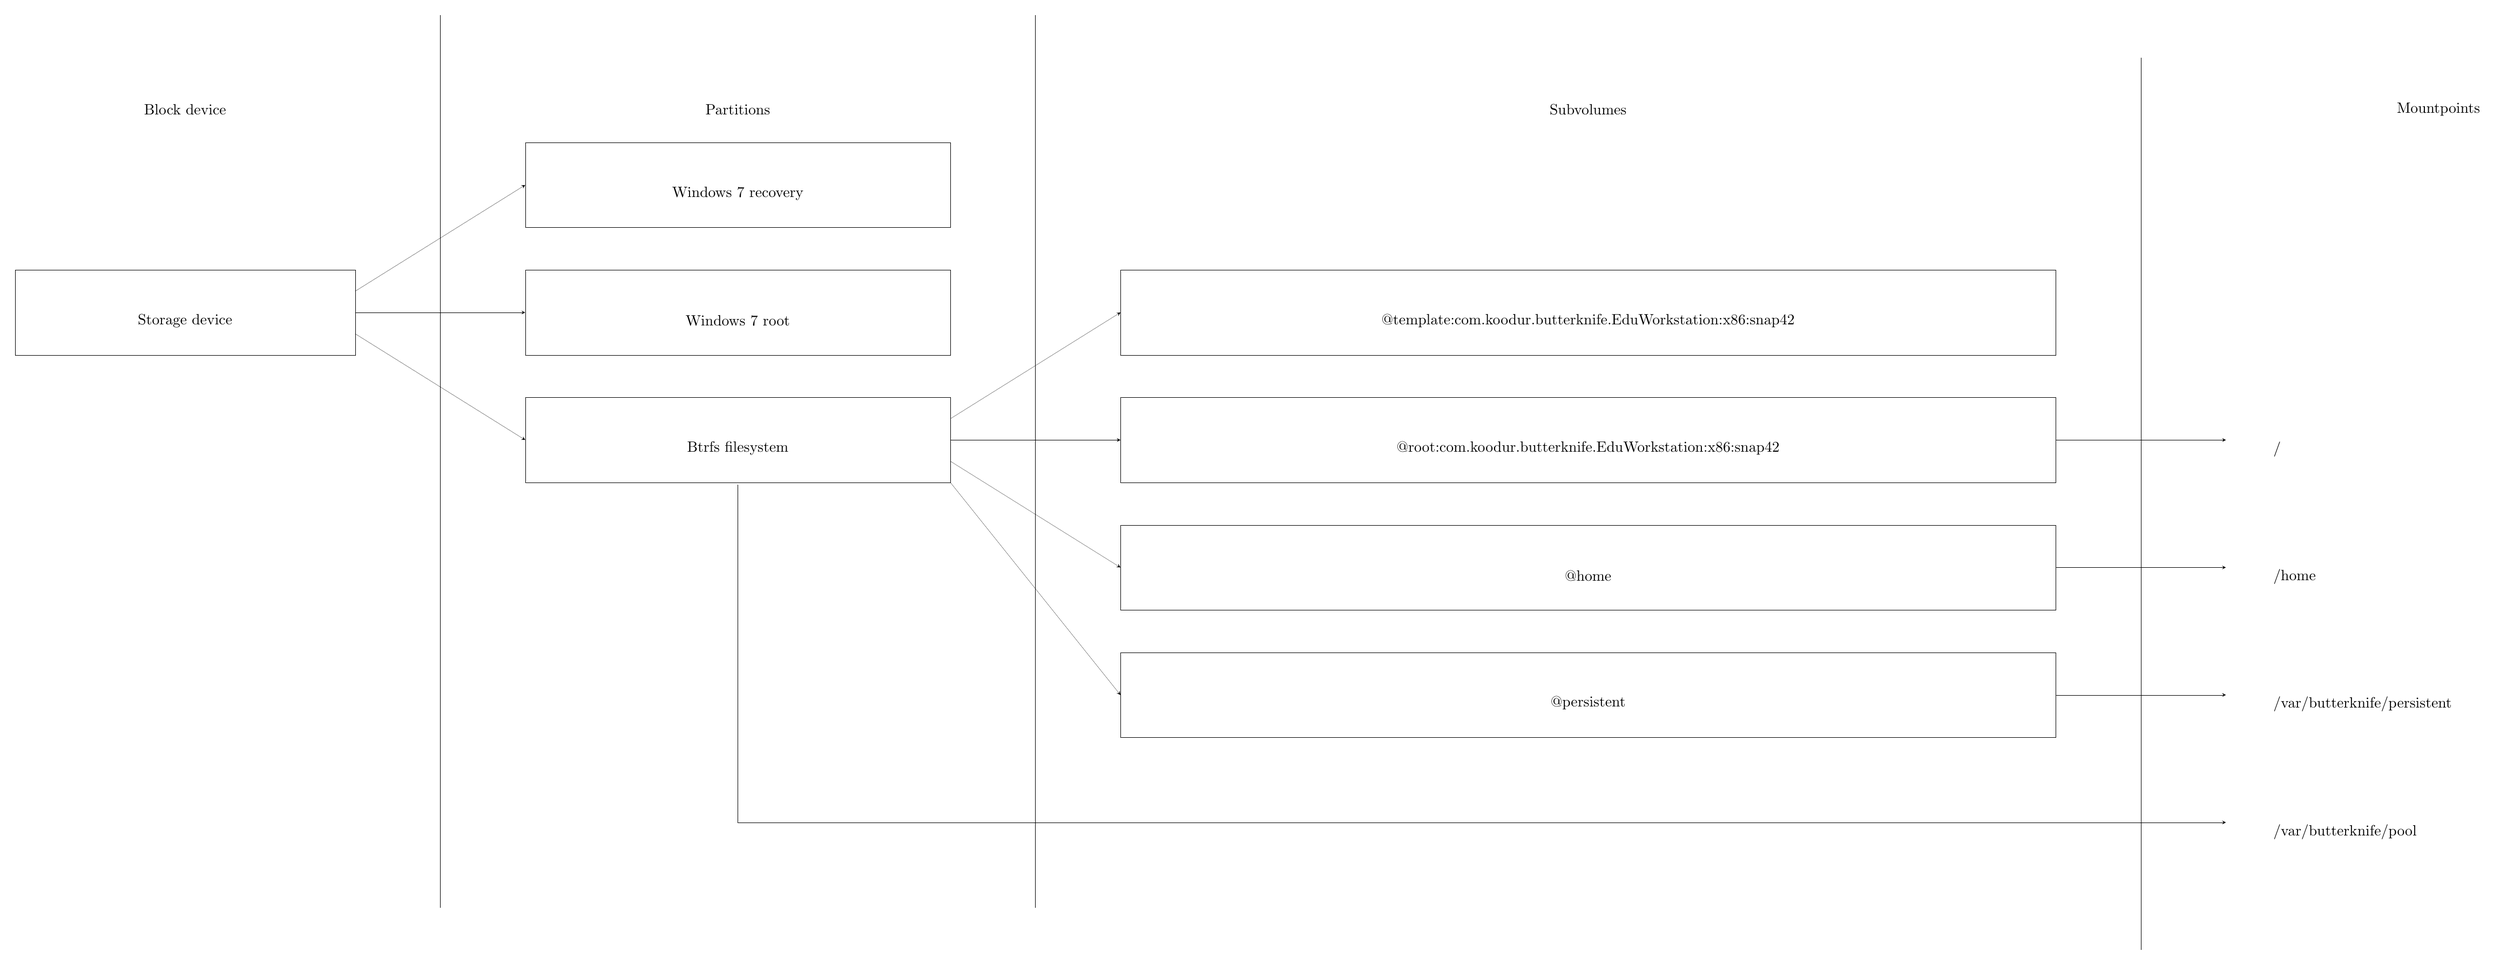
\begin{tikzpicture}
\pgftransformxscale{1.000000}
\pgftransformyscale{-1.000000}
\definecolor{dialinecolor}{rgb}{0.000000, 0.000000, 0.000000}
\pgfsetstrokecolor{dialinecolor}
\definecolor{dialinecolor}{rgb}{1.000000, 1.000000, 1.000000}
\pgfsetfillcolor{dialinecolor}
\definecolor{dialinecolor}{rgb}{1.000000, 1.000000, 1.000000}
\pgfsetfillcolor{dialinecolor}
\fill (27.000000\du,7.000000\du)--(27.000000\du,9.000000\du)--(49.000000\du,9.000000\du)--(49.000000\du,7.000000\du)--cycle;
\pgfsetlinewidth{0.100000\du}
\pgfsetdash{}{0pt}
\pgfsetdash{}{0pt}
\pgfsetmiterjoin
\definecolor{dialinecolor}{rgb}{0.000000, 0.000000, 0.000000}
\pgfsetstrokecolor{dialinecolor}
\draw (27.000000\du,7.000000\du)--(27.000000\du,9.000000\du)--(49.000000\du,9.000000\du)--(49.000000\du,7.000000\du)--cycle;
% setfont left to latex
\definecolor{dialinecolor}{rgb}{0.000000, 0.000000, 0.000000}
\pgfsetstrokecolor{dialinecolor}
\node at (38.000000\du,8.195000\du){@template:com.koodur.butterknife.EduWorkstation:x86:snap42};
\definecolor{dialinecolor}{rgb}{1.000000, 1.000000, 1.000000}
\pgfsetfillcolor{dialinecolor}
\fill (27.000000\du,10.000000\du)--(27.000000\du,12.000000\du)--(49.000000\du,12.000000\du)--(49.000000\du,10.000000\du)--cycle;
\pgfsetlinewidth{0.100000\du}
\pgfsetdash{}{0pt}
\pgfsetdash{}{0pt}
\pgfsetmiterjoin
\definecolor{dialinecolor}{rgb}{0.000000, 0.000000, 0.000000}
\pgfsetstrokecolor{dialinecolor}
\draw (27.000000\du,10.000000\du)--(27.000000\du,12.000000\du)--(49.000000\du,12.000000\du)--(49.000000\du,10.000000\du)--cycle;
% setfont left to latex
\definecolor{dialinecolor}{rgb}{0.000000, 0.000000, 0.000000}
\pgfsetstrokecolor{dialinecolor}
\node at (38.000000\du,11.195000\du){@root:com.koodur.butterknife.EduWorkstation:x86:snap42};
\definecolor{dialinecolor}{rgb}{1.000000, 1.000000, 1.000000}
\pgfsetfillcolor{dialinecolor}
\fill (27.000000\du,13.000000\du)--(27.000000\du,15.000000\du)--(49.000000\du,15.000000\du)--(49.000000\du,13.000000\du)--cycle;
\pgfsetlinewidth{0.100000\du}
\pgfsetdash{}{0pt}
\pgfsetdash{}{0pt}
\pgfsetmiterjoin
\definecolor{dialinecolor}{rgb}{0.000000, 0.000000, 0.000000}
\pgfsetstrokecolor{dialinecolor}
\draw (27.000000\du,13.000000\du)--(27.000000\du,15.000000\du)--(49.000000\du,15.000000\du)--(49.000000\du,13.000000\du)--cycle;
% setfont left to latex
\definecolor{dialinecolor}{rgb}{0.000000, 0.000000, 0.000000}
\pgfsetstrokecolor{dialinecolor}
\node at (38.000000\du,14.195000\du){@home};
\definecolor{dialinecolor}{rgb}{1.000000, 1.000000, 1.000000}
\pgfsetfillcolor{dialinecolor}
\fill (27.000000\du,16.000000\du)--(27.000000\du,18.000000\du)--(49.000000\du,18.000000\du)--(49.000000\du,16.000000\du)--cycle;
\pgfsetlinewidth{0.100000\du}
\pgfsetdash{}{0pt}
\pgfsetdash{}{0pt}
\pgfsetmiterjoin
\definecolor{dialinecolor}{rgb}{0.000000, 0.000000, 0.000000}
\pgfsetstrokecolor{dialinecolor}
\draw (27.000000\du,16.000000\du)--(27.000000\du,18.000000\du)--(49.000000\du,18.000000\du)--(49.000000\du,16.000000\du)--cycle;
% setfont left to latex
\definecolor{dialinecolor}{rgb}{0.000000, 0.000000, 0.000000}
\pgfsetstrokecolor{dialinecolor}
\node at (38.000000\du,17.195000\du){@persistent};
\pgfsetlinewidth{0.100000\du}
\pgfsetdash{}{0pt}
\pgfsetdash{}{0pt}
\pgfsetbuttcap
{
\definecolor{dialinecolor}{rgb}{0.000000, 0.000000, 0.000000}
\pgfsetfillcolor{dialinecolor}
% was here!!!
\pgfsetarrowsend{stealth}
\definecolor{dialinecolor}{rgb}{0.000000, 0.000000, 0.000000}
\pgfsetstrokecolor{dialinecolor}
\draw (49.000000\du,11.000000\du)--(53.000000\du,11.000000\du);
}
\pgfsetlinewidth{0.100000\du}
\pgfsetdash{}{0pt}
\pgfsetdash{}{0pt}
\pgfsetbuttcap
{
\definecolor{dialinecolor}{rgb}{0.000000, 0.000000, 0.000000}
\pgfsetfillcolor{dialinecolor}
% was here!!!
\pgfsetarrowsend{stealth}
\definecolor{dialinecolor}{rgb}{0.000000, 0.000000, 0.000000}
\pgfsetstrokecolor{dialinecolor}
\draw (49.000000\du,14.000000\du)--(53.000000\du,14.000000\du);
}
\pgfsetlinewidth{0.100000\du}
\pgfsetdash{}{0pt}
\pgfsetdash{}{0pt}
\pgfsetbuttcap
{
\definecolor{dialinecolor}{rgb}{0.000000, 0.000000, 0.000000}
\pgfsetfillcolor{dialinecolor}
% was here!!!
\pgfsetarrowsend{stealth}
\definecolor{dialinecolor}{rgb}{0.000000, 0.000000, 0.000000}
\pgfsetstrokecolor{dialinecolor}
\draw (49.000000\du,17.000000\du)--(53.000000\du,17.000000\du);
}
% setfont left to latex
\definecolor{dialinecolor}{rgb}{0.000000, 0.000000, 0.000000}
\pgfsetstrokecolor{dialinecolor}
\node[anchor=west] at (54.000000\du,14.221250\du){/home};
% setfont left to latex
\definecolor{dialinecolor}{rgb}{0.000000, 0.000000, 0.000000}
\pgfsetstrokecolor{dialinecolor}
\node[anchor=west] at (54.000000\du,17.221250\du){/var/butterknife/persistent};
% setfont left to latex
\definecolor{dialinecolor}{rgb}{0.000000, 0.000000, 0.000000}
\pgfsetstrokecolor{dialinecolor}
\node[anchor=west] at (54.000000\du,11.221250\du){/};
% setfont left to latex
\definecolor{dialinecolor}{rgb}{0.000000, 0.000000, 0.000000}
\pgfsetstrokecolor{dialinecolor}
\node[anchor=west] at (54.000000\du,20.221250\du){/var/butterknife/pool};
\definecolor{dialinecolor}{rgb}{1.000000, 1.000000, 1.000000}
\pgfsetfillcolor{dialinecolor}
\fill (1.000000\du,7.000000\du)--(1.000000\du,9.000000\du)--(9.000000\du,9.000000\du)--(9.000000\du,7.000000\du)--cycle;
\pgfsetlinewidth{0.100000\du}
\pgfsetdash{}{0pt}
\pgfsetdash{}{0pt}
\pgfsetmiterjoin
\definecolor{dialinecolor}{rgb}{0.000000, 0.000000, 0.000000}
\pgfsetstrokecolor{dialinecolor}
\draw (1.000000\du,7.000000\du)--(1.000000\du,9.000000\du)--(9.000000\du,9.000000\du)--(9.000000\du,7.000000\du)--cycle;
% setfont left to latex
\definecolor{dialinecolor}{rgb}{0.000000, 0.000000, 0.000000}
\pgfsetstrokecolor{dialinecolor}
\node at (5.000000\du,8.195000\du){Storage device};
\definecolor{dialinecolor}{rgb}{1.000000, 1.000000, 1.000000}
\pgfsetfillcolor{dialinecolor}
\fill (13.000000\du,4.000000\du)--(13.000000\du,6.000000\du)--(23.000000\du,6.000000\du)--(23.000000\du,4.000000\du)--cycle;
\pgfsetlinewidth{0.100000\du}
\pgfsetdash{}{0pt}
\pgfsetdash{}{0pt}
\pgfsetmiterjoin
\definecolor{dialinecolor}{rgb}{0.000000, 0.000000, 0.000000}
\pgfsetstrokecolor{dialinecolor}
\draw (13.000000\du,4.000000\du)--(13.000000\du,6.000000\du)--(23.000000\du,6.000000\du)--(23.000000\du,4.000000\du)--cycle;
% setfont left to latex
\definecolor{dialinecolor}{rgb}{0.000000, 0.000000, 0.000000}
\pgfsetstrokecolor{dialinecolor}
\node at (18.000000\du,5.195000\du){Windows 7 recovery};
\definecolor{dialinecolor}{rgb}{1.000000, 1.000000, 1.000000}
\pgfsetfillcolor{dialinecolor}
\fill (13.000000\du,10.000000\du)--(13.000000\du,12.000000\du)--(23.000000\du,12.000000\du)--(23.000000\du,10.000000\du)--cycle;
\pgfsetlinewidth{0.100000\du}
\pgfsetdash{}{0pt}
\pgfsetdash{}{0pt}
\pgfsetmiterjoin
\definecolor{dialinecolor}{rgb}{0.000000, 0.000000, 0.000000}
\pgfsetstrokecolor{dialinecolor}
\draw (13.000000\du,10.000000\du)--(13.000000\du,12.000000\du)--(23.000000\du,12.000000\du)--(23.000000\du,10.000000\du)--cycle;
% setfont left to latex
\definecolor{dialinecolor}{rgb}{0.000000, 0.000000, 0.000000}
\pgfsetstrokecolor{dialinecolor}
\node at (18.000000\du,11.195000\du){Btrfs filesystem};
\definecolor{dialinecolor}{rgb}{1.000000, 1.000000, 1.000000}
\pgfsetfillcolor{dialinecolor}
\fill (13.000000\du,7.000000\du)--(13.000000\du,9.000000\du)--(23.000000\du,9.000000\du)--(23.000000\du,7.000000\du)--cycle;
\pgfsetlinewidth{0.100000\du}
\pgfsetdash{}{0pt}
\pgfsetdash{}{0pt}
\pgfsetmiterjoin
\definecolor{dialinecolor}{rgb}{0.000000, 0.000000, 0.000000}
\pgfsetstrokecolor{dialinecolor}
\draw (13.000000\du,7.000000\du)--(13.000000\du,9.000000\du)--(23.000000\du,9.000000\du)--(23.000000\du,7.000000\du)--cycle;
% setfont left to latex
\definecolor{dialinecolor}{rgb}{0.000000, 0.000000, 0.000000}
\pgfsetstrokecolor{dialinecolor}
\node at (18.000000\du,8.195000\du){Windows 7 root};
\pgfsetlinewidth{0.100000\du}
\pgfsetdash{}{0pt}
\pgfsetdash{}{0pt}
\pgfsetbuttcap
{
\definecolor{dialinecolor}{rgb}{0.000000, 0.000000, 0.000000}
\pgfsetfillcolor{dialinecolor}
% was here!!!
\pgfsetarrowsend{stealth}
\definecolor{dialinecolor}{rgb}{0.000000, 0.000000, 0.000000}
\pgfsetstrokecolor{dialinecolor}
\draw (23.000000\du,10.500000\du)--(27.000000\du,8.000000\du);
}
\pgfsetlinewidth{0.100000\du}
\pgfsetdash{}{0pt}
\pgfsetdash{}{0pt}
\pgfsetbuttcap
{
\definecolor{dialinecolor}{rgb}{0.000000, 0.000000, 0.000000}
\pgfsetfillcolor{dialinecolor}
% was here!!!
\pgfsetarrowsend{stealth}
\definecolor{dialinecolor}{rgb}{0.000000, 0.000000, 0.000000}
\pgfsetstrokecolor{dialinecolor}
\draw (23.000000\du,11.000000\du)--(27.000000\du,11.000000\du);
}
\pgfsetlinewidth{0.100000\du}
\pgfsetdash{}{0pt}
\pgfsetdash{}{0pt}
\pgfsetbuttcap
{
\definecolor{dialinecolor}{rgb}{0.000000, 0.000000, 0.000000}
\pgfsetfillcolor{dialinecolor}
% was here!!!
\pgfsetarrowsend{stealth}
\definecolor{dialinecolor}{rgb}{0.000000, 0.000000, 0.000000}
\pgfsetstrokecolor{dialinecolor}
\draw (23.000000\du,11.500000\du)--(27.000000\du,14.000000\du);
}
\pgfsetlinewidth{0.100000\du}
\pgfsetdash{}{0pt}
\pgfsetdash{}{0pt}
\pgfsetbuttcap
{
\definecolor{dialinecolor}{rgb}{0.000000, 0.000000, 0.000000}
\pgfsetfillcolor{dialinecolor}
% was here!!!
\pgfsetarrowsend{stealth}
\definecolor{dialinecolor}{rgb}{0.000000, 0.000000, 0.000000}
\pgfsetstrokecolor{dialinecolor}
\draw (9.000000\du,7.500000\du)--(13.000000\du,5.000000\du);
}
\pgfsetlinewidth{0.100000\du}
\pgfsetdash{}{0pt}
\pgfsetdash{}{0pt}
\pgfsetbuttcap
{
\definecolor{dialinecolor}{rgb}{0.000000, 0.000000, 0.000000}
\pgfsetfillcolor{dialinecolor}
% was here!!!
\pgfsetarrowsend{stealth}
\definecolor{dialinecolor}{rgb}{0.000000, 0.000000, 0.000000}
\pgfsetstrokecolor{dialinecolor}
\draw (9.000000\du,8.000000\du)--(13.000000\du,8.000000\du);
}
\pgfsetlinewidth{0.100000\du}
\pgfsetdash{}{0pt}
\pgfsetdash{}{0pt}
\pgfsetbuttcap
{
\definecolor{dialinecolor}{rgb}{0.000000, 0.000000, 0.000000}
\pgfsetfillcolor{dialinecolor}
% was here!!!
\pgfsetarrowsend{stealth}
\definecolor{dialinecolor}{rgb}{0.000000, 0.000000, 0.000000}
\pgfsetstrokecolor{dialinecolor}
\draw (9.000000\du,8.500000\du)--(13.000000\du,11.000000\du);
}
\pgfsetlinewidth{0.100000\du}
\pgfsetdash{}{0pt}
\pgfsetdash{}{0pt}
\pgfsetbuttcap
{
\definecolor{dialinecolor}{rgb}{0.000000, 0.000000, 0.000000}
\pgfsetfillcolor{dialinecolor}
% was here!!!
\pgfsetarrowsend{stealth}
\definecolor{dialinecolor}{rgb}{0.000000, 0.000000, 0.000000}
\pgfsetstrokecolor{dialinecolor}
\draw (23.000000\du,12.000000\du)--(27.000000\du,17.000000\du);
}
% setfont left to latex
\definecolor{dialinecolor}{rgb}{0.000000, 0.000000, 0.000000}
\pgfsetstrokecolor{dialinecolor}
\node at (5.000000\du,3.221250\du){Block device};
% setfont left to latex
\definecolor{dialinecolor}{rgb}{0.000000, 0.000000, 0.000000}
\pgfsetstrokecolor{dialinecolor}
\node at (18.000000\du,3.221250\du){Partitions};
% setfont left to latex
\definecolor{dialinecolor}{rgb}{0.000000, 0.000000, 0.000000}
\pgfsetstrokecolor{dialinecolor}
\node at (38.000000\du,3.221250\du){Subvolumes};
\pgfsetlinewidth{0.100000\du}
\pgfsetdash{{\pgflinewidth}{0.200000\du}}{0cm}
\pgfsetdash{{\pgflinewidth}{0.200000\du}}{0cm}
\pgfsetbuttcap
{
\definecolor{dialinecolor}{rgb}{0.000000, 0.000000, 0.000000}
\pgfsetfillcolor{dialinecolor}
% was here!!!
\definecolor{dialinecolor}{rgb}{0.000000, 0.000000, 0.000000}
\pgfsetstrokecolor{dialinecolor}
\draw (11.000000\du,1.000000\du)--(11.000000\du,22.000000\du);
}
\pgfsetlinewidth{0.100000\du}
\pgfsetdash{{\pgflinewidth}{0.200000\du}}{0cm}
\pgfsetdash{{\pgflinewidth}{0.200000\du}}{0cm}
\pgfsetbuttcap
{
\definecolor{dialinecolor}{rgb}{0.000000, 0.000000, 0.000000}
\pgfsetfillcolor{dialinecolor}
% was here!!!
\definecolor{dialinecolor}{rgb}{0.000000, 0.000000, 0.000000}
\pgfsetstrokecolor{dialinecolor}
\draw (25.000000\du,1.000000\du)--(25.000000\du,22.000000\du);
}
\pgfsetlinewidth{0.100000\du}
\pgfsetdash{{\pgflinewidth}{0.200000\du}}{0cm}
\pgfsetdash{{\pgflinewidth}{0.200000\du}}{0cm}
\pgfsetbuttcap
{
\definecolor{dialinecolor}{rgb}{0.000000, 0.000000, 0.000000}
\pgfsetfillcolor{dialinecolor}
% was here!!!
\definecolor{dialinecolor}{rgb}{0.000000, 0.000000, 0.000000}
\pgfsetstrokecolor{dialinecolor}
\draw (51.000000\du,2.000000\du)--(51.000000\du,23.000000\du);
}
% setfont left to latex
\definecolor{dialinecolor}{rgb}{0.000000, 0.000000, 0.000000}
\pgfsetstrokecolor{dialinecolor}
\node at (58.000000\du,3.221250\du){Mountpoints};
\pgfsetlinewidth{0.100000\du}
\pgfsetdash{}{0pt}
\pgfsetdash{}{0pt}
\pgfsetmiterjoin
\pgfsetbuttcap
{
\definecolor{dialinecolor}{rgb}{0.000000, 0.000000, 0.000000}
\pgfsetfillcolor{dialinecolor}
% was here!!!
\pgfsetarrowsend{stealth}
{\pgfsetcornersarced{\pgfpoint{0.000000\du}{0.000000\du}}\definecolor{dialinecolor}{rgb}{0.000000, 0.000000, 0.000000}
\pgfsetstrokecolor{dialinecolor}
\draw (18.000000\du,12.048096\du)--(18.000000\du,20.000000\du)--(53.000000\du,20.000000\du);
}}
\end{tikzpicture}
}
\caption{Pooled partitioning}
\label{fig:pooled-partitioning}
\end{figure}


\subsection{Benchmarks}

As root filesystem contains numerous small files significant
slowdown was observed is spinning disk was used on the either
side.
The throughput averaged ~37MB/s while
streaming Ubuntu root filesystem to/from
Western Digital WD40EFRX without using encryption or compression.
Using SSD-s on both ends averaged around 100MB/s
due to gigabit ethernet used for benchmarking.


\section{Conclusions and Future work}

\subsection{Conclusions}

The implementation exceeds rather than  the needs of educational 



\subsection{Future work}

\subsubsection{BitTorrent integration}


\begin{figure}[!htb]
\centering
\scalebox{0.5}{% Graphic for TeX using PGF
% Title: /home/lauri/Projektid/msc-thesis/dia/butterknife-usecase-bittorrent.dia
% Creator: Dia v0.97.2
% CreationDate: Sun Mar 15 12:50:40 2015
% For: lauri
% \usepackage{tikz}
% The following commands are not supported in PSTricks at present
% We define them conditionally, so when they are implemented,
% this pgf file will use them.
\ifx\du\undefined
  \newlength{\du}
\fi
\setlength{\du}{15\unitlength}
\begin{tikzpicture}
\pgftransformxscale{1.000000}
\pgftransformyscale{-1.000000}
\definecolor{dialinecolor}{rgb}{0.000000, 0.000000, 0.000000}
\pgfsetstrokecolor{dialinecolor}
\definecolor{dialinecolor}{rgb}{1.000000, 1.000000, 1.000000}
\pgfsetfillcolor{dialinecolor}
\pgfsetlinewidth{0.100000\du}
\pgfsetdash{}{0pt}
\pgfsetdash{}{0pt}
\pgfsetbuttcap
\pgfsetmiterjoin
\pgfsetlinewidth{0.001000\du}
\pgfsetbuttcap
\pgfsetmiterjoin
\pgfsetdash{}{0pt}
\definecolor{dialinecolor}{rgb}{0.788235, 0.788235, 0.713726}
\pgfsetfillcolor{dialinecolor}
\pgfpathmoveto{\pgfpoint{2.593877\du}{13.817207\du}}
\pgfpathlineto{\pgfpoint{2.998822\du}{13.439344\du}}
\pgfpathlineto{\pgfpoint{6.022370\du}{13.439344\du}}
\pgfpathlineto{\pgfpoint{5.618070\du}{13.817207\du}}
\pgfpathlineto{\pgfpoint{2.593877\du}{13.817207\du}}
\pgfusepath{fill}
\pgfsetbuttcap
\pgfsetmiterjoin
\pgfsetdash{}{0pt}
\definecolor{dialinecolor}{rgb}{0.286275, 0.286275, 0.211765}
\pgfsetstrokecolor{dialinecolor}
\pgfpathmoveto{\pgfpoint{2.593877\du}{13.817207\du}}
\pgfpathlineto{\pgfpoint{2.998822\du}{13.439344\du}}
\pgfpathlineto{\pgfpoint{6.022370\du}{13.439344\du}}
\pgfpathlineto{\pgfpoint{5.618070\du}{13.817207\du}}
\pgfpathlineto{\pgfpoint{2.593877\du}{13.817207\du}}
\pgfusepath{stroke}
\pgfsetbuttcap
\pgfsetmiterjoin
\pgfsetdash{}{0pt}
\definecolor{dialinecolor}{rgb}{0.717647, 0.717647, 0.615686}
\pgfsetfillcolor{dialinecolor}
\pgfpathmoveto{\pgfpoint{2.593877\du}{13.817207\du}}
\pgfpathlineto{\pgfpoint{5.618070\du}{13.817207\du}}
\pgfpathlineto{\pgfpoint{5.618070\du}{14.385290\du}}
\pgfpathlineto{\pgfpoint{2.593877\du}{14.385290\du}}
\pgfpathlineto{\pgfpoint{2.593877\du}{13.817207\du}}
\pgfusepath{fill}
\pgfsetbuttcap
\pgfsetmiterjoin
\pgfsetdash{}{0pt}
\definecolor{dialinecolor}{rgb}{0.286275, 0.286275, 0.211765}
\pgfsetstrokecolor{dialinecolor}
\pgfpathmoveto{\pgfpoint{2.593877\du}{13.817207\du}}
\pgfpathlineto{\pgfpoint{5.618070\du}{13.817207\du}}
\pgfpathlineto{\pgfpoint{5.618070\du}{14.385290\du}}
\pgfpathlineto{\pgfpoint{2.593877\du}{14.385290\du}}
\pgfpathlineto{\pgfpoint{2.593877\du}{13.817207\du}}
\pgfusepath{stroke}
\pgfsetbuttcap
\pgfsetmiterjoin
\pgfsetdash{}{0pt}
\definecolor{dialinecolor}{rgb}{0.478431, 0.478431, 0.352941}
\pgfsetfillcolor{dialinecolor}
\pgfpathmoveto{\pgfpoint{5.618070\du}{14.385290\du}}
\pgfpathlineto{\pgfpoint{6.022370\du}{13.982280\du}}
\pgfpathlineto{\pgfpoint{6.022370\du}{13.439344\du}}
\pgfpathlineto{\pgfpoint{5.618070\du}{13.817207\du}}
\pgfpathlineto{\pgfpoint{5.618070\du}{14.385290\du}}
\pgfusepath{fill}
\pgfsetbuttcap
\pgfsetmiterjoin
\pgfsetdash{}{0pt}
\definecolor{dialinecolor}{rgb}{0.286275, 0.286275, 0.211765}
\pgfsetstrokecolor{dialinecolor}
\pgfpathmoveto{\pgfpoint{5.618070\du}{14.385290\du}}
\pgfpathlineto{\pgfpoint{6.022370\du}{13.982280\du}}
\pgfpathlineto{\pgfpoint{6.022370\du}{13.439344\du}}
\pgfpathlineto{\pgfpoint{5.618070\du}{13.817207\du}}
\pgfpathlineto{\pgfpoint{5.618070\du}{14.385290\du}}
\pgfusepath{stroke}
\pgfsetbuttcap
\pgfsetmiterjoin
\pgfsetdash{}{0pt}
\definecolor{dialinecolor}{rgb}{0.000000, 0.000000, 0.000000}
\pgfsetfillcolor{dialinecolor}
\pgfpathmoveto{\pgfpoint{2.689954\du}{13.746277\du}}
\pgfpathlineto{\pgfpoint{2.998822\du}{13.439344\du}}
\pgfpathlineto{\pgfpoint{5.950795\du}{13.439344\du}}
\pgfpathlineto{\pgfpoint{5.641283\du}{13.746277\du}}
\pgfpathlineto{\pgfpoint{2.689954\du}{13.746277\du}}
\pgfusepath{fill}
\pgfsetbuttcap
\pgfsetmiterjoin
\pgfsetdash{}{0pt}
\definecolor{dialinecolor}{rgb}{0.000000, 0.000000, 0.000000}
\pgfsetstrokecolor{dialinecolor}
\pgfpathmoveto{\pgfpoint{2.689954\du}{13.746277\du}}
\pgfpathlineto{\pgfpoint{2.998822\du}{13.439344\du}}
\pgfpathlineto{\pgfpoint{5.950795\du}{13.439344\du}}
\pgfpathlineto{\pgfpoint{5.641283\du}{13.746277\du}}
\pgfpathlineto{\pgfpoint{2.689954\du}{13.746277\du}}
\pgfusepath{stroke}
\pgfsetbuttcap
\pgfsetmiterjoin
\pgfsetdash{}{0pt}
\definecolor{dialinecolor}{rgb}{0.788235, 0.788235, 0.713726}
\pgfsetfillcolor{dialinecolor}
\pgfpathmoveto{\pgfpoint{2.593877\du}{11.306933\du}}
\pgfpathlineto{\pgfpoint{2.927892\du}{11.000000\du}}
\pgfpathlineto{\pgfpoint{5.950795\du}{11.000000\du}}
\pgfpathlineto{\pgfpoint{5.618070\du}{11.306933\du}}
\pgfpathlineto{\pgfpoint{2.593877\du}{11.306933\du}}
\pgfusepath{fill}
\pgfsetbuttcap
\pgfsetmiterjoin
\pgfsetdash{}{0pt}
\definecolor{dialinecolor}{rgb}{0.286275, 0.286275, 0.211765}
\pgfsetstrokecolor{dialinecolor}
\pgfpathmoveto{\pgfpoint{2.593877\du}{11.306933\du}}
\pgfpathlineto{\pgfpoint{2.927892\du}{11.000000\du}}
\pgfpathlineto{\pgfpoint{5.950795\du}{11.000000\du}}
\pgfpathlineto{\pgfpoint{5.618070\du}{11.306933\du}}
\pgfpathlineto{\pgfpoint{2.593877\du}{11.306933\du}}
\pgfusepath{stroke}
\pgfsetbuttcap
\pgfsetmiterjoin
\pgfsetdash{}{0pt}
\definecolor{dialinecolor}{rgb}{0.717647, 0.717647, 0.615686}
\pgfsetfillcolor{dialinecolor}
\pgfpathmoveto{\pgfpoint{2.593877\du}{11.306933\du}}
\pgfpathlineto{\pgfpoint{5.640638\du}{11.306933\du}}
\pgfpathlineto{\pgfpoint{5.640638\du}{13.699205\du}}
\pgfpathlineto{\pgfpoint{2.593877\du}{13.699205\du}}
\pgfpathlineto{\pgfpoint{2.593877\du}{11.306933\du}}
\pgfusepath{fill}
\pgfsetbuttcap
\pgfsetmiterjoin
\pgfsetdash{}{0pt}
\definecolor{dialinecolor}{rgb}{0.286275, 0.286275, 0.211765}
\pgfsetstrokecolor{dialinecolor}
\pgfpathmoveto{\pgfpoint{2.593877\du}{11.306933\du}}
\pgfpathlineto{\pgfpoint{5.639993\du}{11.306933\du}}
\pgfpathlineto{\pgfpoint{5.639993\du}{13.697915\du}}
\pgfpathlineto{\pgfpoint{2.593877\du}{13.697915\du}}
\pgfpathlineto{\pgfpoint{2.593877\du}{11.306933\du}}
\pgfusepath{stroke}
\pgfsetbuttcap
\pgfsetmiterjoin
\pgfsetdash{}{0pt}
\definecolor{dialinecolor}{rgb}{1.000000, 1.000000, 1.000000}
\pgfsetfillcolor{dialinecolor}
\pgfpathmoveto{\pgfpoint{2.857607\du}{11.615156\du}}
\pgfpathlineto{\pgfpoint{5.380132\du}{11.615156\du}}
\pgfpathlineto{\pgfpoint{5.380132\du}{13.462557\du}}
\pgfpathlineto{\pgfpoint{2.857607\du}{13.462557\du}}
\pgfpathlineto{\pgfpoint{2.857607\du}{11.615156\du}}
\pgfusepath{fill}
\pgfsetbuttcap
\pgfsetmiterjoin
\pgfsetdash{}{0pt}
\definecolor{dialinecolor}{rgb}{0.286275, 0.286275, 0.211765}
\pgfsetstrokecolor{dialinecolor}
\pgfpathmoveto{\pgfpoint{2.857607\du}{11.615156\du}}
\pgfpathlineto{\pgfpoint{5.379487\du}{11.615156\du}}
\pgfpathlineto{\pgfpoint{5.379487\du}{13.461267\du}}
\pgfpathlineto{\pgfpoint{2.857607\du}{13.461267\du}}
\pgfpathlineto{\pgfpoint{2.857607\du}{11.615156\du}}
\pgfusepath{stroke}
\pgfsetbuttcap
\pgfsetmiterjoin
\pgfsetdash{}{0pt}
\definecolor{dialinecolor}{rgb}{0.478431, 0.478431, 0.352941}
\pgfsetfillcolor{dialinecolor}
\pgfpathmoveto{\pgfpoint{5.618070\du}{13.674057\du}}
\pgfpathlineto{\pgfpoint{5.950795\du}{13.343266\du}}
\pgfpathlineto{\pgfpoint{5.950795\du}{11.000000\du}}
\pgfpathlineto{\pgfpoint{5.618070\du}{11.306933\du}}
\pgfpathlineto{\pgfpoint{5.618070\du}{13.674057\du}}
\pgfusepath{fill}
\pgfsetbuttcap
\pgfsetmiterjoin
\pgfsetdash{}{0pt}
\definecolor{dialinecolor}{rgb}{0.286275, 0.286275, 0.211765}
\pgfsetstrokecolor{dialinecolor}
\pgfpathmoveto{\pgfpoint{5.618070\du}{13.674057\du}}
\pgfpathlineto{\pgfpoint{5.950795\du}{13.343266\du}}
\pgfpathlineto{\pgfpoint{5.950795\du}{11.000000\du}}
\pgfpathlineto{\pgfpoint{5.618070\du}{11.306933\du}}
\pgfpathlineto{\pgfpoint{5.618070\du}{13.674057\du}}
\pgfusepath{stroke}
\pgfsetbuttcap
\pgfsetmiterjoin
\pgfsetdash{}{0pt}
\definecolor{dialinecolor}{rgb}{0.788235, 0.788235, 0.713726}
\pgfsetfillcolor{dialinecolor}
\pgfpathmoveto{\pgfpoint{2.000000\du}{14.858586\du}}
\pgfpathlineto{\pgfpoint{2.475875\du}{14.267289\du}}
\pgfpathlineto{\pgfpoint{5.759284\du}{14.267289\du}}
\pgfpathlineto{\pgfpoint{5.284054\du}{14.858586\du}}
\pgfpathlineto{\pgfpoint{2.000000\du}{14.858586\du}}
\pgfusepath{fill}
\pgfsetbuttcap
\pgfsetmiterjoin
\pgfsetdash{}{0pt}
\definecolor{dialinecolor}{rgb}{0.286275, 0.286275, 0.211765}
\pgfsetstrokecolor{dialinecolor}
\pgfpathmoveto{\pgfpoint{2.003224\du}{14.854717\du}}
\pgfpathlineto{\pgfpoint{2.475875\du}{14.267289\du}}
\pgfpathlineto{\pgfpoint{5.759284\du}{14.267289\du}}
\pgfpathlineto{\pgfpoint{5.284054\du}{14.858586\du}}
\pgfpathlineto{\pgfpoint{2.003224\du}{14.858586\du}}
\pgfusepath{stroke}
\pgfsetbuttcap
\pgfsetmiterjoin
\pgfsetdash{}{0pt}
\definecolor{dialinecolor}{rgb}{0.478431, 0.478431, 0.352941}
\pgfsetfillcolor{dialinecolor}
\pgfpathmoveto{\pgfpoint{5.284054\du}{14.977878\du}}
\pgfpathlineto{\pgfpoint{5.759284\du}{14.480079\du}}
\pgfpathlineto{\pgfpoint{5.759284\du}{14.267289\du}}
\pgfpathlineto{\pgfpoint{5.284054\du}{14.858586\du}}
\pgfpathlineto{\pgfpoint{5.284054\du}{14.977878\du}}
\pgfusepath{fill}
\pgfsetbuttcap
\pgfsetmiterjoin
\pgfsetdash{}{0pt}
\definecolor{dialinecolor}{rgb}{0.286275, 0.286275, 0.211765}
\pgfsetstrokecolor{dialinecolor}
\pgfpathmoveto{\pgfpoint{5.285989\du}{14.974653\du}}
\pgfpathlineto{\pgfpoint{5.759284\du}{14.480079\du}}
\pgfpathlineto{\pgfpoint{5.759284\du}{14.267289\du}}
\pgfpathlineto{\pgfpoint{5.284054\du}{14.858586\du}}
\pgfpathlineto{\pgfpoint{5.284054\du}{14.974653\du}}
\pgfusepath{stroke}
\pgfsetbuttcap
\pgfsetmiterjoin
\pgfsetdash{}{0pt}
\definecolor{dialinecolor}{rgb}{0.717647, 0.717647, 0.615686}
\pgfsetfillcolor{dialinecolor}
\pgfpathmoveto{\pgfpoint{2.000000\du}{14.858586\du}}
\pgfpathlineto{\pgfpoint{5.284054\du}{14.858586\du}}
\pgfpathlineto{\pgfpoint{5.284054\du}{14.977878\du}}
\pgfpathlineto{\pgfpoint{2.000000\du}{14.977878\du}}
\pgfpathlineto{\pgfpoint{2.000000\du}{14.858586\du}}
\pgfusepath{fill}
\pgfsetbuttcap
\pgfsetmiterjoin
\pgfsetdash{}{0pt}
\definecolor{dialinecolor}{rgb}{0.286275, 0.286275, 0.211765}
\pgfsetstrokecolor{dialinecolor}
\pgfpathmoveto{\pgfpoint{2.003224\du}{14.858586\du}}
\pgfpathlineto{\pgfpoint{5.284054\du}{14.858586\du}}
\pgfpathlineto{\pgfpoint{5.284054\du}{14.974653\du}}
\pgfusepath{stroke}
% setfont left to latex
\definecolor{dialinecolor}{rgb}{0.000000, 0.000000, 0.000000}
\pgfsetstrokecolor{dialinecolor}
\node at (4.000000\du,16.221250\du){x86 workstation};
\pgfsetlinewidth{0.100000\du}
\pgfsetdash{}{0pt}
\pgfsetdash{}{0pt}
\pgfsetbuttcap
\pgfsetmiterjoin
\pgfsetlinewidth{0.001000\du}
\pgfsetbuttcap
\pgfsetmiterjoin
\pgfsetdash{}{0pt}
\definecolor{dialinecolor}{rgb}{0.647059, 0.647059, 0.521569}
\pgfsetfillcolor{dialinecolor}
\pgfpathmoveto{\pgfpoint{17.000000\du}{21.123976\du}}
\pgfpathlineto{\pgfpoint{16.997269\du}{21.089022\du}}
\pgfpathlineto{\pgfpoint{16.989623\du}{21.054615\du}}
\pgfpathlineto{\pgfpoint{16.976516\du}{21.020208\du}}
\pgfpathlineto{\pgfpoint{16.958493\du}{20.986346\du}}
\pgfpathlineto{\pgfpoint{16.936100\du}{20.952485\du}}
\pgfpathlineto{\pgfpoint{16.908247\du}{20.919170\du}}
\pgfpathlineto{\pgfpoint{16.875478\du}{20.886401\du}}
\pgfpathlineto{\pgfpoint{16.837794\du}{20.854178\du}}
\pgfpathlineto{\pgfpoint{16.795194\du}{20.822501\du}}
\pgfpathlineto{\pgfpoint{16.748225\du}{20.792463\du}}
\pgfpathlineto{\pgfpoint{16.696887\du}{20.762425\du}}
\pgfpathlineto{\pgfpoint{16.641726\du}{20.732933\du}}
\pgfpathlineto{\pgfpoint{16.581103\du}{20.705079\du}}
\pgfpathlineto{\pgfpoint{16.517204\du}{20.678318\du}}
\pgfpathlineto{\pgfpoint{16.449481\du}{20.652649\du}}
\pgfpathlineto{\pgfpoint{16.377389\du}{20.628072\du}}
\pgfpathlineto{\pgfpoint{16.302567\du}{20.605134\du}}
\pgfpathlineto{\pgfpoint{16.223921\du}{20.583288\du}}
\pgfpathlineto{\pgfpoint{16.142545\du}{20.563080\du}}
\pgfpathlineto{\pgfpoint{16.057346\du}{20.543965\du}}
\pgfpathlineto{\pgfpoint{15.970508\du}{20.525942\du}}
\pgfpathlineto{\pgfpoint{15.880393\du}{20.510104\du}}
\pgfpathlineto{\pgfpoint{15.788094\du}{20.494812\du}}
\pgfpathlineto{\pgfpoint{15.694702\du}{20.482250\du}}
\pgfpathlineto{\pgfpoint{15.598580\du}{20.471327\du}}
\pgfpathlineto{\pgfpoint{15.500819\du}{20.462043\du}}
\pgfpathlineto{\pgfpoint{15.402512\du}{20.453850\du}}
\pgfpathlineto{\pgfpoint{15.302567\du}{20.448389\du}}
\pgfpathlineto{\pgfpoint{15.202075\du}{20.443474\du}}
\pgfpathlineto{\pgfpoint{15.101038\du}{20.440197\du}}
\pgfpathlineto{\pgfpoint{15.000000\du}{20.440197\du}}
\pgfpathlineto{\pgfpoint{15.000000\du}{20.440197\du}}
\pgfpathlineto{\pgfpoint{14.898416\du}{20.440197\du}}
\pgfpathlineto{\pgfpoint{14.797378\du}{20.443474\du}}
\pgfpathlineto{\pgfpoint{14.696887\du}{20.448389\du}}
\pgfpathlineto{\pgfpoint{14.596942\du}{20.453850\du}}
\pgfpathlineto{\pgfpoint{14.498635\du}{20.462043\du}}
\pgfpathlineto{\pgfpoint{14.400874\du}{20.471327\du}}
\pgfpathlineto{\pgfpoint{14.305298\du}{20.482250\du}}
\pgfpathlineto{\pgfpoint{14.211360\du}{20.494812\du}}
\pgfpathlineto{\pgfpoint{14.119061\du}{20.510104\du}}
\pgfpathlineto{\pgfpoint{14.028946\du}{20.525942\du}}
\pgfpathlineto{\pgfpoint{13.942108\du}{20.543965\du}}
\pgfpathlineto{\pgfpoint{13.857455\du}{20.563080\du}}
\pgfpathlineto{\pgfpoint{13.776079\du}{20.583288\du}}
\pgfpathlineto{\pgfpoint{13.697433\du}{20.605134\du}}
\pgfpathlineto{\pgfpoint{13.622064\du}{20.628072\du}}
\pgfpathlineto{\pgfpoint{13.549973\du}{20.652649\du}}
\pgfpathlineto{\pgfpoint{13.482796\du}{20.678318\du}}
\pgfpathlineto{\pgfpoint{13.418351\du}{20.705079\du}}
\pgfpathlineto{\pgfpoint{13.358274\du}{20.732933\du}}
\pgfpathlineto{\pgfpoint{13.302567\du}{20.762425\du}}
\pgfpathlineto{\pgfpoint{13.251229\du}{20.792463\du}}
\pgfpathlineto{\pgfpoint{13.204260\du}{20.822501\du}}
\pgfpathlineto{\pgfpoint{13.161660\du}{20.854178\du}}
\pgfpathlineto{\pgfpoint{13.123976\du}{20.886401\du}}
\pgfpathlineto{\pgfpoint{13.091207\du}{20.919170\du}}
\pgfpathlineto{\pgfpoint{13.063353\du}{20.952485\du}}
\pgfpathlineto{\pgfpoint{13.040961\du}{20.986346\du}}
\pgfpathlineto{\pgfpoint{13.022938\du}{21.020208\du}}
\pgfpathlineto{\pgfpoint{13.009831\du}{21.054615\du}}
\pgfpathlineto{\pgfpoint{13.002731\du}{21.089022\du}}
\pgfpathlineto{\pgfpoint{13.000000\du}{21.123976\du}}
\pgfpathlineto{\pgfpoint{13.000000\du}{21.123976\du}}
\pgfpathlineto{\pgfpoint{13.002731\du}{21.158930\du}}
\pgfpathlineto{\pgfpoint{13.009831\du}{21.192791\du}}
\pgfpathlineto{\pgfpoint{13.022938\du}{21.227744\du}}
\pgfpathlineto{\pgfpoint{13.040961\du}{21.261606\du}}
\pgfpathlineto{\pgfpoint{13.063353\du}{21.295467\du}}
\pgfpathlineto{\pgfpoint{13.091207\du}{21.328782\du}}
\pgfpathlineto{\pgfpoint{13.123976\du}{21.361551\du}}
\pgfpathlineto{\pgfpoint{13.161660\du}{21.393774\du}}
\pgfpathlineto{\pgfpoint{13.204260\du}{21.424904\du}}
\pgfpathlineto{\pgfpoint{13.251229\du}{21.455489\du}}
\pgfpathlineto{\pgfpoint{13.302567\du}{21.485527\du}}
\pgfpathlineto{\pgfpoint{13.358274\du}{21.515019\du}}
\pgfpathlineto{\pgfpoint{13.418351\du}{21.542873\du}}
\pgfpathlineto{\pgfpoint{13.482796\du}{21.569634\du}}
\pgfpathlineto{\pgfpoint{13.549973\du}{21.595303\du}}
\pgfpathlineto{\pgfpoint{13.622064\du}{21.619880\du}}
\pgfpathlineto{\pgfpoint{13.697433\du}{21.642818\du}}
\pgfpathlineto{\pgfpoint{13.776079\du}{21.664664\du}}
\pgfpathlineto{\pgfpoint{13.857455\du}{21.684872\du}}
\pgfpathlineto{\pgfpoint{13.942108\du}{21.703987\du}}
\pgfpathlineto{\pgfpoint{14.028946\du}{21.722010\du}}
\pgfpathlineto{\pgfpoint{14.119061\du}{21.737848\du}}
\pgfpathlineto{\pgfpoint{14.211360\du}{21.752594\du}}
\pgfpathlineto{\pgfpoint{14.305298\du}{21.765702\du}}
\pgfpathlineto{\pgfpoint{14.400874\du}{21.776625\du}}
\pgfpathlineto{\pgfpoint{14.498635\du}{21.785909\du}}
\pgfpathlineto{\pgfpoint{14.596942\du}{21.793555\du}}
\pgfpathlineto{\pgfpoint{14.696887\du}{21.799563\du}}
\pgfpathlineto{\pgfpoint{14.797378\du}{21.803932\du}}
\pgfpathlineto{\pgfpoint{14.898416\du}{21.807209\du}}
\pgfpathlineto{\pgfpoint{15.000000\du}{21.807755\du}}
\pgfpathlineto{\pgfpoint{15.000000\du}{21.807755\du}}
\pgfpathlineto{\pgfpoint{15.101038\du}{21.807209\du}}
\pgfpathlineto{\pgfpoint{15.202075\du}{21.803932\du}}
\pgfpathlineto{\pgfpoint{15.302567\du}{21.799563\du}}
\pgfpathlineto{\pgfpoint{15.402512\du}{21.793555\du}}
\pgfpathlineto{\pgfpoint{15.500819\du}{21.785909\du}}
\pgfpathlineto{\pgfpoint{15.598580\du}{21.776625\du}}
\pgfpathlineto{\pgfpoint{15.694702\du}{21.765702\du}}
\pgfpathlineto{\pgfpoint{15.788094\du}{21.752594\du}}
\pgfpathlineto{\pgfpoint{15.880393\du}{21.737848\du}}
\pgfpathlineto{\pgfpoint{15.970508\du}{21.722010\du}}
\pgfpathlineto{\pgfpoint{16.057346\du}{21.703987\du}}
\pgfpathlineto{\pgfpoint{16.142545\du}{21.684872\du}}
\pgfpathlineto{\pgfpoint{16.223921\du}{21.664664\du}}
\pgfpathlineto{\pgfpoint{16.302567\du}{21.642818\du}}
\pgfpathlineto{\pgfpoint{16.377389\du}{21.619880\du}}
\pgfpathlineto{\pgfpoint{16.449481\du}{21.595303\du}}
\pgfpathlineto{\pgfpoint{16.517204\du}{21.569634\du}}
\pgfpathlineto{\pgfpoint{16.581103\du}{21.542873\du}}
\pgfpathlineto{\pgfpoint{16.641726\du}{21.515019\du}}
\pgfpathlineto{\pgfpoint{16.696887\du}{21.485527\du}}
\pgfpathlineto{\pgfpoint{16.748225\du}{21.455489\du}}
\pgfpathlineto{\pgfpoint{16.795194\du}{21.424904\du}}
\pgfpathlineto{\pgfpoint{16.837794\du}{21.393774\du}}
\pgfpathlineto{\pgfpoint{16.875478\du}{21.361551\du}}
\pgfpathlineto{\pgfpoint{16.908247\du}{21.328782\du}}
\pgfpathlineto{\pgfpoint{16.936100\du}{21.295467\du}}
\pgfpathlineto{\pgfpoint{16.958493\du}{21.261606\du}}
\pgfpathlineto{\pgfpoint{16.976516\du}{21.227744\du}}
\pgfpathlineto{\pgfpoint{16.989623\du}{21.192791\du}}
\pgfpathlineto{\pgfpoint{16.997269\du}{21.158930\du}}
\pgfpathlineto{\pgfpoint{17.000000\du}{21.123976\du}}
\pgfusepath{fill}
\pgfsetbuttcap
\pgfsetmiterjoin
\pgfsetdash{}{0pt}
\definecolor{dialinecolor}{rgb}{0.286275, 0.286275, 0.211765}
\pgfsetstrokecolor{dialinecolor}
\pgfpathmoveto{\pgfpoint{16.976516\du}{21.113053\du}}
\pgfpathlineto{\pgfpoint{16.973785\du}{21.078099\du}}
\pgfpathlineto{\pgfpoint{16.966685\du}{21.044784\du}}
\pgfpathlineto{\pgfpoint{16.954123\du}{21.010923\du}}
\pgfpathlineto{\pgfpoint{16.936647\du}{20.977608\du}}
\pgfpathlineto{\pgfpoint{16.913162\du}{20.943747\du}}
\pgfpathlineto{\pgfpoint{16.884762\du}{20.911524\du}}
\pgfpathlineto{\pgfpoint{16.853632\du}{20.878755\du}}
\pgfpathlineto{\pgfpoint{16.815401\du}{20.848170\du}}
\pgfpathlineto{\pgfpoint{16.773348\du}{20.817040\du}}
\pgfpathlineto{\pgfpoint{16.726925\du}{20.786455\du}}
\pgfpathlineto{\pgfpoint{16.675587\du}{20.757510\du}}
\pgfpathlineto{\pgfpoint{16.620426\du}{20.728564\du}}
\pgfpathlineto{\pgfpoint{16.560896\du}{20.701256\du}}
\pgfpathlineto{\pgfpoint{16.498088\du}{20.673949\du}}
\pgfpathlineto{\pgfpoint{16.429274\du}{20.649372\du}}
\pgfpathlineto{\pgfpoint{16.357728\du}{20.625341\du}}
\pgfpathlineto{\pgfpoint{16.282906\du}{20.602403\du}}
\pgfpathlineto{\pgfpoint{16.205352\du}{20.581103\du}}
\pgfpathlineto{\pgfpoint{16.124522\du}{20.561442\du}}
\pgfpathlineto{\pgfpoint{16.040415\du}{20.542327\du}}
\pgfpathlineto{\pgfpoint{15.953031\du}{20.525396\du}}
\pgfpathlineto{\pgfpoint{15.864009\du}{20.509558\du}}
\pgfpathlineto{\pgfpoint{15.772256\du}{20.494812\du}}
\pgfpathlineto{\pgfpoint{15.679410\du}{20.482250\du}}
\pgfpathlineto{\pgfpoint{15.584380\du}{20.471327\du}}
\pgfpathlineto{\pgfpoint{15.486619\du}{20.462589\du}}
\pgfpathlineto{\pgfpoint{15.388859\du}{20.453850\du}}
\pgfpathlineto{\pgfpoint{15.289459\du}{20.448935\du}}
\pgfpathlineto{\pgfpoint{15.190060\du}{20.444566\du}}
\pgfpathlineto{\pgfpoint{15.088476\du}{20.441835\du}}
\pgfpathlineto{\pgfpoint{14.987985\du}{20.440197\du}}
\pgfpathlineto{\pgfpoint{14.987985\du}{20.440197\du}}
\pgfpathlineto{\pgfpoint{14.887493\du}{20.441835\du}}
\pgfpathlineto{\pgfpoint{14.787002\du}{20.444566\du}}
\pgfpathlineto{\pgfpoint{14.686510\du}{20.448935\du}}
\pgfpathlineto{\pgfpoint{14.588203\du}{20.453850\du}}
\pgfpathlineto{\pgfpoint{14.489896\du}{20.462589\du}}
\pgfpathlineto{\pgfpoint{14.392682\du}{20.471327\du}}
\pgfpathlineto{\pgfpoint{14.297105\du}{20.482250\du}}
\pgfpathlineto{\pgfpoint{14.203714\du}{20.494812\du}}
\pgfpathlineto{\pgfpoint{14.112507\du}{20.509558\du}}
\pgfpathlineto{\pgfpoint{14.023484\du}{20.525396\du}}
\pgfpathlineto{\pgfpoint{13.936100\du}{20.542327\du}}
\pgfpathlineto{\pgfpoint{13.851993\du}{20.561442\du}}
\pgfpathlineto{\pgfpoint{13.771709\du}{20.581103\du}}
\pgfpathlineto{\pgfpoint{13.693064\du}{20.602403\du}}
\pgfpathlineto{\pgfpoint{13.617695\du}{20.625341\du}}
\pgfpathlineto{\pgfpoint{13.546696\du}{20.649372\du}}
\pgfpathlineto{\pgfpoint{13.478973\du}{20.673949\du}}
\pgfpathlineto{\pgfpoint{13.416166\du}{20.701256\du}}
\pgfpathlineto{\pgfpoint{13.356090\du}{20.728564\du}}
\pgfpathlineto{\pgfpoint{13.300382\du}{20.757510\du}}
\pgfpathlineto{\pgfpoint{13.250137\du}{20.786455\du}}
\pgfpathlineto{\pgfpoint{13.203714\du}{20.817040\du}}
\pgfpathlineto{\pgfpoint{13.160568\du}{20.848170\du}}
\pgfpathlineto{\pgfpoint{13.123430\du}{20.878755\du}}
\pgfpathlineto{\pgfpoint{13.091207\du}{20.911524\du}}
\pgfpathlineto{\pgfpoint{13.063353\du}{20.943747\du}}
\pgfpathlineto{\pgfpoint{13.040415\du}{20.977608\du}}
\pgfpathlineto{\pgfpoint{13.022392\du}{21.010923\du}}
\pgfpathlineto{\pgfpoint{13.009831\du}{21.044784\du}}
\pgfpathlineto{\pgfpoint{13.002731\du}{21.078099\du}}
\pgfpathlineto{\pgfpoint{13.000000\du}{21.113053\du}}
\pgfpathlineto{\pgfpoint{13.000000\du}{21.113053\du}}
\pgfpathlineto{\pgfpoint{13.002731\du}{21.146914\du}}
\pgfpathlineto{\pgfpoint{13.009831\du}{21.180229\du}}
\pgfpathlineto{\pgfpoint{13.022392\du}{21.214637\du}}
\pgfpathlineto{\pgfpoint{13.040415\du}{21.247952\du}}
\pgfpathlineto{\pgfpoint{13.063353\du}{21.281267\du}}
\pgfpathlineto{\pgfpoint{13.091207\du}{21.314036\du}}
\pgfpathlineto{\pgfpoint{13.123430\du}{21.346259\du}}
\pgfpathlineto{\pgfpoint{13.160568\du}{21.377389\du}}
\pgfpathlineto{\pgfpoint{13.203714\du}{21.407974\du}}
\pgfpathlineto{\pgfpoint{13.250137\du}{21.439104\du}}
\pgfpathlineto{\pgfpoint{13.300382\du}{21.468596\du}}
\pgfpathlineto{\pgfpoint{13.356090\du}{21.496450\du}}
\pgfpathlineto{\pgfpoint{13.416166\du}{21.524304\du}}
\pgfpathlineto{\pgfpoint{13.478973\du}{21.551065\du}}
\pgfpathlineto{\pgfpoint{13.546696\du}{21.576188\du}}
\pgfpathlineto{\pgfpoint{13.617695\du}{21.600218\du}}
\pgfpathlineto{\pgfpoint{13.693064\du}{21.622611\du}}
\pgfpathlineto{\pgfpoint{13.771709\du}{21.644457\du}}
\pgfpathlineto{\pgfpoint{13.851993\du}{21.664118\du}}
\pgfpathlineto{\pgfpoint{13.936100\du}{21.683233\du}}
\pgfpathlineto{\pgfpoint{14.023484\du}{21.700710\du}}
\pgfpathlineto{\pgfpoint{14.112507\du}{21.716002\du}}
\pgfpathlineto{\pgfpoint{14.203714\du}{21.730202\du}}
\pgfpathlineto{\pgfpoint{14.297105\du}{21.742764\du}}
\pgfpathlineto{\pgfpoint{14.392682\du}{21.753687\du}}
\pgfpathlineto{\pgfpoint{14.489896\du}{21.762971\du}}
\pgfpathlineto{\pgfpoint{14.588203\du}{21.771163\du}}
\pgfpathlineto{\pgfpoint{14.686510\du}{21.776625\du}}
\pgfpathlineto{\pgfpoint{14.787002\du}{21.780994\du}}
\pgfpathlineto{\pgfpoint{14.887493\du}{21.783725\du}}
\pgfpathlineto{\pgfpoint{14.987985\du}{21.784817\du}}
\pgfpathlineto{\pgfpoint{14.987985\du}{21.784817\du}}
\pgfpathlineto{\pgfpoint{15.088476\du}{21.783725\du}}
\pgfpathlineto{\pgfpoint{15.190060\du}{21.780994\du}}
\pgfpathlineto{\pgfpoint{15.289459\du}{21.776625\du}}
\pgfpathlineto{\pgfpoint{15.388859\du}{21.771163\du}}
\pgfpathlineto{\pgfpoint{15.486619\du}{21.762971\du}}
\pgfpathlineto{\pgfpoint{15.584380\du}{21.753687\du}}
\pgfpathlineto{\pgfpoint{15.679410\du}{21.742764\du}}
\pgfpathlineto{\pgfpoint{15.772256\du}{21.730202\du}}
\pgfpathlineto{\pgfpoint{15.864009\du}{21.716002\du}}
\pgfpathlineto{\pgfpoint{15.953031\du}{21.700710\du}}
\pgfpathlineto{\pgfpoint{16.040415\du}{21.683233\du}}
\pgfpathlineto{\pgfpoint{16.124522\du}{21.664118\du}}
\pgfpathlineto{\pgfpoint{16.205352\du}{21.644457\du}}
\pgfpathlineto{\pgfpoint{16.282906\du}{21.622611\du}}
\pgfpathlineto{\pgfpoint{16.357728\du}{21.600218\du}}
\pgfpathlineto{\pgfpoint{16.429274\du}{21.576188\du}}
\pgfpathlineto{\pgfpoint{16.498088\du}{21.551065\du}}
\pgfpathlineto{\pgfpoint{16.560896\du}{21.524304\du}}
\pgfpathlineto{\pgfpoint{16.620426\du}{21.496450\du}}
\pgfpathlineto{\pgfpoint{16.675587\du}{21.468596\du}}
\pgfpathlineto{\pgfpoint{16.726925\du}{21.439104\du}}
\pgfpathlineto{\pgfpoint{16.773348\du}{21.407974\du}}
\pgfpathlineto{\pgfpoint{16.815401\du}{21.377389\du}}
\pgfpathlineto{\pgfpoint{16.853632\du}{21.346259\du}}
\pgfpathlineto{\pgfpoint{16.884762\du}{21.314036\du}}
\pgfpathlineto{\pgfpoint{16.913162\du}{21.281267\du}}
\pgfpathlineto{\pgfpoint{16.936647\du}{21.247952\du}}
\pgfpathlineto{\pgfpoint{16.954123\du}{21.214637\du}}
\pgfpathlineto{\pgfpoint{16.966685\du}{21.180229\du}}
\pgfpathlineto{\pgfpoint{16.973785\du}{21.146914\du}}
\pgfpathlineto{\pgfpoint{16.976516\du}{21.113053\du}}
\pgfusepath{stroke}
\pgfsetbuttcap
\pgfsetmiterjoin
\pgfsetdash{}{0pt}
\definecolor{dialinecolor}{rgb}{0.647059, 0.647059, 0.521569}
\pgfsetfillcolor{dialinecolor}
\pgfpathmoveto{\pgfpoint{13.000000\du}{19.695795\du}}
\pgfpathlineto{\pgfpoint{13.000000\du}{21.135991\du}}
\pgfpathlineto{\pgfpoint{16.976516\du}{21.135991\du}}
\pgfpathlineto{\pgfpoint{16.976516\du}{19.695795\du}}
\pgfpathlineto{\pgfpoint{13.000000\du}{19.695795\du}}
\pgfusepath{fill}
\pgfsetbuttcap
\pgfsetmiterjoin
\pgfsetdash{}{0pt}
\definecolor{dialinecolor}{rgb}{0.788235, 0.788235, 0.713726}
\pgfsetfillcolor{dialinecolor}
\pgfpathmoveto{\pgfpoint{17.000000\du}{19.683779\du}}
\pgfpathlineto{\pgfpoint{16.997269\du}{19.648280\du}}
\pgfpathlineto{\pgfpoint{16.989623\du}{19.613872\du}}
\pgfpathlineto{\pgfpoint{16.976516\du}{19.580011\du}}
\pgfpathlineto{\pgfpoint{16.958493\du}{19.546150\du}}
\pgfpathlineto{\pgfpoint{16.936100\du}{19.511742\du}}
\pgfpathlineto{\pgfpoint{16.908247\du}{19.478427\du}}
\pgfpathlineto{\pgfpoint{16.875478\du}{19.445112\du}}
\pgfpathlineto{\pgfpoint{16.837794\du}{19.413981\du}}
\pgfpathlineto{\pgfpoint{16.795194\du}{19.382851\du}}
\pgfpathlineto{\pgfpoint{16.748225\du}{19.351174\du}}
\pgfpathlineto{\pgfpoint{16.696887\du}{19.322228\du}}
\pgfpathlineto{\pgfpoint{16.641726\du}{19.292736\du}}
\pgfpathlineto{\pgfpoint{16.581103\du}{19.264336\du}}
\pgfpathlineto{\pgfpoint{16.517204\du}{19.238121\du}}
\pgfpathlineto{\pgfpoint{16.449481\du}{19.212452\du}}
\pgfpathlineto{\pgfpoint{16.377389\du}{19.187329\du}}
\pgfpathlineto{\pgfpoint{16.302567\du}{19.164391\du}}
\pgfpathlineto{\pgfpoint{16.223921\du}{19.143091\du}}
\pgfpathlineto{\pgfpoint{16.142545\du}{19.122338\du}}
\pgfpathlineto{\pgfpoint{16.057346\du}{19.103222\du}}
\pgfpathlineto{\pgfpoint{15.970508\du}{19.085745\du}}
\pgfpathlineto{\pgfpoint{15.880393\du}{19.069907\du}}
\pgfpathlineto{\pgfpoint{15.788094\du}{19.055161\du}}
\pgfpathlineto{\pgfpoint{15.694702\du}{19.042054\du}}
\pgfpathlineto{\pgfpoint{15.598580\du}{19.031131\du}}
\pgfpathlineto{\pgfpoint{15.500819\du}{19.021846\du}}
\pgfpathlineto{\pgfpoint{15.402512\du}{19.014200\du}}
\pgfpathlineto{\pgfpoint{15.302567\du}{19.008192\du}}
\pgfpathlineto{\pgfpoint{15.202075\du}{19.003277\du}}
\pgfpathlineto{\pgfpoint{15.101038\du}{19.000546\du}}
\pgfpathlineto{\pgfpoint{15.000000\du}{19.000000\du}}
\pgfpathlineto{\pgfpoint{15.000000\du}{19.000000\du}}
\pgfpathlineto{\pgfpoint{14.898416\du}{19.000546\du}}
\pgfpathlineto{\pgfpoint{14.797378\du}{19.003277\du}}
\pgfpathlineto{\pgfpoint{14.696887\du}{19.008192\du}}
\pgfpathlineto{\pgfpoint{14.596942\du}{19.014200\du}}
\pgfpathlineto{\pgfpoint{14.498635\du}{19.021846\du}}
\pgfpathlineto{\pgfpoint{14.400874\du}{19.031131\du}}
\pgfpathlineto{\pgfpoint{14.305298\du}{19.042054\du}}
\pgfpathlineto{\pgfpoint{14.211360\du}{19.055161\du}}
\pgfpathlineto{\pgfpoint{14.119061\du}{19.069907\du}}
\pgfpathlineto{\pgfpoint{14.028946\du}{19.085745\du}}
\pgfpathlineto{\pgfpoint{13.942108\du}{19.103222\du}}
\pgfpathlineto{\pgfpoint{13.857455\du}{19.122338\du}}
\pgfpathlineto{\pgfpoint{13.776079\du}{19.143091\du}}
\pgfpathlineto{\pgfpoint{13.697433\du}{19.164391\du}}
\pgfpathlineto{\pgfpoint{13.622064\du}{19.187329\du}}
\pgfpathlineto{\pgfpoint{13.549973\du}{19.212452\du}}
\pgfpathlineto{\pgfpoint{13.482796\du}{19.238121\du}}
\pgfpathlineto{\pgfpoint{13.418351\du}{19.264336\du}}
\pgfpathlineto{\pgfpoint{13.358274\du}{19.292736\du}}
\pgfpathlineto{\pgfpoint{13.302567\du}{19.322228\du}}
\pgfpathlineto{\pgfpoint{13.251229\du}{19.351174\du}}
\pgfpathlineto{\pgfpoint{13.204260\du}{19.382851\du}}
\pgfpathlineto{\pgfpoint{13.161660\du}{19.413981\du}}
\pgfpathlineto{\pgfpoint{13.123976\du}{19.445112\du}}
\pgfpathlineto{\pgfpoint{13.091207\du}{19.478427\du}}
\pgfpathlineto{\pgfpoint{13.063353\du}{19.511742\du}}
\pgfpathlineto{\pgfpoint{13.040961\du}{19.546150\du}}
\pgfpathlineto{\pgfpoint{13.022938\du}{19.580011\du}}
\pgfpathlineto{\pgfpoint{13.009831\du}{19.613872\du}}
\pgfpathlineto{\pgfpoint{13.002731\du}{19.648280\du}}
\pgfpathlineto{\pgfpoint{13.000000\du}{19.683779\du}}
\pgfpathlineto{\pgfpoint{13.000000\du}{19.683779\du}}
\pgfpathlineto{\pgfpoint{13.002731\du}{19.718187\du}}
\pgfpathlineto{\pgfpoint{13.009831\du}{19.753140\du}}
\pgfpathlineto{\pgfpoint{13.022938\du}{19.786455\du}}
\pgfpathlineto{\pgfpoint{13.040961\du}{19.821409\du}}
\pgfpathlineto{\pgfpoint{13.063353\du}{19.854724\du}}
\pgfpathlineto{\pgfpoint{13.091207\du}{19.888585\du}}
\pgfpathlineto{\pgfpoint{13.123976\du}{19.921354\du}}
\pgfpathlineto{\pgfpoint{13.161660\du}{19.953031\du}}
\pgfpathlineto{\pgfpoint{13.204260\du}{19.984708\du}}
\pgfpathlineto{\pgfpoint{13.251229\du}{20.015292\du}}
\pgfpathlineto{\pgfpoint{13.302567\du}{20.045330\du}}
\pgfpathlineto{\pgfpoint{13.358274\du}{20.074276\du}}
\pgfpathlineto{\pgfpoint{13.418351\du}{20.102130\du}}
\pgfpathlineto{\pgfpoint{13.482796\du}{20.128891\du}}
\pgfpathlineto{\pgfpoint{13.549973\du}{20.155106\du}}
\pgfpathlineto{\pgfpoint{13.622064\du}{20.179137\du}}
\pgfpathlineto{\pgfpoint{13.697433\du}{20.202622\du}}
\pgfpathlineto{\pgfpoint{13.776079\du}{20.224468\du}}
\pgfpathlineto{\pgfpoint{13.857455\du}{20.244675\du}}
\pgfpathlineto{\pgfpoint{13.942108\du}{20.263790\du}}
\pgfpathlineto{\pgfpoint{14.028946\du}{20.281813\du}}
\pgfpathlineto{\pgfpoint{14.119061\du}{20.297105\du}}
\pgfpathlineto{\pgfpoint{14.211360\du}{20.312398\du}}
\pgfpathlineto{\pgfpoint{14.305298\du}{20.324959\du}}
\pgfpathlineto{\pgfpoint{14.400874\du}{20.335882\du}}
\pgfpathlineto{\pgfpoint{14.498635\du}{20.345713\du}}
\pgfpathlineto{\pgfpoint{14.596942\du}{20.352813\du}}
\pgfpathlineto{\pgfpoint{14.696887\du}{20.359366\du}}
\pgfpathlineto{\pgfpoint{14.797378\du}{20.363736\du}}
\pgfpathlineto{\pgfpoint{14.898416\du}{20.366466\du}}
\pgfpathlineto{\pgfpoint{15.000000\du}{20.367559\du}}
\pgfpathlineto{\pgfpoint{15.000000\du}{20.367559\du}}
\pgfpathlineto{\pgfpoint{15.101038\du}{20.366466\du}}
\pgfpathlineto{\pgfpoint{15.202075\du}{20.363736\du}}
\pgfpathlineto{\pgfpoint{15.302567\du}{20.359366\du}}
\pgfpathlineto{\pgfpoint{15.402512\du}{20.352813\du}}
\pgfpathlineto{\pgfpoint{15.500819\du}{20.345713\du}}
\pgfpathlineto{\pgfpoint{15.598580\du}{20.335882\du}}
\pgfpathlineto{\pgfpoint{15.694702\du}{20.324959\du}}
\pgfpathlineto{\pgfpoint{15.788094\du}{20.312398\du}}
\pgfpathlineto{\pgfpoint{15.880393\du}{20.297105\du}}
\pgfpathlineto{\pgfpoint{15.970508\du}{20.281813\du}}
\pgfpathlineto{\pgfpoint{16.057346\du}{20.263790\du}}
\pgfpathlineto{\pgfpoint{16.142545\du}{20.244675\du}}
\pgfpathlineto{\pgfpoint{16.223921\du}{20.224468\du}}
\pgfpathlineto{\pgfpoint{16.302567\du}{20.202622\du}}
\pgfpathlineto{\pgfpoint{16.377389\du}{20.179137\du}}
\pgfpathlineto{\pgfpoint{16.449481\du}{20.155106\du}}
\pgfpathlineto{\pgfpoint{16.517204\du}{20.128891\du}}
\pgfpathlineto{\pgfpoint{16.581103\du}{20.102130\du}}
\pgfpathlineto{\pgfpoint{16.641726\du}{20.074276\du}}
\pgfpathlineto{\pgfpoint{16.696887\du}{20.045330\du}}
\pgfpathlineto{\pgfpoint{16.748225\du}{20.015292\du}}
\pgfpathlineto{\pgfpoint{16.795194\du}{19.984708\du}}
\pgfpathlineto{\pgfpoint{16.837794\du}{19.953031\du}}
\pgfpathlineto{\pgfpoint{16.875478\du}{19.921354\du}}
\pgfpathlineto{\pgfpoint{16.908247\du}{19.888585\du}}
\pgfpathlineto{\pgfpoint{16.936100\du}{19.854724\du}}
\pgfpathlineto{\pgfpoint{16.958493\du}{19.821409\du}}
\pgfpathlineto{\pgfpoint{16.976516\du}{19.786455\du}}
\pgfpathlineto{\pgfpoint{16.989623\du}{19.753140\du}}
\pgfpathlineto{\pgfpoint{16.997269\du}{19.718187\du}}
\pgfpathlineto{\pgfpoint{17.000000\du}{19.683779\du}}
\pgfusepath{fill}
\pgfsetbuttcap
\pgfsetmiterjoin
\pgfsetdash{}{0pt}
\definecolor{dialinecolor}{rgb}{0.286275, 0.286275, 0.211765}
\pgfsetstrokecolor{dialinecolor}
\pgfpathmoveto{\pgfpoint{16.976516\du}{19.672856\du}}
\pgfpathlineto{\pgfpoint{16.973785\du}{19.637903\du}}
\pgfpathlineto{\pgfpoint{16.966685\du}{19.604588\du}}
\pgfpathlineto{\pgfpoint{16.954123\du}{19.571273\du}}
\pgfpathlineto{\pgfpoint{16.936647\du}{19.537411\du}}
\pgfpathlineto{\pgfpoint{16.913162\du}{19.503004\du}}
\pgfpathlineto{\pgfpoint{16.884762\du}{19.470781\du}}
\pgfpathlineto{\pgfpoint{16.853632\du}{19.439650\du}}
\pgfpathlineto{\pgfpoint{16.815401\du}{19.407428\du}}
\pgfpathlineto{\pgfpoint{16.773348\du}{19.376843\du}}
\pgfpathlineto{\pgfpoint{16.726925\du}{19.345713\du}}
\pgfpathlineto{\pgfpoint{16.675587\du}{19.317313\du}}
\pgfpathlineto{\pgfpoint{16.620426\du}{19.288367\du}}
\pgfpathlineto{\pgfpoint{16.560896\du}{19.260513\du}}
\pgfpathlineto{\pgfpoint{16.498088\du}{19.234844\du}}
\pgfpathlineto{\pgfpoint{16.429274\du}{19.209175\du}}
\pgfpathlineto{\pgfpoint{16.357728\du}{19.185691\du}}
\pgfpathlineto{\pgfpoint{16.282906\du}{19.162753\du}}
\pgfpathlineto{\pgfpoint{16.205352\du}{19.140907\du}}
\pgfpathlineto{\pgfpoint{16.124522\du}{19.120699\du}}
\pgfpathlineto{\pgfpoint{16.040415\du}{19.102130\du}}
\pgfpathlineto{\pgfpoint{15.953031\du}{19.085199\du}}
\pgfpathlineto{\pgfpoint{15.864009\du}{19.069361\du}}
\pgfpathlineto{\pgfpoint{15.772256\du}{19.055161\du}}
\pgfpathlineto{\pgfpoint{15.679410\du}{19.042054\du}}
\pgfpathlineto{\pgfpoint{15.584380\du}{19.031131\du}}
\pgfpathlineto{\pgfpoint{15.486619\du}{19.021846\du}}
\pgfpathlineto{\pgfpoint{15.388859\du}{19.014200\du}}
\pgfpathlineto{\pgfpoint{15.289459\du}{19.008192\du}}
\pgfpathlineto{\pgfpoint{15.256144\du}{19.006554\du}}
\pgfpathlineto{\pgfpoint{14.719825\du}{19.006554\du}}
\pgfpathlineto{\pgfpoint{14.686510\du}{19.008192\du}}
\pgfpathlineto{\pgfpoint{14.588203\du}{19.014200\du}}
\pgfpathlineto{\pgfpoint{14.489896\du}{19.021846\du}}
\pgfpathlineto{\pgfpoint{14.392682\du}{19.031131\du}}
\pgfpathlineto{\pgfpoint{14.297105\du}{19.042054\du}}
\pgfpathlineto{\pgfpoint{14.203714\du}{19.055161\du}}
\pgfpathlineto{\pgfpoint{14.112507\du}{19.069361\du}}
\pgfpathlineto{\pgfpoint{14.023484\du}{19.085199\du}}
\pgfpathlineto{\pgfpoint{13.936100\du}{19.102130\du}}
\pgfpathlineto{\pgfpoint{13.851993\du}{19.120699\du}}
\pgfpathlineto{\pgfpoint{13.771709\du}{19.140907\du}}
\pgfpathlineto{\pgfpoint{13.693064\du}{19.162753\du}}
\pgfpathlineto{\pgfpoint{13.617695\du}{19.185691\du}}
\pgfpathlineto{\pgfpoint{13.546696\du}{19.209175\du}}
\pgfpathlineto{\pgfpoint{13.478973\du}{19.234844\du}}
\pgfpathlineto{\pgfpoint{13.416166\du}{19.260513\du}}
\pgfpathlineto{\pgfpoint{13.356090\du}{19.288367\du}}
\pgfpathlineto{\pgfpoint{13.300382\du}{19.317313\du}}
\pgfpathlineto{\pgfpoint{13.250137\du}{19.345713\du}}
\pgfpathlineto{\pgfpoint{13.203714\du}{19.376843\du}}
\pgfpathlineto{\pgfpoint{13.160568\du}{19.407428\du}}
\pgfpathlineto{\pgfpoint{13.123430\du}{19.439650\du}}
\pgfpathlineto{\pgfpoint{13.091207\du}{19.470781\du}}
\pgfpathlineto{\pgfpoint{13.063353\du}{19.503004\du}}
\pgfpathlineto{\pgfpoint{13.040415\du}{19.537411\du}}
\pgfpathlineto{\pgfpoint{13.022392\du}{19.571273\du}}
\pgfpathlineto{\pgfpoint{13.009831\du}{19.604588\du}}
\pgfpathlineto{\pgfpoint{13.002731\du}{19.637903\du}}
\pgfpathlineto{\pgfpoint{13.000000\du}{19.672856\du}}
\pgfpathlineto{\pgfpoint{13.000000\du}{19.672856\du}}
\pgfpathlineto{\pgfpoint{13.002731\du}{19.706171\du}}
\pgfpathlineto{\pgfpoint{13.009831\du}{19.740579\du}}
\pgfpathlineto{\pgfpoint{13.022392\du}{19.774440\du}}
\pgfpathlineto{\pgfpoint{13.040415\du}{19.807755\du}}
\pgfpathlineto{\pgfpoint{13.063353\du}{19.841070\du}}
\pgfpathlineto{\pgfpoint{13.091207\du}{19.873839\du}}
\pgfpathlineto{\pgfpoint{13.123430\du}{19.905516\du}}
\pgfpathlineto{\pgfpoint{13.160568\du}{19.937739\du}}
\pgfpathlineto{\pgfpoint{13.203714\du}{19.968323\du}}
\pgfpathlineto{\pgfpoint{13.250137\du}{19.998908\du}}
\pgfpathlineto{\pgfpoint{13.300382\du}{20.028400\du}}
\pgfpathlineto{\pgfpoint{13.356090\du}{20.056253\du}}
\pgfpathlineto{\pgfpoint{13.416166\du}{20.083561\du}}
\pgfpathlineto{\pgfpoint{13.478973\du}{20.110868\du}}
\pgfpathlineto{\pgfpoint{13.546696\du}{20.135991\du}}
\pgfpathlineto{\pgfpoint{13.617695\du}{20.159476\du}}
\pgfpathlineto{\pgfpoint{13.693064\du}{20.181868\du}}
\pgfpathlineto{\pgfpoint{13.771709\du}{20.203714\du}}
\pgfpathlineto{\pgfpoint{13.851993\du}{20.223375\du}}
\pgfpathlineto{\pgfpoint{13.936100\du}{20.242490\du}}
\pgfpathlineto{\pgfpoint{14.023484\du}{20.260513\du}}
\pgfpathlineto{\pgfpoint{14.112507\du}{20.274713\du}}
\pgfpathlineto{\pgfpoint{14.203714\du}{20.290005\du}}
\pgfpathlineto{\pgfpoint{14.297105\du}{20.302021\du}}
\pgfpathlineto{\pgfpoint{14.392682\du}{20.313490\du}}
\pgfpathlineto{\pgfpoint{14.489896\du}{20.323321\du}}
\pgfpathlineto{\pgfpoint{14.588203\du}{20.330967\du}}
\pgfpathlineto{\pgfpoint{14.686510\du}{20.336974\du}}
\pgfpathlineto{\pgfpoint{14.787002\du}{20.340797\du}}
\pgfpathlineto{\pgfpoint{14.887493\du}{20.342982\du}}
\pgfpathlineto{\pgfpoint{14.987985\du}{20.344620\du}}
\pgfpathlineto{\pgfpoint{14.987985\du}{20.344620\du}}
\pgfpathlineto{\pgfpoint{15.088476\du}{20.342982\du}}
\pgfpathlineto{\pgfpoint{15.190060\du}{20.340797\du}}
\pgfpathlineto{\pgfpoint{15.289459\du}{20.336974\du}}
\pgfpathlineto{\pgfpoint{15.388859\du}{20.330967\du}}
\pgfpathlineto{\pgfpoint{15.486619\du}{20.323321\du}}
\pgfpathlineto{\pgfpoint{15.584380\du}{20.313490\du}}
\pgfpathlineto{\pgfpoint{15.679410\du}{20.302021\du}}
\pgfpathlineto{\pgfpoint{15.772256\du}{20.290005\du}}
\pgfpathlineto{\pgfpoint{15.864009\du}{20.274713\du}}
\pgfpathlineto{\pgfpoint{15.953031\du}{20.260513\du}}
\pgfpathlineto{\pgfpoint{16.040415\du}{20.242490\du}}
\pgfpathlineto{\pgfpoint{16.124522\du}{20.223375\du}}
\pgfpathlineto{\pgfpoint{16.205352\du}{20.203714\du}}
\pgfpathlineto{\pgfpoint{16.282906\du}{20.181868\du}}
\pgfpathlineto{\pgfpoint{16.357728\du}{20.159476\du}}
\pgfpathlineto{\pgfpoint{16.429274\du}{20.135991\du}}
\pgfpathlineto{\pgfpoint{16.498088\du}{20.110868\du}}
\pgfpathlineto{\pgfpoint{16.560896\du}{20.083561\du}}
\pgfpathlineto{\pgfpoint{16.620426\du}{20.056253\du}}
\pgfpathlineto{\pgfpoint{16.675587\du}{20.028400\du}}
\pgfpathlineto{\pgfpoint{16.726925\du}{19.998908\du}}
\pgfpathlineto{\pgfpoint{16.773348\du}{19.968323\du}}
\pgfpathlineto{\pgfpoint{16.815401\du}{19.937739\du}}
\pgfpathlineto{\pgfpoint{16.853632\du}{19.905516\du}}
\pgfpathlineto{\pgfpoint{16.884762\du}{19.873839\du}}
\pgfpathlineto{\pgfpoint{16.913162\du}{19.841070\du}}
\pgfpathlineto{\pgfpoint{16.936647\du}{19.807755\du}}
\pgfpathlineto{\pgfpoint{16.954123\du}{19.774440\du}}
\pgfpathlineto{\pgfpoint{16.966685\du}{19.740579\du}}
\pgfpathlineto{\pgfpoint{16.973785\du}{19.706171\du}}
\pgfpathlineto{\pgfpoint{16.976516\du}{19.672856\du}}
\pgfusepath{stroke}
\pgfsetbuttcap
\pgfsetmiterjoin
\pgfsetdash{}{0pt}
\definecolor{dialinecolor}{rgb}{0.000000, 0.000000, 0.000000}
\pgfsetstrokecolor{dialinecolor}
\pgfpathmoveto{\pgfpoint{13.000000\du}{19.672856\du}}
\pgfpathlineto{\pgfpoint{13.000000\du}{21.111961\du}}
\pgfusepath{stroke}
\pgfsetbuttcap
\pgfsetmiterjoin
\pgfsetdash{}{0pt}
\definecolor{dialinecolor}{rgb}{0.000000, 0.000000, 0.000000}
\pgfsetstrokecolor{dialinecolor}
\pgfpathmoveto{\pgfpoint{16.976516\du}{19.672856\du}}
\pgfpathlineto{\pgfpoint{16.976516\du}{21.111961\du}}
\pgfusepath{stroke}
% setfont left to latex
\definecolor{dialinecolor}{rgb}{0.000000, 0.000000, 0.000000}
\pgfsetstrokecolor{dialinecolor}
\node at (15.000000\du,22.821250\du){Butterknife};
% setfont left to latex
\definecolor{dialinecolor}{rgb}{0.000000, 0.000000, 0.000000}
\pgfsetstrokecolor{dialinecolor}
\node at (15.000000\du,23.621250\du){server};
\pgfsetlinewidth{0.100000\du}
\pgfsetdash{}{0pt}
\pgfsetdash{}{0pt}
\pgfsetbuttcap
\pgfsetmiterjoin
\pgfsetlinewidth{0.001000\du}
\pgfsetbuttcap
\pgfsetmiterjoin
\pgfsetdash{}{0pt}
\definecolor{dialinecolor}{rgb}{0.788235, 0.788235, 0.713726}
\pgfsetfillcolor{dialinecolor}
\pgfpathmoveto{\pgfpoint{23.593877\du}{13.817207\du}}
\pgfpathlineto{\pgfpoint{23.998822\du}{13.439344\du}}
\pgfpathlineto{\pgfpoint{27.022370\du}{13.439344\du}}
\pgfpathlineto{\pgfpoint{26.618070\du}{13.817207\du}}
\pgfpathlineto{\pgfpoint{23.593877\du}{13.817207\du}}
\pgfusepath{fill}
\pgfsetbuttcap
\pgfsetmiterjoin
\pgfsetdash{}{0pt}
\definecolor{dialinecolor}{rgb}{0.286275, 0.286275, 0.211765}
\pgfsetstrokecolor{dialinecolor}
\pgfpathmoveto{\pgfpoint{23.593877\du}{13.817207\du}}
\pgfpathlineto{\pgfpoint{23.998822\du}{13.439344\du}}
\pgfpathlineto{\pgfpoint{27.022370\du}{13.439344\du}}
\pgfpathlineto{\pgfpoint{26.618070\du}{13.817207\du}}
\pgfpathlineto{\pgfpoint{23.593877\du}{13.817207\du}}
\pgfusepath{stroke}
\pgfsetbuttcap
\pgfsetmiterjoin
\pgfsetdash{}{0pt}
\definecolor{dialinecolor}{rgb}{0.717647, 0.717647, 0.615686}
\pgfsetfillcolor{dialinecolor}
\pgfpathmoveto{\pgfpoint{23.593877\du}{13.817207\du}}
\pgfpathlineto{\pgfpoint{26.618070\du}{13.817207\du}}
\pgfpathlineto{\pgfpoint{26.618070\du}{14.385290\du}}
\pgfpathlineto{\pgfpoint{23.593877\du}{14.385290\du}}
\pgfpathlineto{\pgfpoint{23.593877\du}{13.817207\du}}
\pgfusepath{fill}
\pgfsetbuttcap
\pgfsetmiterjoin
\pgfsetdash{}{0pt}
\definecolor{dialinecolor}{rgb}{0.286275, 0.286275, 0.211765}
\pgfsetstrokecolor{dialinecolor}
\pgfpathmoveto{\pgfpoint{23.593877\du}{13.817207\du}}
\pgfpathlineto{\pgfpoint{26.618070\du}{13.817207\du}}
\pgfpathlineto{\pgfpoint{26.618070\du}{14.385290\du}}
\pgfpathlineto{\pgfpoint{23.593877\du}{14.385290\du}}
\pgfpathlineto{\pgfpoint{23.593877\du}{13.817207\du}}
\pgfusepath{stroke}
\pgfsetbuttcap
\pgfsetmiterjoin
\pgfsetdash{}{0pt}
\definecolor{dialinecolor}{rgb}{0.478431, 0.478431, 0.352941}
\pgfsetfillcolor{dialinecolor}
\pgfpathmoveto{\pgfpoint{26.618070\du}{14.385290\du}}
\pgfpathlineto{\pgfpoint{27.022370\du}{13.982280\du}}
\pgfpathlineto{\pgfpoint{27.022370\du}{13.439344\du}}
\pgfpathlineto{\pgfpoint{26.618070\du}{13.817207\du}}
\pgfpathlineto{\pgfpoint{26.618070\du}{14.385290\du}}
\pgfusepath{fill}
\pgfsetbuttcap
\pgfsetmiterjoin
\pgfsetdash{}{0pt}
\definecolor{dialinecolor}{rgb}{0.286275, 0.286275, 0.211765}
\pgfsetstrokecolor{dialinecolor}
\pgfpathmoveto{\pgfpoint{26.618070\du}{14.385290\du}}
\pgfpathlineto{\pgfpoint{27.022370\du}{13.982280\du}}
\pgfpathlineto{\pgfpoint{27.022370\du}{13.439344\du}}
\pgfpathlineto{\pgfpoint{26.618070\du}{13.817207\du}}
\pgfpathlineto{\pgfpoint{26.618070\du}{14.385290\du}}
\pgfusepath{stroke}
\pgfsetbuttcap
\pgfsetmiterjoin
\pgfsetdash{}{0pt}
\definecolor{dialinecolor}{rgb}{0.000000, 0.000000, 0.000000}
\pgfsetfillcolor{dialinecolor}
\pgfpathmoveto{\pgfpoint{23.689954\du}{13.746277\du}}
\pgfpathlineto{\pgfpoint{23.998822\du}{13.439344\du}}
\pgfpathlineto{\pgfpoint{26.950795\du}{13.439344\du}}
\pgfpathlineto{\pgfpoint{26.641283\du}{13.746277\du}}
\pgfpathlineto{\pgfpoint{23.689954\du}{13.746277\du}}
\pgfusepath{fill}
\pgfsetbuttcap
\pgfsetmiterjoin
\pgfsetdash{}{0pt}
\definecolor{dialinecolor}{rgb}{0.000000, 0.000000, 0.000000}
\pgfsetstrokecolor{dialinecolor}
\pgfpathmoveto{\pgfpoint{23.689954\du}{13.746277\du}}
\pgfpathlineto{\pgfpoint{23.998822\du}{13.439344\du}}
\pgfpathlineto{\pgfpoint{26.950795\du}{13.439344\du}}
\pgfpathlineto{\pgfpoint{26.641283\du}{13.746277\du}}
\pgfpathlineto{\pgfpoint{23.689954\du}{13.746277\du}}
\pgfusepath{stroke}
\pgfsetbuttcap
\pgfsetmiterjoin
\pgfsetdash{}{0pt}
\definecolor{dialinecolor}{rgb}{0.788235, 0.788235, 0.713726}
\pgfsetfillcolor{dialinecolor}
\pgfpathmoveto{\pgfpoint{23.593877\du}{11.306933\du}}
\pgfpathlineto{\pgfpoint{23.927892\du}{11.000000\du}}
\pgfpathlineto{\pgfpoint{26.950795\du}{11.000000\du}}
\pgfpathlineto{\pgfpoint{26.618070\du}{11.306933\du}}
\pgfpathlineto{\pgfpoint{23.593877\du}{11.306933\du}}
\pgfusepath{fill}
\pgfsetbuttcap
\pgfsetmiterjoin
\pgfsetdash{}{0pt}
\definecolor{dialinecolor}{rgb}{0.286275, 0.286275, 0.211765}
\pgfsetstrokecolor{dialinecolor}
\pgfpathmoveto{\pgfpoint{23.593877\du}{11.306933\du}}
\pgfpathlineto{\pgfpoint{23.927892\du}{11.000000\du}}
\pgfpathlineto{\pgfpoint{26.950795\du}{11.000000\du}}
\pgfpathlineto{\pgfpoint{26.618070\du}{11.306933\du}}
\pgfpathlineto{\pgfpoint{23.593877\du}{11.306933\du}}
\pgfusepath{stroke}
\pgfsetbuttcap
\pgfsetmiterjoin
\pgfsetdash{}{0pt}
\definecolor{dialinecolor}{rgb}{0.717647, 0.717647, 0.615686}
\pgfsetfillcolor{dialinecolor}
\pgfpathmoveto{\pgfpoint{23.593877\du}{11.306933\du}}
\pgfpathlineto{\pgfpoint{26.640638\du}{11.306933\du}}
\pgfpathlineto{\pgfpoint{26.640638\du}{13.699205\du}}
\pgfpathlineto{\pgfpoint{23.593877\du}{13.699205\du}}
\pgfpathlineto{\pgfpoint{23.593877\du}{11.306933\du}}
\pgfusepath{fill}
\pgfsetbuttcap
\pgfsetmiterjoin
\pgfsetdash{}{0pt}
\definecolor{dialinecolor}{rgb}{0.286275, 0.286275, 0.211765}
\pgfsetstrokecolor{dialinecolor}
\pgfpathmoveto{\pgfpoint{23.593877\du}{11.306933\du}}
\pgfpathlineto{\pgfpoint{26.639993\du}{11.306933\du}}
\pgfpathlineto{\pgfpoint{26.639993\du}{13.697915\du}}
\pgfpathlineto{\pgfpoint{23.593877\du}{13.697915\du}}
\pgfpathlineto{\pgfpoint{23.593877\du}{11.306933\du}}
\pgfusepath{stroke}
\pgfsetbuttcap
\pgfsetmiterjoin
\pgfsetdash{}{0pt}
\definecolor{dialinecolor}{rgb}{1.000000, 1.000000, 1.000000}
\pgfsetfillcolor{dialinecolor}
\pgfpathmoveto{\pgfpoint{23.857607\du}{11.615156\du}}
\pgfpathlineto{\pgfpoint{26.380132\du}{11.615156\du}}
\pgfpathlineto{\pgfpoint{26.380132\du}{13.462557\du}}
\pgfpathlineto{\pgfpoint{23.857607\du}{13.462557\du}}
\pgfpathlineto{\pgfpoint{23.857607\du}{11.615156\du}}
\pgfusepath{fill}
\pgfsetbuttcap
\pgfsetmiterjoin
\pgfsetdash{}{0pt}
\definecolor{dialinecolor}{rgb}{0.286275, 0.286275, 0.211765}
\pgfsetstrokecolor{dialinecolor}
\pgfpathmoveto{\pgfpoint{23.857607\du}{11.615156\du}}
\pgfpathlineto{\pgfpoint{26.379487\du}{11.615156\du}}
\pgfpathlineto{\pgfpoint{26.379487\du}{13.461267\du}}
\pgfpathlineto{\pgfpoint{23.857607\du}{13.461267\du}}
\pgfpathlineto{\pgfpoint{23.857607\du}{11.615156\du}}
\pgfusepath{stroke}
\pgfsetbuttcap
\pgfsetmiterjoin
\pgfsetdash{}{0pt}
\definecolor{dialinecolor}{rgb}{0.478431, 0.478431, 0.352941}
\pgfsetfillcolor{dialinecolor}
\pgfpathmoveto{\pgfpoint{26.618070\du}{13.674057\du}}
\pgfpathlineto{\pgfpoint{26.950795\du}{13.343266\du}}
\pgfpathlineto{\pgfpoint{26.950795\du}{11.000000\du}}
\pgfpathlineto{\pgfpoint{26.618070\du}{11.306933\du}}
\pgfpathlineto{\pgfpoint{26.618070\du}{13.674057\du}}
\pgfusepath{fill}
\pgfsetbuttcap
\pgfsetmiterjoin
\pgfsetdash{}{0pt}
\definecolor{dialinecolor}{rgb}{0.286275, 0.286275, 0.211765}
\pgfsetstrokecolor{dialinecolor}
\pgfpathmoveto{\pgfpoint{26.618070\du}{13.674057\du}}
\pgfpathlineto{\pgfpoint{26.950795\du}{13.343266\du}}
\pgfpathlineto{\pgfpoint{26.950795\du}{11.000000\du}}
\pgfpathlineto{\pgfpoint{26.618070\du}{11.306933\du}}
\pgfpathlineto{\pgfpoint{26.618070\du}{13.674057\du}}
\pgfusepath{stroke}
\pgfsetbuttcap
\pgfsetmiterjoin
\pgfsetdash{}{0pt}
\definecolor{dialinecolor}{rgb}{0.788235, 0.788235, 0.713726}
\pgfsetfillcolor{dialinecolor}
\pgfpathmoveto{\pgfpoint{23.000000\du}{14.858586\du}}
\pgfpathlineto{\pgfpoint{23.475875\du}{14.267289\du}}
\pgfpathlineto{\pgfpoint{26.759284\du}{14.267289\du}}
\pgfpathlineto{\pgfpoint{26.284054\du}{14.858586\du}}
\pgfpathlineto{\pgfpoint{23.000000\du}{14.858586\du}}
\pgfusepath{fill}
\pgfsetbuttcap
\pgfsetmiterjoin
\pgfsetdash{}{0pt}
\definecolor{dialinecolor}{rgb}{0.286275, 0.286275, 0.211765}
\pgfsetstrokecolor{dialinecolor}
\pgfpathmoveto{\pgfpoint{23.003224\du}{14.854717\du}}
\pgfpathlineto{\pgfpoint{23.475875\du}{14.267289\du}}
\pgfpathlineto{\pgfpoint{26.759284\du}{14.267289\du}}
\pgfpathlineto{\pgfpoint{26.284054\du}{14.858586\du}}
\pgfpathlineto{\pgfpoint{23.003224\du}{14.858586\du}}
\pgfusepath{stroke}
\pgfsetbuttcap
\pgfsetmiterjoin
\pgfsetdash{}{0pt}
\definecolor{dialinecolor}{rgb}{0.478431, 0.478431, 0.352941}
\pgfsetfillcolor{dialinecolor}
\pgfpathmoveto{\pgfpoint{26.284054\du}{14.977878\du}}
\pgfpathlineto{\pgfpoint{26.759284\du}{14.480079\du}}
\pgfpathlineto{\pgfpoint{26.759284\du}{14.267289\du}}
\pgfpathlineto{\pgfpoint{26.284054\du}{14.858586\du}}
\pgfpathlineto{\pgfpoint{26.284054\du}{14.977878\du}}
\pgfusepath{fill}
\pgfsetbuttcap
\pgfsetmiterjoin
\pgfsetdash{}{0pt}
\definecolor{dialinecolor}{rgb}{0.286275, 0.286275, 0.211765}
\pgfsetstrokecolor{dialinecolor}
\pgfpathmoveto{\pgfpoint{26.285989\du}{14.974653\du}}
\pgfpathlineto{\pgfpoint{26.759284\du}{14.480079\du}}
\pgfpathlineto{\pgfpoint{26.759284\du}{14.267289\du}}
\pgfpathlineto{\pgfpoint{26.284054\du}{14.858586\du}}
\pgfpathlineto{\pgfpoint{26.284054\du}{14.974653\du}}
\pgfusepath{stroke}
\pgfsetbuttcap
\pgfsetmiterjoin
\pgfsetdash{}{0pt}
\definecolor{dialinecolor}{rgb}{0.717647, 0.717647, 0.615686}
\pgfsetfillcolor{dialinecolor}
\pgfpathmoveto{\pgfpoint{23.000000\du}{14.858586\du}}
\pgfpathlineto{\pgfpoint{26.284054\du}{14.858586\du}}
\pgfpathlineto{\pgfpoint{26.284054\du}{14.977878\du}}
\pgfpathlineto{\pgfpoint{23.000000\du}{14.977878\du}}
\pgfpathlineto{\pgfpoint{23.000000\du}{14.858586\du}}
\pgfusepath{fill}
\pgfsetbuttcap
\pgfsetmiterjoin
\pgfsetdash{}{0pt}
\definecolor{dialinecolor}{rgb}{0.286275, 0.286275, 0.211765}
\pgfsetstrokecolor{dialinecolor}
\pgfpathmoveto{\pgfpoint{23.003224\du}{14.858586\du}}
\pgfpathlineto{\pgfpoint{26.284054\du}{14.858586\du}}
\pgfpathlineto{\pgfpoint{26.284054\du}{14.974653\du}}
\pgfusepath{stroke}
% setfont left to latex
\definecolor{dialinecolor}{rgb}{0.000000, 0.000000, 0.000000}
\pgfsetstrokecolor{dialinecolor}
\node at (25.000000\du,16.221250\du){x86 workstation};
\pgfsetlinewidth{0.100000\du}
\pgfsetdash{}{0pt}
\pgfsetdash{}{0pt}
\pgfsetbuttcap
\pgfsetmiterjoin
\pgfsetlinewidth{0.001000\du}
\pgfsetbuttcap
\pgfsetmiterjoin
\pgfsetdash{}{0pt}
\definecolor{dialinecolor}{rgb}{0.788235, 0.788235, 0.713726}
\pgfsetfillcolor{dialinecolor}
\pgfpathmoveto{\pgfpoint{19.593877\du}{3.817207\du}}
\pgfpathlineto{\pgfpoint{19.998822\du}{3.439344\du}}
\pgfpathlineto{\pgfpoint{23.022370\du}{3.439344\du}}
\pgfpathlineto{\pgfpoint{22.618070\du}{3.817207\du}}
\pgfpathlineto{\pgfpoint{19.593877\du}{3.817207\du}}
\pgfusepath{fill}
\pgfsetbuttcap
\pgfsetmiterjoin
\pgfsetdash{}{0pt}
\definecolor{dialinecolor}{rgb}{0.286275, 0.286275, 0.211765}
\pgfsetstrokecolor{dialinecolor}
\pgfpathmoveto{\pgfpoint{19.593877\du}{3.817207\du}}
\pgfpathlineto{\pgfpoint{19.998822\du}{3.439344\du}}
\pgfpathlineto{\pgfpoint{23.022370\du}{3.439344\du}}
\pgfpathlineto{\pgfpoint{22.618070\du}{3.817207\du}}
\pgfpathlineto{\pgfpoint{19.593877\du}{3.817207\du}}
\pgfusepath{stroke}
\pgfsetbuttcap
\pgfsetmiterjoin
\pgfsetdash{}{0pt}
\definecolor{dialinecolor}{rgb}{0.717647, 0.717647, 0.615686}
\pgfsetfillcolor{dialinecolor}
\pgfpathmoveto{\pgfpoint{19.593877\du}{3.817207\du}}
\pgfpathlineto{\pgfpoint{22.618070\du}{3.817207\du}}
\pgfpathlineto{\pgfpoint{22.618070\du}{4.385290\du}}
\pgfpathlineto{\pgfpoint{19.593877\du}{4.385290\du}}
\pgfpathlineto{\pgfpoint{19.593877\du}{3.817207\du}}
\pgfusepath{fill}
\pgfsetbuttcap
\pgfsetmiterjoin
\pgfsetdash{}{0pt}
\definecolor{dialinecolor}{rgb}{0.286275, 0.286275, 0.211765}
\pgfsetstrokecolor{dialinecolor}
\pgfpathmoveto{\pgfpoint{19.593877\du}{3.817207\du}}
\pgfpathlineto{\pgfpoint{22.618070\du}{3.817207\du}}
\pgfpathlineto{\pgfpoint{22.618070\du}{4.385290\du}}
\pgfpathlineto{\pgfpoint{19.593877\du}{4.385290\du}}
\pgfpathlineto{\pgfpoint{19.593877\du}{3.817207\du}}
\pgfusepath{stroke}
\pgfsetbuttcap
\pgfsetmiterjoin
\pgfsetdash{}{0pt}
\definecolor{dialinecolor}{rgb}{0.478431, 0.478431, 0.352941}
\pgfsetfillcolor{dialinecolor}
\pgfpathmoveto{\pgfpoint{22.618070\du}{4.385290\du}}
\pgfpathlineto{\pgfpoint{23.022370\du}{3.982280\du}}
\pgfpathlineto{\pgfpoint{23.022370\du}{3.439344\du}}
\pgfpathlineto{\pgfpoint{22.618070\du}{3.817207\du}}
\pgfpathlineto{\pgfpoint{22.618070\du}{4.385290\du}}
\pgfusepath{fill}
\pgfsetbuttcap
\pgfsetmiterjoin
\pgfsetdash{}{0pt}
\definecolor{dialinecolor}{rgb}{0.286275, 0.286275, 0.211765}
\pgfsetstrokecolor{dialinecolor}
\pgfpathmoveto{\pgfpoint{22.618070\du}{4.385290\du}}
\pgfpathlineto{\pgfpoint{23.022370\du}{3.982280\du}}
\pgfpathlineto{\pgfpoint{23.022370\du}{3.439344\du}}
\pgfpathlineto{\pgfpoint{22.618070\du}{3.817207\du}}
\pgfpathlineto{\pgfpoint{22.618070\du}{4.385290\du}}
\pgfusepath{stroke}
\pgfsetbuttcap
\pgfsetmiterjoin
\pgfsetdash{}{0pt}
\definecolor{dialinecolor}{rgb}{0.000000, 0.000000, 0.000000}
\pgfsetfillcolor{dialinecolor}
\pgfpathmoveto{\pgfpoint{19.689954\du}{3.746277\du}}
\pgfpathlineto{\pgfpoint{19.998822\du}{3.439344\du}}
\pgfpathlineto{\pgfpoint{22.950795\du}{3.439344\du}}
\pgfpathlineto{\pgfpoint{22.641283\du}{3.746277\du}}
\pgfpathlineto{\pgfpoint{19.689954\du}{3.746277\du}}
\pgfusepath{fill}
\pgfsetbuttcap
\pgfsetmiterjoin
\pgfsetdash{}{0pt}
\definecolor{dialinecolor}{rgb}{0.000000, 0.000000, 0.000000}
\pgfsetstrokecolor{dialinecolor}
\pgfpathmoveto{\pgfpoint{19.689954\du}{3.746277\du}}
\pgfpathlineto{\pgfpoint{19.998822\du}{3.439344\du}}
\pgfpathlineto{\pgfpoint{22.950795\du}{3.439344\du}}
\pgfpathlineto{\pgfpoint{22.641283\du}{3.746277\du}}
\pgfpathlineto{\pgfpoint{19.689954\du}{3.746277\du}}
\pgfusepath{stroke}
\pgfsetbuttcap
\pgfsetmiterjoin
\pgfsetdash{}{0pt}
\definecolor{dialinecolor}{rgb}{0.788235, 0.788235, 0.713726}
\pgfsetfillcolor{dialinecolor}
\pgfpathmoveto{\pgfpoint{19.593877\du}{1.306933\du}}
\pgfpathlineto{\pgfpoint{19.927892\du}{1.000000\du}}
\pgfpathlineto{\pgfpoint{22.950795\du}{1.000000\du}}
\pgfpathlineto{\pgfpoint{22.618070\du}{1.306933\du}}
\pgfpathlineto{\pgfpoint{19.593877\du}{1.306933\du}}
\pgfusepath{fill}
\pgfsetbuttcap
\pgfsetmiterjoin
\pgfsetdash{}{0pt}
\definecolor{dialinecolor}{rgb}{0.286275, 0.286275, 0.211765}
\pgfsetstrokecolor{dialinecolor}
\pgfpathmoveto{\pgfpoint{19.593877\du}{1.306933\du}}
\pgfpathlineto{\pgfpoint{19.927892\du}{1.000000\du}}
\pgfpathlineto{\pgfpoint{22.950795\du}{1.000000\du}}
\pgfpathlineto{\pgfpoint{22.618070\du}{1.306933\du}}
\pgfpathlineto{\pgfpoint{19.593877\du}{1.306933\du}}
\pgfusepath{stroke}
\pgfsetbuttcap
\pgfsetmiterjoin
\pgfsetdash{}{0pt}
\definecolor{dialinecolor}{rgb}{0.717647, 0.717647, 0.615686}
\pgfsetfillcolor{dialinecolor}
\pgfpathmoveto{\pgfpoint{19.593877\du}{1.306933\du}}
\pgfpathlineto{\pgfpoint{22.640638\du}{1.306933\du}}
\pgfpathlineto{\pgfpoint{22.640638\du}{3.699205\du}}
\pgfpathlineto{\pgfpoint{19.593877\du}{3.699205\du}}
\pgfpathlineto{\pgfpoint{19.593877\du}{1.306933\du}}
\pgfusepath{fill}
\pgfsetbuttcap
\pgfsetmiterjoin
\pgfsetdash{}{0pt}
\definecolor{dialinecolor}{rgb}{0.286275, 0.286275, 0.211765}
\pgfsetstrokecolor{dialinecolor}
\pgfpathmoveto{\pgfpoint{19.593877\du}{1.306933\du}}
\pgfpathlineto{\pgfpoint{22.639993\du}{1.306933\du}}
\pgfpathlineto{\pgfpoint{22.639993\du}{3.697915\du}}
\pgfpathlineto{\pgfpoint{19.593877\du}{3.697915\du}}
\pgfpathlineto{\pgfpoint{19.593877\du}{1.306933\du}}
\pgfusepath{stroke}
\pgfsetbuttcap
\pgfsetmiterjoin
\pgfsetdash{}{0pt}
\definecolor{dialinecolor}{rgb}{1.000000, 1.000000, 1.000000}
\pgfsetfillcolor{dialinecolor}
\pgfpathmoveto{\pgfpoint{19.857607\du}{1.615156\du}}
\pgfpathlineto{\pgfpoint{22.380132\du}{1.615156\du}}
\pgfpathlineto{\pgfpoint{22.380132\du}{3.462557\du}}
\pgfpathlineto{\pgfpoint{19.857607\du}{3.462557\du}}
\pgfpathlineto{\pgfpoint{19.857607\du}{1.615156\du}}
\pgfusepath{fill}
\pgfsetbuttcap
\pgfsetmiterjoin
\pgfsetdash{}{0pt}
\definecolor{dialinecolor}{rgb}{0.286275, 0.286275, 0.211765}
\pgfsetstrokecolor{dialinecolor}
\pgfpathmoveto{\pgfpoint{19.857607\du}{1.615156\du}}
\pgfpathlineto{\pgfpoint{22.379487\du}{1.615156\du}}
\pgfpathlineto{\pgfpoint{22.379487\du}{3.461267\du}}
\pgfpathlineto{\pgfpoint{19.857607\du}{3.461267\du}}
\pgfpathlineto{\pgfpoint{19.857607\du}{1.615156\du}}
\pgfusepath{stroke}
\pgfsetbuttcap
\pgfsetmiterjoin
\pgfsetdash{}{0pt}
\definecolor{dialinecolor}{rgb}{0.478431, 0.478431, 0.352941}
\pgfsetfillcolor{dialinecolor}
\pgfpathmoveto{\pgfpoint{22.618070\du}{3.674057\du}}
\pgfpathlineto{\pgfpoint{22.950795\du}{3.343266\du}}
\pgfpathlineto{\pgfpoint{22.950795\du}{1.000000\du}}
\pgfpathlineto{\pgfpoint{22.618070\du}{1.306933\du}}
\pgfpathlineto{\pgfpoint{22.618070\du}{3.674057\du}}
\pgfusepath{fill}
\pgfsetbuttcap
\pgfsetmiterjoin
\pgfsetdash{}{0pt}
\definecolor{dialinecolor}{rgb}{0.286275, 0.286275, 0.211765}
\pgfsetstrokecolor{dialinecolor}
\pgfpathmoveto{\pgfpoint{22.618070\du}{3.674057\du}}
\pgfpathlineto{\pgfpoint{22.950795\du}{3.343266\du}}
\pgfpathlineto{\pgfpoint{22.950795\du}{1.000000\du}}
\pgfpathlineto{\pgfpoint{22.618070\du}{1.306933\du}}
\pgfpathlineto{\pgfpoint{22.618070\du}{3.674057\du}}
\pgfusepath{stroke}
\pgfsetbuttcap
\pgfsetmiterjoin
\pgfsetdash{}{0pt}
\definecolor{dialinecolor}{rgb}{0.788235, 0.788235, 0.713726}
\pgfsetfillcolor{dialinecolor}
\pgfpathmoveto{\pgfpoint{19.000000\du}{4.858586\du}}
\pgfpathlineto{\pgfpoint{19.475875\du}{4.267289\du}}
\pgfpathlineto{\pgfpoint{22.759284\du}{4.267289\du}}
\pgfpathlineto{\pgfpoint{22.284054\du}{4.858586\du}}
\pgfpathlineto{\pgfpoint{19.000000\du}{4.858586\du}}
\pgfusepath{fill}
\pgfsetbuttcap
\pgfsetmiterjoin
\pgfsetdash{}{0pt}
\definecolor{dialinecolor}{rgb}{0.286275, 0.286275, 0.211765}
\pgfsetstrokecolor{dialinecolor}
\pgfpathmoveto{\pgfpoint{19.003224\du}{4.854717\du}}
\pgfpathlineto{\pgfpoint{19.475875\du}{4.267289\du}}
\pgfpathlineto{\pgfpoint{22.759284\du}{4.267289\du}}
\pgfpathlineto{\pgfpoint{22.284054\du}{4.858586\du}}
\pgfpathlineto{\pgfpoint{19.003224\du}{4.858586\du}}
\pgfusepath{stroke}
\pgfsetbuttcap
\pgfsetmiterjoin
\pgfsetdash{}{0pt}
\definecolor{dialinecolor}{rgb}{0.478431, 0.478431, 0.352941}
\pgfsetfillcolor{dialinecolor}
\pgfpathmoveto{\pgfpoint{22.284054\du}{4.977878\du}}
\pgfpathlineto{\pgfpoint{22.759284\du}{4.480079\du}}
\pgfpathlineto{\pgfpoint{22.759284\du}{4.267289\du}}
\pgfpathlineto{\pgfpoint{22.284054\du}{4.858586\du}}
\pgfpathlineto{\pgfpoint{22.284054\du}{4.977878\du}}
\pgfusepath{fill}
\pgfsetbuttcap
\pgfsetmiterjoin
\pgfsetdash{}{0pt}
\definecolor{dialinecolor}{rgb}{0.286275, 0.286275, 0.211765}
\pgfsetstrokecolor{dialinecolor}
\pgfpathmoveto{\pgfpoint{22.285989\du}{4.974653\du}}
\pgfpathlineto{\pgfpoint{22.759284\du}{4.480079\du}}
\pgfpathlineto{\pgfpoint{22.759284\du}{4.267289\du}}
\pgfpathlineto{\pgfpoint{22.284054\du}{4.858586\du}}
\pgfpathlineto{\pgfpoint{22.284054\du}{4.974653\du}}
\pgfusepath{stroke}
\pgfsetbuttcap
\pgfsetmiterjoin
\pgfsetdash{}{0pt}
\definecolor{dialinecolor}{rgb}{0.717647, 0.717647, 0.615686}
\pgfsetfillcolor{dialinecolor}
\pgfpathmoveto{\pgfpoint{19.000000\du}{4.858586\du}}
\pgfpathlineto{\pgfpoint{22.284054\du}{4.858586\du}}
\pgfpathlineto{\pgfpoint{22.284054\du}{4.977878\du}}
\pgfpathlineto{\pgfpoint{19.000000\du}{4.977878\du}}
\pgfpathlineto{\pgfpoint{19.000000\du}{4.858586\du}}
\pgfusepath{fill}
\pgfsetbuttcap
\pgfsetmiterjoin
\pgfsetdash{}{0pt}
\definecolor{dialinecolor}{rgb}{0.286275, 0.286275, 0.211765}
\pgfsetstrokecolor{dialinecolor}
\pgfpathmoveto{\pgfpoint{19.003224\du}{4.858586\du}}
\pgfpathlineto{\pgfpoint{22.284054\du}{4.858586\du}}
\pgfpathlineto{\pgfpoint{22.284054\du}{4.974653\du}}
\pgfusepath{stroke}
% setfont left to latex
\definecolor{dialinecolor}{rgb}{0.000000, 0.000000, 0.000000}
\pgfsetstrokecolor{dialinecolor}
\node at (21.000000\du,6.221250\du){x86 workstation};
\pgfsetlinewidth{0.100000\du}
\pgfsetdash{}{0pt}
\pgfsetdash{}{0pt}
\pgfsetbuttcap
\pgfsetmiterjoin
\pgfsetlinewidth{0.001000\du}
\pgfsetbuttcap
\pgfsetmiterjoin
\pgfsetdash{}{0pt}
\definecolor{dialinecolor}{rgb}{0.788235, 0.788235, 0.713726}
\pgfsetfillcolor{dialinecolor}
\pgfpathmoveto{\pgfpoint{7.161636\du}{2.964457\du}}
\pgfpathlineto{\pgfpoint{9.924401\du}{2.964457\du}}
\pgfpathlineto{\pgfpoint{8.762764\du}{4.130042\du}}
\pgfpathlineto{\pgfpoint{6.000000\du}{4.130042\du}}
\pgfpathlineto{\pgfpoint{7.161636\du}{2.964457\du}}
\pgfusepath{fill}
\pgfsetbuttcap
\pgfsetmiterjoin
\pgfsetdash{}{0pt}
\definecolor{dialinecolor}{rgb}{0.286275, 0.286275, 0.211765}
\pgfsetstrokecolor{dialinecolor}
\pgfpathmoveto{\pgfpoint{7.161636\du}{2.964457\du}}
\pgfpathlineto{\pgfpoint{9.924401\du}{2.964457\du}}
\pgfpathlineto{\pgfpoint{8.762764\du}{4.130042\du}}
\pgfpathlineto{\pgfpoint{6.000000\du}{4.130042\du}}
\pgfpathlineto{\pgfpoint{7.161636\du}{2.964457\du}}
\pgfusepath{stroke}
\pgfsetbuttcap
\pgfsetmiterjoin
\pgfsetdash{}{0pt}
\definecolor{dialinecolor}{rgb}{0.858824, 0.858824, 0.807843}
\pgfsetstrokecolor{dialinecolor}
\pgfpathmoveto{\pgfpoint{7.267701\du}{3.933145\du}}
\pgfpathlineto{\pgfpoint{7.267701\du}{3.939351\du}}
\pgfpathlineto{\pgfpoint{7.268829\du}{3.944429\du}}
\pgfpathlineto{\pgfpoint{7.270522\du}{3.951199\du}}
\pgfpathlineto{\pgfpoint{7.272779\du}{3.957969\du}}
\pgfpathlineto{\pgfpoint{7.276164\du}{3.963047\du}}
\pgfpathlineto{\pgfpoint{7.280113\du}{3.969252\du}}
\pgfpathlineto{\pgfpoint{7.285190\du}{3.974894\du}}
\pgfpathlineto{\pgfpoint{7.290268\du}{3.979972\du}}
\pgfpathlineto{\pgfpoint{7.295346\du}{3.986178\du}}
\pgfpathlineto{\pgfpoint{7.302116\du}{3.992384\du}}
\pgfpathlineto{\pgfpoint{7.308886\du}{3.997461\du}}
\pgfpathlineto{\pgfpoint{7.316220\du}{4.001975\du}}
\pgfpathlineto{\pgfpoint{7.324683\du}{4.006488\du}}
\pgfpathlineto{\pgfpoint{7.332581\du}{4.011566\du}}
\pgfpathlineto{\pgfpoint{7.342736\du}{4.015515\du}}
\pgfpathlineto{\pgfpoint{7.351763\du}{4.020592\du}}
\pgfpathlineto{\pgfpoint{7.361918\du}{4.024542\du}}
\pgfpathlineto{\pgfpoint{7.373202\du}{4.028491\du}}
\pgfpathlineto{\pgfpoint{7.384485\du}{4.031876\du}}
\pgfpathlineto{\pgfpoint{7.395205\du}{4.035261\du}}
\pgfpathlineto{\pgfpoint{7.407052\du}{4.038646\du}}
\pgfpathlineto{\pgfpoint{7.418900\du}{4.042031\du}}
\pgfpathlineto{\pgfpoint{7.431312\du}{4.043724\du}}
\pgfpathlineto{\pgfpoint{7.444852\du}{4.045980\du}}
\pgfpathlineto{\pgfpoint{7.457828\du}{4.047109\du}}
\pgfpathlineto{\pgfpoint{7.471368\du}{4.049365\du}}
\pgfpathlineto{\pgfpoint{7.483780\du}{4.051058\du}}
\pgfpathlineto{\pgfpoint{7.497884\du}{4.052750\du}}
\pgfpathlineto{\pgfpoint{7.511989\du}{4.053315\du}}
\pgfpathlineto{\pgfpoint{7.525529\du}{4.053879\du}}
\pgfpathlineto{\pgfpoint{7.539069\du}{4.053879\du}}
\pgfusepath{stroke}
\pgfsetbuttcap
\pgfsetmiterjoin
\pgfsetdash{}{0pt}
\definecolor{dialinecolor}{rgb}{0.858824, 0.858824, 0.807843}
\pgfsetstrokecolor{dialinecolor}
\pgfpathmoveto{\pgfpoint{7.509168\du}{4.053879\du}}
\pgfpathlineto{\pgfpoint{7.522708\du}{4.053879\du}}
\pgfpathlineto{\pgfpoint{7.535684\du}{4.053315\du}}
\pgfpathlineto{\pgfpoint{7.548660\du}{4.052186\du}}
\pgfpathlineto{\pgfpoint{7.562200\du}{4.050494\du}}
\pgfpathlineto{\pgfpoint{7.575740\du}{4.049365\du}}
\pgfpathlineto{\pgfpoint{7.588152\du}{4.047109\du}}
\pgfpathlineto{\pgfpoint{7.600564\du}{4.045980\du}}
\pgfpathlineto{\pgfpoint{7.613540\du}{4.043159\du}}
\pgfpathlineto{\pgfpoint{7.625388\du}{4.040339\du}}
\pgfpathlineto{\pgfpoint{7.637800\du}{4.036953\du}}
\pgfpathlineto{\pgfpoint{7.648519\du}{4.033568\du}}
\pgfpathlineto{\pgfpoint{7.659803\du}{4.030183\du}}
\pgfpathlineto{\pgfpoint{7.670522\du}{4.026234\du}}
\pgfpathlineto{\pgfpoint{7.680677\du}{4.022285\du}}
\pgfpathlineto{\pgfpoint{7.689704\du}{4.018336\du}}
\pgfpathlineto{\pgfpoint{7.699295\du}{4.013822\du}}
\pgfpathlineto{\pgfpoint{7.708322\du}{4.008745\du}}
\pgfpathlineto{\pgfpoint{7.716220\du}{4.004231\du}}
\pgfpathlineto{\pgfpoint{7.724118\du}{3.998590\du}}
\pgfpathlineto{\pgfpoint{7.730889\du}{3.992948\du}}
\pgfpathlineto{\pgfpoint{7.737094\du}{3.987306\du}}
\pgfpathlineto{\pgfpoint{7.742172\du}{3.982228\du}}
\pgfpathlineto{\pgfpoint{7.747814\du}{3.976023\du}}
\pgfpathlineto{\pgfpoint{7.752327\du}{3.969817\du}}
\pgfpathlineto{\pgfpoint{7.755712\du}{3.964739\du}}
\pgfpathlineto{\pgfpoint{7.759661\du}{3.958533\du}}
\pgfpathlineto{\pgfpoint{7.761354\du}{3.951199\du}}
\pgfpathlineto{\pgfpoint{7.763047\du}{3.944993\du}}
\pgfpathlineto{\pgfpoint{7.764739\du}{3.939351\du}}
\pgfpathlineto{\pgfpoint{7.765303\du}{3.933145\du}}
\pgfusepath{stroke}
\pgfsetbuttcap
\pgfsetmiterjoin
\pgfsetdash{}{0pt}
\definecolor{dialinecolor}{rgb}{0.858824, 0.858824, 0.807843}
\pgfsetstrokecolor{dialinecolor}
\pgfpathmoveto{\pgfpoint{7.568970\du}{3.706911\du}}
\pgfpathlineto{\pgfpoint{7.554866\du}{3.706911\du}}
\pgfpathlineto{\pgfpoint{7.541326\du}{3.707475\du}}
\pgfpathlineto{\pgfpoint{7.527221\du}{3.707475\du}}
\pgfpathlineto{\pgfpoint{7.514810\du}{3.708604\du}}
\pgfpathlineto{\pgfpoint{7.501269\du}{3.710296\du}}
\pgfpathlineto{\pgfpoint{7.487729\du}{3.711425\du}}
\pgfpathlineto{\pgfpoint{7.474753\du}{3.712553\du}}
\pgfpathlineto{\pgfpoint{7.461213\du}{3.715374\du}}
\pgfpathlineto{\pgfpoint{7.449365\du}{3.717630\du}}
\pgfpathlineto{\pgfpoint{7.437518\du}{3.719323\du}}
\pgfpathlineto{\pgfpoint{7.425670\du}{3.722144\du}}
\pgfpathlineto{\pgfpoint{7.413822\du}{3.725529\du}}
\pgfpathlineto{\pgfpoint{7.403103\du}{3.728350\du}}
\pgfpathlineto{\pgfpoint{7.392948\du}{3.731735\du}}
\pgfpathlineto{\pgfpoint{7.382793\du}{3.736248\du}}
\pgfpathlineto{\pgfpoint{7.371509\du}{3.739633\du}}
\pgfpathlineto{\pgfpoint{7.363611\du}{3.743583\du}}
\pgfpathlineto{\pgfpoint{7.354584\du}{3.746968\du}}
\pgfpathlineto{\pgfpoint{7.346121\du}{3.751481\du}}
\pgfpathlineto{\pgfpoint{7.339351\du}{3.756559\du}}
\pgfpathlineto{\pgfpoint{7.332017\du}{3.761072\du}}
\pgfpathlineto{\pgfpoint{7.325811\du}{3.765021\du}}
\pgfpathlineto{\pgfpoint{7.319605\du}{3.770099\du}}
\pgfpathlineto{\pgfpoint{7.315092\du}{3.775176\du}}
\pgfpathlineto{\pgfpoint{7.310578\du}{3.780818\du}}
\pgfpathlineto{\pgfpoint{7.306065\du}{3.785896\du}}
\pgfpathlineto{\pgfpoint{7.303808\du}{3.790409\du}}
\pgfpathlineto{\pgfpoint{7.300987\du}{3.796051\du}}
\pgfpathlineto{\pgfpoint{7.299295\du}{3.800564\du}}
\pgfpathlineto{\pgfpoint{7.298731\du}{3.806770\du}}
\pgfpathlineto{\pgfpoint{7.298166\du}{3.811283\du}}
\pgfusepath{stroke}
\pgfsetbuttcap
\pgfsetmiterjoin
\pgfsetdash{}{0pt}
\definecolor{dialinecolor}{rgb}{0.858824, 0.858824, 0.807843}
\pgfsetstrokecolor{dialinecolor}
\pgfpathmoveto{\pgfpoint{7.794640\du}{3.811283\du}}
\pgfpathlineto{\pgfpoint{7.794640\du}{3.806206\du}}
\pgfpathlineto{\pgfpoint{7.794076\du}{3.800564\du}}
\pgfpathlineto{\pgfpoint{7.791819\du}{3.795487\du}}
\pgfpathlineto{\pgfpoint{7.789563\du}{3.789281\du}}
\pgfpathlineto{\pgfpoint{7.786742\du}{3.784767\du}}
\pgfpathlineto{\pgfpoint{7.782228\du}{3.778561\du}}
\pgfpathlineto{\pgfpoint{7.777715\du}{3.774048\du}}
\pgfpathlineto{\pgfpoint{7.773202\du}{3.768406\du}}
\pgfpathlineto{\pgfpoint{7.766432\du}{3.764457\du}}
\pgfpathlineto{\pgfpoint{7.761354\du}{3.758815\du}}
\pgfpathlineto{\pgfpoint{7.754584\du}{3.754302\du}}
\pgfpathlineto{\pgfpoint{7.745557\du}{3.750353\du}}
\pgfpathlineto{\pgfpoint{7.738223\du}{3.744711\du}}
\pgfpathlineto{\pgfpoint{7.729760\du}{3.741890\du}}
\pgfpathlineto{\pgfpoint{7.720733\du}{3.737377\du}}
\pgfpathlineto{\pgfpoint{7.710578\du}{3.732863\du}}
\pgfpathlineto{\pgfpoint{7.699859\du}{3.729478\du}}
\pgfpathlineto{\pgfpoint{7.689140\du}{3.726093\du}}
\pgfpathlineto{\pgfpoint{7.678420\du}{3.723272\du}}
\pgfpathlineto{\pgfpoint{7.667137\du}{3.721016\du}}
\pgfpathlineto{\pgfpoint{7.655289\du}{3.718195\du}}
\pgfpathlineto{\pgfpoint{7.642877\du}{3.715374\du}}
\pgfpathlineto{\pgfpoint{7.631030\du}{3.713681\du}}
\pgfpathlineto{\pgfpoint{7.618618\du}{3.711425\du}}
\pgfpathlineto{\pgfpoint{7.606206\du}{3.710296\du}}
\pgfpathlineto{\pgfpoint{7.593230\du}{3.708604\du}}
\pgfpathlineto{\pgfpoint{7.579690\du}{3.707475\du}}
\pgfpathlineto{\pgfpoint{7.565585\du}{3.707475\du}}
\pgfpathlineto{\pgfpoint{7.552045\du}{3.706911\du}}
\pgfpathlineto{\pgfpoint{7.539069\du}{3.706911\du}}
\pgfusepath{stroke}
\pgfsetbuttcap
\pgfsetmiterjoin
\pgfsetdash{}{0pt}
\definecolor{dialinecolor}{rgb}{0.647059, 0.647059, 0.521569}
\pgfsetfillcolor{dialinecolor}
\pgfpathmoveto{\pgfpoint{6.000000\du}{4.250776\du}}
\pgfpathlineto{\pgfpoint{8.762764\du}{4.250776\du}}
\pgfpathlineto{\pgfpoint{8.762764\du}{4.130042\du}}
\pgfpathlineto{\pgfpoint{6.000000\du}{4.130042\du}}
\pgfpathlineto{\pgfpoint{6.000000\du}{4.250776\du}}
\pgfusepath{fill}
\pgfsetbuttcap
\pgfsetmiterjoin
\pgfsetdash{}{0pt}
\definecolor{dialinecolor}{rgb}{0.286275, 0.286275, 0.211765}
\pgfsetstrokecolor{dialinecolor}
\pgfpathmoveto{\pgfpoint{6.000000\du}{4.250776\du}}
\pgfpathlineto{\pgfpoint{8.762764\du}{4.250776\du}}
\pgfpathlineto{\pgfpoint{8.762764\du}{4.130042\du}}
\pgfpathlineto{\pgfpoint{6.000000\du}{4.130042\du}}
\pgfpathlineto{\pgfpoint{6.000000\du}{4.250776\du}}
\pgfusepath{stroke}
\pgfsetbuttcap
\pgfsetmiterjoin
\pgfsetdash{}{0pt}
\definecolor{dialinecolor}{rgb}{0.647059, 0.647059, 0.521569}
\pgfsetfillcolor{dialinecolor}
\pgfpathmoveto{\pgfpoint{7.161636\du}{2.964457\du}}
\pgfpathlineto{\pgfpoint{9.924401\du}{2.964457\du}}
\pgfpathlineto{\pgfpoint{9.924401\du}{1.074471\du}}
\pgfpathlineto{\pgfpoint{7.161636\du}{1.074471\du}}
\pgfpathlineto{\pgfpoint{7.161636\du}{2.964457\du}}
\pgfusepath{fill}
\pgfsetbuttcap
\pgfsetmiterjoin
\pgfsetdash{}{0pt}
\definecolor{dialinecolor}{rgb}{0.286275, 0.286275, 0.211765}
\pgfsetstrokecolor{dialinecolor}
\pgfpathmoveto{\pgfpoint{7.161636\du}{2.964457\du}}
\pgfpathlineto{\pgfpoint{9.924401\du}{2.964457\du}}
\pgfpathlineto{\pgfpoint{9.924401\du}{1.074471\du}}
\pgfpathlineto{\pgfpoint{7.161636\du}{1.074471\du}}
\pgfpathlineto{\pgfpoint{7.161636\du}{2.964457\du}}
\pgfusepath{stroke}
\pgfsetbuttcap
\pgfsetmiterjoin
\pgfsetdash{}{0pt}
\definecolor{dialinecolor}{rgb}{0.478431, 0.478431, 0.352941}
\pgfsetfillcolor{dialinecolor}
\pgfpathmoveto{\pgfpoint{10.000000\du}{2.889986\du}}
\pgfpathlineto{\pgfpoint{10.000000\du}{1.000000\du}}
\pgfpathlineto{\pgfpoint{9.924401\du}{1.074471\du}}
\pgfpathlineto{\pgfpoint{9.924401\du}{2.964457\du}}
\pgfpathlineto{\pgfpoint{10.000000\du}{2.889986\du}}
\pgfusepath{fill}
\pgfsetbuttcap
\pgfsetmiterjoin
\pgfsetdash{}{0pt}
\definecolor{dialinecolor}{rgb}{0.286275, 0.286275, 0.211765}
\pgfsetstrokecolor{dialinecolor}
\pgfpathmoveto{\pgfpoint{10.000000\du}{2.889986\du}}
\pgfpathlineto{\pgfpoint{10.000000\du}{1.000000\du}}
\pgfpathlineto{\pgfpoint{9.924401\du}{1.074471\du}}
\pgfpathlineto{\pgfpoint{9.924401\du}{2.964457\du}}
\pgfpathlineto{\pgfpoint{10.000000\du}{2.889986\du}}
\pgfusepath{stroke}
\pgfsetbuttcap
\pgfsetmiterjoin
\pgfsetdash{}{0pt}
\definecolor{dialinecolor}{rgb}{1.000000, 1.000000, 1.000000}
\pgfsetfillcolor{dialinecolor}
\pgfpathmoveto{\pgfpoint{7.298166\du}{2.844288\du}}
\pgfpathlineto{\pgfpoint{9.788999\du}{2.844288\du}}
\pgfpathlineto{\pgfpoint{9.788999\du}{1.226234\du}}
\pgfpathlineto{\pgfpoint{7.298166\du}{1.226234\du}}
\pgfpathlineto{\pgfpoint{7.298166\du}{2.844288\du}}
\pgfusepath{fill}
\pgfsetbuttcap
\pgfsetmiterjoin
\pgfsetdash{}{0pt}
\definecolor{dialinecolor}{rgb}{0.286275, 0.286275, 0.211765}
\pgfsetstrokecolor{dialinecolor}
\pgfpathmoveto{\pgfpoint{7.298166\du}{2.844288\du}}
\pgfpathlineto{\pgfpoint{9.788999\du}{2.844288\du}}
\pgfpathlineto{\pgfpoint{9.788999\du}{1.226234\du}}
\pgfpathlineto{\pgfpoint{7.298166\du}{1.226234\du}}
\pgfpathlineto{\pgfpoint{7.298166\du}{2.844288\du}}
\pgfusepath{stroke}
\pgfsetbuttcap
\pgfsetmiterjoin
\pgfsetdash{}{0pt}
\definecolor{dialinecolor}{rgb}{0.576471, 0.576471, 0.423529}
\pgfsetfillcolor{dialinecolor}
\pgfpathmoveto{\pgfpoint{7.298166\du}{3.055853\du}}
\pgfpathlineto{\pgfpoint{9.622003\du}{3.055853\du}}
\pgfpathlineto{\pgfpoint{9.018336\du}{3.661213\du}}
\pgfpathlineto{\pgfpoint{6.694499\du}{3.661213\du}}
\pgfpathlineto{\pgfpoint{7.298166\du}{3.055853\du}}
\pgfusepath{fill}
\pgfsetbuttcap
\pgfsetmiterjoin
\pgfsetdash{}{0pt}
\definecolor{dialinecolor}{rgb}{0.286275, 0.286275, 0.211765}
\pgfsetstrokecolor{dialinecolor}
\pgfpathmoveto{\pgfpoint{7.298166\du}{3.055853\du}}
\pgfpathlineto{\pgfpoint{9.622003\du}{3.055853\du}}
\pgfpathlineto{\pgfpoint{9.018336\du}{3.661213\du}}
\pgfpathlineto{\pgfpoint{6.694499\du}{3.661213\du}}
\pgfpathlineto{\pgfpoint{7.298166\du}{3.055853\du}}
\pgfusepath{stroke}
\pgfsetbuttcap
\pgfsetmiterjoin
\pgfsetdash{}{0pt}
\definecolor{dialinecolor}{rgb}{0.478431, 0.478431, 0.352941}
\pgfsetfillcolor{dialinecolor}
\pgfpathmoveto{\pgfpoint{7.659803\du}{3.894781\du}}
\pgfpathlineto{\pgfpoint{7.659803\du}{3.891396\du}}
\pgfpathlineto{\pgfpoint{7.659238\du}{3.888011\du}}
\pgfpathlineto{\pgfpoint{7.658674\du}{3.884626\du}}
\pgfpathlineto{\pgfpoint{7.656982\du}{3.880677\du}}
\pgfpathlineto{\pgfpoint{7.656417\du}{3.877292\du}}
\pgfpathlineto{\pgfpoint{7.654161\du}{3.874471\du}}
\pgfpathlineto{\pgfpoint{7.653032\du}{3.871086\du}}
\pgfpathlineto{\pgfpoint{7.650212\du}{3.868829\du}}
\pgfpathlineto{\pgfpoint{7.647391\du}{3.865444\du}}
\pgfpathlineto{\pgfpoint{7.645698\du}{3.862059\du}}
\pgfpathlineto{\pgfpoint{7.642877\du}{3.859238\du}}
\pgfpathlineto{\pgfpoint{7.639492\du}{3.856417\du}}
\pgfpathlineto{\pgfpoint{7.636107\du}{3.853032\du}}
\pgfpathlineto{\pgfpoint{7.632158\du}{3.850212\du}}
\pgfpathlineto{\pgfpoint{7.628773\du}{3.848519\du}}
\pgfpathlineto{\pgfpoint{7.624824\du}{3.845698\du}}
\pgfpathlineto{\pgfpoint{7.620310\du}{3.843441\du}}
\pgfpathlineto{\pgfpoint{7.615233\du}{3.841749\du}}
\pgfpathlineto{\pgfpoint{7.611283\du}{3.838928\du}}
\pgfpathlineto{\pgfpoint{7.606206\du}{3.837800\du}}
\pgfpathlineto{\pgfpoint{7.601128\du}{3.835543\du}}
\pgfpathlineto{\pgfpoint{7.596615\du}{3.834415\du}}
\pgfpathlineto{\pgfpoint{7.590973\du}{3.832722\du}}
\pgfpathlineto{\pgfpoint{7.585896\du}{3.831594\du}}
\pgfpathlineto{\pgfpoint{7.579690\du}{3.830465\du}}
\pgfpathlineto{\pgfpoint{7.574612\du}{3.828773\du}}
\pgfpathlineto{\pgfpoint{7.568970\du}{3.828209\du}}
\pgfpathlineto{\pgfpoint{7.563893\du}{3.828209\du}}
\pgfpathlineto{\pgfpoint{7.558251\du}{3.827645\du}}
\pgfpathlineto{\pgfpoint{7.551481\du}{3.827645\du}}
\pgfpathlineto{\pgfpoint{7.546968\du}{3.827645\du}}
\pgfpathlineto{\pgfpoint{7.546968\du}{3.827645\du}}
\pgfpathlineto{\pgfpoint{7.540762\du}{3.827645\du}}
\pgfpathlineto{\pgfpoint{7.534556\du}{3.827645\du}}
\pgfpathlineto{\pgfpoint{7.529478\du}{3.828209\du}}
\pgfpathlineto{\pgfpoint{7.523836\du}{3.828209\du}}
\pgfpathlineto{\pgfpoint{7.518759\du}{3.828773\du}}
\pgfpathlineto{\pgfpoint{7.512553\du}{3.830465\du}}
\pgfpathlineto{\pgfpoint{7.507475\du}{3.831594\du}}
\pgfpathlineto{\pgfpoint{7.501834\du}{3.832722\du}}
\pgfpathlineto{\pgfpoint{7.496756\du}{3.834415\du}}
\pgfpathlineto{\pgfpoint{7.491678\du}{3.835543\du}}
\pgfpathlineto{\pgfpoint{7.487165\du}{3.837800\du}}
\pgfpathlineto{\pgfpoint{7.481523\du}{3.838928\du}}
\pgfpathlineto{\pgfpoint{7.477574\du}{3.841749\du}}
\pgfpathlineto{\pgfpoint{7.473061\du}{3.843441\du}}
\pgfpathlineto{\pgfpoint{7.468547\du}{3.845698\du}}
\pgfpathlineto{\pgfpoint{7.464598\du}{3.848519\du}}
\pgfpathlineto{\pgfpoint{7.461213\du}{3.850212\du}}
\pgfpathlineto{\pgfpoint{7.457264\du}{3.853032\du}}
\pgfpathlineto{\pgfpoint{7.453879\du}{3.856417\du}}
\pgfpathlineto{\pgfpoint{7.451058\du}{3.859238\du}}
\pgfpathlineto{\pgfpoint{7.447109\du}{3.862059\du}}
\pgfpathlineto{\pgfpoint{7.445416\du}{3.865444\du}}
\pgfpathlineto{\pgfpoint{7.442031\du}{3.868829\du}}
\pgfpathlineto{\pgfpoint{7.440339\du}{3.871086\du}}
\pgfpathlineto{\pgfpoint{7.438646\du}{3.874471\du}}
\pgfpathlineto{\pgfpoint{7.436953\du}{3.877292\du}}
\pgfpathlineto{\pgfpoint{7.435825\du}{3.880677\du}}
\pgfpathlineto{\pgfpoint{7.435261\du}{3.884626\du}}
\pgfpathlineto{\pgfpoint{7.434133\du}{3.888011\du}}
\pgfpathlineto{\pgfpoint{7.433004\du}{3.891396\du}}
\pgfpathlineto{\pgfpoint{7.433004\du}{3.894781\du}}
\pgfpathlineto{\pgfpoint{7.433004\du}{3.894781\du}}
\pgfpathlineto{\pgfpoint{7.433004\du}{3.898731\du}}
\pgfpathlineto{\pgfpoint{7.434133\du}{3.902116\du}}
\pgfpathlineto{\pgfpoint{7.435261\du}{3.905501\du}}
\pgfpathlineto{\pgfpoint{7.435825\du}{3.908886\du}}
\pgfpathlineto{\pgfpoint{7.436953\du}{3.912271\du}}
\pgfpathlineto{\pgfpoint{7.438646\du}{3.915092\du}}
\pgfpathlineto{\pgfpoint{7.440339\du}{3.919041\du}}
\pgfpathlineto{\pgfpoint{7.442031\du}{3.921862\du}}
\pgfpathlineto{\pgfpoint{7.445416\du}{3.925247\du}}
\pgfpathlineto{\pgfpoint{7.447109\du}{3.927504\du}}
\pgfpathlineto{\pgfpoint{7.451058\du}{3.930889\du}}
\pgfpathlineto{\pgfpoint{7.453879\du}{3.933709\du}}
\pgfpathlineto{\pgfpoint{7.457264\du}{3.937094\du}}
\pgfpathlineto{\pgfpoint{7.461213\du}{3.939351\du}}
\pgfpathlineto{\pgfpoint{7.464598\du}{3.941608\du}}
\pgfpathlineto{\pgfpoint{7.468547\du}{3.944429\du}}
\pgfpathlineto{\pgfpoint{7.473061\du}{3.946685\du}}
\pgfpathlineto{\pgfpoint{7.477574\du}{3.948378\du}}
\pgfpathlineto{\pgfpoint{7.481523\du}{3.951199\du}}
\pgfpathlineto{\pgfpoint{7.487165\du}{3.952327\du}}
\pgfpathlineto{\pgfpoint{7.491678\du}{3.954584\du}}
\pgfpathlineto{\pgfpoint{7.496756\du}{3.955712\du}}
\pgfpathlineto{\pgfpoint{7.501834\du}{3.957405\du}}
\pgfpathlineto{\pgfpoint{7.507475\du}{3.958533\du}}
\pgfpathlineto{\pgfpoint{7.512553\du}{3.959661\du}}
\pgfpathlineto{\pgfpoint{7.518759\du}{3.960790\du}}
\pgfpathlineto{\pgfpoint{7.523836\du}{3.961918\du}}
\pgfpathlineto{\pgfpoint{7.529478\du}{3.961918\du}}
\pgfpathlineto{\pgfpoint{7.534556\du}{3.961918\du}}
\pgfpathlineto{\pgfpoint{7.540762\du}{3.962482\du}}
\pgfpathlineto{\pgfpoint{7.546968\du}{3.962482\du}}
\pgfpathlineto{\pgfpoint{7.546968\du}{3.962482\du}}
\pgfpathlineto{\pgfpoint{7.551481\du}{3.962482\du}}
\pgfpathlineto{\pgfpoint{7.558251\du}{3.961918\du}}
\pgfpathlineto{\pgfpoint{7.563893\du}{3.961918\du}}
\pgfpathlineto{\pgfpoint{7.568970\du}{3.961918\du}}
\pgfpathlineto{\pgfpoint{7.574612\du}{3.960790\du}}
\pgfpathlineto{\pgfpoint{7.579690\du}{3.959661\du}}
\pgfpathlineto{\pgfpoint{7.585896\du}{3.958533\du}}
\pgfpathlineto{\pgfpoint{7.590973\du}{3.957405\du}}
\pgfpathlineto{\pgfpoint{7.596615\du}{3.955712\du}}
\pgfpathlineto{\pgfpoint{7.601128\du}{3.954584\du}}
\pgfpathlineto{\pgfpoint{7.606206\du}{3.952327\du}}
\pgfpathlineto{\pgfpoint{7.611283\du}{3.951199\du}}
\pgfpathlineto{\pgfpoint{7.615233\du}{3.948378\du}}
\pgfpathlineto{\pgfpoint{7.620310\du}{3.946685\du}}
\pgfpathlineto{\pgfpoint{7.624824\du}{3.944429\du}}
\pgfpathlineto{\pgfpoint{7.628773\du}{3.941608\du}}
\pgfpathlineto{\pgfpoint{7.632158\du}{3.939351\du}}
\pgfpathlineto{\pgfpoint{7.636107\du}{3.937094\du}}
\pgfpathlineto{\pgfpoint{7.639492\du}{3.933709\du}}
\pgfpathlineto{\pgfpoint{7.642877\du}{3.930889\du}}
\pgfpathlineto{\pgfpoint{7.645698\du}{3.927504\du}}
\pgfpathlineto{\pgfpoint{7.647391\du}{3.925247\du}}
\pgfpathlineto{\pgfpoint{7.650212\du}{3.921862\du}}
\pgfpathlineto{\pgfpoint{7.653032\du}{3.919041\du}}
\pgfpathlineto{\pgfpoint{7.654161\du}{3.915092\du}}
\pgfpathlineto{\pgfpoint{7.656417\du}{3.912271\du}}
\pgfpathlineto{\pgfpoint{7.656982\du}{3.908886\du}}
\pgfpathlineto{\pgfpoint{7.658674\du}{3.905501\du}}
\pgfpathlineto{\pgfpoint{7.659238\du}{3.902116\du}}
\pgfpathlineto{\pgfpoint{7.659803\du}{3.898731\du}}
\pgfpathlineto{\pgfpoint{7.659803\du}{3.894781\du}}
\pgfusepath{fill}
\pgfsetbuttcap
\pgfsetmiterjoin
\pgfsetdash{}{0pt}
\definecolor{dialinecolor}{rgb}{0.858824, 0.858824, 0.807843}
\pgfsetstrokecolor{dialinecolor}
\pgfpathmoveto{\pgfpoint{7.645134\du}{3.888011\du}}
\pgfpathlineto{\pgfpoint{7.645134\du}{3.884626\du}}
\pgfpathlineto{\pgfpoint{7.644570\du}{3.881241\du}}
\pgfpathlineto{\pgfpoint{7.644570\du}{3.878420\du}}
\pgfpathlineto{\pgfpoint{7.642877\du}{3.876164\du}}
\pgfpathlineto{\pgfpoint{7.641749\du}{3.871650\du}}
\pgfpathlineto{\pgfpoint{7.641185\du}{3.869958\du}}
\pgfpathlineto{\pgfpoint{7.638364\du}{3.866573\du}}
\pgfpathlineto{\pgfpoint{7.636107\du}{3.863188\du}}
\pgfpathlineto{\pgfpoint{7.634415\du}{3.860931\du}}
\pgfpathlineto{\pgfpoint{7.632158\du}{3.858674\du}}
\pgfpathlineto{\pgfpoint{7.628773\du}{3.856417\du}}
\pgfpathlineto{\pgfpoint{7.625952\du}{3.852468\du}}
\pgfpathlineto{\pgfpoint{7.622567\du}{3.850212\du}}
\pgfpathlineto{\pgfpoint{7.619182\du}{3.848519\du}}
\pgfpathlineto{\pgfpoint{7.616361\du}{3.845698\du}}
\pgfpathlineto{\pgfpoint{7.611848\du}{3.843441\du}}
\pgfpathlineto{\pgfpoint{7.608463\du}{3.842313\du}}
\pgfpathlineto{\pgfpoint{7.604513\du}{3.839492\du}}
\pgfpathlineto{\pgfpoint{7.600564\du}{3.838364\du}}
\pgfpathlineto{\pgfpoint{7.595487\du}{3.836107\du}}
\pgfpathlineto{\pgfpoint{7.590973\du}{3.834979\du}}
\pgfpathlineto{\pgfpoint{7.585896\du}{3.833850\du}}
\pgfpathlineto{\pgfpoint{7.581382\du}{3.832158\du}}
\pgfpathlineto{\pgfpoint{7.576305\du}{3.831030\du}}
\pgfpathlineto{\pgfpoint{7.571227\du}{3.830465\du}}
\pgfpathlineto{\pgfpoint{7.565585\du}{3.828773\du}}
\pgfpathlineto{\pgfpoint{7.561072\du}{3.828209\du}}
\pgfpathlineto{\pgfpoint{7.554866\du}{3.827645\du}}
\pgfpathlineto{\pgfpoint{7.550353\du}{3.827645\du}}
\pgfpathlineto{\pgfpoint{7.544711\du}{3.827645\du}}
\pgfpathlineto{\pgfpoint{7.539633\du}{3.827645\du}}
\pgfpathlineto{\pgfpoint{7.539633\du}{3.827645\du}}
\pgfpathlineto{\pgfpoint{7.533992\du}{3.827645\du}}
\pgfpathlineto{\pgfpoint{7.528914\du}{3.827645\du}}
\pgfpathlineto{\pgfpoint{7.523272\du}{3.827645\du}}
\pgfpathlineto{\pgfpoint{7.518759\du}{3.828209\du}}
\pgfpathlineto{\pgfpoint{7.513117\du}{3.828773\du}}
\pgfpathlineto{\pgfpoint{7.508604\du}{3.830465\du}}
\pgfpathlineto{\pgfpoint{7.502398\du}{3.831030\du}}
\pgfpathlineto{\pgfpoint{7.497884\du}{3.832158\du}}
\pgfpathlineto{\pgfpoint{7.493935\du}{3.833850\du}}
\pgfpathlineto{\pgfpoint{7.488293\du}{3.834979\du}}
\pgfpathlineto{\pgfpoint{7.483780\du}{3.836107\du}}
\pgfpathlineto{\pgfpoint{7.478138\du}{3.838364\du}}
\pgfpathlineto{\pgfpoint{7.475317\du}{3.839492\du}}
\pgfpathlineto{\pgfpoint{7.470240\du}{3.842313\du}}
\pgfpathlineto{\pgfpoint{7.466855\du}{3.843441\du}}
\pgfpathlineto{\pgfpoint{7.462906\du}{3.845698\du}}
\pgfpathlineto{\pgfpoint{7.459520\du}{3.848519\du}}
\pgfpathlineto{\pgfpoint{7.456135\du}{3.850212\du}}
\pgfpathlineto{\pgfpoint{7.452750\du}{3.852468\du}}
\pgfpathlineto{\pgfpoint{7.449929\du}{3.856417\du}}
\pgfpathlineto{\pgfpoint{7.447109\du}{3.858674\du}}
\pgfpathlineto{\pgfpoint{7.444852\du}{3.860931\du}}
\pgfpathlineto{\pgfpoint{7.442031\du}{3.863188\du}}
\pgfpathlineto{\pgfpoint{7.440903\du}{3.866573\du}}
\pgfpathlineto{\pgfpoint{7.438646\du}{3.869958\du}}
\pgfpathlineto{\pgfpoint{7.437518\du}{3.871650\du}}
\pgfpathlineto{\pgfpoint{7.436389\du}{3.876164\du}}
\pgfpathlineto{\pgfpoint{7.435261\du}{3.878420\du}}
\pgfpathlineto{\pgfpoint{7.434697\du}{3.881241\du}}
\pgfpathlineto{\pgfpoint{7.434133\du}{3.884626\du}}
\pgfpathlineto{\pgfpoint{7.434133\du}{3.888011\du}}
\pgfpathlineto{\pgfpoint{7.434133\du}{3.888011\du}}
\pgfpathlineto{\pgfpoint{7.434133\du}{3.890832\du}}
\pgfpathlineto{\pgfpoint{7.434697\du}{3.894217\du}}
\pgfpathlineto{\pgfpoint{7.435261\du}{3.897602\du}}
\pgfpathlineto{\pgfpoint{7.436389\du}{3.899295\du}}
\pgfpathlineto{\pgfpoint{7.437518\du}{3.902680\du}}
\pgfpathlineto{\pgfpoint{7.438646\du}{3.906065\du}}
\pgfpathlineto{\pgfpoint{7.440903\du}{3.908886\du}}
\pgfpathlineto{\pgfpoint{7.442031\du}{3.911707\du}}
\pgfpathlineto{\pgfpoint{7.444852\du}{3.915092\du}}
\pgfpathlineto{\pgfpoint{7.447109\du}{3.916784\du}}
\pgfpathlineto{\pgfpoint{7.449929\du}{3.919605\du}}
\pgfpathlineto{\pgfpoint{7.452750\du}{3.922426\du}}
\pgfpathlineto{\pgfpoint{7.456135\du}{3.925247\du}}
\pgfpathlineto{\pgfpoint{7.459520\du}{3.926939\du}}
\pgfpathlineto{\pgfpoint{7.462906\du}{3.929760\du}}
\pgfpathlineto{\pgfpoint{7.466855\du}{3.931453\du}}
\pgfpathlineto{\pgfpoint{7.470240\du}{3.933709\du}}
\pgfpathlineto{\pgfpoint{7.475317\du}{3.935966\du}}
\pgfpathlineto{\pgfpoint{7.478138\du}{3.937094\du}}
\pgfpathlineto{\pgfpoint{7.483780\du}{3.939351\du}}
\pgfpathlineto{\pgfpoint{7.488293\du}{3.941044\du}}
\pgfpathlineto{\pgfpoint{7.493935\du}{3.941608\du}}
\pgfpathlineto{\pgfpoint{7.497884\du}{3.943300\du}}
\pgfpathlineto{\pgfpoint{7.502398\du}{3.944429\du}}
\pgfpathlineto{\pgfpoint{7.508604\du}{3.944993\du}}
\pgfpathlineto{\pgfpoint{7.513117\du}{3.946685\du}}
\pgfpathlineto{\pgfpoint{7.518759\du}{3.947814\du}}
\pgfpathlineto{\pgfpoint{7.523272\du}{3.947814\du}}
\pgfpathlineto{\pgfpoint{7.528914\du}{3.947814\du}}
\pgfpathlineto{\pgfpoint{7.533992\du}{3.947814\du}}
\pgfpathlineto{\pgfpoint{7.539633\du}{3.947814\du}}
\pgfpathlineto{\pgfpoint{7.539633\du}{3.947814\du}}
\pgfpathlineto{\pgfpoint{7.544711\du}{3.947814\du}}
\pgfpathlineto{\pgfpoint{7.550353\du}{3.947814\du}}
\pgfpathlineto{\pgfpoint{7.554866\du}{3.947814\du}}
\pgfpathlineto{\pgfpoint{7.561072\du}{3.947814\du}}
\pgfpathlineto{\pgfpoint{7.565585\du}{3.946685\du}}
\pgfpathlineto{\pgfpoint{7.571227\du}{3.944993\du}}
\pgfpathlineto{\pgfpoint{7.576305\du}{3.944429\du}}
\pgfpathlineto{\pgfpoint{7.581382\du}{3.943300\du}}
\pgfpathlineto{\pgfpoint{7.585896\du}{3.941608\du}}
\pgfpathlineto{\pgfpoint{7.590973\du}{3.941044\du}}
\pgfpathlineto{\pgfpoint{7.595487\du}{3.939351\du}}
\pgfpathlineto{\pgfpoint{7.600564\du}{3.937094\du}}
\pgfpathlineto{\pgfpoint{7.604513\du}{3.935966\du}}
\pgfpathlineto{\pgfpoint{7.608463\du}{3.933709\du}}
\pgfpathlineto{\pgfpoint{7.611848\du}{3.931453\du}}
\pgfpathlineto{\pgfpoint{7.616361\du}{3.929760\du}}
\pgfpathlineto{\pgfpoint{7.619182\du}{3.926939\du}}
\pgfpathlineto{\pgfpoint{7.622567\du}{3.925247\du}}
\pgfpathlineto{\pgfpoint{7.625952\du}{3.922426\du}}
\pgfpathlineto{\pgfpoint{7.628773\du}{3.919605\du}}
\pgfpathlineto{\pgfpoint{7.632158\du}{3.916784\du}}
\pgfpathlineto{\pgfpoint{7.634415\du}{3.915092\du}}
\pgfpathlineto{\pgfpoint{7.636107\du}{3.911707\du}}
\pgfpathlineto{\pgfpoint{7.638364\du}{3.908886\du}}
\pgfpathlineto{\pgfpoint{7.641185\du}{3.906065\du}}
\pgfpathlineto{\pgfpoint{7.641749\du}{3.902680\du}}
\pgfpathlineto{\pgfpoint{7.642877\du}{3.899295\du}}
\pgfpathlineto{\pgfpoint{7.644570\du}{3.897602\du}}
\pgfpathlineto{\pgfpoint{7.644570\du}{3.894217\du}}
\pgfpathlineto{\pgfpoint{7.645134\du}{3.890832\du}}
\pgfpathlineto{\pgfpoint{7.645134\du}{3.888011\du}}
\pgfusepath{stroke}
\pgfsetbuttcap
\pgfsetmiterjoin
\pgfsetdash{}{0pt}
\definecolor{dialinecolor}{rgb}{0.384314, 0.384314, 0.282353}
\pgfsetstrokecolor{dialinecolor}
\pgfpathmoveto{\pgfpoint{7.283498\du}{3.947814\du}}
\pgfpathlineto{\pgfpoint{7.283498\du}{3.954584\du}}
\pgfpathlineto{\pgfpoint{7.284626\du}{3.959661\du}}
\pgfpathlineto{\pgfpoint{7.286883\du}{3.965867\du}}
\pgfpathlineto{\pgfpoint{7.288575\du}{3.972638\du}}
\pgfpathlineto{\pgfpoint{7.291961\du}{3.978279\du}}
\pgfpathlineto{\pgfpoint{7.295346\du}{3.983357\du}}
\pgfpathlineto{\pgfpoint{7.300423\du}{3.989563\du}}
\pgfpathlineto{\pgfpoint{7.305501\du}{3.995769\du}}
\pgfpathlineto{\pgfpoint{7.311142\du}{4.000846\du}}
\pgfpathlineto{\pgfpoint{7.316784\du}{4.006488\du}}
\pgfpathlineto{\pgfpoint{7.324118\du}{4.011566\du}}
\pgfpathlineto{\pgfpoint{7.330889\du}{4.017207\du}}
\pgfpathlineto{\pgfpoint{7.339915\du}{4.021721\du}}
\pgfpathlineto{\pgfpoint{7.348378\du}{4.026234\du}}
\pgfpathlineto{\pgfpoint{7.357405\du}{4.030183\du}}
\pgfpathlineto{\pgfpoint{7.366996\du}{4.035261\du}}
\pgfpathlineto{\pgfpoint{7.377715\du}{4.039210\du}}
\pgfpathlineto{\pgfpoint{7.387306\du}{4.043159\du}}
\pgfpathlineto{\pgfpoint{7.399718\du}{4.046544\du}}
\pgfpathlineto{\pgfpoint{7.411001\du}{4.049929\du}}
\pgfpathlineto{\pgfpoint{7.422849\du}{4.053879\du}}
\pgfpathlineto{\pgfpoint{7.434697\du}{4.056700\du}}
\pgfpathlineto{\pgfpoint{7.447109\du}{4.058392\du}}
\pgfpathlineto{\pgfpoint{7.459520\du}{4.060649\du}}
\pgfpathlineto{\pgfpoint{7.473061\du}{4.062906\du}}
\pgfpathlineto{\pgfpoint{7.486037\du}{4.064034\du}}
\pgfpathlineto{\pgfpoint{7.499013\du}{4.066291\du}}
\pgfpathlineto{\pgfpoint{7.512553\du}{4.067419\du}}
\pgfpathlineto{\pgfpoint{7.526657\du}{4.067983\du}}
\pgfpathlineto{\pgfpoint{7.540197\du}{4.067983\du}}
\pgfpathlineto{\pgfpoint{7.553738\du}{4.067983\du}}
\pgfusepath{stroke}
\pgfsetbuttcap
\pgfsetmiterjoin
\pgfsetdash{}{0pt}
\definecolor{dialinecolor}{rgb}{0.384314, 0.384314, 0.282353}
\pgfsetstrokecolor{dialinecolor}
\pgfpathmoveto{\pgfpoint{7.523272\du}{4.067983\du}}
\pgfpathlineto{\pgfpoint{7.537377\du}{4.067983\du}}
\pgfpathlineto{\pgfpoint{7.550353\du}{4.067983\du}}
\pgfpathlineto{\pgfpoint{7.564457\du}{4.066855\du}}
\pgfpathlineto{\pgfpoint{7.576869\du}{4.065162\du}}
\pgfpathlineto{\pgfpoint{7.589845\du}{4.064034\du}}
\pgfpathlineto{\pgfpoint{7.603385\du}{4.062906\du}}
\pgfpathlineto{\pgfpoint{7.615233\du}{4.060649\du}}
\pgfpathlineto{\pgfpoint{7.628209\du}{4.057828\du}}
\pgfpathlineto{\pgfpoint{7.639492\du}{4.055007\du}}
\pgfpathlineto{\pgfpoint{7.651904\du}{4.052750\du}}
\pgfpathlineto{\pgfpoint{7.663752\du}{4.049365\du}}
\pgfpathlineto{\pgfpoint{7.674471\du}{4.045980\du}}
\pgfpathlineto{\pgfpoint{7.685190\du}{4.042031\du}}
\pgfpathlineto{\pgfpoint{7.695346\du}{4.036953\du}}
\pgfpathlineto{\pgfpoint{7.705501\du}{4.033004\du}}
\pgfpathlineto{\pgfpoint{7.713963\du}{4.028491\du}}
\pgfpathlineto{\pgfpoint{7.722990\du}{4.023977\du}}
\pgfpathlineto{\pgfpoint{7.730889\du}{4.018336\du}}
\pgfpathlineto{\pgfpoint{7.738223\du}{4.013822\du}}
\pgfpathlineto{\pgfpoint{7.745557\du}{4.007616\du}}
\pgfpathlineto{\pgfpoint{7.751763\du}{4.003103\du}}
\pgfpathlineto{\pgfpoint{7.757969\du}{3.997461\du}}
\pgfpathlineto{\pgfpoint{7.763047\du}{3.990691\du}}
\pgfpathlineto{\pgfpoint{7.766432\du}{3.984485\du}}
\pgfpathlineto{\pgfpoint{7.771509\du}{3.979408\du}}
\pgfpathlineto{\pgfpoint{7.773766\du}{3.972638\du}}
\pgfpathlineto{\pgfpoint{7.776587\du}{3.966432\du}}
\pgfpathlineto{\pgfpoint{7.778843\du}{3.959661\du}}
\pgfpathlineto{\pgfpoint{7.778843\du}{3.954584\du}}
\pgfpathlineto{\pgfpoint{7.779972\du}{3.947814\du}}
\pgfusepath{stroke}
\pgfsetbuttcap
\pgfsetmiterjoin
\pgfsetdash{}{0pt}
\definecolor{dialinecolor}{rgb}{0.384314, 0.384314, 0.282353}
\pgfsetstrokecolor{dialinecolor}
\pgfpathmoveto{\pgfpoint{7.583639\du}{3.721580\du}}
\pgfpathlineto{\pgfpoint{7.570663\du}{3.721580\du}}
\pgfpathlineto{\pgfpoint{7.557123\du}{3.722144\du}}
\pgfpathlineto{\pgfpoint{7.543583\du}{3.722144\du}}
\pgfpathlineto{\pgfpoint{7.530042\du}{3.723272\du}}
\pgfpathlineto{\pgfpoint{7.515938\du}{3.724965\du}}
\pgfpathlineto{\pgfpoint{7.502398\du}{3.725529\du}}
\pgfpathlineto{\pgfpoint{7.490550\du}{3.727786\du}}
\pgfpathlineto{\pgfpoint{7.477010\du}{3.729478\du}}
\pgfpathlineto{\pgfpoint{7.464598\du}{3.732863\du}}
\pgfpathlineto{\pgfpoint{7.452750\du}{3.733992\du}}
\pgfpathlineto{\pgfpoint{7.440903\du}{3.737377\du}}
\pgfpathlineto{\pgfpoint{7.429619\du}{3.739633\du}}
\pgfpathlineto{\pgfpoint{7.418336\du}{3.743583\du}}
\pgfpathlineto{\pgfpoint{7.408181\du}{3.746968\du}}
\pgfpathlineto{\pgfpoint{7.398025\du}{3.750353\du}}
\pgfpathlineto{\pgfpoint{7.387306\du}{3.753738\du}}
\pgfpathlineto{\pgfpoint{7.378843\du}{3.757687\du}}
\pgfpathlineto{\pgfpoint{7.369817\du}{3.761636\du}}
\pgfpathlineto{\pgfpoint{7.361918\du}{3.766714\du}}
\pgfpathlineto{\pgfpoint{7.354584\du}{3.771227\du}}
\pgfpathlineto{\pgfpoint{7.347814\du}{3.775176\du}}
\pgfpathlineto{\pgfpoint{7.341044\du}{3.780818\du}}
\pgfpathlineto{\pgfpoint{7.334274\du}{3.784767\du}}
\pgfpathlineto{\pgfpoint{7.330324\du}{3.789281\du}}
\pgfpathlineto{\pgfpoint{7.325811\du}{3.795487\du}}
\pgfpathlineto{\pgfpoint{7.321862\du}{3.800000\du}}
\pgfpathlineto{\pgfpoint{7.318477\du}{3.805642\du}}
\pgfpathlineto{\pgfpoint{7.316220\du}{3.810155\du}}
\pgfpathlineto{\pgfpoint{7.314528\du}{3.815233\du}}
\pgfpathlineto{\pgfpoint{7.313963\du}{3.821439\du}}
\pgfpathlineto{\pgfpoint{7.313399\du}{3.827080\du}}
\pgfusepath{stroke}
\pgfsetbuttcap
\pgfsetmiterjoin
\pgfsetdash{}{0pt}
\definecolor{dialinecolor}{rgb}{0.384314, 0.384314, 0.282353}
\pgfsetstrokecolor{dialinecolor}
\pgfpathmoveto{\pgfpoint{7.810437\du}{3.827080\du}}
\pgfpathlineto{\pgfpoint{7.809309\du}{3.820874\du}}
\pgfpathlineto{\pgfpoint{7.808745\du}{3.815233\du}}
\pgfpathlineto{\pgfpoint{7.807616\du}{3.810155\du}}
\pgfpathlineto{\pgfpoint{7.804795\du}{3.804513\du}}
\pgfpathlineto{\pgfpoint{7.801410\du}{3.799436\du}}
\pgfpathlineto{\pgfpoint{7.797461\du}{3.793794\du}}
\pgfpathlineto{\pgfpoint{7.792948\du}{3.789281\du}}
\pgfpathlineto{\pgfpoint{7.787870\du}{3.784203\du}}
\pgfpathlineto{\pgfpoint{7.782228\du}{3.778561\du}}
\pgfpathlineto{\pgfpoint{7.775458\du}{3.774048\du}}
\pgfpathlineto{\pgfpoint{7.768688\du}{3.768970\du}}
\pgfpathlineto{\pgfpoint{7.761354\du}{3.764457\du}}
\pgfpathlineto{\pgfpoint{7.752327\du}{3.760508\du}}
\pgfpathlineto{\pgfpoint{7.744429\du}{3.756559\du}}
\pgfpathlineto{\pgfpoint{7.734838\du}{3.752609\du}}
\pgfpathlineto{\pgfpoint{7.725811\du}{3.748096\du}}
\pgfpathlineto{\pgfpoint{7.715656\du}{3.744711\du}}
\pgfpathlineto{\pgfpoint{7.704937\du}{3.741890\du}}
\pgfpathlineto{\pgfpoint{7.693089\du}{3.738505\du}}
\pgfpathlineto{\pgfpoint{7.681805\du}{3.736248\du}}
\pgfpathlineto{\pgfpoint{7.670522\du}{3.732863\du}}
\pgfpathlineto{\pgfpoint{7.658674\du}{3.730606\du}}
\pgfpathlineto{\pgfpoint{7.646262\du}{3.728350\du}}
\pgfpathlineto{\pgfpoint{7.632722\du}{3.726093\du}}
\pgfpathlineto{\pgfpoint{7.620874\du}{3.724965\du}}
\pgfpathlineto{\pgfpoint{7.607898\du}{3.723272\du}}
\pgfpathlineto{\pgfpoint{7.594358\du}{3.722144\du}}
\pgfpathlineto{\pgfpoint{7.580254\du}{3.722144\du}}
\pgfpathlineto{\pgfpoint{7.567842\du}{3.721580\du}}
\pgfpathlineto{\pgfpoint{7.553738\du}{3.721580\du}}
\pgfusepath{stroke}
\pgfsetbuttcap
\pgfsetmiterjoin
\pgfsetdash{}{0pt}
\definecolor{dialinecolor}{rgb}{0.478431, 0.478431, 0.352941}
\pgfsetfillcolor{dialinecolor}
\pgfpathmoveto{\pgfpoint{9.924401\du}{3.070522\du}}
\pgfpathlineto{\pgfpoint{8.762764\du}{4.236107\du}}
\pgfpathlineto{\pgfpoint{8.762764\du}{4.130042\du}}
\pgfpathlineto{\pgfpoint{9.924401\du}{2.964457\du}}
\pgfpathlineto{\pgfpoint{9.924401\du}{3.070522\du}}
\pgfusepath{fill}
\pgfsetbuttcap
\pgfsetmiterjoin
\pgfsetdash{}{0pt}
\definecolor{dialinecolor}{rgb}{0.286275, 0.286275, 0.211765}
\pgfsetstrokecolor{dialinecolor}
\pgfpathmoveto{\pgfpoint{9.924401\du}{3.070522\du}}
\pgfpathlineto{\pgfpoint{8.762764\du}{4.236107\du}}
\pgfpathlineto{\pgfpoint{8.762764\du}{4.130042\du}}
\pgfpathlineto{\pgfpoint{9.924401\du}{2.964457\du}}
\pgfpathlineto{\pgfpoint{9.924401\du}{3.070522\du}}
\pgfusepath{stroke}
\pgfsetbuttcap
\pgfsetmiterjoin
\pgfsetdash{}{0pt}
\definecolor{dialinecolor}{rgb}{0.478431, 0.478431, 0.352941}
\pgfsetfillcolor{dialinecolor}
\pgfpathmoveto{\pgfpoint{9.532299\du}{2.875317\du}}
\pgfpathlineto{\pgfpoint{9.532299\du}{2.904090\du}}
\pgfpathlineto{\pgfpoint{9.758533\du}{2.904090\du}}
\pgfpathlineto{\pgfpoint{9.758533\du}{2.875317\du}}
\pgfpathlineto{\pgfpoint{9.532299\du}{2.875317\du}}
\pgfusepath{fill}
\pgfsetbuttcap
\pgfsetmiterjoin
\pgfsetdash{}{0pt}
\definecolor{dialinecolor}{rgb}{0.286275, 0.286275, 0.211765}
\pgfsetstrokecolor{dialinecolor}
\pgfpathmoveto{\pgfpoint{9.532299\du}{2.875317\du}}
\pgfpathlineto{\pgfpoint{9.532299\du}{2.904090\du}}
\pgfpathlineto{\pgfpoint{9.758533\du}{2.904090\du}}
\pgfpathlineto{\pgfpoint{9.758533\du}{2.875317\du}}
\pgfpathlineto{\pgfpoint{9.532299\du}{2.875317\du}}
\pgfusepath{stroke}
\pgfsetbuttcap
\pgfsetmiterjoin
\pgfsetdash{}{0pt}
\definecolor{dialinecolor}{rgb}{0.000000, 0.000000, 0.000000}
\pgfsetstrokecolor{dialinecolor}
\pgfpathmoveto{\pgfpoint{9.470240\du}{3.207052\du}}
\pgfpathlineto{\pgfpoint{7.161636\du}{3.207052\du}}
\pgfusepath{stroke}
\pgfsetbuttcap
\pgfsetmiterjoin
\pgfsetdash{}{0pt}
\definecolor{dialinecolor}{rgb}{0.000000, 0.000000, 0.000000}
\pgfsetstrokecolor{dialinecolor}
\pgfpathmoveto{\pgfpoint{9.320169\du}{3.358815\du}}
\pgfpathlineto{\pgfpoint{7.011566\du}{3.358815\du}}
\pgfusepath{stroke}
\pgfsetbuttcap
\pgfsetmiterjoin
\pgfsetdash{}{0pt}
\definecolor{dialinecolor}{rgb}{0.000000, 0.000000, 0.000000}
\pgfsetstrokecolor{dialinecolor}
\pgfpathmoveto{\pgfpoint{9.169535\du}{3.510014\du}}
\pgfpathlineto{\pgfpoint{6.860367\du}{3.510014\du}}
\pgfusepath{stroke}
\pgfsetbuttcap
\pgfsetmiterjoin
\pgfsetdash{}{0pt}
\definecolor{dialinecolor}{rgb}{0.788235, 0.788235, 0.713726}
\pgfsetfillcolor{dialinecolor}
\pgfpathmoveto{\pgfpoint{7.237236\du}{1.000000\du}}
\pgfpathlineto{\pgfpoint{10.000000\du}{1.000000\du}}
\pgfpathlineto{\pgfpoint{9.924401\du}{1.074471\du}}
\pgfpathlineto{\pgfpoint{7.161636\du}{1.074471\du}}
\pgfpathlineto{\pgfpoint{7.237236\du}{1.000000\du}}
\pgfusepath{fill}
\pgfsetbuttcap
\pgfsetmiterjoin
\pgfsetdash{}{0pt}
\definecolor{dialinecolor}{rgb}{0.286275, 0.286275, 0.211765}
\pgfsetstrokecolor{dialinecolor}
\pgfpathmoveto{\pgfpoint{7.237236\du}{1.000000\du}}
\pgfpathlineto{\pgfpoint{10.000000\du}{1.000000\du}}
\pgfpathlineto{\pgfpoint{9.924401\du}{1.074471\du}}
\pgfpathlineto{\pgfpoint{7.161636\du}{1.074471\du}}
\pgfpathlineto{\pgfpoint{7.237236\du}{1.000000\du}}
\pgfusepath{stroke}
% setfont left to latex
\definecolor{dialinecolor}{rgb}{0.000000, 0.000000, 0.000000}
\pgfsetstrokecolor{dialinecolor}
\node at (20.000000\du,19.221250\du){web seed};
% setfont left to latex
\definecolor{dialinecolor}{rgb}{0.000000, 0.000000, 0.000000}
\pgfsetstrokecolor{dialinecolor}
\node at (8.000000\du,6.221250\du){x86 laptop};
\pgfsetlinewidth{0.100000\du}
\pgfsetdash{}{0pt}
\pgfsetdash{}{0pt}
\pgfsetbuttcap
{
\definecolor{dialinecolor}{rgb}{0.000000, 0.000000, 0.000000}
\pgfsetfillcolor{dialinecolor}
% was here!!!
\pgfsetarrowsstart{stealth}
\pgfsetarrowsend{stealth}
\definecolor{dialinecolor}{rgb}{0.000000, 0.000000, 0.000000}
\pgfsetstrokecolor{dialinecolor}
\pgfpathmoveto{\pgfpoint{25.439228\du}{11.000837\du}}
\pgfpatharc{8}{-45}{8.205777\du and 8.205777\du}
\pgfusepath{stroke}
}
\pgfsetlinewidth{0.100000\du}
\pgfsetdash{}{0pt}
\pgfsetdash{}{0pt}
\pgfsetbuttcap
{
\definecolor{dialinecolor}{rgb}{0.000000, 0.000000, 0.000000}
\pgfsetfillcolor{dialinecolor}
% was here!!!
\pgfsetarrowsstart{stealth}
\pgfsetarrowsend{stealth}
\definecolor{dialinecolor}{rgb}{0.000000, 0.000000, 0.000000}
\pgfsetstrokecolor{dialinecolor}
\pgfpathmoveto{\pgfpoint{19.594040\du}{1.813122\du}}
\pgfpatharc{299}{241}{9.937538\du and 9.937538\du}
\pgfusepath{stroke}
}
\pgfsetlinewidth{0.100000\du}
\pgfsetdash{}{0pt}
\pgfsetdash{}{0pt}
\pgfsetbuttcap
{
\definecolor{dialinecolor}{rgb}{0.000000, 0.000000, 0.000000}
\pgfsetfillcolor{dialinecolor}
% was here!!!
\pgfsetarrowsstart{stealth}
\pgfsetarrowsend{stealth}
\definecolor{dialinecolor}{rgb}{0.000000, 0.000000, 0.000000}
\pgfsetstrokecolor{dialinecolor}
\pgfpathmoveto{\pgfpoint{6.000172\du}{4.250623\du}}
\pgfpatharc{229}{158}{5.985743\du and 5.985743\du}
\pgfusepath{stroke}
}
\pgfsetlinewidth{0.100000\du}
\pgfsetdash{}{0pt}
\pgfsetdash{}{0pt}
\pgfsetbuttcap
{
\definecolor{dialinecolor}{rgb}{0.000000, 0.000000, 0.000000}
\pgfsetfillcolor{dialinecolor}
% was here!!!
\pgfsetarrowsstart{stealth}
\pgfsetarrowsend{stealth}
\definecolor{dialinecolor}{rgb}{0.000000, 0.000000, 0.000000}
\pgfsetstrokecolor{dialinecolor}
\draw (23.595917\du,13.169407\du)--(5.941254\du,13.169407\du);
}
\pgfsetlinewidth{0.100000\du}
\pgfsetdash{}{0pt}
\pgfsetdash{}{0pt}
\pgfsetbuttcap
{
\definecolor{dialinecolor}{rgb}{0.000000, 0.000000, 0.000000}
\pgfsetfillcolor{dialinecolor}
% was here!!!
\pgfsetarrowsend{stealth}
\definecolor{dialinecolor}{rgb}{0.000000, 0.000000, 0.000000}
\pgfsetstrokecolor{dialinecolor}
\draw (13.383428\du,19.291750\du)--(5.895210\du,14.109693\du);
}
\pgfsetlinewidth{0.100000\du}
\pgfsetdash{}{0pt}
\pgfsetdash{}{0pt}
\pgfsetbuttcap
{
\definecolor{dialinecolor}{rgb}{0.000000, 0.000000, 0.000000}
\pgfsetfillcolor{dialinecolor}
% was here!!!
\pgfsetarrowsend{stealth}
\definecolor{dialinecolor}{rgb}{0.000000, 0.000000, 0.000000}
\pgfsetstrokecolor{dialinecolor}
\draw (16.616034\du,19.282923\du)--(23.000469\du,14.907425\du);
}
% setfont left to latex
\definecolor{dialinecolor}{rgb}{0.000000, 0.000000, 0.000000}
\pgfsetstrokecolor{dialinecolor}
\node at (10.000000\du,19.221250\du){web seed};
\pgfsetlinewidth{0.100000\du}
\pgfsetdash{}{0pt}
\pgfsetdash{}{0pt}
\pgfsetbuttcap
{
\definecolor{dialinecolor}{rgb}{0.000000, 0.000000, 0.000000}
\pgfsetfillcolor{dialinecolor}
% was here!!!
\pgfsetarrowsstart{stealth}
\pgfsetarrowsend{stealth}
\definecolor{dialinecolor}{rgb}{0.000000, 0.000000, 0.000000}
\pgfsetstrokecolor{dialinecolor}
\draw (10.000000\du,2.889986\du)--(23.927892\du,11.000000\du);
}
\end{tikzpicture}
}
\caption{Possible load distribution scenario using BitTorrent}
\label{fig:butterknife-usecase-bittorrent}
\end{figure}

BitTorrent is a protocol designed for peer-to-peer file transfer.
A .torrent file contains metadata about the content in question and a
tracker URL - that is the service which is used to discover other peers in the swarm, that's 
BitTorrent splits files into pieces and SHA-1 hash is calculated per piece.
BitTorrent protocol does not specify minimal piece length
\footnote{\url{http://www.bittorrent.org/beps/bep_0003.html#info-dictionary}},
but for example libtorrent imposes restriction of having piece length
a multiple of 16KB
\footnote{\url{http://www.libtorrent.org/reference-Create_Torrents.html#id5}}.
It is reccommended to keep BitTorrent file size below 100kB,
which means the piece size is correlated to content size
\footnote{\url{https://wiki.vuze.com/w/Torrent_Piece_Size}}.

For multi-file torrents the files in the directory tree are handled
as a continuous stream of data of the files concatenated to each other,
thus changing size of a file that happens to be placed in the beginning of a torrent
file results in completely different checksums for the whole torrent.
Such approach is reasonable for rarely changing data, but for current usecase
causes significant overhead.

BitComet has implemented \emph{Align File to Piece Boundary} function,
which adds a padding file if necessary to align files to piece boundary.
This way pieces which contain identical files retain same piece checksums,
however small files add significant overhead due to padding files.
Compression of pieces sent on the wire has been proposed
\footnote{\url{https://wiki.theory.org/BitTorrentWishList}}.
This could resolve the overhead issue introduced due to padding files.
The problem could also be solved simply by introducing new file mode.



Btrfs uses crc32c for checksumming and support for alternative checksum algorithms is planned.
Current on-disk format supports up to 256-bit hash checksum per
metadata block and arbitrary count of blocks for per-block checksums.
\footnote{\url{https://btrfs.wiki.kernel.org/index.php/FAQ#What_checksum_function_does_Btrfs_use.3F}}
As of November 2013 Btrfs defaults to 16kB or page size whichever
is larger.
On most Linux workstation page size is set to 4kB, thus 16kB block
size takes precedence.
\footnote{\url{https://git.kernel.org/cgit/linux/kernel/git/mason/btrfs-progs.git/commit/?id=c652e4efb8e2dd76ef1627d8cd649c6af5905902}}

As online deduplication is in works for Btrfs it makes sense to
combine the two, implementing additional \emph{ioctl} for Btrfs in
order to perform block lookup by checksum is trivial task.
This could make it possible to implement high-performance
BitTorrent seedbox which takes advantage of Btrfs metadata.

BitTorrent-style checksumming would permit sharing platform-independent
(images; fontconfig cache; dconf database; LaTeX packages;
Bash, Python, Ruby, Perl, Lua, Java source and bytecode)
file chunks between machines of different architecture (amd64, i386, armel, armhf)
from arbitrary snapshots.

Generating .torrent corresponding to a root filesystem has other issues
as well.
Piece size of 16kB results in a torrent file
exceeding 10MB for Ubuntu root filesystem and that didn't even
include padding files required to align piece boundary to file beginning.
Most BitTorrent client implementations fail to handle .torrent
files of such size resulting in out of memory errors or freezes.
Also BitTorrent currently does not handle symlinks or POSIX
filesystem permissions and access control lists
\footnote{\url{http://users.suse.com/~agruen/acl/linux-acls/online/}}.

This leads us to believe that
these properties could of course be transferred
using additional manifest file.


\subsubsection{Alternative filesystem layouts}

Lennart Poettering, an controversial Free Software developer has outlined a method
\footnote{http://0pointer.net/blog/revisiting-how-we-put-together-linux-systems.html}
of building Linux based systems using Btrfs snapshots.
The new layout requires significant effort from operating system distributors,
software suite vendors but promises significant save of effort on testing
software on Linux based systems.
Most notably a snapshot naming scheme is proposed in the article,
which would permit mixing operating system files with different
sets of libraries, frameworks and applications.




Debian has put significant effort into making Debian package builds reproducible
\footnote{https://wiki.debian.org/ReproducibleBuilds}.



\bibliographystyle{plain}
\bibliography{references}

\end{document}
